%% Bookheader, Nov 8, 2020; July 18, 2022

\documentclass[11pt]{../Support/ourbook}
%% or for landscape, comment out line above and use this one:
%%\documentclass[landscape,11pt]{ourbook}

%% This will keep space from stretching around display math:

\makeatletter
\renewcommand\normalsize{%
   \@setfontsize\normalsize\@xipt{13.6}%
   \abovedisplayskip 11\p@  \@minus6\p@
   \abovedisplayshortskip \z@ 
   \belowdisplayshortskip 6.5\p@ \@minus3\p@
   \belowdisplayskip \abovedisplayskip
   \let\@listi\@listI}
\makeatother
\normalsize


\begin{document}

\tableofcontents
\graphicspath{{../../Chapters/matter_energy_intro/en_US}}
\chapter{Introduction to the Kontinua Sequence}

This book will start you on the long and difficult trek to becoming a modern
problem solver. Along the path, you will learn how to use the tools of
math, computers, and science. 

Why should you bother? There are big problems in this world that will
require expert problem solvers. Those people will make the world a
better place while enjoying interesting and lucrative careers. We are
talking about engineers, scientists, doctors, computer programmers,
architects, actuaries, and mathematicians. Right now, those occupations represent
about 6\% of all the jobs in the United States. Soon,
that number is expected to rise above 10\%.  On average, people in
that 10\% of the population are expected to have salaries twice that
of their non-technical counterparts.\index{career}

Solving problems is difficult. At some point on this journey, you will
see people who are better at solving problems than you are. You, like
every other person who has gone on this journey, will think ``I have
worked so hard on this, but that person is better at it than
I am. I should quit.'' Don't.\index{quitting}

First, solving problems is like a muscle. The more you do, the better
you get at it.  It is OK to say ``I am not good at this yet.'' That
just means you need more practice.

Second, you don't need to be the best in the world. 10 million people
your age can be better at solving problems than you, \textit{and you
  can still be in the top 10\% of the world}. If you complete this
journey, there will be problems for you to solve and a job where your
problem-solving skills will be appreciated.

So where do we start?

\section{Matter and Energy Introduction}

The famous physicist Richard Feynman once asked this question: ``If,
in some cataclysm, all of scientific knowledge were to be destroyed,
and only one sentence was passed on to the next generation of
creatures, what statement would contain the most information in the
fewest words?''

His answer was ``All things are made of atoms—little particles that move around in
perpetual motion, attracting each other when they are a little
distance apart, but repelling upon being squeezed into one another.''

That seems like a good place to start.\index{atom}

All things (including the air around you) are made of atoms. Atoms are
very tiny -- there are more atoms in a drop of water than there are
drops of water in all the oceans.
% ADD: If you want a better visual of the scale: https://htwins.net/scale2/, start at around 10^-8

Every atom has a nucleus that contains protons and neutrons. There is also
a cloud of electrons flying around the nucleus. However, the mass of the atom
comes mainly from the protons and neutrons, which are exponentially heavier
than electrons.\index{protons} \index{neutrons} \index{electrons}

\includegraphics[width=1\textwidth]{atom1.png}

Watch \textbf{Elements and atoms} from Khan Academy at \url{https://youtu.be/IFKnq9QM6_A}.

\subsection{Models of the Atom} 
Over the history of science, there have been many ideas about the structure of 
atoms. This history is a good example of how science develops: how unexpected 
results drive scientists to update their models, moving us closer and closer to 
a true model of the atom. During his investigations into the behavior of gases, 
John Dalton (lived 1766-1844) noted that different elements combine in strict 
ratios. For example, he noted that nitrogen and oxygen combine in a 1:1 and 1:2 
fashion, but no ratio in between.

This first model of the atom is very rudimentary: each element is a unique atom, 
and atoms cannot be subdivided. The atom is modeled as one large, solid, uniform, 
and neutral object. Some scientists, including the British physicist J.J. Thomson 
(1856-1940) thought that larger atoms (like lead) might be able to be broken down
into smaller atoms (like hydrogen). Thomson had been experimenting with cathode 
ray tubes and discovered that the these rays traveled much faster than thought 
possible for a particle the size of a hydrogen atom. This, combined with the 
observation that cathode rays could be deflected by electrical charge, led him to 
postulate two things:

\begin{enumerate}
\item atoms can be broken into parts much smaller than a hydrogen atom
\item whatever part of atoms that composes cathode rays is negatively charged
\end{enumerate}

The presence of "corpuscules" (as Thomson called them) that were negatively 
charged and smaller than a hydrogen atom contradicted Dalton's theory. Thomson 
updated his model of the atom: adding small, negatively charged subatomic 
particles (now called electrons) that were embedded in a larger, uniform, positive 
sphere. Suddenly, the atom went from neutral and indivisible to made of different 
types of charged particles. 

At the time, physicists were very interested in the mass-to-charge ratios of 
various particles (Thomson was able to determine the mass-to-charge ratio of the 
electron during his experiments), and Ernest Rutherford (1871-1937) was 
investigating the mass-to-charge ratio of alpha particles. (Alpha particles, we 
now know, are composed of two protons and two neutrons. They are emitted from 
certain radioactive elements, including uranium.) Rutherford needed consistent 
scattering of alpha particles in order to collect the data necessary to determine 
the particles' mass-to-charge ratio. He achieved this by bombarding extremely 
thin gold foil with alpha particles. The Thomson model of the atom would predict 
that particles would be slightly deflected, as illustrated below: 
FIXME insert thomson model scattering


However, a small but significant portion of the alpha particles were deflected 
over $90 \deg$! To explain this, Rutherford modeled the atom as mostly empty 
space with a small, dense, positive center (we now call this the nucleus).
FIXME rutherford model of the atom

At the same time that Rutherford was conducting his gold foil experiments, Niels 
Bohr was investigating the hydrogen line series FIXME insert figure of hydrogen 
lines. When hydrogen is electrically excited, it emits specific bands of color, 
not a complete spectrum. Bohr, upon learning of Rutherford's experiments, 
embraced the Rutherford model over the Thomson model and postulated that electrons 
existed only at discrete distances from the nucleus. When electrified, a hydrogen 
atom's electrons would gain energy and "jump" up one or more levels. The electron 
would be unstable in this energized state, and eventually "fall" back to the 
lowest energy level, emitting the extra energy as light. different colors of 
light have different energies: violet being the most energetic and red being the 
least. The different levels had differing amounts of energy between them, 
resulting in only those colors corresponding to the exact energy step between 
levels being emitted. This model, called the Bohr model or the Rutherford-Bohr 
model, expands on the Rutherford model by limiting electrons to specific 
distances from the nucleus, and is often compared to a model of the solar system 
FIXME add image of Bohr model. 

This is likely the model you are most familiar with seeing, and it is the one we 
will use often in this text. 


The previous graphic is slightly untrue. While it is a convenient model for 
thinking about atoms, in reality electrons don't neatly orbit the nucleus. 
Scientists don't know exactly where an electron will be in relation to the 
nucleus, but they do know where it's most likely to be. They use a cloud that is 
thicker in the center but fades out at the edges to represent an electron's 
position.


\includegraphics[width=.5\textwidth]{atomCloud.png}


We classify atoms by the numbers of protons they have. An atom with one proton is a
hydrogen atom, an atom with two protons is a helium atom, and so forth (refer to periodic table on pg..). We say that hydrogen and helium are \textit{elements} because the classification of elements is based on proton number. And we give
each element an atomic symbol. Hydrogen gets $H$. Helium gets $He$ Oxygen gets
$O$. Carbon gets $C$\index{elements}, etc.

Often two hydrogen atoms will attach to an oxygen atom. The result is
a water molecule. Why do they cluster together? because they share 
electrons in their clouds.\index{molecules}
% ADD:Electronegativity

A molecule is described by the elements it contains. Water is $H_2O$
because it has two hydrogen atoms and one oxygen atom.

There are many kinds of molecules. You know a few:
\begin{itemize}
\item Table salt is crystals made of $NaCl$ molecules: a sodium atom attached to a chlorine atom.
\item Baking soda, or sodium bicarbonate, is $NaHCO_3$.
\item Vinegar is a solution including acetic acid ($CH_3COOH$).
\item $O_2$ is the oxygen molecules that you breathe out of the air (Air, a blend of gases, is mostly $N_2$.).
\end{itemize}

\subsection{Reading the Periodic Table}
The Periodic Table organizes what we know about the structure of different 
elements. Each element has its own block or tile on the Periodic Table, and the 
information on the tile tells us about the structure of that atom. Take a look at 
the tile for carbon: (FIXME add carbon tile)

There are two key numbers: the atomic number and the average atomic mass. The 
atomic number tells how many protons there are in the nucleus of any atom of 
carbon. All carbon atoms have 6 protons. The other number is the average atomic 
mass. Have you heard of carbon-14 dating? The phrase "carbon-14" refers to a rare 
type of carbon that decays radioactively. By seeing how much carbon-14 has 
decayed, scientists can estimate the age of organic materials, such as bone or 
ash. Carbon-14 is a radioactive isotope (or version) of carbon. The 14 refers to 
the mass number - the total amount of protons AND neutrons in the nucleus. The 
most common isotope of carbon is carbon-12, with 6 protons and 6 neutrons in its 
nucleus. Carbon-14, on the other hand, has 8 neutrons, which makes the nucleus 
unstable, leading to radioactive decay. FIXME tow models comparing the structure 
of  C-12 and C-14. FIXME resource: atom builder PhET. The average atomic mass is 
the weighted average of all the carbon atoms in existence. Since the vast 
majority of carbon is carbon-12, the average atomic mass is very close to 12. You 
cannot determine the mass number of an individual atom from the periodic table: 
it only tells you the average of all the isotopes. However, especially for light 
atoms (atoms in the first two rows of the periodic table), you can usually 
determine the mass number of the most common isotope by rounding the average 
atomic mass to the nearest whole number. 

\section{Chemical Reaction}

Sometimes two hydrogen atoms form a molecule ($H_2$). Sometimes two
oxygen atoms form a molecule ($O_2$). If you mix these
together and light a match, they will rearrange themselves into water
molecules. This is called a \textit{chemical reaction}.  In any
chemical reaction, the atoms are rearranged into new molecules.\index{chemical reaction}
% ADD: electronegativity

Some chemical reactions (like the burning of hydrogen gas described
above) are \textit{exothermic} -- that is, they give off energy.
Burning hydrogen gas happens quickly and gives off a lot of energy. If
you have enough, it will make quite an explosion.\index{exothermic}
% ADD: endo/ exo thermic graphs/ explanation

\includegraphics[width=0.7\textwidth]{KA_Exo.png}

Other chemical reactions are \textit{endothermic} -- that is they consume
energy.  Photosynthesis, the process by which plants consume energy
from the sun to make sugar from $CO_2$ and $H_2O$ requires an endothermic
chemical reaction.\index{endothermic}

\includegraphics[width=0.7\textwidth]{KA_Endo.png}

In a chemical reaction, the transition state is the point where there is a maximum value of energy. This energy is called the activation energy. 

Here's an overview of chemical reactions: 
\url{https://simple.wikipedia.org/wiki/Chemical_reaction}


\section{Mass and Acceleration}

Each atom has a mass, so everything that is made up of atoms has a
mass, which is pretty much everything.  We measure mass in grams.  A
paper clip is about 1 gram of steel. An adult human can weigh 70,000
grams, so for larger things we often talk about kilograms. A kilogram
is 1000 grams.

The first interesting thing about mass is that objects with more mass
require more force to accelerate. For example, pushing a bicycle so
that it accelerates from a standstill to jogging speed in 2 seconds
requires a lot less force than pushing a train so that it accelerates
at the same rate.

You will probably find it useful to watch Khan Academy's summary of
Newton's second law of motion: \url{https://youtu.be/ou9YMWlJgkE}

\begin{mdframed}[style=important, frametitle={Newton's Second Law of Motion}]

The force necessary to accelerate an object of mass $m$ is given by:

$$F = m a$$

That is the force is equal to the mass times the acceleration.

\end{mdframed}

What are the units here? We already know that mass is measured in
kilograms. We can measure velocity in meters per second, but that is
different from acceleration. Acceleration is the rate of change in
velocity. So if we want to go from 0 to 5 meters per second (that's
jogging speed) in two seconds. That is a change in velocity of 2.5
meters per second every second. We would say this acceleration is $2.5
m/s^2$.

What about measuring force? Newton decided to name the unit after
himself: The force necessary to accelerate one kilogram at $1 m/s^2$
is known as \textit{a newton}.

\begin{Exercise}[title={Acceleration}, label=acceleration_train]
  
While driving a bulldozer, you come across a train car (with no brakes
and no locomotive) on a track in the middle of a city. The train car
has a label telling you that it weighs 2,400 kg. There is a bomb
welded to the interior of the train car, and the timer tells you that
you can safely push the train car for 120 seconds. To get the train
car to where it can explode safely, you need to accelerate it to 20 meters per
second. Fortunately, the track is level and the train car's wheels have
almost no rolling resistance.

With what force, in newtons, do you need to push the train for those 120 seconds?

\end{Exercise}
\begin{Answer}[ref=acceleration_train]
To get the train to 20 meters per second in 120 seconds, you must
accelerate it with a constant rate of $\frac{1}{6} m/s^2$. You
remember that $F = m a$, so $F = 2400 \times \frac{1}{6}$. Thus, you
will push the train with a force of 400 newtons for the 120 seconds
before the bomb goes off.
\end{Answer}

\section{Mass and Gravity}

The second interesting thing about mass is that masses are
attracted to each other by the force we call \textit{gravity}. The
force of attraction between two objects is proportional to the product
of their masses. As objects get farther away, the force decreases.
That is why you are more attracted to the earth than you are to
distant stars, which have much more mass than the earth.
%ADD: Collums Law

\begin{mdframed}[style=important, frametitle={Newton's Law of Universal Gravitation}]

Two masses ($m_1$ and $m_2$) that are a distance of
$r$ from each other, are attracted toward each other with a force of
magnitude:

$$F = G\frac{m_1 m_2}{r^2}$$

where $G$ is the universal gravitational constant. If you measure the
mass in kilograms and the distance in meters. $G$ is about $6.674
\times 10^{-11}$.  That will get you the force of the attraction in
newtons.

\end{mdframed}

\begin{Exercise}[title={Gravity}, label=gravity_earth]
  
  The earth's mass is about $6 \times 10^{24}$ kilograms.

  Your spacecraft's mass is 6,800 kilograms.

  Your spacecraft is also about 100,000 km from the center of the earth. (For reference, the moon is about 400,000 km from the center of the earth.)

  What is the force of gravity that is pulling your spacecraft and the earth toward each other?

\end{Exercise}
\begin{Answer}[ref=gravity_earth]

  $$F = G\frac{m_1 m_2}{r^2} = (6.674 \times 10^{-11})\frac{(6.8 \time 10^3)(6 \times 10^{24})}{(10^5)^2} = 6.1 \times 10^{6}$$

  About 6 million newtons.
  
\end{Answer}

\section{Mass and Weight}

Gravity pulls on things proportional to their mass, so we often
ignore the difference between mass and weight.

The weight of an object is the force due to the object's mass and
gravity.  When we say, ``This potato weighs 1 pound,'' we actually mean
``This potato weighs 1 pound on earth.''  That same potato would weigh
about one-fifth of a pound on the moon.

\includegraphics[width=1\textwidth]{massvweight.png}

But that potato has a mass of 0.45 kg anywhere in the universe.

FIXME Global layout note: Let's discuss adding Title's and Captions to all graphics.\\

For example:\\
TITLE: Mass versus Weight\\
CAPTION: Human Earth weight: 150lbs / Moon weight:??lbs\\
Potato Earth weight: .25lbs / Moon weight: ??lbs \\

FIXME: 
Allison thinks it would be funny if the person in the graphic were holding a potato and we also added the weight and mass of the  potato to the caption. No worries if this type of edit isn't in the budget! 

FIXME: What are your thoughts about using the metric system consistently -- in which case we'll replace pounds here with kilos. Max notes: we should explicitly use kilos for mass and pounds or newtons for weight. Kilos are a scalar measure of the amount of matter and pounds are a vector force of gravity on a particular piece of matter. Many students struggle to differentiate between mass and weight at a theoretical level due to casual comparison between pounds and kilos. 

\graphicspath{{../../Chapters/atomic_mass/en_US}}
\chapter{Introduction to the Kontinua Sequence}

This book will start you on the long and difficult trek to becoming a modern
problem solver. Along the path, you will learn how to use the tools of
math, computers, and science.

Why should you bother? There are big problems in this world that will
require expert problem solvers. Those people will make the world a
better place while enjoying interesting and lucrative careers. We are
talking about engineers, scientists, doctors, computer programmers,
architects, actuaries, and mathematicians. Right now, those occupations represent
about 6\% of all the jobs in the United States. Soon,
that number is expected to rise above 10\%.  On average, people in
that 10\% of the population are expected to have salaries twice that
of their non-technical counterparts.\index{career}

Solving problems is difficult. At some point on this journey, you will
see people who are better at solving problems than you are. You, like
every other person who has gone on this journey, will think ``I have
worked so hard on this, but that person is better at it than
I am. I should quit.'' Don't.\index{quitting}

First, solving problems is like a muscle. The more you do, the better
you get at it.  It is OK to say ``I am not good at this yet.'' That
just means you need more practice.

Second, you don't need to be the best in the world. 10 million people
your age can be better at solving problems than you, \textit{and you
  can still be in the top 10\% of the world}. If you complete this
journey, there will be problems for you to solve and a job where your
problem-solving skills will be appreciated.

\emph{Where do we start?}

The famous physicist Richard Feynman once asked this question: ``If,
in some cataclysm, all of scientific knowledge were to be destroyed,
and only one sentence was passed on to the next generation of
creatures, what statement would contain the most information in the
fewest words?''

His answer was ``All things are made of atoms—little particles that move around in
perpetual motion, attracting each other when they are a little
distance apart, but repelling upon being squeezed into one another.''

\emph{That} seems like a good place to start.

\graphicspath{{../../Chapters/work_energy/en_US}}
\chapter{Work and Energy}

In this chapter, we are going to talk about how engineers define work
and energy. It frequently takes force to get work done. Let's start with thinking about the relationship between force and energy. As we learned earlier, Force is measured in
newtons, and one newton is equal to the force necessary to accelerate one
kilogram at a rate of $1 m/s^2$.

When you lean on a wall, you are exerting a force on the wall, but you
aren't doing any work. On the other hand, if you push a car for a mile,
you are clearly doing work. Work, to an engineer, is the force you
apply to something, as well as the distance that it moves, in the direction
of the applied force. We measure work in \textit{joules}. A joule is one
newton of force over one meter.\index{Joule}

\includegraphics[width=0.6\textwidth]{workvsforce.png}

For example, if you push a car uphill with a force of 10 newtons for 12
meters, you have done 120 joules of work.\index{work}
% ADD: We can represent this with the equations, Work Energy Therom

Work is how energy is transferred from one thing to another. When you
push the car, you also burn sugars(energy of the body) in your blood. That energy is then
transferred to the car: after it has been pushed uphill.

Thus, we measure the energy something consumes or generates in
units of work: joules, kilowatt-hours, horsepower-hours, foot-pounds,
BTUs( British Thermal Unit), and calories.

Let's go over a few different forms that energy can take.

\section{Forms of Energy}\index{energy!Forms of}

In this section we are going to learn about several different types of energy:
\begin{itemize}
\item Heat
\item Chemical Energy
\item Kinetic Energy
\item Gravitational Potential Energy
\end{itemize}

\subsection{Heat}\index{heat}

When you heat something, you are transferring energy to it. The BTU
 is a common unit for heat: One BTU is the
amount of heat required to raise the temperature of one pound of water,
by one degree. One BTU is about 1,055 joules. In fact, when you buy and sell
natural gas as fuel, it is priced by the BTU.\index{heat} \index{BTU}

\subsection{Electricity}\index{electricity}

Electricity is the movement of electrons. When you push electrons
through a space that resists their passage (like a light bulb),
energy is transferred from the power source ( a battery)
 into the source of the resistance.

Let's say your lightbulb consumes 60 watts of electricity, and you leave it on for 24 hours.
We would say that you have consumed 1.44 kilowatt hours or 3,600,000 joules.


\subsection{Chemical Energy}\index{chemical energy}

As mentioned early, some chemical reactions consume energy and some
produce energy. Thus, energy can be stored in the structure of a
molecule. When a plant uses photosynthesis to rearrange water and
carbon dioxide into a sugar molecule, it converts the energy in
the sunlight( solar energy) into chemical energy. Remember photosythesis is a process that releases energy.
Therefore, the sugar molecule has more chemical energy than the carbon dioxide and water molecules that were
used in its creation.
% ADD: photosythesis equation
% KA: https://www.khanacademy.org/science/ap-biology/cellular-energetics/photosynthesis/a/intro-to-photosynthesis

In our diet, we measure this energy in \textit{kilocalories}. A
calorie is the energy necessary to raise one gram of water one degree
Celsius: it is about 4.19 joules. This is a very small unit: an apple
has about 100,000 calories( 100 kilocalories), so people working with food started
measuring everything in kilocalories.\index{calories}
% ADD: Conversion chapter should come before this chapter

Here is where things get confusing: People who work with food got tired of
saying ``kilocalories'', so they just started using ``Calorie'' to
mean 1,000 calories.  This has created terrible confusion over the
years. So if the C is capitalized, ``Calorie'' probably means kilocalorie.

\subsection{Kinetic Energy}\index{kinetic energy}

A mass in motion has energy. For example, if you are in a moving car
and you slam on the breaks, the energy from the motion of the
car will be converted into heat in the breaks and under the tires.

How much energy does the car have?
% ADD: section specifically about KE AND U, use roller coaster diagram

\begin{mdframed}[style=important, frametitle={Formula for Kinetic Energy}]

$$E = \frac{1}{2} m v^2$$

where $E$ is the energy in joules, $m$ is the mass in kilograms, and
$v$ is the speed in meters per second.

\end{mdframed}

\subsection{Gravitational Potential Energy}\index{potential energy!gravitational}


When you lift something heavy onto a shelf, you are giving it
\textit{potential energy}. The amount of energy that you transferred
to it is proportional to its weight and the height that you lifted it.

On the surface of the earth, gravity will accelerate a heavy object downward at
a rate of $9.8 m/s^2$.

\begin{mdframed}[style=important, frametitle={Formula for Gravitational Potential Energy}]
The formula for gravitational potentional energy is

$$E = mgh$$

where $E$ is the energy in joules, $m$ is the mass of the object you
lifted, $g$ is acceleration due to gravity, and $h$ is the height that you lifted it.

On earth, then, gravitational potential energy is given by

$$E = (9.8)mh$$

since objects accelerate at $9.8 m/s^2$.

\end{mdframed}


There are other kinds of potential energy. For example, when you draw
a bow, you have given that bow potential energy. When you release it,
the potential energy is transferred to the arrow, which expresses it
as kinetic energy.
% ADD: section about KE and U

\section{Conservation of Energy}

The first law of thermodynamics says ``Energy is neither created nor
destroyed.''\index{energy!conservation of}

Energy can change forms: Your cells consume chemical energy to give
gravitational potential energy to a car you push up a hill. However, the total amount of
energy in a closed system stays constant.
% ADD: Create Systems chapter before introducing concept here

\begin{Exercise}[title={The Energy of Falling}, label=energy_falling]

A 5 kg cannonball falls off the top of a 3 meter ladder. As it falls,
its gravitational potential energy is converted into kinetic energy.
How fast is the cannonball traveling just before
it hits the floor?

\end{Exercise}
\begin{Answer}[ref=energy_falling]

  At the top of the ladder, the cannonball has $(9.8)(5)(3) = 147$ joules of potential energy.

  At the bottom, the kinetic energy $\frac{1}{2}(5)v^2$ must be equal
  to 147 joules. So $v^2 = \frac{294}{5}$.  Thus it is going about
  $7.7$ meters per second.

  (Yes, a tiny amount of energy is lost to air resistance. For a dense
  object moving at these relatively slow speeds, this energy is
  neglible.)

\end{Answer}


\section{Efficiency}



Although energy is always conserved as it moves through different
forms, scientists aren't always that good at controlling it.\index{efficiency}

For example, a car engine consumes the chemical energy in gasoline. Only
about 20\% of the energy consumed is used to turn the wheels.  Most of
the energy is actually lost as heat. If you run a car for a while, the engine
gets very hot and the exhaust going out the tailpipe turns hot.

A human is about 25\% efficient. Most of the loss is in the heat produced
during the chemical reactions that turns food into motion.
% ADD: Cellular Respiration

In general, if you are trying to increase efficiency in any system,
the solution is usually easy to identify because heat is produced. Reduce heat, Increase efficiency.

Light bulbs are an interesting case. To get the light of a 60 watt
incandescent bulb, you can use an 8 watt LED or a 16 watt fluorescent
light. Thus, we say that the LED light is much more efficient: If you
run both, the incandescent bulb will consume 1.44 kilowatt-hours. The
LED will consume only 0.192 kilowatt-hours.

Besides light, the incandescent bulb is producing a lot of heat. If it
is inside your house, what happens to the heat? It warms your house.

In the winter, when you want light and heat, the incandescent bulb is
100\% efficient!

In the summer, if you are running the air conditioner, the
incandescent bulb is worse than just ``inefficient at making light'' --
it is actually counteracting the air conditioner!

\graphicspath{{../../Chapters/units_conversions/en_US}}
\chapter{Introduction to the Kontinua Sequence}

This book will start you on the long and difficult trek to becoming a modern
problem solver. Along the path, you will learn how to use the tools of
math, computers, and science.

Why should you bother? There are big problems in this world that will
require expert problem solvers. Those people will make the world a
better place while enjoying interesting and lucrative careers. We are
talking about engineers, scientists, doctors, computer programmers,
architects, actuaries, and mathematicians. Right now, those occupations represent
about 6\% of all the jobs in the United States. Soon,
that number is expected to rise above 10\%.  On average, people in
that 10\% of the population are expected to have salaries twice that
of their non-technical counterparts.\index{career}

Solving problems is difficult. At some point on this journey, you will
see people who are better at solving problems than you are. You, like
every other person who has gone on this journey, will think ``I have
worked so hard on this, but that person is better at it than
I am. I should quit.'' Don't.\index{quitting}

First, solving problems is like a muscle. The more you do, the better
you get at it.  It is OK to say ``I am not good at this yet.'' That
just means you need more practice.

Second, you don't need to be the best in the world. 10 million people
your age can be better at solving problems than you, \textit{and you
  can still be in the top 10\% of the world}. If you complete this
journey, there will be problems for you to solve and a job where your
problem-solving skills will be appreciated.

\emph{Where do we start?}

The famous physicist Richard Feynman once asked this question: ``If,
in some cataclysm, all of scientific knowledge were to be destroyed,
and only one sentence was passed on to the next generation of
creatures, what statement would contain the most information in the
fewest words?''

His answer was ``All things are made of atoms—little particles that move around in
perpetual motion, attracting each other when they are a little
distance apart, but repelling upon being squeezed into one another.''

\emph{That} seems like a good place to start.

\graphicspath{{../../Chapters/simple_machines/en_US}}
\chapter{Simple Machines}

As mentioned earlier, physicists define work as the force applied times the distance over which it is applied. For example, if you push your car 100 meters with a force of 17 newtons, you have done 1700 joules of work.

Humans have long needed to move heavy objects, so many centuries ago, we developed simple machines to reduce the amount of force necessary to perform such tasks. These include:

\begin{itemize}
    \item Levers
    \item Pulleys
    \item Inclined planes
    \item Gears
    \item Hydraulics
    \item Screws
\end{itemize}

\includegraphics[width=\textwidth]{simplemachines.png}

While these machines can reduce the force needed, they do not change the total amount of work that must be done. For instance, if the force is reduced by a factor of three, the distance over which the force must be applied increases by the same factor.

The term \textit{mechanical advantage} refers to the increase in force achieved by using these machines.

\section{Levers}

A lever pivots on a fulcrum. To decrease the necessary force, the load is placed closer to the fulcrum than where the force is applied.

Physicists also discuss the concept of \newterm{torque} created by a force. When you apply force to a lever, the torque is the product of the force you exert and the distance from the point of rotation.

Torque is typically measured in newton-meters.

To balance two torques, the products of force and distance must be equal. Thus, assuming the forces are applied in the correct direction, the equation becomes:

\[
R_L F_L = R_A F_A
\]

where \( R_L \) and \( R_A \) represent the distances from the fulcrum to where the load’s force and the applied force are exerted, respectively, and \( F_L \) and \( F_A \) are the magnitudes of the forces.

\begin{Exercise}[title={Lever}, label=lever]
Paul, who weighs 70 kilograms, sits on a see-saw 4 meters from the fulcrum. Jan, who weighs 50 kilograms, wishes to balance the see-saw. How far should Jan sit from the fulcrum?
\end{Exercise}
\begin{Answer}[ref=lever]
Paul exerts a force of \( 70 \times 9.8 = 686 \) newtons at a distance of 4 meters from the fulcrum, creating a torque of \( 686 \times 4 = 2744 \) newton-meters. Jan exerts a force of \( 50 \times 9.8 = 490 \) newtons.

Let \( r \) be the distance from the fulcrum to Jan's seat. To balance the torques:

\[
490 \times r = 2744
\]

Solving for \( r \), we find \( r = \frac{2744}{490} \approx 5.6 \) meters.
\end{Answer}

\includegraphics[width=0.6\textwidth]{seesaw.png}

\section{Inclined Planes}

Inclined planes, or ramps, allow you to roll or slide objects to a higher level. Steeper ramps require less mechanical advantage. For instance, it is much easier to roll a ball up a wheelchair ramp than a skateboard ramp.

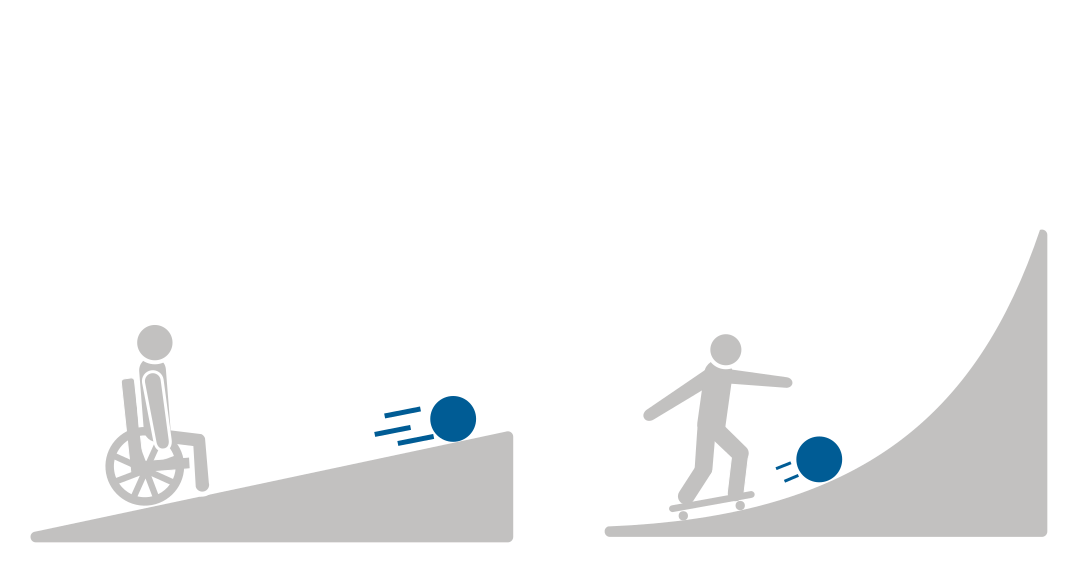
\includegraphics[width=\textwidth]{rampcomparison.png}

Assuming the incline has a constant steepness, the mechanical advantage is equal to the ratio of the length of the inclined plane to the height it rises.

If friction is neglected, the force required to push a weight up the inclined plane is given by:

\[
F_A = \frac{V}{L} F_G
\]

where \( F_A \) is the applied force, \( L \) is the length of the inclined plane, \( V \) is the vertical rise, and \( F_G \) is the gravitational force acting on the mass.

(We haven't yet discussed the sine function, but in case you're familiar with it, note that:

\[
\frac{V}{L} = \sin{\theta}
\]

where \( \theta \) is the angle between the inclined plane and the horizontal surface.)

\begin{Exercise}[title={Ramp}, label=ramp]
A barrel of oil weighs 136 kilograms. You can apply a force of up to 300 newtons. You need to get the barrel onto a platform that is 2 meters high. What is the shortest length of inclined plane you can use?
\end{Exercise}
\begin{Answer}[ref=ramp]
The weight of the barrel is \( 136 \times 9.8 = 1332.8 \) newtons.

Let \( L \) be the length of the inclined plane. The force needed to push the barrel up is related by:

\[
300 = \frac{2}{L} \times 1332.8
\]

Solving for \( L \), we find \( L = \frac{2 \times 1332.8}{300} \approx 8.885 \) meters.
\end{Answer}

\section{Gears}

Gears have teeth that mesh with each other. When you apply torque to one gear, it transfers torque to the other. The resulting torque is increased or decreased depending on the ratio of the number of teeth on the gears.

\includegraphics[width=0.7\textwidth]{gearsNew.png}

If \( N_A \) is the number of teeth on the gear you are turning with a torque of \( T_A \), and \( N_L \) is the number of teeth on the gear it is turning, the resulting torque is:

\[
T_L = \frac{N_A}{N_L} T_A
\]

\begin{Exercise}[title={Gears}, label=gear]
In a bicycle, the goal is not always to gain mechanical advantage, but to spin the pedals slower while applying more force.

You like to pedal your bike at 70 revolutions per minute. The chainring connected to your pedals has 53 teeth. The circumference of your tire is 2.2 meters. You want to ride at 583 meters per minute.

How many teeth should the rear sprocket have?
\end{Exercise}
\begin{Answer}[ref=gear]
The equation relating these quantities is:

\[
583 = 70 \times 2.2 \times \frac{53}{n}
\]

Solving for \( n \), we find \( n = 14 \) teeth.
\end{Answer}

\section{Hydraulics}

In a hydraulic system, such as a car's braking system, you exert force on a piston filled with fluid. The fluid transmits this pressure into another cylinder, where it pushes yet another piston that moves the load.

\includegraphics[width=\textwidth]{hydraulicsNew.png}

The pressure in the fluid is typically measured in pascals (Pa), which is equivalent to \(N / m^2\). We will use pascals for this calculation.

To calculate the pressure you create, divide the force applied by the area of the piston head. To determine the force on the other piston, multiply the pressure by the area of the second piston.

\begin{Exercise}[title={Hydraulics}, label=hydraulics]
Your car has disc brakes. When you apply 2,500,000 pascals of pressure to the brake fluid, the car stops quickly. As the car designer, you want this to require only 12 newtons of force from the driver's foot.

What should the radius of the master cylinder (the piston the driver pushes) be?
\end{Exercise}
\begin{Answer}[ref=hydraulics]
We are solving for the radius \( r \) of the piston. The area of the piston is \( \pi r^2 \), so the pressure is:

\[
\text{Pressure} = \frac{12}{\pi r^2}
\]

Setting the pressure equal to 2,500,000 pascals:

\[
2,500,000 = \frac{12}{\pi r^2}
\]

Solving for \( r \), we find:

\[
r = \sqrt{\frac{12}{\pi \times 2.5 \times 10^6}} \approx 0.00124 \text{ meters}.
\]
\end{Answer}

\graphicspath{{../../Chapters/buoyancy/en_US}}
\chapter{Buoyancy}

The word buoyancy probably brings to mind images of floating in water. Before we dive in, let's zoom out for a moment and consider that the study of buoyancy is about much more than just boats and water. You might be thinking: I want to be a computer programmer, why do I need to know about buoyancy? This topic is much bigger than it might seem at first glance. Buoyancy concerns how all liquids and gasses interact with gravity. The concept of buoyancy is connected to fundamental concepts about how things work in the universe. The \newterm{buoyant force}, as it’s known in engineering, is an important concept that has wide ranging applications. A big part of engineering is moving stuff around, and understanding buoyancy helps us solve problems where we need to move things in and through fluids. Even if you don't have plans to build a robotic submarine, these are super useful ideas to be familiar with. We’ll start exploring the topic with familiar scenarios around boats and water.

When you put a boat into water, it will sink into the water until
the mass of the water it displaces is equal to the mass of the
boat. We think of this in terms of forces. Gravity pulls the mass of
the boat down. The \newterm{buoyant force} pushes the boat up. A boat
dropped into the water will bob up and down a bit before reaching an
\newterm{equilibrium} where the two forces are equal.
% ADD: Explain Action Reaction Pairs in previous chapter
% ADD: Archimedes principle

The buoyant force pushes things up -- against the force of
gravity. The force is equal to the weight of the fluid being
replaced. So, for example, a cubic meter of freshwater has a mass of
about 1000kg.  If you submerge anything with a volume of one meter in
freshwater on earth, the buoyant force will be about 9800 newtons.

For some things, like a block of styrofoam, this buoyant force will be
sufficient to carry it to the surface. Once it reaches the surface, it
will continue to rise (displacing less water) until the mass of the
water it displaces is equal to its mass. And then we say ``It floats!''

\includegraphics[width=.6\textwidth]{waterDisplacement.png}

For some things, like a block of lead, the buoyant force is not
 sufficient to lift it to the surface, and thus we say ``It sinks!''

This is why a helium balloon floats through the air. The air
that it displaces weighs more than the balloon and the helium itself. (It is easy to forget that air has a mass, but it does.)

\begin{Exercise}[title={Buoyancy}, label=buoyancy]
  You have an aluminum box that has a heavy base, so it will always
  float upright. The box and its contents weigh 10 kg. Its base is 0.3 m x 0.4 m. It is 1m tall.

  When you drop it into freshwater ($1000 kg/m^3$), how far will it sink
  before it reaches equilibrium.\index{equilibrium}

\end{Exercise}
\begin{Answer}[ref=buoyancy]
  Equilibrium will be achieved when the box has displaced 10 kg of water. That is, when it has displaced $0.01$ cubic meters.

  The area of the base of the box is 0.12 square meters.  So if the
  box sinks $x$ meters into the water it will displace $0.12 x$ cubic
  meters.

  Thus at equilibrium $x = \frac{0.01}{0.12} \approx 0.083$ m.  So,
  the box will sink 8.3 cm into the water before reaching equilibrium.
\end{Answer}

\section{The Mechanism of Buoyancy: Pressure}

As you dive down in the ocean, you will experience greater and
greater pressure from the water. And if you take a balloon with you, you
will gradually see it get smaller as the water pressure compresses the
air in the balloon.

Let's say you are 3 meters below the surface of the water. What is the
pressure in Pascals (newtons per square meter)? You can think of the
water as a column of water crushing down upon you. The pressure over
a square meter is the weight of 3 cubic meters of water pressing down.

$$p = (3)(1000)(9.8) = 29,400 \text{ Pa }$$

This is called \newterm{hydrostatic pressure}. The general rule for
hydrostatic pressure in Pascals $p$ is

$p = d g h$

Where  $d$ is the density of the fluid
in kg per cubic meter, $g$ is the acceleration due to gravity in
$m/s^2$, and $h$ is the height of the column of fluid above you.

So, where does buoyant force come from? Basically, the pressure pushing up on the
deepest part of the object is higher than the pressure pushing down on
the shallowest part of the object. That is where bouyancy comes from.

\includegraphics[width=.6\textwidth]{buoyancy.png}

\begin{Exercise}[title={Hydrostatic Pressure}, label=mars_pressure]

  You dive into a tank of olive oil on Mars. How much more
  hydrostatic pressure does your body experience at 5 meters deep than
  it did at the surface?

  The density of olive oil is about 900 kg per square meter. The
  acceleration due to gravity on Mars is 3.721 $m/s^2$.

\end{Exercise}
\begin{Answer}[ref=mars_pressure]
$$p = d g h = (900)(3.721)(5) = 16,744.5 \text{ Pa}$$
\end{Answer}

\section{The Mechanism of Buoyancy: Density}
Notice that although the pressure is increasing as you go deeper, the
buoyant force will \emph{not increase} because the buoyant force is always equal
to the weight of the fluid that is displaced, regardless if that is 1
meter or 100 meters underwater.

Due to the added minerals, saltwater is denser than freshwater. This causes objects float
better in the sea than they do in, say, a river. Lipids, like fats and
oils, are less dense than water, allowing them to float on top of a glass of water.
When you're facing a grease fire, you're told not to put water on it. That's because
the water sinks below the grease, then boils, throwing burning grease everywhere.

\graphicspath{{../../Chapters/heat/en_US}}
\chapter{Introduction to the Kontinua Sequence}

This book will start you on the long and difficult trek to becoming a modern
problem solver. Along the path, you will learn how to use the tools of
math, computers, and science.

Why should you bother? There are big problems in this world that will
require expert problem solvers. Those people will make the world a
better place while enjoying interesting and lucrative careers. We are
talking about engineers, scientists, doctors, computer programmers,
architects, actuaries, and mathematicians. Right now, those occupations represent
about 6\% of all the jobs in the United States. Soon,
that number is expected to rise above 10\%.  On average, people in
that 10\% of the population are expected to have salaries twice that
of their non-technical counterparts.\index{career}

Solving problems is difficult. At some point on this journey, you will
see people who are better at solving problems than you are. You, like
every other person who has gone on this journey, will think ``I have
worked so hard on this, but that person is better at it than
I am. I should quit.'' Don't.\index{quitting}

First, solving problems is like a muscle. The more you do, the better
you get at it.  It is OK to say ``I am not good at this yet.'' That
just means you need more practice.

Second, you don't need to be the best in the world. 10 million people
your age can be better at solving problems than you, \textit{and you
  can still be in the top 10\% of the world}. If you complete this
journey, there will be problems for you to solve and a job where your
problem-solving skills will be appreciated.

\emph{Where do we start?}

The famous physicist Richard Feynman once asked this question: ``If,
in some cataclysm, all of scientific knowledge were to be destroyed,
and only one sentence was passed on to the next generation of
creatures, what statement would contain the most information in the
fewest words?''

His answer was ``All things are made of atoms—little particles that move around in
perpetual motion, attracting each other when they are a little
distance apart, but repelling upon being squeezed into one another.''

\emph{That} seems like a good place to start.

\graphicspath{{../../Chapters/biases1/en_US}}
\chapter{Cognitivie Biases 1}


Our brains were designed over millions of years by the evolutionary
process. The resulting mind is an amazing and powerful tool, however
not flawless. The human brain has tendencies (or biases) that nudge us
toward bad judgment and poor decisions.

It would be irresponsible to teach you powerful ideas without
also teaching you about the cognitive biases that follow them. There are about 50
that you should know about, but let's start with only a few.

\section{Fundamental Attribution Error}

You tend to attribute
the mistakes of another person to their character, but attribute your
own mistakes to the situation.

Let's say you are at lunch and someone asks you ``Why was Larry late
for class ?''  You are likely to say ``Larry is lazy
and disorganized.''

If someone asks you ``Why were you late for class last week?''  You
are likely to say, ``I don't remember; The class before it must have
run long.''
\includegraphics[width=0.8\textwidth]{bias_late.png}

The solution? Cut people some slack. You probably don't know the whole
story, so assume that their character is as strong as yours.

Or maybe you also need to hold yourself to a higher standard? Do you find
yourself frequently rationalizing your bad judgment, lateness, or
rudeness?  This could be an opportunity for you to become a better
person whose character is stronger regardless of the situation.

\section{Self-Serving Bias}

\newterm{Self-serving bias} is when you blame the situation for your
failures, but attribute your successes to your strengths.

For example, when asked ``Why did you lose the match?'' you are likely
to answer ``The referee wasn't fair.''  When you are asked ``Why did
you win the match?'' you are likely to answer ``Because I have been
training for weeks, and I was very focused.''
\includegraphics[width=0.8\textwidth]{bias_soccer.png}

This bias tends to make us feel better about ourselves, but it makes it
difficult for us to be objective about our strengths and weaknesses.

\section{In-group favoritism}

\newterm{In-group favoritism}: We tend to favor people who are in
a group with us over people who are not in groups with us.

When asked ``Who is the better goalie, Ted or John?''

If Ted is a Star Trek fan like you, you are likely to think he is also
a good goalie.

As you might imagine, this unconscious tendency is the source of a lot
of subtle discrimination based on race, gender, age, and religion.
\includegraphics[width=0.8\textwidth]{bias_group.png}

\section{The Bandwagon Effect and Groupthink}

\newterm{The bandwagon effect} is our tendency to believe the same
things that the people around us believe. This is how fads spread so
quickly: one person buys in, and then the people they know have a
strong tencdency to buy in as well.

\newterm{Groupthink} is similar: To create harmony with the
people around us, we go along with things we disagree with.

It takes a lot of perspective to recognize when those around us are
wrong. And it takes even more courage to openly disagree with them.

\section{The Curse of Knowledge}

Once you know something, you tend to assume everyone else knows it too.

This is why teaching is sometimes difficult: a teacher will assume
that everyone in the audience already knows the same things the
teacher knows.

Also, when we learn that a friend doesn't know something that we know,
we are often very surprised. This surprise can sometimes manifest as
hurtful behavior.

When I find a gap in a friend's knowledge, I try to remind myself that
the friend certainly knows many things that I don't. I also try to
imagine how it would feel if they teased me for my ignorance.

\section{False Consensus}

We tend to believe that more people agree with us than is actually
the case. For example, if you are a member of a particular religion,
you tend to overestimate the percentage of people in the world who are
members of that religion.

When people vote in elections, they are often surprised when their
preferred candidate loses. ``Everyone, and I mean EVERYONE, voted for
Smith!'' they yell.  ``There must have been a mistake in counting the
votes.''

\section{The Spotlight Effect}

You tend to overestimate how much other people are paying attention to
your behavior and appearance.

Think of six people that you talked to today. Can you even remember what
shoes most of them were wearing? Do you care? Do you think any of them
remember which shoes you wore today?

There is an old saying ``You would worry a lot less about how people
think of you, if you realized how rarely they do.''

\section{The Dunning-Kruger Effect}

The less you know, the more confident you are.

When a person doesn't know all the nuance and context in which a question is
asked, the question seems simple. Thus the person tends to be confident in
their answer. As they learn more about the complexity of the space in
which the question lives, they often realize the answer is not nearly so
obvious.

For example, a lot of people will confidently proclaim ``Taxes are too
high! We need to lower taxes.''  An economist who has studied
government budgets, deficits, history, and monetary policy, might say
something like ``Maybe taxes \emph{are} too high. Or maybe they are
too low. Or maybe we are taxing the wrong things. It is a 
complex question.''

When I am talking with people about a particular topic, I do my best
to defer to the person in the conversation who I think has the most
knowledge in the area. If I disagree with the person, I try to figure
out why our opinions are different.

Similarly, you should assume that any opinion that is voiced, specifically, in an
internet discussion is wildly over-simplified. If you really care
about the subject, read a book by a respected expert. Yes, a whole
book -- there are few interesting topics that can be legitimately
explained in less than 100 pages.

\section{Confirmation Bias}

You tend to find and remember information that supports
beliefs you already have. You tend to avoid and dismiss information
that contradicts your beliefs.

If you believe that intelligent creatures have visited from other
planets, you will tend to look for data to support your beliefs. When
you find data that shows that it is just too far for any creature to
travel, you will try to find a reason why the data is incorrect.

Confirmation bias is one reason why people don't change their beliefs
more often.

Confirmation bias wrecks many, many studies. The person doing the
study often has a hypothesis that they believe and very much want to
prove true. It is very tempting to discard data that doesn't support
the hypothesis. Or maybe the person throws all the data away and experiments again and again until they get the result they want.

When you design an experiment, you must describe it explicitly before
you start. You must tell someone: ``If the hypothesis I love is
incorrect, the results will look like this.  If the hypothesis I love
is correct, the results will look like that. And if the results look
any other way, I have neither proved nor disproved the hypothesis.''

Once the experiment is underway, you must not change the plan and you
must not discard any data.

This is scientific integrity. You should demand it from yourself, and
you should expect it from others.

\section{Survivorship bias}

You will pay more attention to those that survived a process than
those who failed.

After looking at a lot of old houses, you might say ``In the 1880s,
they built great houses.'' However, you haven't seen the houses that
were built in the 1880s and didn't survive. Which houses tended to
survive for a long time? Only the great houses -- you are
basing your opinion on a very skewed sample.


\graphicspath{{../../Chapters/friction/en_US}}
\chapter{Friction}

Imagine there is a large and heavy steel box resting in the middle of a large floor   Imagine you push it hard enough to get it moving.   If you stop pushing,  will it continue to glide gracefully across the floor? 

Probably not.  Unless the floor is very slippery for some reason,  the box will come to a halt immediately after you stop pushing.  We would say that it is stopped by the force of \newterm{friction}. 

What's really happening?  The kinetic energy of the box is being converted into heat 
between the bottom of the box and floor.   As the bottom of the box and the floor get warmer,  the speed of the box decreases.

The amount of friction is proportional to the force with which the box is pressing against the floor -- so you should expect a box that is twice as heavy to experience twice as much frictional force.

That is,  the frictional force is proportional to the normal force.  (FIXME: picture here)

The amount of friction is also determined by the materials that are sliding against each other.  For example,  if the floor is ice,  the frictional force will be less than if the floor is made of wood. 

If you are pushing the box with a force of $F$ and it is moving but neither accelerating nor decelerating,  then the force you are applying is exactly balanced by the frictional force.  If the box is pressing against the floor with a force of $N$, then we say the \newterm{coefficient of friction} between the steel box and the floor is given by

$$\mu = \frac{F}{N}$$

\begin{Exercise}[title={Bicycle Stopping},  label=bike_stop]
  
You are riding your bicycle at 11 meters per second when you slam on the brakes and lock up the wheels.  
You weigh 55 kg.   
When any piece of rubber is skidding across a dry road,  the coefficient of friction will be about 0.7.

Answer the following questions: 

\begin{itemize}
\item How much kinetic energy do you have when you engage the brakes?
\item As you skid,  how much frictional force is decelerating you?
\item For how many meters will you slide?
\end{itemize}

\end{Exercise}
\begin{Answer}[ref=bike_stop]

Kinetic energy? $E = mv^2 = (55)(11^2) = 6,655 \frac{kg m^2}{s^2} = 6,655$ joules.

Frictional force? $F = \mu N = (0.7)(55)(9.8) = 377.3$ newtons.

Distance?  $D = \frac{6,655}{377.3} = 17.6$ seconds.

\end{Answer}

Notice that the force of friction is not determined by how much of the tire is touching the ground.  The coefficient of friction of the two materials and the normal force all all you need to compute the friction.

Why, then, do drag racing cars have such big tires?  Remember that the energy of friction becomes heat and that rubber melts.  If a drag racer had skinny tires,  all the heat from the friction would be in a very small patch of tire, which would melt.

\section{Static vs Dynamic Friction Coefficients}

Once again, imagine the box resting on the floor.  As you start to push it,  it will sit still until your force is greater than the force of friction.   However, once it starts moving,  the force of friction seems to be less.

Between two materials,  there is actually 2 different friction coefficients:

\begin{itemize}
\item Dynamic friction coefficient:  The coefficient you use once the box is sliding against the floor.
\item Static friction coefficient: The coefficient you use to figure out how much force you need to get the box to start to move.
\end{itemize}

The dynamic friction coefficient is always less than the static friction coefficient.  For a car on a dry road,  the dynamic friction coefficient is about 



\graphicspath{{../../Chapters/greek/en_US}}
\chapter{The Greek Alphabet}

If you do anything involving math or physics,  you will use a lot of Greek letters.   Here is a table for your reference:

\begin{tabular}{c c  l | c c l}
Capital & Lower & Pronounced & Capital & Lower & Pronounced\\
\hline
$A$ & $\alpha$ & Alpha & $N$ & $\nu$ & Nu\\
$B$ & $\beta$ & Beta & $\Xi$ & $\xi$ & Xi ("ku-ZY") \\
$\Gamma$ & $\gamma$ & Gamma & $O$ & $o$ & Omicron\\
$\Delta$ & $\delta$ & Delta & $\Pi$ & $\pi$ & Pi\\
$E$ & $\epsilon$ & Epsilon & $P$ & $\rho$ & Rho\\
$Z$ & $\zeta$ & Zeta & $\Sigma$ & $\sigma$ & Sigma\\
$H$ & $\eta$ & Eta & $T$ & $\tau$ & Tau\\
$\Theta$ & $\theta$ & Theta & $\Upsilon$ & $\upsilon$ & Upsilon\\
$I$ & $\iota$ & Iota & $\Phi$ & $\phi$ & Phi\\
$K$ & $\kappa$ & Kappa & $X$ & $\chi$ & Chi ("Kai")\\
$\Lambda$ & $\lambda$ & Lambda & $\Psi$ & $\psi$ & Psi ("Sigh")\\
$M$ & $\mu$ & Mu & $\Omega$ & $\omega$ & Omega
\end{tabular}
\graphicspath{{../../Chapters/basic_statistics/en_US}}
\chapter{Introduction to the Kontinua Sequence}

This book will start you on the long and difficult trek to becoming a modern
problem solver. Along the path, you will learn how to use the tools of
math, computers, and science.

Why should you bother? There are big problems in this world that will
require expert problem solvers. Those people will make the world a
better place while enjoying interesting and lucrative careers. We are
talking about engineers, scientists, doctors, computer programmers,
architects, actuaries, and mathematicians. Right now, those occupations represent
about 6\% of all the jobs in the United States. Soon,
that number is expected to rise above 10\%.  On average, people in
that 10\% of the population are expected to have salaries twice that
of their non-technical counterparts.\index{career}

Solving problems is difficult. At some point on this journey, you will
see people who are better at solving problems than you are. You, like
every other person who has gone on this journey, will think ``I have
worked so hard on this, but that person is better at it than
I am. I should quit.'' Don't.\index{quitting}

First, solving problems is like a muscle. The more you do, the better
you get at it.  It is OK to say ``I am not good at this yet.'' That
just means you need more practice.

Second, you don't need to be the best in the world. 10 million people
your age can be better at solving problems than you, \textit{and you
  can still be in the top 10\% of the world}. If you complete this
journey, there will be problems for you to solve and a job where your
problem-solving skills will be appreciated.

\emph{Where do we start?}

The famous physicist Richard Feynman once asked this question: ``If,
in some cataclysm, all of scientific knowledge were to be destroyed,
and only one sentence was passed on to the next generation of
creatures, what statement would contain the most information in the
fewest words?''

His answer was ``All things are made of atoms—little particles that move around in
perpetual motion, attracting each other when they are a little
distance apart, but repelling upon being squeezed into one another.''

\emph{That} seems like a good place to start.

\graphicspath{{../../Chapters/stat_spreadsheets/en_US}}
\chapter{Introduction to the Kontinua Sequence}

This book will start you on the long and difficult trek to becoming a modern
problem solver. Along the path, you will learn how to use the tools of
math, computers, and science.

Why should you bother? There are big problems in this world that will
require expert problem solvers. Those people will make the world a
better place while enjoying interesting and lucrative careers. We are
talking about engineers, scientists, doctors, computer programmers,
architects, actuaries, and mathematicians. Right now, those occupations represent
about 6\% of all the jobs in the United States. Soon,
that number is expected to rise above 10\%.  On average, people in
that 10\% of the population are expected to have salaries twice that
of their non-technical counterparts.\index{career}

Solving problems is difficult. At some point on this journey, you will
see people who are better at solving problems than you are. You, like
every other person who has gone on this journey, will think ``I have
worked so hard on this, but that person is better at it than
I am. I should quit.'' Don't.\index{quitting}

First, solving problems is like a muscle. The more you do, the better
you get at it.  It is OK to say ``I am not good at this yet.'' That
just means you need more practice.

Second, you don't need to be the best in the world. 10 million people
your age can be better at solving problems than you, \textit{and you
  can still be in the top 10\% of the world}. If you complete this
journey, there will be problems for you to solve and a job where your
problem-solving skills will be appreciated.

\emph{Where do we start?}

The famous physicist Richard Feynman once asked this question: ``If,
in some cataclysm, all of scientific knowledge were to be destroyed,
and only one sentence was passed on to the next generation of
creatures, what statement would contain the most information in the
fewest words?''

His answer was ``All things are made of atoms—little particles that move around in
perpetual motion, attracting each other when they are a little
distance apart, but repelling upon being squeezed into one another.''

\emph{That} seems like a good place to start.

\graphicspath{{../../Chapters/dc1/en_US}}
\chapter{Introduction to Electricity}

What happens when you turn on a flashlight? The battery in the
flashlight acts as an electron pump. The electrons flow through the
wires to the lightbulb (or LED). As the electrons pass through the
lightbulb, they excite the molecules within, which gives off light and
heat. (LEDs also give off light and heat, but they give off a lot less
heat.) Then the electrons return to the battery to be pumped around
again.

When electricity is flowing through a copper wire, the protons and
neutrons of the copper stay put while the electrons jump between the
atoms on their way from the battery to the lightbulb and back again.

In some materials, like copper and iron, electrons are loosely bound
to their nuclei, forming a sea of electrons, which allows energy to flow. These are good \textit{electrical conductors}. In
other materials, like glass and plastic, electrons don't leave their
nuclei easily. Thus, they are terrible electrical conductors -- we call
them \textit{electrical insulators}. For example, the plastic around a
wire is electrical insulation.

\includegraphics[width=0.8\textwidth]{Insulator_vs_Conductor.png}
% KA: https://www.khanacademy.org/science/physics/electric-charge-electric-force-and-voltage/charge-electric-force/v/conductors-and-insulators

\section{Units}

Electrons are very small, so to study them, scientists came up with a
unit that represents \textit{a lot} of electrons. 1 \textit{coulomb}
is about 6,241,509,074,460,762,608 electrons.  When 5 coulombs enter one end of the wire every second (and simultaneously 5 coulombs exit the other end), we say ``This wire is carrying 5 amperes of current.''\index{coulombs}

(Truthfully, we usually shorten ampere to just ``amp''.  This is
sometimes a little awkward because we often shorten the word
``amplifier'' to ``amp''. You should be able to tell which is which
from the context.)\index{amp or ampere}

If you look at the circuit breakers or fuses for your home's
electrical system, you'll see that each one is rated in amps.  For
example, maybe the circuit that supplies power to your kitchen has a 10
amp circuit breaker. If for some reason, more than 10 amps tries to
pass through that wire, the circuit breaker will turn off the whole
circuit.

When it is on, your flashlight pushes about 1 amp of current
through the lightbulb(When it is off, there is no current in the
lightbulb).

\includegraphics[width=0.8\textwidth]{Circuit_OnOff.png}

The lightbulb creates \textit{Resistance} that the current pushes
through.\index{resistance} Think of it like plumbing: The current is the amount of water
passing through a pipe. The resistance is something that tries to stop
the current -- like a ball of hair. The battery is what allows
 the current to push through the resistance; we call that
pressure \textit{voltage}.\index{voltage}

\section{Circuit Diagrams}

Here is a circuit diagram of your flashlight:

\begin{circuitikz}
\draw (0,0) to[battery1,invert,l=$3V$] ++(0,3)
to [switch,i=1A] ++(3,0)
to [lamp=$1\Omega$,bipoles/length=0.9cm] ++(0,-3) -- (0,0);
\end{circuitikz}

The lines are wires.  The symbols that we  will use:

\begin{tabular}{c c c c}
  Battery & Switch & Lamp & Resistor \\
\begin{circuitikz}
\draw (0,0) to[battery1] (2,0); 
\end{circuitikz}
&
\begin{circuitikz}
\draw (0,0) to[lamp,bipoles/length=0.9cm,l=$3 \Omega$] (2,0); 
\end{circuitikz}
&
\begin{circuitikz}
\draw (0,0) to[switch,/tikz/circuitikz/bipoles/length=1.0cm] (2,0); 
\end{circuitikz}
&
\begin{circuitikz}
\draw (0,0) to[R,  l=$3 \Omega$] (2,0); 
\end{circuitikz} \\
\end{tabular}

The battery pushes the electrons from one end and pulls them back in at the other, so the circuit must go around in a circle for the current to flow. This is why the current stops flowing when the switch breaks the circuit.

You can think of a switch as having zero resistance when it is closed and infinite resistance when it is open.


For our purposes, a lamp is just a resistor that gives off light.
% KA: https://www.khanacademy.org/science/high-school-physics/dc-circuits/electric-power-and-dc-circuits/a/circuit-introduction

\section{Ohm's Law}

Resistance is measured in \textit{ohms}, and we use a Greek capital omega for that: $\Omega$  

Voltage is measured in
\textit{volts}.\index{ohms}\index{volts}

\begin{mdframed}[style=important, frametitle={Ohm's Law}]\index{Ohm's law}
  Whenever a voltage $V$ is pushing a current $I$ through a resistance of $I$, the following is true:

  $$V = IR$$

  where $V$ is in volts, $I$ is in amps, and $R$ is in ohms.
\end{mdframed}
% KA: https://www.khanacademy.org/science/physics/circuits-topic/circuits-resistance/v/circuits-part-1

\section{Power and Watts}

\begin{mdframed}[style=important, frametitle={Joule's Law}]\index{Joule's law}

  When a current $I$ is passing through a resistance $R$, the power consumed is
  
  $$W = I^2 R$$

  where $W$ is in watts, $I$ is in amps, and $R$ is in ohms.
\end{mdframed}

Of course $V = IR$, so we can extend this to:

$$W = I^2 R = I V = \frac{V^2}{R}$$

Your flashlight's batteries provide about 3 volts. How much
battery power is the flashlight using when it is on? The power (in
watts) produced by the battery is the product of the voltage (in
volts) and the current (in amps). So your flashlight is giving off $3
volts \times 1 amp = 3 watts$ of power. Some of that power is given
off as light, some as heat.\index{watts}

A watt is 1 joule of energy per second. We say that a watt is a
measure of \textit{power}.

When we talk about how much energy is stored in a battery, we use a
unit like a kilowatt-hour. A kilowatt-hour is equivalent to 3.6 million
joules.

\section{Another great use of RMS}

In many electrical problems, the voltage fluctuates a lot.  For
example, the fluctuations in voltage makes the sound that comes out of an
audio speaker.

You can use the root-mean-squared of the voltage to figure out the average power
your speaker is consuming.

Let's say that the RMS of the voltage you are sending to the speaker is $V_{rms}$
and the resistance of the speaker is $R$ ohms, then the power consumed
by the speaker is:

$$P = \frac{V_{rms}^2}{R}$$

Similarly, if you know the RMS of the current you are pushing through
the speaker is $I_{rms}$, then the power consumed by the speaker is:

$$P = I_{rms} R$$

\section{Electricity Dangers}

Large amounts of electricity moving through your body can hurt or even kill
you. You must be careful around electricity.

However, your body is not a very good conductor, so low-voltage
systems (like a flashlight) don't have enough voltage to move significant amounts of
current through your body.

However, the  electricity in a power outlet has much more voltage. The voltage
in these outlets is fluctuating between positive and negative, so we
call it \textit{Alternating Current} or AC.
% ADD: Introduce difference between AC and dc

\includegraphics[width=0.8\textwidth]{AC_vs_DC.png}

In most countries, the RMS of the voltage between 110 and 240 V. (The
peak voltage is always $\sqrt{2}$ times the RMS value. In the US, for
example, people say ``Our outlets supply 120 V.'' They mean that the
RMS of the voltage difference between the wire and the earth is 120V.
The peak voltage is almost 170V.)

How much current can a human handle? Not much. You can barely feel 1
mA moving through your body, but at 16 mA, your muscles will clench
and you won't be able to relax them -- many people die from
electrocution because they grab a wire which pushes enough current
through their body to prevent them from letting go of the wire.  At 20
mA, a human's respiratory muscles become paralyzed.

The fuse breaker in a house will often allow 20 A to flow through the
circuit before it shuts off the power: Always, always, always shut off
the power before touching any of the wiring in your house.

While water is actually a mediocre conductor, it can still deliver enough current
to kill you. If you see a wire in a puddle, you should not touch the
puddle. Interestingly, because of the salt, sea water is more than
100 times better at conducting electricity than the water you drink.
% ADD: Sea of electrons makes a good conductor

\includegraphics[width=0.8\textwidth]{Sea_Electrons.png}

If you hold a wire in each hand, how many Ohms of resistance will your
body have? Once it gets past your skin, you will look like a bag of
salt water to the electricity. After the skin, your body will have a
resistance of about 300$\Omega$. However, the skin is a pretty good
insulator. If you have dry, calloused hands, your skin may add a
100,000$\Omega$ to the resistance.

% KA: https://www.khanacademy.org/science/in-in-class10th-physics/in-in-electricity/in-in-electric-power-and-heating-effect-of-current/v/electric-power-energy


\graphicspath{{../../Chapters/dc_circuits/en_US}}
\chapter{Introduction to the Kontinua Sequence}

This book will start you on the long and difficult trek to becoming a modern
problem solver. Along the path, you will learn how to use the tools of
math, computers, and science.

Why should you bother? There are big problems in this world that will
require expert problem solvers. Those people will make the world a
better place while enjoying interesting and lucrative careers. We are
talking about engineers, scientists, doctors, computer programmers,
architects, actuaries, and mathematicians. Right now, those occupations represent
about 6\% of all the jobs in the United States. Soon,
that number is expected to rise above 10\%.  On average, people in
that 10\% of the population are expected to have salaries twice that
of their non-technical counterparts.\index{career}

Solving problems is difficult. At some point on this journey, you will
see people who are better at solving problems than you are. You, like
every other person who has gone on this journey, will think ``I have
worked so hard on this, but that person is better at it than
I am. I should quit.'' Don't.\index{quitting}

First, solving problems is like a muscle. The more you do, the better
you get at it.  It is OK to say ``I am not good at this yet.'' That
just means you need more practice.

Second, you don't need to be the best in the world. 10 million people
your age can be better at solving problems than you, \textit{and you
  can still be in the top 10\% of the world}. If you complete this
journey, there will be problems for you to solve and a job where your
problem-solving skills will be appreciated.

\emph{Where do we start?}

The famous physicist Richard Feynman once asked this question: ``If,
in some cataclysm, all of scientific knowledge were to be destroyed,
and only one sentence was passed on to the next generation of
creatures, what statement would contain the most information in the
fewest words?''

His answer was ``All things are made of atoms—little particles that move around in
perpetual motion, attracting each other when they are a little
distance apart, but repelling upon being squeezed into one another.''

\emph{That} seems like a good place to start.

\graphicspath{{../../Chapters/charge/en_US}}
\chapter{Charge}

If you rub a balloon against your hair and then place it next to a wall it will stick. We
say that it has gotten an \textit{electrical charge}. It stole some
electrons from your hair, and now the ballon has slightly more
electrons than protons. We say that it has a negative electrical
charge.

Objects with slightly more protons than electrons have a positive charge.

This charge is measured in coulombs. The charge of a single proton is
about $1.6 \times 10^{-19}$ coulombs.

An object with a negative charge and an object with a positive charge
will be attracted to each other. Two objects with the same charge will
be repelled by each other.
% ADD: Good place for culloms law
% KA: https://www.khanacademy.org/science/hs-physics/x215e29cb31244fa1:types-of-interactions/x215e29cb31244fa1:coulomb-s-law/v/coulombs-law

\begin{mdframed}[style=important, frametitle={Coulomb's Law}]\index{Coulomb's law}

  If two objects with charge $q_1$ and $q_2$ (in coulombs) are $r$ meters from each other, the force of attraction or repulsion is given by

  $$F = K\frac{\lvert q_1 q_2 \rvert}{r^2}$$

    where $F$ is in newtons and $K$ is Coulomb's constant: about $8.988 \times 10^9$.
  
\end{mdframed}


\begin{Exercise}[title={Coulomb's Law}, label=charged_balloons]

Two balloons are charged with an identical quantity and type of
charge: $-5 \times 10^{-9}$ coulombs. They are held apart at a
separation distance of 12 cm. Determine the magnitude of the
electrical force of repulsion between them. 
  
\end{Exercise}
\begin{Answer}[ref=charged_balloons]

  $$F = K\frac{\lvert q_1 q_2 \rvert}{r^2} = (8.988 \times 10^9) \frac{(-5 \times 10^{-9})(-5 \times 10^{-9})}{0.12^2} = \frac{224.7 \times 10^{-9}}{0.0144} = 15.6 \times 10^{-6}$$

  15.6 micronewtons.
  
\end{Answer}

At this point, you might ask ``If the wall has zero
charge, why is the balloon attracted to it?'' The answer: the
electrons in the wall move away from the balloon. The negative charge
on the balloon pushes electrons into the wall, so the surface of the
wall gets a mild positive charge. The surface is close to the balloon,
so the attraction is stronger than the repulsion.

\includegraphics[width=.5\textwidth]{balloon.png}

\section{Lightning}

A cloud is a cluster of water droplets and ice particles. These
droplets and ice particles are always moving up and down through the
cloud. In this process, electrons get stripped off and end up on the
water droplets at the bottom of the cloud( water droplets collect at the bottom because they are denser). The air between the
droplets is a pretty good insulator, and thus the electrons are reluctant
to jump anywhere. However, eventually, the charge gets so strong that
even the insulating properties of the air is not enough to prevent
the jump, causing lightning.
% ADD: Add water density explanation. ice less dense than liquid water due to crystaline structure.

\includegraphics[width=1\textwidth]{lightning.png}

A lot of lightning moves within a cloud or between clouds. However, a
few jump to the earth. These bolts of lightning vary in the amount of
electrons they carry, but the average is about 15 coulombs.

And thunder occurs because the electrons heat the air they pass through, 
causing the air to expand suddenly, and the resulting shockwave is the sound we know as thunder.
% ADD: Relate speed of light and sound 
\section{But...}

This idea that opposite charges attract creates some heavy questions
that you do not yet have the tools to work with. So the answer is
basically ``Don't ask that question now!''

However, you probably have these questions, so I will point you in
the direction of the answers.

The first is ``In any atom bigger than hydrogen, there are multiple
protons in the nucleus. Why don't the protons push each other out of
the nucleus?''

We aren't ready to talk about it, but there is a force called \textit{the
 nuclear force} which pulls the protons and neutrons in the nucleus
of the atom toward each other. At very, very small distances it is
strong enough to overpower the repulsive force due to the protons'
charges.
% ADD: Effective nuclear charge

Another question is ``Why do the electrons whiz around in a cloud so
far from the nucleus of the atom? Negatively charged electrons should
cling to the protons in the center, right?''

We aren't ready to talk about it, but quantum mechanics tells us that
electrons like to live in a certain specific energy level. Hugging
protons isn't one of those levels.

\graphicspath{{../../Chapters/fertilizer/en_US}}
\chapter{Fertilizer}

FIXME 
First, Allison has learned she does not need a colon after FM

\textit{Here are some thoughts on expanding the introduction to the Fertilizer Chapter. This might be a good moment to discuss the multidisciplinary nature of Kontinua. 
In a regular science class I'm guessing you wouldn't get electricity and Fertilizer in the same textbook. Why is there a chapter on Fertilizer here? Are you introducing us to the major ways science has given us more power and allowed population to grow? Can we discuss your thoughts on why problem solvers need a basic understanding of Fertilizer and I'll write up a new introduction to this chapter based on the discussion?}

\textit{What do you think about adding a conclusion that talks about the connection between fertilizer (nitrogen), dynamite and the origin of the Nobel peace prize? I know you don't want too much history and philosophy but this seems like a great moment to add a little narrative spice}.

Chapter text starts here: 


In 1950, there were 2.5 billion people on the planet, and about 65\%
were malnourished. In 2019, there were 7.7 billion people on the
planet, and only 15\% are malnourished. How did crop yields increase
so much? There were several factors: better crop varieties,
reliable irrigation, increased mechanization, and affordable fertilizers.\index{fertilizer}

When a plant grows, it takes molecules out of the soil and uses them
to build proteins. It primarily needs the elements nitrogen ($N$),
phosphorus ($P$), and potassium ($K$).\index{nitrogen} \index{phosphorus} \index{potassium}

When you buy a bag of fertilizer at the store, it typically has
three numbers on the front.  For example, you might buy a bag of
``24-22-4''.  This means that 24\% of the mass of the bag is nitrogen,
22\% is phosphorus, and 4\% is potassium.

Potassium comes as potassium carbonate ($K_2CO_3$), potassium chloride
($KCl$), potassium sulfate ($K_2 SO_4$), and potassium nitrate
($KNO_3$). Any blend of these chemicals is known as ``potash''. Potash
is dug up out of mines. \index{potash}

Phosphorus is also mined, but is refined into phosphoric acid
($H_3PO_4$) before it is put into fertilizer.

Nitrogen is an especially interesting case for 2 reasons:
\begin{itemize}
\item Worldwide farmers apply more nitrogen to their soil than potassium or phosphorous combined.
\item 78\% of the air we breathe is nitrogen in the form of $N_2$, but
  neither plants nor animals can utilize nitrogen in that form.
\end{itemize}

\section{The Nitrogen Cycle}

Converting the $N_2$ in the air into a form that a plant can use
is known as \newterm{nitrogen fixation}. For billions of years, there
were only two ways that nitrogen fixation occurred on earth:
\begin{itemize}
\item The energy from lightning causes $N_2$ and $H_2O$ to reconfigure as ammonia ($NH_3$) and nitrate ($NO_3$). This accounts for about 10\% of all naturally occurring nitrogen fixation.
\item Cyanobacteria are responsible for the rest. They convert $N_2$ into ammonia.
\end{itemize}\index{nitrogen cycle} \index{nitrogen fixation}

Let's say that you are eating soybeans. There is a cyanobacteria
called \newterm{rhizobia} that has a symbiotic relationship with
soybean plants.  Rhizobia fixes nitrogen for the soybean plant. The
soybean plant performs photosynthesis and gives sugars to the
rhizobia.

The proteins in the soybeans contain nitrogen from the rhizobia. When
you eat them, you use some of the nitrogen to build new proteins. You
probably don't use all the nitrogen, so your cells release ammonia into your blood.

Ammonia likes to react with things, so your liver combines the ammonia
with carbon dioxide to make urea ($CO(NH_2)_2$).  Your kidneys take
the urea out of your blood and mix it with a bunch of water and salts
in your bladder.  When you urinate, the urea leaves your body.\index{urea}

If you urinate on the ground, the nearby plants can take the nitrogen out of
the urea.\index{urine}

When you die, the nitrogen in your proteins will return to the soil as
ammonia and nitrate.

For centuries, farms got their nitrogen from urine, feces, and rotting
organic material. There were two challenges with this:
\begin{itemize}
\item Human pathogens had to be kept away from human food.
\item There was simply not enough to support 7.7 billion people.
\end{itemize}

So we had to figure out how to do nitrogen fixation at an industrial
level.

\section{The Haber-Bosch Process}

During World War I, two German scientists, Fritz Haber and Carl Bosch
figured out how to make ammonia from $N_2$ and $H_2$ using high
temperatures and pressures. This is how nearly all nitrogen fertilizer
is created today.\index{Haber-Bosch process}

Where do we get the $H_2$? From methane ($CH_4$) in natural gas. Today, 3-5\%
of the world's natural gas production is consumed in the Haber-Bosch
process.

The ammonia is converted into ammonium nitrate ($NH_4NO_3$) or urea
before it is shipped to farms.

\section{Other nutrients}

Healthy plants require several other elements that are sometimes
applied as fertilizer: calcium, magnesium, and sulfur.

Finally, tiny amounts of copper, iron, manganese, molybdenum, zinc, and
boron are sometimes needed.

\graphicspath{{../../Chapters/concrete/en_US}}
\chapter{Concrete}

To make concrete, you mix cement with water and an aggregate (sand or
rock).  The cement is usually only about 10 to 15 percent of the
mixture. The cement reacts with the water, and the resulting solid
binds the aggregate together. In 2019, the world consumed 4.5 billion
tons of cement.\index{concrete} \index{cement}

Concrete is hard and durable. The mortar between the pyramids at Giza
is concrete -- it is now 5000 years old. Today we use concrete to
build many structures including buildings, bridges, airport runways,
and dams.

There are many kinds of cement, but the most common is Portland
cement. It is made by heating limestone (calcium carbonate) with clay
(for silicon) in a kiln. Two things come out of the kiln: Carbon
dioxide and a hard substance called ``clinker''.  The clinker is
ground up with some gypsum before it is sent to market.

The carbon dioxide is released into the atmosphere. Cement manufacture
is responsible for about 8\% of the world's $CO_2$ emissions; it is a
major contributor to climate change.

Really hard concrete, like that used in a nuclear power plant, can
support 3,000 kg per centimeter without being crushed.  However, if
you pull on two ends of a piece of concrete it comes apart pretty
easily. We say that concrete can handle a lot of \newterm{compressive
  stress}, but not much \newterm{tensile} stress.

\section{Steel reinforced concrete}

Many places where we use concrete (like in a bridge), we need both
compressive and tensile stress.  Often the top of a beam is undergoing
compression and the bottom of the beam is undergoing tension.

FIXME Picture here

Steel has tremendous tensile strength, but not as much compressive
strength as concrete. To get both tensile \emph{and} compressive
strength, we often bury steel bars or cables inside the concrete.
This is known as \newterm{steel-reinforced concrete}. The concrete
generally does a very good job protecting the steel, which keeps it
from rusting.\index{steel reinforced concrete}

You may have heard of \newterm{rebar}.  That is just short for
``reinforcing bar''.  Typically rebar has bumps and ridges that keep
the bar and the concrete from moving independently.\index{rebar}

\section{Recycling concrete}

A lot of concrete structures only last about 100 years. When they are
demolished, the concrete can be reused as aggregate in other projects.
Often the concrete bits are mixed with cement and made into concrete again.

If the concrete to be reused is reinforced with steel, the steel has
to be removed and recycled separately.  Then the concrete is crushed
into small pieces.

\graphicspath{{../../Chapters/metals/en_US}}
\chapter{Metals}

Elements that transmit electricity well, even at low temperatures, are
called \newterm{metals}. Here are some metals that you are probably familiar
with: aluminum, iron, copper, tin, gold, silver, and platinum. Aluminum and
iron are particularly common; together they make up about 14\% of the
earth's crust.

An \newterm{alloy} is a mixture of elements that includes at least one
metal. Brass, for example, is an alloy of copper and zinc.  Bronze is
an alloy of copper and tin.

\section{Steel}

One of the most common alloys is steel, an alloy of iron and carbon.
In pure iron, the molecules slip easily past each other, so pure iron
is relatively soft and easily deformed. The carbon in steel prevents
that slipping, thus steel is much, much harder than iron.

How much carbon? If you put less than 0.002\% by weight, you end up
with something very much like pure iron.  As you increase the carbon,
it gets harder and harder.  Once it gets above about 2\%, the result
is very brittle.

If you add about 11\% chromium to steel, you get \newterm{stainless
  steel} which resists rusting.

\begin{Exercise}[title={Tensile Strength}, label=tensile-mpa]

The tensile strength of steel is usually between 400 MPa and 1200
MPa. A Mega Pascal (MPa) is the strength necessary to hold 1,000,000 newtons of
force with a cable that has a 1 square meter cross section. Or,
equivalently, to hold 1 newton of force with a cable that has a 1
square millimeter cross section. 

If you have are buying a round cable that has a tensile strength of
700 Mpa and must hold a 100 kg man aloft, what the diameter of the
smallest cable you can use?
  
\end{Exercise}
\begin{Answer}[ref=tensile-mpa]
On earth, holding a 100 kg man aloft requires 980 Newtons of force.

$980/700 = 1.4$, so you need a cable with a cross-section area of 1.4
square millimeters.

$$\pi r^2 = 1.4$$

So $r = \sqrt{1.4/\pi} \approx .67$ millimeters.  So the cable would
have to have a diameter of at least 1.34 millimeters.

\end{Answer}

Here are some approximate tensile strengths of ather materials:

\begin{tabular}{c|c}
  Material & Tensile strength (MPa) \\
  \hline
  Iron & 3 \\
  Concrete & 4 \\
  Rubber & 16 \\
  Glass & 33 \\
  Wood & 40 \\
  Nylon & 100 \\
  Human hair & 200 \\
  Aluminum  & 300 \\
  Steel & 700 \\
  Spider webs & 1000 \\
  Carbon fiber & 4000
\end{tabular}

\section{What metal for what task?}

You will see copper used a lot for electrical wires in your house and
appliances because it is very efficient at moving electricity (very
little power is lost as heat). It is also very good a transmitting
heat, so you will often see copper pots and pans.

Aluminum is less dense than copper, and is still a pretty good
conductor of electricity. Thus, the overhead wires in a power system
are often made of aluminum.

Aluminum is not as strong as steel, but considerably lighter. It is
often used structurally where weight is a concern: skyscrapers, cars,
airplanes, and ships.

Titanium is about as strong as steel, but it weights about half as
much. Titanium is very difficult to work with, so it is used in places
where weight and strength are very important and cost is not:
airplanes and bicycles.

(Carbon fiber, which is light, strong, and very easy to work with, is
replacing aluminum and titanium in many applications. 20 years ago,
many expensive bicycles were made of titanium. These days the vast
majority are made with carbon fiber.)

Zinc and tin are very resistant to corrosion, so they are often used
as a coating to prevent steel from rusting. They are also used in many
alloys for the same reason.  In the United States, the penny is 97.5\%
zinc and only 2.5\% copper.


\graphicspath{{../../Chapters/angles/en_US}}
\chapter{Introduction to the Kontinua Sequence}

This book will start you on the long and difficult trek to becoming a modern
problem solver. Along the path, you will learn how to use the tools of
math, computers, and science.

Why should you bother? There are big problems in this world that will
require expert problem solvers. Those people will make the world a
better place while enjoying interesting and lucrative careers. We are
talking about engineers, scientists, doctors, computer programmers,
architects, actuaries, and mathematicians. Right now, those occupations represent
about 6\% of all the jobs in the United States. Soon,
that number is expected to rise above 10\%.  On average, people in
that 10\% of the population are expected to have salaries twice that
of their non-technical counterparts.\index{career}

Solving problems is difficult. At some point on this journey, you will
see people who are better at solving problems than you are. You, like
every other person who has gone on this journey, will think ``I have
worked so hard on this, but that person is better at it than
I am. I should quit.'' Don't.\index{quitting}

First, solving problems is like a muscle. The more you do, the better
you get at it.  It is OK to say ``I am not good at this yet.'' That
just means you need more practice.

Second, you don't need to be the best in the world. 10 million people
your age can be better at solving problems than you, \textit{and you
  can still be in the top 10\% of the world}. If you complete this
journey, there will be problems for you to solve and a job where your
problem-solving skills will be appreciated.

\emph{Where do we start?}

The famous physicist Richard Feynman once asked this question: ``If,
in some cataclysm, all of scientific knowledge were to be destroyed,
and only one sentence was passed on to the next generation of
creatures, what statement would contain the most information in the
fewest words?''

His answer was ``All things are made of atoms—little particles that move around in
perpetual motion, attracting each other when they are a little
distance apart, but repelling upon being squeezed into one another.''

\emph{That} seems like a good place to start.

\graphicspath{{../../Chapters/triangles_circles/en_US}}
\chapter{Introduction to the Kontinua Sequence}

This book will start you on the long and difficult trek to becoming a modern
problem solver. Along the path, you will learn how to use the tools of
math, computers, and science.

Why should you bother? There are big problems in this world that will
require expert problem solvers. Those people will make the world a
better place while enjoying interesting and lucrative careers. We are
talking about engineers, scientists, doctors, computer programmers,
architects, actuaries, and mathematicians. Right now, those occupations represent
about 6\% of all the jobs in the United States. Soon,
that number is expected to rise above 10\%.  On average, people in
that 10\% of the population are expected to have salaries twice that
of their non-technical counterparts.\index{career}

Solving problems is difficult. At some point on this journey, you will
see people who are better at solving problems than you are. You, like
every other person who has gone on this journey, will think ``I have
worked so hard on this, but that person is better at it than
I am. I should quit.'' Don't.\index{quitting}

First, solving problems is like a muscle. The more you do, the better
you get at it.  It is OK to say ``I am not good at this yet.'' That
just means you need more practice.

Second, you don't need to be the best in the world. 10 million people
your age can be better at solving problems than you, \textit{and you
  can still be in the top 10\% of the world}. If you complete this
journey, there will be problems for you to solve and a job where your
problem-solving skills will be appreciated.

\emph{Where do we start?}

The famous physicist Richard Feynman once asked this question: ``If,
in some cataclysm, all of scientific knowledge were to be destroyed,
and only one sentence was passed on to the next generation of
creatures, what statement would contain the most information in the
fewest words?''

His answer was ``All things are made of atoms—little particles that move around in
perpetual motion, attracting each other when they are a little
distance apart, but repelling upon being squeezed into one another.''

\emph{That} seems like a good place to start.

\graphicspath{{../../Chapters/pythagorean_theorem/en_US}}
\chapter{Introduction to the Kontinua Sequence}

This book will start you on the long and difficult trek to becoming a modern
problem solver. Along the path, you will learn how to use the tools of
math, computers, and science.

Why should you bother? There are big problems in this world that will
require expert problem solvers. Those people will make the world a
better place while enjoying interesting and lucrative careers. We are
talking about engineers, scientists, doctors, computer programmers,
architects, actuaries, and mathematicians. Right now, those occupations represent
about 6\% of all the jobs in the United States. Soon,
that number is expected to rise above 10\%.  On average, people in
that 10\% of the population are expected to have salaries twice that
of their non-technical counterparts.\index{career}

Solving problems is difficult. At some point on this journey, you will
see people who are better at solving problems than you are. You, like
every other person who has gone on this journey, will think ``I have
worked so hard on this, but that person is better at it than
I am. I should quit.'' Don't.\index{quitting}

First, solving problems is like a muscle. The more you do, the better
you get at it.  It is OK to say ``I am not good at this yet.'' That
just means you need more practice.

Second, you don't need to be the best in the world. 10 million people
your age can be better at solving problems than you, \textit{and you
  can still be in the top 10\% of the world}. If you complete this
journey, there will be problems for you to solve and a job where your
problem-solving skills will be appreciated.

\emph{Where do we start?}

The famous physicist Richard Feynman once asked this question: ``If,
in some cataclysm, all of scientific knowledge were to be destroyed,
and only one sentence was passed on to the next generation of
creatures, what statement would contain the most information in the
fewest words?''

His answer was ``All things are made of atoms—little particles that move around in
perpetual motion, attracting each other when they are a little
distance apart, but repelling upon being squeezed into one another.''

\emph{That} seems like a good place to start.

\graphicspath{{../../Chapters/congruence/en_US}}
\chapter{Introduction to the Kontinua Sequence}

This book will start you on the long and difficult trek to becoming a modern
problem solver. Along the path, you will learn how to use the tools of
math, computers, and science.

Why should you bother? There are big problems in this world that will
require expert problem solvers. Those people will make the world a
better place while enjoying interesting and lucrative careers. We are
talking about engineers, scientists, doctors, computer programmers,
architects, actuaries, and mathematicians. Right now, those occupations represent
about 6\% of all the jobs in the United States. Soon,
that number is expected to rise above 10\%.  On average, people in
that 10\% of the population are expected to have salaries twice that
of their non-technical counterparts.\index{career}

Solving problems is difficult. At some point on this journey, you will
see people who are better at solving problems than you are. You, like
every other person who has gone on this journey, will think ``I have
worked so hard on this, but that person is better at it than
I am. I should quit.'' Don't.\index{quitting}

First, solving problems is like a muscle. The more you do, the better
you get at it.  It is OK to say ``I am not good at this yet.'' That
just means you need more practice.

Second, you don't need to be the best in the world. 10 million people
your age can be better at solving problems than you, \textit{and you
  can still be in the top 10\% of the world}. If you complete this
journey, there will be problems for you to solve and a job where your
problem-solving skills will be appreciated.

\emph{Where do we start?}

The famous physicist Richard Feynman once asked this question: ``If,
in some cataclysm, all of scientific knowledge were to be destroyed,
and only one sentence was passed on to the next generation of
creatures, what statement would contain the most information in the
fewest words?''

His answer was ``All things are made of atoms—little particles that move around in
perpetual motion, attracting each other when they are a little
distance apart, but repelling upon being squeezed into one another.''

\emph{That} seems like a good place to start.

\graphicspath{{../../Chapters/parallel_perpendicular/en_US}}
\chapter{Parallel and Perpendicular}

Two vectors are said to be parallel if they have the same or opposite direction. In simpler terms, if two vectors are pointing in the same direction (even if their magnitudes differ), they are considered parallel. For example, imagine you have a vector representing the direction and speed of a car moving north. If you have another vector representing the direction and speed of a different car also moving north, these vectors are parallel.

On the other hand, if two vectors point in completely opposite directions, they are still considered parallel. For instance, if one vector represents a car moving north and the other represents a car moving south, these vectors are parallel but in opposite directions.

Perpendicular vectors, as the name suggests, are vectors that intersect each other at a right angle, forming a 90-degree angle. If we imagine a sheet of paper, drawing a horizontal vector and a vertical vector on that paper would create perpendicular vectors. In this case, the horizontal vector represents left-right direction, while the vertical vector represents up-down direction. Perpendicular vectors are often seen in geometric shapes, such as squares and rectangles, where their sides intersect at right angles.

A fundamental property of perpendicular vectors is that their dot product is zero. The dot product is a mathematical operation that measures the extent to which two vectors align with each other. When two vectors are perpendicular, their dot product is always zero. This property provides a useful tool for determining whether two given vectors are perpendicular.

Understanding parallel and perpendicular vectors is essential in various areas of mathematics and physics. For example, in geometry, knowledge of perpendicular vectors helps us determine whether lines are perpendicular or parallel. In physics, vectors can represent forces, velocities, or displacements, and identifying parallel or perpendicular vectors aids in analyzing motion and forces acting on objects.

In summary, parallel vectors have the same or opposite direction, while perpendicular vectors intersect at a right angle. Recognizing these relationships between vectors enables us to solve problems involving geometry, physics, and many other fields. As you delve deeper into the exciting world of vectors, keep an eye out for parallel and perpendicular relationships, as they often hold valuable insights and solutions.

\graphicspath{{../../Chapters/circles/en_US}}
\chapter{Circles}

A circle is the set of points $(x, y)$ that are a particular distance $r$ from a
particular point $(x_c, y_c)$.  We say that $r$ is the
\newterm{radius} and $(x_c, y_c)$ is the \newterm{center}

\begin{tikzpicture}
    \filldraw [sdkblue] (1,2) circle (2pt) node[anchor=west]{$(x_c, y_c)$};
    \filldraw [sdkblue] (2,4.82842712474619) circle (2pt) node[anchor=west]{$(x, y)$};
    \draw [sdkblue,dashed](1,2) -- (2,4.82842712474619) node[midway,anchor=west] {$r$};
    \draw [sdkblue](1,2) circle (3);
    \draw [stealth-stealth](-2.5,0)--(4.5,0);
    \draw [stealth-stealth](0,-1.5)--(0,5.5);
\end{tikzpicture}

\begin{mdframed}[style=important, frametitle={Area and Radius}]

  If the radius of a circle is $r$, the area of its interior ($a$) is given by \index{circle!area of}

  $$a = \pi r^2$$

\end{mdframed}

\begin{Exercise}[title={Area of a Circle}, label=area_of_circle]

  The paint you have says ``One liter covers 6 square meters.''

  You are painting the top of a circular table with a radius of 3 meters.

  How much paint will you need?
  
\end{Exercise}
\begin{Answer}[ref=area_of_circle]

  The table has a radius of 3 meters.

  So the area of its top is $3^2 \pi \approx 28.27$.

  $$ 28.27 \text{ square meters }\left(\frac{1 \text{ liter }}{6 \text{ square meters }} \right) = 4.72 \text{ liters }$$ 
  
\end{Answer}


Note that a circle lives in a particular plane. The points $(x, y, z)$ that are a particular distance $r$ from a
particular point $(x_c, y_c, z_c)$ are a sphere:

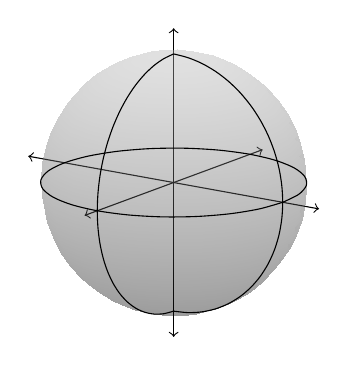
\begin{tikzpicture}
  \begin{axis}[
    view={35}{15},
    unit vector ratio=1 1 1,
    ticks = none,
    axis lines=middle,
    ymin=-3.5,
    ymax=3.5,
    xmax=4.0,
    xmin=-4.0,
    zmin=-3.6,
    zmax=3.6,
    x axis line style=<->,
    y axis line style=<->,
    z axis line style=<->,
    clip=false
    ]
    \addplot3[surf,shader=interp,domain=0:360,y domain=-90:90, opacity=0.4,
    colormap={blackwhite}{color=(black) color=(black!30)}] ({3 * cos(y) * cos(x)},
    {3 *  cos(y) * sin(x)},{3 * sin(y)});
    \addplot3[samples y=0,domain=0:360,smooth]({3*cos(x)}, {3*sin(x)}, 0.0);
    \addplot3[samples y=0,domain=-180:0,smooth](0, {3*sin(x)}, {3*cos(x)});
    \addplot3[samples y=0,domain=0:180,smooth]({3*sin(x)}, 0, {3*cos(x)});
  \end{axis}
\end{tikzpicture}

The distance all the way across the middle of a circle (or a sphere) is its
\newterm{diameter}.  The diameter is always twice the radius.

For the rest of the chapter, we are talking about circles, points, and
lines \textit{in a plane}.

\begin{mdframed}[style=important, frametitle={Circumference and Diameter}]

  The circumference ($c$) of a circle is the distance around the circle. If the diameter is $d$, \index{circumference}

  $$c = \pi d$$

\end{mdframed}

\begin{Exercise}[title={Circumference}, label=circumference]

  Using a tape measure, you figure out that the circumference of a tree in your yard is 64 cm.

  Assuming the trunk is basically circular,  what is its diameter?
  
\end{Exercise}
\begin{Answer}[ref=circumference]

  The diameter is $$\frac{c}{\pi} = \frac{64}{\pi} \approx 20.37 \text{ centimeters}$$
  
\end{Answer}
\begin{Exercise}[title={Splitting a Pie}, label=pie_splitting]

  A pie has a radius of 13 cm.  7 friends all want equal sized wedges.  You have a tape measure.

  How many centimeters will each outer crust be?

\end{Exercise}
\begin{Answer}[ref=pie_splitting]

  The circumference of the pie is $26 \pi \approx 81.7$ centimenters.
  
  The length of the crust for each piece would be about $\frac{81.7}{7} = 11.7$ cm.

  
\begin{tikzpicture}
    \filldraw [black] (0,0) circle (2pt);
    \draw [black](0,0) circle (3);
    \foreach \x in {0,...,6}
    \draw [dashed] (0,0) -- ({3 * cos(\x * 51.428571428571429)}, {3 * sin(\x * 51.428571428571429)});
    \draw [sdkblue,very thick] (3, 0) arc (0:51.43:3) node [midway, anchor=east] {11.7 cm};
    \node at (1.0, 1.5)  {13 cm};
\end{tikzpicture}
\end{Answer}



\begin{mdframed}[style=important, frametitle={Length of an Arc}]

If you have two points $a$ and $b$ on a circle, the ray from the
center through $a$ and the ray from the center through $b$ form an
angle.  If $\theta$ is the angle in radians and $r$ is the radius of
the circle, the distance from $a$ to $b$ on the circle is $r \theta$.

\begin{tikzpicture}
    \filldraw [black] (0,0) circle (2pt) node[anchor=west]{Center};
    \filldraw [sdkblue] (-1,2.82842712474619) circle (2pt) node[anchor=west]{$b$};
    \filldraw [sdkblue] (2.12132,2.12132) circle (2pt) node[anchor=east]{$a$};
    \draw [sdkblue,dashed,->](0,0) -- (-1.2,3.394112549695428);
    \draw [sdkblue,dashed,->](0,0) -- (2.4, 2.4) node[midway,anchor=east]{$r$};
    \draw [black](0,0) circle (3);
    \draw [sdkblue,very thick] (2.12132,2.12132) arc (45:109.47:3) node [midway, anchor=south] {$r \theta$};
    \draw [sdkblue, <->] (0.707,0.707) arc (45:109.47:1) node [midway, anchor=south]{$\theta$};
\end{tikzpicture}

\end{mdframed}

\begin{Exercise}[title={Arc Length}, label=arc_length]

You have been asked to find the radius of a very large cylindrical tank.
You have a tape measure, but it is only 15 meters long and doesn't
reach all the way around the tank.

However, you have a compass.  So you stick one end of the tape measure
to the side of the tank and measure the orientation of the wall at
that point.  Then you walk the 15 meters and measure the orientation of the wall there.

You find that 15 meters represents 72 degrees of arc.

What is the radius of the tank in meters?
  
\end{Exercise}
\begin{Answer}[ref=arc_length]

  $$72 \text{ degrees } \left(\frac{2\pi \text{ radians }}{360 \text{ degrees }}\right) \approx 1.2566 \text{ radians }$$

  $$15 = 1.2566r$$

  $$r = 11.94 \text{ meters}$$
  
\begin{tikzpicture}
    \filldraw [black] (0,0) circle (2pt);
    \draw [black](0,0) circle (3);
    \draw [dashed] (0,0) -- ({3 * cos(72)}, {3 * sin(72)});
    \draw [dashed] (0,0) -- (3, 0);
    \draw [sdkblue,very thick] (3,0) arc (0:72:3) node [midway, anchor=east] {15 m};
    \draw [sdkblue, <->] (1,0) arc (0:72:1) node [midway, anchor=east]{$72^\circ$ = 1.2566 rad};
    \node at (0.0, 1.6)  {11.94 m};
\end{tikzpicture}
\end{Answer}

\section{Tangents}

A line that is \newterm{tangent} to a circle touches it at exactly one point:

\begin{tikzpicture}
    \filldraw [black] (0,0) circle (2pt);
    \draw [dashed, black](0,0) circle (3);
    \filldraw [sdkblue] (2.121, 2.121) circle (2pt);
    \draw [sdkblue, thick] (6.243, -2) -- (0, 4.243);
\end{tikzpicture}

The tangent line is always perpendicular to the radius to the point of tangency:

\begin{tikzpicture}
  \filldraw [black] (0,0) circle (2pt);
  \draw [dashed, black](0,0) circle (3);
  \filldraw [sdkblue] (2.121, 2.121) circle (2pt);
  \draw [sdkblue, thick] (0,0) -- (2.121, 2.121);
  \draw [black] (1.9, 1.9) -- (2.121, 1.679) -- (2.342,1.9);
  \draw [sdkblue, thick] (6.243, -2) -- (0, 4.243);
\end{tikzpicture}


\begin{Exercise}[title={Painting a Comet}, label=painting_comet]
  
  You have been asked to paint a comet and its tail in yellow on the floor of a gymnasium.

  A liter of yellow paint covers 6 square meters.

  First you draw a circle with a radius of 3 meters.  Then you mark a
  point $D$ on the floor 7 meters from the center of the circle.  Then
  you draw two tangent lines that pass through $D$.

  You use a protractor to measure the angle at which the tangent lines meet: about $51^\circ$
  
  \begin{tikzpicture}
    \filldraw [sdkblue] (0,0) circle (2pt);
    \filldraw [black] (7,0) circle (2pt);
    \draw [sdkblue,dashed] (0,0) -- (3,0) node [midway, anchor=south] {3 m};
    \draw [sdkblue,dashed] (3,0) -- (7,0) node [midway, anchor=south] {4 m};
    \draw [sdkblue,dashed, ->] (5.5,0) arc (180:154.6:1.5) node [midway, anchor=west]{$51^\circ$};
    \draw [sdkblue,dashed, ->] (5.5,0) arc (180:205.4:1.5);
    \draw [black,thick] (7,0) -- ({3 * cos(64.62)}, {3 * sin(64.62)});
    \draw [black,thick] (7,0) -- ({3 * cos(-64.62)}, {3 * sin(-64.62)});
    \filldraw [black] ({3 * cos(64.62)}, {3 * sin(64.62)}) circle (2pt);
    \filldraw [black] ({3 * cos(-64.62)}, {3 * sin(-64.62)}) circle (2pt);
    \filldraw [sdkblue] (3, 0) circle (2pt);
    \draw [sdkblue,dashed] ({3 * cos(-64.62)}, {3 * sin(-64.62)}) arc (-64.62:64.62:3);
    \draw [black,thick] ({3 * cos(64.62)}, {3 * sin(64.62)}) arc (64.62:295.38:3);
  \end{tikzpicture}

  Before you paint the area contained by the circle and the two
  tangent lines, how much paint will you need?
    

\end{Exercise}
\begin{Answer}[ref=painting_comet]

  The trick here is to take advantage of the fact that the tangent is perpendicular to the radius to make right triangles:

  \begin{tikzpicture}
    \coordinate (a) at ({3 * cos(64.62)}, {3 * sin(64.62)});
    \coordinate (b) at ({3 * cos(-64.62)}, {3 * sin(-64.62)});
    \filldraw [sdkblue] (0,0) circle (2pt);
    \filldraw [black] (7,0) circle (2pt);
    \draw [black,thick] (0,0) -- (a) node [midway, anchor=east] {3m};
    \draw [black,thick] (0,0) -- (b) node [midway, anchor=east] {3m};
    \draw [black,thick] (0,0) -- (7,0) node [midway, anchor=south] {7 m};
    \draw [sdkblue,dashed, <->] (5.5,0) arc (180:154.6:1.5) node [midway, anchor=west]{$25.5^\circ$};
    \draw [sdkblue,dashed, <->] (5.5,0) arc (180:205.4:1.5) node [midway, anchor=west]{$25.5^\circ$};
    \draw [sdkblue,dashed, <->] (1.5,0) arc (0:64.5:1.5) node [midway, anchor=west]{$64.5^\circ$};
    \draw [sdkblue,dashed, <->] (1.5,0) arc (0:-64.5:1.5) node [midway, anchor=west]{$64.5^\circ$};
    \draw [black,thick] (7,0) -- (a);
    \draw [black,thick] (7,0) -- (b);
    \filldraw [black] (a) circle (2pt);
    \filldraw [black] (b) circle (2pt);
    \draw [black,thick] (a) arc (64.62:295.38:3);
  \end{tikzpicture}

  The wedge has radius 3 and represents $360 - 2(64.5) = 231^\circ \approx 4.03 \text{ radians}$.

  We are finding the area of this piece:
  
  \begin{tikzpicture}
    \coordinate (a) at ({3 * cos(64.62)}, {3 * sin(64.62)});
    \coordinate (b) at ({3 * cos(-64.62)}, {3 * sin(-64.62)});
    \filldraw [sdkblue] (0,0) circle (2pt);
    \draw [black,thick] (0,0) -- (a) node [midway, anchor=west] {3m};
    \draw [black,thick] (0,0) -- (b);
    \draw [sdkblue,dashed, <->] ({1.5 * cos(64.62)}, {1.5 * sin(64.62)}) arc (64.5:295.5:1.5) node [midway]{4.03 rad};
    \filldraw [black] (a) circle (2pt);
    \filldraw [black] (b) circle (2pt);
    \draw [black,thick] (a) arc (64.62:295.38:3);
  \end{tikzpicture}

  The area of this piece is $(4.03)(3^2) = 36.27$ square meters.

  If a right triangle has a hypotenuse of 7m and one leg is 3m, the
  other leg is $\sqrt{7^2 - 3^2} = 2 \sqrt{10} \approx 6.3$ m.

    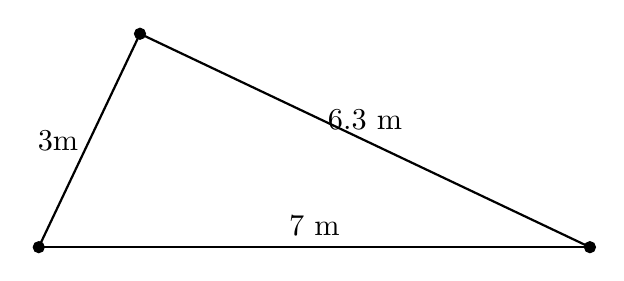
\begin{tikzpicture}
    \coordinate (a) at ({3 * cos(64.62)}, {3 * sin(64.62)});
    \filldraw [black] (7,0) circle (2pt);
    \filldraw [black] (0,0) circle (2pt);
    \draw [black,thick] (0,0) -- (a) node [midway, anchor=east] {3m};
    \draw [black,thick] (0,0) -- (7,0) node [midway, anchor=south] {7 m};
    \draw [black,thick] (7,0) -- (a) node [midway, anchor=south] {6.3 m};
    \filldraw [black] (a) circle (2pt);
  \end{tikzpicture}

  
  A right triangle with legs of 3m and 6.3m has an area of 9.45 square meters.

  There are two of them, so the total area is $36.27 + 2(18.9) = 74.07$ square meters.

  Six square meters per liter, so you need $\frac{74.07}{6} = 12.35$ liters of paint.

\end{Answer}

\graphicspath{{../../Chapters/functions/en_US}}
\chapter{Functions and Their Graphs}

You can think of a function as a machine: you put something into the
machine, it processes it, and out comes something else, a product. Just as we
often use the variable $x$ to stand in for a number, we often use the
variable $f$ to stand in for a function.
% One of my teachers told me half of understanding math is understanding mathmaticions are just lazy, maybe a good add in somewhere

For example, we might ask, ``Let the function $f$ be defined like this:

\begin{equation*}
f(x) = -5x^2 + 12x + 2
\end{equation*}

What is the value of $f(3)$?''

You would run the number 3 through ``the machine'': $-5(3^2) + 12(3) + 2 = -7$. The answer would be ``$f(3)$ is $7$''.

However, Some functions are not defined for every possible input. For example:

\begin{equation*}
  f(x) = \frac{1}{x}
\end{equation*}

  This is defined for any $x$ except 0, because you can't divide 1 by 0. The set of values that a function can process is called its \textit{domain}.

\begin{Exercise}[title={Domain of a function}, label=function_domain]

  Let the function $f$ be given by $f(x) = \sqrt{x - 3}$.  What is its domain?

\end{Exercise}
\begin{Answer}[ref=function_domain]
  You can only take the square root of nonnegative numbers, so the
  function is only defined when $x - 3 \geq 0$.  Thus the domain is
  all real numbers greater than or equal to 3.
\end{Answer}

\section{Graphs of Functions}

If you have a function, $f$, its graph is the set of pairs $(x, y)$
such that $y = f(x)$.  We usually draw a picture of this set, called a \textit{graph}. 
The graph not only includes the picture, but also the values of x and y used to create it.

Here is the graph of the function $f(x) = -5x^2 + 12x + 2$:

\begin{tikzpicture}
    \begin{axis}[
        xmin=-1,xmax=3.5,
        ymin=-10,ymax=11,
        axis x line=middle,
        axis y line=middle,
        axis line style=<->,
        xlabel={$x$},
        ylabel={$y$},
        ]
        \addplot[no marks,sdkblue,<->] expression[domain=-0.7:3.05,samples=100]{(-5)*(x^2) + (12 * x) + 2}; 
    \end{axis}
\end{tikzpicture}

(Note this is just part of the graph: it goes infinitely in both
directions, remember your vectors.)

Here is the graph of the function $f(x) = \frac{1}{x}$:

\begin{tikzpicture}
    \begin{axis}[
        xmin=-7,xmax=7,
        ymin=-7,ymax=7,
        axis x line=middle,
        axis y line=middle,
        axis line style=<->,
        xlabel={$x$},
        ylabel={$y$},
        ]
        \addplot[no marks,sdkblue,<->] expression[domain=-6.5:-0.15,samples=100]{1/x}; 
        \addplot[no marks,sdkblue,<->] expression[domain=0.15:6.5,samples=100]{1/x}; 
    \end{axis}
\end{tikzpicture}

\begin{Exercise}[title={Draw a graph}, label=draw_graph]

  Let the function $f$ be given by $f(x) = -3x + 3$. Sketch its graph.
% More space needed in exercise box
\end{Exercise}
\begin{Answer}[ref=draw_graph]

  The graph of this function is a line. Its slope is -3.  It intersects the y axis at $(0, 3)$

\begin{tikzpicture}
    \begin{axis}[
        xmin=-1,xmax=3,
        ymin=-7,ymax=7,
        xtick={1},
        ytick={3},
        axis x line=middle,
        axis y line=middle,
        axis line style=<->,
        xlabel={$x$},
        ylabel={$y$},
        ]
        \addplot[no marks,sdkblue,<->] expression[domain=-0.75:2.74,samples=100]{-3 * x + 3}; 
    \end{axis}
\end{tikzpicture}
  
  
\end{Answer}


\section{Can this be expressed as a function?}

Note that not all sets can be expressed as graphs of functions.  For
example, here is the set of points $(x,y)$ such that $x^2 + y^2 = 9$:

\begin{tikzpicture}
    \begin{axis}[
        xmin=-3.5,xmax=3.5,
        ymin=-3.5,ymax=3.5,
        ytick={-3,-2,-1,0,1,2,3},
        axis x line=middle,
        axis y line=middle,
        axis line style=<->,
        xlabel={$x$},
        ylabel={$y$},
        ]
        \addplot[no marks,sdkblue] expression[domain=-3:3,samples=100]{sqrt(9 - x^2)}; 
        \addplot[no marks,sdkblue] expression[domain=-3:3,samples=100]{-1 * sqrt(9 - x^2)}; 
    \end{axis}
\end{tikzpicture}

This cannot be the graph of a function because what would $f(0)$ be? 3
or -3?  This set fails what we call ``the vertical line test'': If any
vertical line contains more than one point from the set, it isn't the graph
of a function.  For example, the vertical line $x = 2$ would cross
the graph twice:
% index vertical line test
\begin{tikzpicture}
    \begin{axis}[
        xmin=-3.5,xmax=3.5,
        ymin=-3.5,ymax=3.5,
        ytick={-3,-2,-1,0,1,2,3},
        axis x line=middle,
        axis y line=middle,
        axis line style=<->,
        xlabel={$x$},
        ylabel={$y$},
        ]
        \addplot[no marks,sdkblue] expression[domain=-3:3,samples=100]{sqrt(9 - x^2)}; 
        \addplot[no marks,sdkblue] expression[domain=-3:3,samples=100]{-1 * sqrt(9 - x^2)};
        \addplot [thick, dashed] coordinates {(2,-2.5)(2,2.5)};

    \end{axis}

\end{tikzpicture}
% include linked exercise: https://youtu.be/xSQFPbhT4Yc


\section{Inverses}

Some functions have inverse functions. If a function $f$ is a machine that turns
number $x$ into $y$, the inverse (usually denoted $f^{-1}$) is the machine that turns $y$ back
into $x$.

For example, let $f(x) = 5x + 1$. Its inverse is
$f^{-1}(x) = (x - 1)/5$. (Spot check it: $f(3) = 16$ and $f^{-1}(16) = 3$)

Does the function $f(x) = x^3$ have an inverse? Yes, $f^{-1}(x) =
\sqrt[3]{x}$. Let's plot the function (solid line) and its inverse (dashed):

\begin{tikzpicture}
    \begin{axis}[
        xmin=-3.5,xmax=3.5,
        ymin=-3.5,ymax=3.5,
        ytick={-3,-2,-1,0,1,2,3},
        axis x line=middle,
        axis y line=middle,
        axis line style=<->,
        xlabel={$x$},
        ylabel={$y$},
        ]
        \addplot[no marks,sdkblue] expression[domain=-3:3,samples=100]{x^3}; 
        \addplot[no marks,sdkblue,dashed] expression[domain=0:3,samples=100]{x^(1/3)}; 
        \addplot[no marks,sdkblue,dashed] expression[domain=-3:0,samples=100]{-1 * (-1 * x)^(1/3)}; 
    \end{axis}
\end{tikzpicture}

The inverse is the same as the function, just with its axes swapped.
This tells us how to solve for an inverse: We swap $x$ and $y$ and
solve for $y$.

For example, if you are given the function $f(x) = 5x + 1$, its graph
is all $(x,y)$ such that $y = 5x + 1$.  The graph of its inverse is
all $(x, y)$ such that $x = 5y + 1$. So you solve for $y$: $y = (x -
1)/5$.

Not every function has an inverse.  For example, $f(x) = x^2$.  Note
that $f(2) = f(-2) = 4$.  What would $f^{-1}(4)$ be? 2 or -2?  This
implies the ``horizontal line test'': If any horizontal line contains
more than one point of a function's graph, that function has no
inverse.
% index horizontal line test
\begin{tikzpicture}
    \begin{axis}[
        xmin=-3.5,xmax=3.5,
        ymin=-1, ymax=6,
        ytick={-1,0,1,2,3,4,5,6},
        axis x line=middle,
        axis y line=middle,
        axis line style=<->,
        xlabel={$x$},
        ylabel={$y$},
        ]
      \addplot[no marks,sdkblue] expression[domain=-3:3,samples=100]{x^2};
      \addplot [thick, dashed] coordinates {(-3,4)(3,4)};
    \end{axis}
\end{tikzpicture}

In some problems, you need an inverse and you don't  need the
whole domain, so you trim the domain to a set you can define an
inverse on. This allow you to make claims such as ``If we restrict the domain to
the nonnegative numbers, the function $f(x) = x^2 - 5$ has an inverse:
$f^{-1}(x) =\sqrt{x + 5}$.

This begs the question: What is the domain of the inverse function $f^{-1}$?

If we let $X$ be the domain of $f$, we can run every member of $X$
through ``the machine'' and gather them in a set on the other
side. This set would be the \textit{image} of the $f$ "machine". (This is the \textit{range} of $f$.)

What is the image of $f(x) = x^2 - 5$? It is the set of all real
numbers greater than or equal to -5. We write this

\begin{equation*}
  \{ x \in {\rm I\!R} | x \geq -5 \}
  \end{equation*}

Now we can say: \textbf{The image of the function is the domain
  of the inverse function.}

In our example, we can use any number greater
than or equal to -5 as input into the inverse function.

\begin{tikzpicture}
    \begin{axis}[
        xmin=-5.5,xmax=7.5,
        ymin=-6, ymax=5,
        xtick={-3, 2},
        ytick={-5, 1},
        axis x line=middle,
        axis y line=middle,
        axis line style=<->,
        ]
      \addplot[no marks,sdkblue, ->] expression[domain=0:3,samples=100]{x^2 - 5} node[right] {$y = x^2 - 5$};
      \addplot [thick, dashed, red, ->] coordinates {(-0.05,-5)(-0.05,4.5)}
      node [draw, red, left, align=left, yshift=-0.6cm, xshift=-0.1cm] {image of $f$ \textit{or}\\ domain of $f^{-1}$};
      \addplot [thick, dashed, blue, ->] coordinates {(-0,-5.1)(6.75,-5.1)}
      node [draw, align=left, above, blue, yshift=0.1cm, xshift=-1.3cm] {domain of $f$ \textit{or}\\image of $f^{-1}$};
    \end{axis}
\end{tikzpicture}


\begin{Exercise}[title={Find the inverse}, label=simple_inverse]

  Let $f(x) = (x - 3)^2 + 2$.  Sketch the graph.

  Using all the real numbers as a domain, does this function have an inverse?

  How would you restrict the domain to make the function invertible?

  What is the inverse of that restricted function?

  What is the domain of the inverse?

\end{Exercise}
\begin{Answer}[ref=simple_inverse]

  This graph is the graph of $y = x^2$ that has been moved to the right by three units and up two units:
 
\begin{tikzpicture}
    \begin{axis}[
        xmin=-1,xmax=7,
        ymin=-1,ymax=7,
        xtick={3, 6},
        ytick={2, 4},
        axis x line=middle,
        axis y line=middle,
        axis line style=<->,
        xlabel={$x$},
        ylabel={$y$},
        ]
      \addplot[no marks,sdkblue,<->] expression[domain=-2.5:6.5,samples=100]{(x - 3)^2 + 2};
      \addplot[dashed] coordinates {(-1, 2)(4,2)};
      \addplot[dashed] coordinates {(3, -1)(3, 3)};
    \end{axis}
\end{tikzpicture}

To prevent any horizontal line from containing more than one point of
the graph, you would need to use the left or the right side: Either
$\{x \in {\rm I\!R}  | x \leq 3\}$ or $\{x {\rm I\!R}| x \geq 3\}$. Most people will choose the
right side; the rest of the solution will assume that you did too.

To find the inverse we swap $x$ and $y$: $x = (y -3)^2 + 2$

The we solve for $y$ to get the inverse: $y = \sqrt{x - 2} + 3$

You can take the square root of nonnegative numbers. So the function
$f^{-1}(x) = \sqrt{x - 2} + 3$ is defined whenever $x$ is greater than
or equal to 2.

\end{Answer}

\section{Graphing Calculators}

One really easy way to understand your function better is to use a graphing
calculator. Desmos is a great, free online graphing calculator. 

In a web browser, go to Desmos: \url{https://www.desmos.com/calculator}

In the field on the left, enter the function $y = x^2 - x - 6$. (For
the exponent, just prefix it with a caret symbol: ``x\^2''.)

\includegraphics[width=0.85\textwidth]{Desmos.png}

\graphicspath{{../../Chapters/volume_solids/en_US}}
\chapter{Volumes of Common Solids}


The volume of a rectangular solid is the product of its three
dimensions.  So if a block of ice is 5 cm tall, 3 cm wide and, 2 cm
deep, it's volume is $5 \times 3 \times 2 = 30$ cubic centimeters.

\tdplotsetmaincoords{80}{130} 
\begin{tikzpicture} [scale=1, tdplot_main_coords, axis/.style={->,sdkblue}, 
light vector/.style={-stealth,dashed,very thick, black}, 
vector/.style={-stealth,black,very thick}, 
vector guide/.style={dashed,sdkblue}]

%standard tikz coordinate definition using x, y, z coords
\coordinate (O) at (0,0,0);

%draw axes
\draw[axis] (0,0,0) -- (3,0,0) node[anchor=north east]{$x$};
\draw[axis] (0,0,0) -- (0,4,0) node[anchor=north west]{$y$};
\draw[axis] (0,0,0) -- (0,0,5.2) node[anchor=south]{$z$};

%draw a vector from O to P
\draw[thick,black] (0,0,0) -- (0,0,5);
\draw[thick,black] (0,3,5) -- (0,0,5);
\draw[thick,black] (2,0,5) -- (0,0,5);

\draw[thick,black] (0,0,0) -- (0,3,0);
\draw[thick,black] (0,3,5) -- (0,3,0) node[midway, right]{$5$ cm};
\draw[thick,black] (2,3,0) -- (0,3,0) node[midway, below]{$2$ cm};;

\draw[thick,black] (0,0,0) -- (2,0,0);
\draw[thick,black] (2,0,5) -- (2,0,0);
\draw[thick,black] (2,3,0) -- (2,0,0) node[midway,below]{$3$ cm};

\draw[thick,black] (2,3,5) -- (2,0,5);
\draw[thick,black] (2,3,5) -- (0,3,5);
\draw[thick,black] (2,3,5) -- (2,3,0);

\end{tikzpicture}


A
cubic centimeter is the same as a milliliter. A milliliter of ice
weighs about 0.92 grams.  So the block of ice would have a mass of $30
\times 0.92 = 27.6$ grams. \index{volume ! rectangular solid}

\begin{mdframed}[style=important, frametitle={Volume of a Sphere}]

A sphere with a radius of $r$ has a volume of \index{volume ! sphere}

$$v = \frac{4}{3} \pi r^3$$

(For completeness, the surface area of that sphere would be

$$a  = 4 \pi r^2$$

Note that a circle of radius $r$ is one quarter of ths: $\pi r^2$.)

\end{mdframed}

\begin{Exercise}[title={Flying Sphere}, label=flying_sphere]

An iron sphere is traveling at 5 m/s. (It is not spinning.)  The
sphere has a radius of 1.5 m.  Iron has a density of 7,800 kg per
cubic meter.  How much kinetic energy does the sphere have?
\end{Exercise}
\begin{Answer}[ref=flying_sphere]
  The volume of the sphere (in cubic meters) is

  $$\frac{4}{3}\pi (1.5)^3 = 4.5 \pi \approx 14.14$$

  The mass (in kg) is $14.14 \times 7800 \approx 110,269$

  The kinetic energy (in joules) is

  $$k = \frac{110269 \times 5^2}{2} = 1,378,373$$

  About 1.4 million joules.
\end{Answer}

\section{Cylinders}

The base and the top of a right cylinder are identical circles. The
circles are on parallel planes.  The sides are perpendicular to those
planes.

\tdplotsetmaincoords{75}{0} 
\begin{tikzpicture} [scale=4, tdplot_main_coords, axis/.style={->,sdkblue}]
\draw[dashed, sdkblue] (0.5,0,0) -- (0.5,0,0.7) node[midway, right]{$h$};
\draw[dashed, sdkblue] (0.5,0,0) -- (1,0,0) node[midway, below]{$r$};
\draw[black] (0.5, 0, 0) circle (0.5);
\draw[black] (0.5, 0, 0.7) circle (0.5);
\draw[black] (0,0,0) -- (0,0,0.7);
\draw[black] (1,0,0) -- (1,0,0.7);
\draw[black] (0.5,0,0) circle (0.02);
\draw[black] (0.5,0,0.7) circle (0.02);
\end{tikzpicture}

\begin{mdframed}[style=important, frametitle={Volume of a cylinder}]\index{volume ! right cylinder}


The volume of the a right cylinder of radius $r$ and height
$h$ is given by:

$$v = \pi r^2 h$$

That is, it is the area of the base times the height.

\end{mdframed}

\begin{Exercise}[title={Tablet}, label=tablet]

  A drug company has to create a tablet with volume of 90 cubic millimeters.

  The tablet will be a cylinder with half spheres on each end.  The radius will be 2mm.

  How long do they need to make the tablet to be?

  \vspace{2mm}
  
\tdplotsetmaincoords{90}{20} 
\begin{tikzpicture} [scale=6.5, tdplot_main_coords, axis/.style={->,sdkblue}]
\draw[dashed, sdkblue] (-0.2,0,0) -- (0,0,0);
\draw[dashed, sdkblue] (0,0,0) -- (0,0,0.2) node[midway, right]{2 mm};
\draw[dashed, sdkblue] (0, 0, 0) [x={(0,0,1)}] circle (0.2);
\draw[dashed, sdkblue] (0.5, 0, 0) [x={(0,0,1)}] circle (0.2);
\draw[dashed, sdkblue] (0.5,0,0) -- (0.7,0,0);
\draw[black] (0, 0, -0.2) [y={(0,0,-1)}] arc (90:270:0.2);
\draw[black] (0.5, 0, 0.2) [y={(0,0,-1)}] arc (-90:90:0.2);
\draw[black] (0,0,0.2) -- (0.5,0,0.2);
\draw[black] (0,0,-0.2) -- (0.5,0,-0.2);
\draw[dashed, sdkblue] (-0.2, 0, 0) -- (-0.2, 0, -0.3);
\draw[dashed, sdkblue] (0.7, 0, 0) -- (0.7, 0, -0.3);
\draw[dashed, sdkblue] (-0.2, 0, -0.3) -- (0.7, 0, -0.3) node[midway, below]{?};
\end{tikzpicture}
  

\end{Exercise}
\begin{Answer}[ref=tablet]
  In your mind, you can dissemble the tablet into a sphere (made up of
  the two ends) and a cylinder (between the two ends)
  
  The volume of the sphere (in cubic millimeters) is

  $$\frac{4}{3}\pi (2)^3 =\frac{32}{3}\pi \approx 33.5$$

  Thus the cylinder part has to be $90 - 33.5 = 56.5$ cubic mm. The
  cylinder part has a radius of 2 mm. If the length of the cylinder
  part is $x$, then

  $$\pi 2^2 x = 56.5$$

  Thus $x = \frac{56.5}{4 \pi} \approx 4.5$ mm.

  The cylinder part of the table needs to be 4.5mm.  Thus the entire tablet is 8.5mm long.
  
\end{Answer}

What if the base and top are identical, but the sides aren't
perpendicular to the base? This is called \newterm{oblique cylinder}.

\tdplotsetmaincoords{75}{0} 
\begin{tikzpicture} [scale=4, tdplot_main_coords, axis/.style={->,sdkblue}]
\draw[dashed, sdkblue] (0.7,0,0) -- (0.7,0,0.7) node[midway, right]{$h$};
\draw[dashed, sdkblue] (0.5,0,0) -- (1,0,0) node[midway, below]{$r$};
\draw[black] (0.5, 0, 0) circle (0.5);
\draw[black] (0.7, 0, 0.7) circle (0.5);
\draw[black] (0,0,0) -- (0.2,0,0.7);
\draw[black] (1,0,0) -- (1.2,0,0.7);
\draw[black] (0.5,0,0) circle (0.02);
\draw[black] (0.7,0,0.7) circle (0.02);
\end{tikzpicture}

The volume is still the height times the area of the base.  Note,
however, that the height is measured perpendicular to the bottom and
top. \index{volume ! oblique cylinder}

Why?


\section{Volume, Area, and Height}

On a solid with a flat base, the line that we use to measure height is
always perpendicular to the plane of the base. We can take slices
through the solid that are parallel to that base plane.  For example,
if we have a pyramid with a square base, each slice will be a square
-- small squares near the top, larger squares near the bottom.

\tdplotsetmaincoords{80}{17} 
\begin{tikzpicture} [scale=4, tdplot_main_coords, axis/.style={->,sdkblue}]
  
\draw[dashed, sdkblue] (0.5,0.5,0) -- (0.5,0.5, 1.0) node[midway, right]{$h$};

\draw[black] (0,0,0) -- (0.5,0.5,1.0);
\draw[black] (1,0,0) -- (0.5,0.5,1.0);
\draw[black] (0,1,0) -- (0.5,0.5,1.0);
\draw[black] (1,1,0) -- (0.5,0.5,1.0);

\draw[black] (0,0,0) -- (1,0,0);
\draw[black] (0,0,0) -- (0,1,0);
\draw[black] (1,0,0) -- (1,1,0)node[midway,below]{$w$};
\draw[black] (0,1,0) -- (1,1,0);

\fill[sdkblue,,opacity=0.4] (0.125, 0.125, 0.25) -- (0.875, 0.125, 0.25) -- (0.875, 0.875, 0.25) -- (0.125, 0.875, 0.25);

\draw[dashed,sdkblue] (0.125, 0.125, 0.25) -- (0.875, 0.125, 0.25);
\draw[dashed,sdkblue] (0.125, 0.125, 0.25) -- (0.125, 0.875, 0.25);
\draw[dashed,sdkblue] (0.875, 0.125, 0.25) -- (0.875, 0.875, 0.25);
\draw[dashed,sdkblue] (0.125, 0.875, 0.25) -- (0.875, 0.875, 0.25);

\draw[dashed,sdkblue] (-0.1, -0.1, 0.25) -- (1.1, -0.1, 0.25);
\draw[dashed,sdkblue] (-0.1, -0.1, 0.25) -- (-0.1, 1.1, 0.25);
\draw[dashed,sdkblue] (1.1, -0.1, 0.25) -- (1.1, 1.1, 0.25);
\draw[dashed,sdkblue] (-0.1, 1.1, 0.25) -- (1.1, 1.1, 0.25);

\end{tikzpicture}

We can figure out the area of the slice at every height $z$.  For
example, at $z = 0$ the slice would have area $w^2$.  At $z = h$, the
slice would have zero area.  What about an arbitrary $z$ in between?
The edge of the square would be $w (1 - \frac{z}{h})$.  So the area of
the slice would be $w^2 (1 - \frac{z}{h})^2$

The graph of this would look like this:

\begin{tikzpicture}[scale=5]

\draw [sdkblue,->,thick] (0,0) -- (1.1,0) node[right]{$z$};
\draw [sdkblue,->,thick] (0,0) -- (0,1.1) node[above]{slice area};
\draw [sdkblue,dashed] (1, 1) -- (0,1) node[left] {$w^2$};
\draw [sdkblue,dashed] (1, 1) -- (1,0) node[below] {$h$};
 \fill [sdkblue, opacity=0.4, domain=0:1, variable=\x]
      (0, 0) 
      -- plot ({\x}, {(1.0 - \x)^2})
      -- (1, 0)
      -- cycle;
\draw[thick,draw=black,
      domain=0:1,samples=300,variable=\x] 
      plot (\x,{(1.0 - \x)^2});
\end{tikzpicture}

The volume is given by the area under the curve and above the
axis. Once you learn integration, you will be really good at finding
the area under the curve.  In this case, I will just tell you that in
the picture, the colored region is one third of the rectangle.

Thus, the area of a square-based pyramid is $\frac{1}{3} h w^2$.

In fact:

\begin{mdframed}[style=important, frametitle={Volume of a pyramid}]\index{volume ! pyramid}

  The volume of pyramid whose base has an area of $b$ and height $h$ is given by:

  $$V = \frac{1}{3} h b$$

  Regardless of the shape of the base.
\end{mdframed}

Note that this is true even for oblique pyramids:

\tdplotsetmaincoords{80}{30} 
\begin{tikzpicture} [scale=4, tdplot_main_coords, axis/.style={->,sdkblue}]
  
\draw[dashed, sdkblue] (1.6,0.5,0) -- (1.6,0.5, 1.0) node[midway, right]{$h$};
\fill[sdkblue] (1.6, 0.5, 0) circle (.02);

\draw[black] (0,0,0) -- (1.6,0.5,1.0);
\draw[black] (1,0,0) -- (1.6,0.5,1.0);
\draw[black] (0,1,0) -- (1.6,0.5,1.0);
\draw[black] (1,1,0) -- (1.6,0.5,1.0);

\draw[black] (0,0,0) -- (1,0,0);
\draw[black] (0,0,0) -- (0,1,0);
\draw[black] (1,0,0) -- (1,1,0);
\draw[black] (0,1,0) -- (1,1,0);

\fill[sdkblue,opacity=0.4] (0.4, 0.125, 0.25) -- (1.15, 0.125, 0.25) -- (1.15, 0.875, 0.25) -- (0.4, 0.875, 0.25);

\draw[dashed,sdkblue] (0, -0.1, 0.25) -- (1.3, -0.1, 0.25);
\draw[dashed,sdkblue] (0, -0.1, 0.25) -- (0, 1.1, 0.25);
\draw[dashed,sdkblue] (1.3, -0.1, 0.25) -- (1.3, 1.1, 0.25);
\draw[dashed,sdkblue] (0, 1.1, 0.25) -- (1.3, 1.1, 0.25);

\end{tikzpicture}


\begin{Exercise}[title={Hexagon-based Pyramid}, label=pyramid_volume]

There is a pyramid with a regular hexagon for a base. Each edge is 5 cm long.  The pyramid is 13 cm tall.  What is its volume?

\tdplotsetmaincoords{70}{17} 
\begin{tikzpicture} [scale=.5, tdplot_main_coords]
  
\draw[dashed, sdkblue] (0,0,0) -- (0,0,13) node[right]{13 cm};

\draw[black] (-5,0,0) -- (-2.5,4.33,0) -- (2.5,4.33,0) -- (5,0,0)
-- (2.5, -4.33, 0) -- (-2.5, -4.33,0) -- cycle;

\draw[black] (0, -4.5, 0) node {5 cm};

\draw[black] (-5,0,0) -- (0,0,13);
\draw[black] (0,0,13)--(5,0,0);
\draw[black] (-2.5,4.33,0) -- (0,0,13);
\draw[black] (2.5,4.33,0) -- (0,0,13);
\draw[black] (-2.5,-4.33,0) -- (0,0,13);
\draw[black] (2.5,-4.33,0) -- (0,0,13);
\end{tikzpicture}

\end{Exercise}
\begin{Answer}[ref=pyramid_volume]
  First, you need to find the area of the base, which is a regular hexagon:
  
\begin{tikzpicture}[scale=0.5]
  \draw[black] (-5,0) -- (-2.5,4.33) -- (2.5,4.33) -- (5,0)
-- (2.5, -4.33) -- (-2.5, -4.33) -- cycle node[midway,left]{5 cm};
\draw[sdkblue,dashed] (-5,0) -- (0,0);
\draw[sdkblue,dashed] (5,0) -- (0,0);
\draw[sdkblue,dashed] (-2.5,4.33) -- (0,0);
\draw[sdkblue,dashed] (2.5,4.33) -- (0,0);
\draw[sdkblue,dashed] (-2.5,-4.33) -- (0,0);
\draw[sdkblue,dashed] (2.5,-4.33) -- (0,0);
\end{tikzpicture}

All the angles in this picture are $60^\circ$ or $\frac{\pi}{3}$
radians. Thus, each line is 5 cm long.

Thus, we need to find the area of one of these triangles and multiply that by six.

Every triangle has a base of 5cm. How tall are they?

\begin{tikzpicture}
  \draw[black] (-2.5,0) -- (2.5,0) -- (0,4.33) -- cycle node[midway,left]{5 cm};
  \draw[sdkblue,dashed] (0,0) -- (0,4.33) node[midway,right]{?};
  \draw[black] (-2.0, 0.0) node [right, above] {$60^\circ$};
\end{tikzpicture}

$$5 \sin{60^\circ} = 5\frac{\sqrt{3}}{2}$$

Which is about 4.33 cm.

Thus, the area of single triangle is 

$$\frac{1}{2} (5) \left( 5\frac{\sqrt{3}}{2} \right) = 25 \frac{\sqrt{3}} {4}$$

And the area of the whole hexagon is six times that:

$$75 \frac{\sqrt{3}}{2}$$

Thus, the volume of the pyramid is:

$$\frac{1}{3}h b = \frac{1}{3} 13 \left(75 \frac{\sqrt{3}}{2}\right)$$

About 281.46 cubic centimeters.

\end{Answer}

Note that plotting the area of each slice and finding the area under
the curve will let you find the area of many things.  For example,
let's say that you have a four-sided spiral, where each face has the
same width $w$:

\tdplotsetmaincoords{80}{17} 
\begin{tikzpicture} [scale=4, tdplot_main_coords, axis/.style={->,sdkblue}]

  \def\h{1.570796326794897}
  \def\gap{0.2}
  \def\srad{0.707106781186548}

\fill[sdkblue,opacity=.7] (0,-1,0) -- (-1,0,0) -- (0,1,0) -- (1,0,0) -- cycle;

\draw[black,thick] (0,-1,0) -- (-1,0,0) -- (0,1,0) -- (1,0,0) -- cycle;
\draw[black,thick] (0,-1,\h) -- (-1,0,\h) -- (0,1,\h) -- (1,0,\h) -- cycle;

\foreach \x in {0.0, 0.1, 0.2, 0.3, 0.4, 0.5, 0.6, 0.7, 0.8, 0.9, 1.0, 1.1, 1.2, 1.3, 1.4, 1.5}{
%        \fill[sdkblue, opacity=0.3] ({sin(deg(\x) + 0)},{cos(deg(\x)+ 0)},\x) -- ({sin(deg(\x) + 90)},{cos(deg(\x)+ 90)},\x) --
%        ({sin(deg(\x + \gap) + 90)},{cos(deg(\x + \gap) + 90)},\x + \gap) -- ({sin(deg(\x + \gap) + 0},{cos(deg(\x + \gap)+ 0)},\x + \gap) -- cycle;
        
%        \fill[gray, opacity=0.8] ({sin(deg(\x) + 90)},{cos(deg(\x)+ 90)},\x) -- ({sin(deg(\x) + 180)},{cos(deg(\x)+ 180)},\x) --
%        ({sin(deg(\x + \gap) + 180)},{cos(deg(\x + \gap)+ 180)},\x + \gap) -- ({sin(deg(\x + \gap) + 90)},{cos(deg(\x + \gap)+ 90)},\x + \gap) -- cycle;
        
%        \fill[sdkblue,opacity=0.3] ({sin(deg(\x) + 180)},{cos(deg(\x)+ 180)},\x) -- ({sin(deg(\x) + 270)},{cos(deg(\x)+ 270)},\x) --
%        ({sin(deg(\x + \gap) + 270)},{cos(deg(\x + \gap)+ 270)},\x+\gap) -- ({sin(deg(\x + \gap) + 180)},{cos(deg(\x + \gap)+ 180)},\x + \gap) -- cycle;
        
%        \fill[gray] ({sin(deg(\x) + 270)},{cos(deg(\x)+ 270)},\x) -- ({sin(deg(\x) + 0)},{cos(deg(\x)+ 0)},\x) --
  %        ({sin(deg(\x + \gap) + 0)},{cos(deg(\x + \gap)+0)},\x + \gap) -- ({sin(deg(\x + \gap) + 270)},{cos(deg(\x + \gap)+ 270)},\x +\gap) -- cycle;

  \draw[sdkblue] ({sin(deg(\x) + 0)},{cos(deg(\x)+ 0)},\x) -- ({sin(deg(\x) + 90)},{cos(deg(\x)+ 90)},\x) --
  ({sin(deg(\x) + 180)},{cos(deg(\x)+ 180)},\x) -- ({sin(deg(\x) + 270)},{cos(deg(\x)+ 270)},\x);
      }

\draw[thick,draw=black,
      domain=0:\h,samples=100,variable=\x] 
      plot ({sin(deg(\x) + 0)},{cos(deg(\x)+ 0)}, \x);

\draw[dashed,draw=sdkblue,
      domain=0:\h,samples=100,variable=\x] 
      plot ({\srad * sin(deg(\x) + 45)},{\srad * cos(deg(\x)+ 45)}, \x);

\draw[thick,draw=black,
      domain=0:\h,samples=100,variable=\x] 
      plot ({sin(deg(\x) + 90)},{cos(deg(\x)+ 90)}, \x);
\draw[dashed,draw=sdkblue,
      domain=0:\h,samples=100,variable=\x] 
      plot ({\srad * sin(deg(\x) + 135)},{\srad * cos(deg(\x)+ 135)}, \x);
      
\draw[thick,draw=black,
      domain=0:\h,samples=100,variable=\x] 
      plot ({sin(deg(\x) + 180)},{cos(deg(\x) + 180)}, \x);
%\draw[dashed,draw=sdkblue,
%      domain=0:\h,samples=100,variable=\x] 
%      plot ({\srad * sin(deg(\x) + 225)},{\srad * cos(deg(\x)+ 225)}, \x);

      
\draw[dashed, thick,draw=black,
      domain=0:\h,samples=100,variable=\x] 
      plot ({sin(deg(\x) + 270)},{cos(deg(\x) + 270)}, \x);

%\draw[dashed,draw=sdkblue,
%      domain=0:\h,samples=100,variable=\x] 
%      plot ({\srad * sin(deg(\x) + 315)},{\srad * cos(deg(\x)+ 315)}, \x);


      \fill[sdkblue,opacity=.9] (0,-1,\h) -- (-1,0,\h) -- (0,1,\h) -- (1,0,\h) -- cycle;
      \draw (0.7,-0.6,0) node [below] {$w$};
      \draw[dashed, sdkblue] (-1.1,0,0) -- (-1.1,0,\h) node[midway,left]{$h$};


\end{tikzpicture}

Every slice still has an area of $w^2$,  thus this figure has a volume of $h w^2$.


\begin{Exercise}[title={Volume of a building}, label=building_volume]

An architect is designing a hotel with a right triangular base; the base is 30
meters on each leg.  The building gets narrower as you get closer to
the top, and finally shrinks to a point.  The spine of the building is
where the right angle is. That spine is straight and perpendicular to the ground.

Each floor has a right isosceles triangle as its floor plan.  The
length of each leg is given by this formula:

$$w = 30 \sqrt{1 - \frac{z}{100}}$$

So the width of the building is 30 meters at height $z=0$.  At 100
meters, the building comes to a point.  It will like this:
\hspace{8mm}

\tdplotsetmaincoords{75}{120}
\begin{tikzpicture} [scale=1, tdplot_main_coords]
\def\h{10}
\draw[dashed, sdkblue] (0,3,0) -- (0,3.2,0) -- (0,3.2,\h) node[midway, right]{100m} -- (0,0,\h);

\draw[black] (0,0,0) -- (3,0,0) -- (0,3,0) -- cycle node [midway, above]{30m};
\draw[black] (0,0,0) -- (0,0,\h);
\draw[black] (0.5, 0, 0) -- (0.5, 0.5, 0) -- (0, 0.5, 0);
\draw[thick,draw=black,
      domain=0:\h,samples=100,variable=\x] 
      plot ({3 * sqrt(1 - (\x/\h)}, 0, \x);

\draw[thick,draw=black,
      domain=0:\h,samples=100,variable=\x] 
      plot (0, {3 * sqrt(1 - (\x/\h))}, \x);

\foreach \n in {1,...,\h}{
  \draw [dashed, draw=sdkblue] (0,0,\n) -- ({3 * sqrt(1 - \n/\h)}, 0, \n) -- (0, {3 * sqrt(1 - \n/\h)},\n) -- cycle;
  \draw [draw=sdkblue] (0.5,0,\n) -- (0.5, 0.5, \n) -- (0, 0.5,\n);
};
      
\end{tikzpicture}

What is the volume of the building in cubic meters?
\end{Exercise}
\begin{Answer}[ref=building_volume]

  The area at height $z$ is given by:

  $$a = \frac{1}{2} w^2 =\frac{1}{2} \left(30 \sqrt{1 - \frac{z}{100}}\right)^2 = \frac{1}{2} 900 \left(1 - \frac{z}{100}\right)$$

  If we plot that, it looks like this:

\begin{tikzpicture}
  \def\h{5}
  \draw[sdkblue, ->] (0,0) -- (0, \h + 0.5) node[above] {area};
  \draw[sdkblue, ->] (0,0) -- (3.5, 0) node[right] {$z$};
 \fill [sdkblue, opacity=0.4]
      (0, 0) -- (0,\h) node [left] {$900 m^2$} -- (3,0) node[below] {$100 m$} -- cycle;
\end{tikzpicture}

What is the area of the blue region? $\frac{1}{2} (900)(100) = 45,000$

The building will be 45 thousand cubic meters.


\end{Answer}

\graphicspath{{../../Chapters/conic_sections/en_US}}
\chapter{Conic Sections}

In mathematics, conic sections (or simply conics) are curves obtained as the intersection of the surface of a cone with a plane. The three types of conic section are the hyperbola, the parabola, and the ellipse; the circle is a special case of the ellipse, though historically it was sometimes called a fourth type.

\section{Definitions}

Each type of conic sections can be defined as follows:

\subsection{Circle}

A circle is the set of all points in a plane that are at a given distance (the radius) from a given point (the center). The standard equation for a circle with center $(h,k)$ and radius $r$ is:

\begin{equation}
(x - h)^2 + (y - k)^2 = r^2
\end{equation}

\subsection{Ellipse}

An ellipse is the set of all points such that the sum of the distances from two fixed points (the foci) is constant. The standard equation for an ellipse centered at the origin with semi-major axis $a$ and semi-minor axis $b$ is:

\begin{equation}
\frac{x^2}{a^2} + \frac{y^2}{b^2} = 1
\end{equation}

\subsection{Hyperbola}

A hyperbola is the set of all points such that the absolute difference of the distances from two fixed points (the foci) is constant. The standard equation for a hyperbola centered at the origin is:

\begin{equation}
\frac{x^2}{a^2} - \frac{y^2}{b^2} = 1
\end{equation}

or

\begin{equation}
\frac{y^2}{b^2} - \frac{x^2}{a^2} = 1
\end{equation}

depending on the orientation of the hyperbola.

\subsection{Parabola}

A parabola is the set of all points that are equidistant from a fixed point (the focus) and a fixed line (the directrix). The standard equation for a parabola that opens upwards or downwards is:

\begin{equation}
y = a(x - h)^2 + k
\end{equation}

and that opens leftwards or rightwards is:

\begin{equation}
x = a(y - k)^2 + h
\end{equation}

where $(h,k)$ is the vertex of the parabola.

\
\graphicspath{{../../Chapters/falling_bodies/en_US}}
\chapter{Falling Bodies}

Because of gravity, if you throw a hammer straight up in the air, from
the moment it leaves your hand until it hits the ground, it is
accelerating toward the center of the earth at a constant rate.

\includegraphics[width=1\textwidth]{hammerFall.png}

\emph{Acceleration} can be defined as change in velocity. If the hammer leaves your
hand with a velocity of 12 meters per second upward, one second later
it will be rising, and its velocity will have slowed to 2.2 meters per
second. One second after that, the hammer will be falling at a rate of
7.6 meters per second. Every second the hammer's velocity is changing by
9.8 meters per second, and that change is always toward the center of
the earth. When the hammer is going up, gravity is slowing it down by
9.8 meters per second, each second it is in the air.  When the hammer is coming down,
gravity is speeding it up by 9.8 meters per second.\index{acceleration}
% Connect to vectors


\includegraphics[width=.8\textwidth]{hammerTime.png}

Acceleration due to gravity on earth is a constant negative 9.8 meters per second per second:
\begin{equation*}
a = -9.8   
\end{equation*}
(Why is it negative? We are talking about height, which increases as
you go away from the center of the earth. Acceleration is changing the
velocity in the opposite direction.)

\section{Calculating the Velocity}

Given that the acceleration is constant, it makes sense that the
velocity is a straight line. Assuming once again that the hammer
leaves your hand at 12 meters per second, then the upwards velocity at
time $t$ is given by:
\begin{equation*}
  v = 12 - 9.8t
\end{equation*}

Note that the velocity of the hammer is being given as a function. Here is its graph:

\begin{tikzpicture}
    \begin{axis}[
        xmin=-0.25,xmax=2.75,
        ymin=-13,ymax=13,
        axis x line=middle,
        axis y line=middle,
        axis line style=<->,
        xlabel={$t$},
        ylabel={$v$},
        ]
        \addplot[no marks,sdkblue] expression[domain=0:2.25,samples=100]{x * (-9.8) + 12} node[left] {$12 - 9.8t$}; 
    \end{axis}
\end{tikzpicture}

\begin{Exercise}[title={When is the apex of flight?}, label=vapex]
  Given the hammer's velocity is given by $12 - 9.8t$, at what time (in seconds)
  does it stop rising and begin to fall?
\end{Exercise}
\begin{Answer}[ref=vapex]
  Solve for when the velocity is zero.

  $t = \frac{12}{9.8} = 1.22$ seconds after release.
\end{Answer}

At this point, we need to acknowledge air resistance. Gravity
is not the only force on the hammer; as it travels through the air,
the air tries to slow it down. This force is called \emph{air resistance},
and for a large, fast-moving object (like an airplane) it is GIGANTIC force. For a
dense object (like a hammer) moving at a slow speed (what you generate
with your hand), air resistance doesn't significantly affect acceleration.
% Relate to f=ma

\section{Calculating Position}

If you let go of the hammer when it is 2 meters
above the ground, the height of the hammer is given by:
\begin{equation*}
  p = -\frac{9.8}{2}t^2 + 12t + 2
\end{equation*}

Here is a graph of this function:

\begin{tikzpicture}
    \begin{axis}[
        xmin=-1.2,xmax=3.5,
        ymin=-13,ymax=13,
        axis x line=middle,
        axis y line=middle,
        axis line style=<->,
        xlabel={$t$},
        ylabel={$p$},
      ]
      \addplot[no marks,sdkblue,dashed,<-] expression [domain=-0.7:0,samples=100] {(-4.9)*(x^2) + 12 * x + 2};
      \addplot[no marks,sdkblue] expression [domain=0:2.58,samples=100] {(-4.9)*(x^2) + 12 * x + 2};
      \addplot[no marks,sdkblue,dashed,->] expression [domain=2.58:3,samples=100] {(-4.9)*(x^2) + 12 * x + 2};
    \end{axis}
\end{tikzpicture}


How do we know? \textbf{The change in position between time
  $0$ and any time $t$ is equal to the area under the velocity graph
  between $x = 0$ and $x = t$.}

Let's use the velocity graph to figure out how much the position has
changed in the first second of the hammer's flight. Here's the
velocity graph with the area under the graph for the first second filled
in:

\usepgfplotslibrary{fillbetween}

\begin{tikzpicture}
    \begin{axis}[
        xmin=-0.25,xmax=2.75,
        ymin=-13,ymax=13,
        axis x line=middle,
        axis y line=middle,
        axis line style=<->,
        xlabel={$t$},
        ylabel={$v$},
      ]
      \addplot[no marks,sdkblue, name path=f] expression[domain=0:2.25,samples=100]{x * (-9.8) + 12} node[left] {$12 - 9.8t$};
      \path[name path=xaxis] (axis cs:0,0) -- (axis cs:1,0);
      \addplot[
        thick,
        color=sdkblue,
        fill=sdkblue, 
        fill opacity=0.05
    ]
    fill between[
        of=f and xaxis,
        soft clip={domain=0:1},
    ];
    \addplot[dashed,gray] coordinates {(0,12)(1,12)};
    \addplot[dashed,gray] coordinates {(1,12)(1,0)};
    \end{axis}
\end{tikzpicture}

The blue filled region is the area of the dashed rectangle minus that
empty triangle in its upper left.  The height of the rectangle is
twelve and its width is the amount of time the hammer has been in
flight ($t$). The triangle is $t$ wide and $9.8t$ tall. Thus, the
area of the blue region is given by $12t - \frac{1}{2}9.8 t^2$.

That's the change in position. Where was it originally? 2 meters off
the ground. So the height is given by $p = 2 + 12t - \frac{1}{2}9.8t^2$.
We usually write terms so that the exponent decreases, so:

$$p = - \frac{1}{2}9.8t^2 + 12t + 2$$

Finding the area under the curve like this is called
\textit{integration}. We say ``To find a function that gives the
change in position, we just integrate the velocity function.''  A lot
of the study of calculus is learning to integrate different sorts of
functions.\index{integration}

One important note about integration: Any time the curve drops under
the $x$-axis, the area is considered negative. (Which makes sense,
right? If the velocity is negative, the hammer's position is
decreasing.)


\begin{tikzpicture}
    \begin{axis}[
        xmin=-0.25,xmax=2.75,
        ymin=-13,ymax=13,
        axis x line=middle,
        axis y line=middle,
        axis line style=<->,
        xlabel={$t$},
        ylabel={$v$},
      ]
      \addplot[no marks,sdkblue, name path=f] expression[domain=0:2.25,samples=100]{x * (-9.8) + 12} node[left] {$12 - 9.8t$};
      \path[name path=xaxis] (axis cs:0,0) -- (axis cs:2.25,0);
      \addplot[
        thick,
        color=sdkblue,
        fill=sdkblue, 
        fill opacity=0.05
      ]
      fill between[
        of=f and xaxis,
        soft clip={domain=0:1.2245},
      ];
      \addplot[
        thick,
        color=red,
        fill=red, 
        fill opacity=0.07
      ]
      fill between[
        of=f and xaxis,
        soft clip={domain=1.2245:2.1},
      ];
    \end{axis}
\end{tikzpicture}


\section{Quadratic functions}

Functions of the form $f(x) = a x^2 + b x + c$ are called \newterm{quadratic functions}. 
If $a > 0$, the ends go up.
If $a < 0$, the ends go down.\index{quadratic functions}


\begin{tikzpicture}
  \begin{axis}[
      xmin=-2.2,xmax=1.2,
      ymin=-2,ymax=3,
      axis x line=middle,
      axis y line=middle,
      axis line style=<->,
    ]
    \addplot[no marks,sdkblue] expression [domain=-2:1,samples=100] {(2)*(x^2) + 2 * x - 1};
  \end{axis}
  \node[right] at (1,4) {$2x^2 + 2x - 1$};
\end{tikzpicture}
\hspace{4mm}
\begin{tikzpicture}
  \begin{axis}[
    xmin=-1.5,xmax=1.5,
    ymin=-2,ymax=1.5,
    axis x line=middle,
    axis y line=middle,
    axis line style=<->,
  ]
  \addplot[no marks,sdkblue] expression [domain=-1.5:1.5,samples=100] {(-1.2)*(x^2) + 0.5 * x + 1};
\end{axis}
\node[right] at (0.5,1) {$-1.2 x^2 + 0.5 x + 1$};
\end{tikzpicture}

The graph of a quadratic function is a \newterm{parabola}.

\section{Simulating a falling body in Python}

Now you are going to write some Python code that simulates the flying hammer. First, we are just going to print out the position, speed, and acceleration of the hammer for every 1/100th of a second after it leaves your hand. (Later we will make a graph.)

Create a file called \filename{falling.py} and type this into it:

\begin{Verbatim}
# Acceleration on earth
acceleration = -9.8 # m/s/s

# Size of time step
time_step = 0.01 # seconds

# Initial values
speed = 12  # m/s upward
height = 2  # m above the ground
current_time = 0.0  # seconds after release

# Is the hammer still aloft?
while height > 0.0:

    # Show the values
    print(f"{current_time:.2f} s:")
    print(f"\tacceleration: {acceleration:.2f} m/s/s")
    print(f"\tspeed: {speed:.2f} m/s")
    print(f"\theight: {height:.2f} m")

    # Update height
    height = height + time_step * speed

    # Update speed
    speed = speed + time_step * acceleration

    # Update time
    current_time = current_time + time_step


print(f"Hit the ground: Complete")
\end{Verbatim}

When you run it, you will see something like this:
\begin{Verbatim}
0.00 s:
	acceleration: -9.80 m/s/s
	speed: 12.00 m/s
	height: 2.00 m
0.01 s:
	acceleration: -9.80 m/s/s
	speed: 11.90 m/s
	height: 2.12 m
0.02 s:
	acceleration: -9.80 m/s/s
	speed: 11.80 m/s
	height: 2.24 m
0.03 s:
	acceleration: -9.80 m/s/s
	speed: 11.71 m/s
	height: 2.36 m
...
2.60 s:
	acceleration: -9.80 m/s/s
	speed: -13.48 m/s
	height: 0.20 m
2.61 s:
	acceleration: -9.80 m/s/s
	speed: -13.58 m/s
	height: 0.07 m
Hit the ground: Complete
\end{Verbatim}

Note that the acceleration isn't changing at all, but it is changing
the speed, and the speed is changing the height.

We can see that the hammer in our simulation hits the ground just
after 2.61 seconds.

\subsection{Graphs and Lists}

Now, we are going to graph the acceleration, speed, and height using a
library called matplotlib. However, to make the graphs, we
need to gather all the data into lists.\index{matplotlib}

For example, we will have a list of speeds, and the first three
entries will be 12.0, 11.9, and 11.8.\index{lists, python}

We create an empty list and assign it to a variable like this:
\begin{Verbatim}
x = []
\end{Verbatim}

Then we can add items like this:
\begin{Verbatim}
x.append(3.14)
\end{Verbatim}

To get the first time back, we can ask for the object at index 0.
\begin{Verbatim}
y = x[0]
\end{Verbatim}
Note that the list starts at 0.  So if you have 32 items in the list,
the first item is at index 0. The last item is at index 31.

Duplicate the file \filename{falling.py} and name the new copy \filename{falling\_graph.py}

We are going to make a plot of the height over time. At the start of the program, you will import the
matplotlib library.  At the end of the program, you will create a plot and show it to the user.

In \filename{falling\_graph.py}, add the bold code:

\begin{Verbatim}[commandchars=\\\{\}]
\textbf{import matplotlib.pyplot as plt}

# Acceleration on earth
acceleration = -9.8 # m/s/s

# Size of time step
time_step = 0.01 # seconds

# Initial values
speed = 12  # m/s upward
height = 2  # m above the ground
current_time = 0.0  # seconds after release

\textbf{# Create empty lists}
\textbf{accelerations = []}
\textbf{speeds = []}
\textbf{heights = []}
\textbf{times = []}

# Is the hammer still aloft?
while height > 0.0:

    \textbf{# Add the data to the lists}
    \textbf{times.append(current_time)}
    \textbf{accelerations.append(acceleration)}
    \textbf{speeds.append(speed)}
    \textbf{heights.append(height)}
    
    # Update height
    height = height + time_step * speed

    # Update speed
    speed = speed + time_step * acceleration

    # Update time
    current_time = current_time + time_step

\textbf{# Make a plot}
\textbf{fig, ax = plt.subplots()}
fig.suptitle("Falling Hammer")
\textbf{ax.set_xlabel("Time (s)")}
\textbf{ax.set_ylabel("Height (m)")}
\textbf{ax.plot(times, heights)}
\textbf{plt.show()}
\end{Verbatim}

When you run the program, you should see a graph of the height over time.

\includegraphics[width=0.7\linewidth]{heightplot.png}

It is more interesting if we can see all three: acceleration, speed, and height. 
So lets make three stacked plots.  Change the plotting code in \filename{falling\_graph.py} to:\index{matplotlib!subplots}

\begin{Verbatim}
# Make a plot with three subplots
fig, ax = plt.subplots(3,1)
fig.suptitle("Falling Hammer")

# The first subplot is acceleration
ax[0].set_ylabel("Acceleration (m/s/s)")
ax[0].plot(times, accelerations)

# Second subplot is speed
ax[1].set_ylabel("Speed (m/s)")
ax[1].plot(times, speeds)

# Third subplot is height
ax[2].set_xlabel("Time (s)")
ax[2].set_ylabel("Height (m)")
ax[2].plot(times, heights)
plt.show()
\end{Verbatim}

Now you will get plots of all three variables:

\includegraphics[width=0.8\linewidth]{stackedplot.png}

This is what we expected, right?  The acceleration is a constant negative number.  The speed is a
straight line with a negative slope.  The height is a parabola.

A natural question at this point is ``When exactly will the hammer hit the
ground?''  That is, when does $height = 0$? The values of $t$ where a function is zero are
known as its \textit{roots}. Height is given by a quadratic function. In the next
chapter, you will get the trick for finding the roots of any quadratic
function.

\graphicspath{{../../Chapters/solving_quadratics/en_US}}
\chapter{Introduction to the Kontinua Sequence}

This book will start you on the long and difficult trek to becoming a modern
problem solver. Along the path, you will learn how to use the tools of
math, computers, and science.

Why should you bother? There are big problems in this world that will
require expert problem solvers. Those people will make the world a
better place while enjoying interesting and lucrative careers. We are
talking about engineers, scientists, doctors, computer programmers,
architects, actuaries, and mathematicians. Right now, those occupations represent
about 6\% of all the jobs in the United States. Soon,
that number is expected to rise above 10\%.  On average, people in
that 10\% of the population are expected to have salaries twice that
of their non-technical counterparts.\index{career}

Solving problems is difficult. At some point on this journey, you will
see people who are better at solving problems than you are. You, like
every other person who has gone on this journey, will think ``I have
worked so hard on this, but that person is better at it than
I am. I should quit.'' Don't.\index{quitting}

First, solving problems is like a muscle. The more you do, the better
you get at it.  It is OK to say ``I am not good at this yet.'' That
just means you need more practice.

Second, you don't need to be the best in the world. 10 million people
your age can be better at solving problems than you, \textit{and you
  can still be in the top 10\% of the world}. If you complete this
journey, there will be problems for you to solve and a job where your
problem-solving skills will be appreciated.

\emph{Where do we start?}

The famous physicist Richard Feynman once asked this question: ``If,
in some cataclysm, all of scientific knowledge were to be destroyed,
and only one sentence was passed on to the next generation of
creatures, what statement would contain the most information in the
fewest words?''

His answer was ``All things are made of atoms—little particles that move around in
perpetual motion, attracting each other when they are a little
distance apart, but repelling upon being squeezed into one another.''

\emph{That} seems like a good place to start.

\graphicspath{{../../Chapters/complex_numbers/en_US}}
\chapter{Complex Numbers}

Complex numbers are an extension of the real numbers, which in turn are an extension of the rational numbers. In mathematics, the set of complex numbers is a number system that extends the real number line to a full two dimensions, using the imaginary unit which is denoted by $i$, with the property that $i^2 = -1$.

\section{Definition}

A complex number is a number of the form $a + bi$, where $a$ and $b$ are real numbers, and $i$ is the imaginary unit, with the property that $i^2 = -1$. The real part of the complex number is $a$, and the imaginary part is $b$. 

\section{Why Are Complex Numbers Necessary?}

Complex numbers are essential to many fields of science and engineering. Here are a few reasons why:

\subsection{Roots of Negative Numbers}

In the real number system, the square root of a negative number does not exist because there is no real number that you can square to get a negative number. The introduction of the imaginary unit $i$, which has the property that $i^2 = -1$, allows us to take square roots of negative numbers and gives rise to complex numbers.

\subsection{Polynomial Equations}

The fundamental theorem of algebra states that every non-constant polynomial equation with complex coefficients has a complex root. This theorem guarantees that polynomial equations of degree $n$ always have $n$ roots in the complex plane.

\subsection{Physics and Engineering}

In physics and engineering, complex numbers are used to represent waveforms, in control systems, in quantum mechanics, and many other areas. Their properties make many mathematical manipulations more convenient.

\section{Adding Complex Numbers}

The addition of complex numbers is straightforward. If we have two complex numbers $z_1 = a + bi$ and $z_2 = c + di$, their sum is defined as:

\begin{equation}
z_1 + z_2 = (a + c) + (b + d)i
\end{equation}

In other words, you add the real parts to get the real part of the sum, and add the imaginary parts to get the imaginary part of the sum.

\section{Multiplying Complex Numbers}

The multiplication of complex numbers is a bit more involved. If we have two complex numbers $z_1 = a + bi$ and $z_2 = c + di$, their product is defined as:

\begin{equation}
z_1 \cdot z_2 = (a + bi) \cdot (c + di) = ac + adi + bci - bd = (ac - bd) + (ad + bc)i
\end{equation}

Note the last term comes from $i^2 = -1$. You multiply the real parts and the imaginary parts just as you would in a binomial multiplication, and remember to replace $i^2$ with $-1$.


\graphicspath{{../../Chapters/vectors/en_US}}
\chapter{Vectors}

We have talked a some about forces, but in the calculations that we
have done, we have only talked about the magnitude of a force. It is
equally important to talk about its direction. To do the math on
things with a magnitude and a direction (like forces), we need vectors.\index{vectors}

For example, if you jump out of a plane (hopefully with a parachute), 
several forces with different magnitudes and directions will be acting upon 
you. Gravity will push you straight down. That force will be proportional to your weight.
If there were a wind from the west, it would push you toward the east. That force
will be proportional to the square of the speed of the wind and approximately proportional to 
your size. Once you are falling, there will be resistance from the air 
that you are pushing through -- that force will point in the opposite direction
from the direction you are moving and will be proportional to the square of your
speed.
% Image needed

To figure out the net force (which will tell us how we will accelerate), we will 
need to add these forces together. So we need to learn to do math with vectors.

\section{Adding Vectors}

A vector is typically represented as a list of numbers, with each
number representing a particular dimension. For example, if I am
creating a 3-dimensional vector representing a force, it will have
three numbers representing the amount of force in each of the three
axes. For example, if a force of one newton is in the direction of the
$x$-axis, I might represent the vector as $v = [1, 0, 0]$. 
Another vector might be $u = [0.5, 0.9, 0.7]$ \index{vectors!adding}

\tdplotsetmaincoords{80}{130} 
\begin{tikzpicture} [scale=4, tdplot_main_coords, axis/.style={->,sdkblue}, 
vector/.style={-stealth,black,very thick}, 
vector guide/.style={dashed,sdkblue}]

%standard tikz coordinate definition using x, y, z coords
\coordinate (O) at (0,0,0);

%draw axes
\draw[axis] (0,0,0) -- (1.5,0,0) node[anchor=north east]{$x$};
\draw[axis] (0,0,0) -- (0,0.9,0) node[anchor=north west]{$y$};
\draw[axis] (0,0,0) -- (0,0,0.9) node[anchor=south]{$z$};

%draw a vector from O to P
\draw[vector] (O) -- (1,0,0);
\draw[vector] (O) -- (0.5,0.9,0.7);
\draw (0.2,0.0,0.05) node[left] {v};
\draw (0.2,0.35,0.3) node[right] {u};

\draw[vector guide] (0.5,0,0) -- (0.5,0.9,0);
\draw[vector guide] (0.0,0.9,0) -- (0.5,0.9,0);
\draw[vector guide] (0.5,0.9,0) -- (0.5,0.9,0.7);
\end{tikzpicture}

Thinking visually, when we add to vectors, we put the starting point 
second vector at the ending point of the first vector.


\tdplotsetmaincoords{80}{130} 
\begin{tikzpicture} [scale=4, tdplot_main_coords, axis/.style={->,sdkblue}, 
light vector/.style={-stealth,dashed,very thick, black}, 
vector/.style={-stealth,black,very thick}, 
vector guide/.style={dashed,sdkblue}]

%standard tikz coordinate definition using x, y, z coords
\coordinate (O) at (0,0,0);

%draw axes
\draw[axis] (0,0,0) -- (1.5,0,0) node[anchor=north east]{$x$};
\draw[axis] (0,0,0) -- (0,0.9,0) node[anchor=north west]{$y$};
\draw[axis] (0,0,0) -- (0,0,0.9) node[anchor=south]{$z$};

%draw a vector from O to P
\draw[light vector] (0,0,0) -- (0.5,0.9,0.7);
\draw[light vector] (0.5, 0.9, 0.7) -- (1.5, 0.9, 0.7);
\draw[vector] (0,0,0) -- (1.5,0.9,0.7) node[left] {u + v};
\draw (0.7,0.9,0.75) node[left] {v};
\draw (0.2,0.35,0.3) node[right] {u};

\draw[vector guide] (0.5,0,0) -- (0.5,0.9,0);
\draw[vector guide] (0.0,0.9,0) -- (0.5,0.9,0);
\draw[vector guide] (0.5,0.9,0) -- (0.5,0.9,0.7);
\draw[vector guide] (0.5,0.9,0) -- (1.5,0.9,0.0);
\draw[vector guide] (1.5,0.9,0.0) -- (1.5,0.9,0.7);
\draw[vector guide] (1.5,0.0,0.0) -- (1.5,0.9,0.0);

\end{tikzpicture}

If you know the vectors, you will just add them element-wise:

$$ u + v = [0.5, 0.9, 0.7] + [1.0, 0.0, 0.0] = [1.5, 0.9. 0.7] $$

These vectors have 3 components, so we say they are \newterm{3-dimensional}. 
Vectors can have any number of components. For example, the vector
 $[-12.2, 3, \pi, 10000]$ is 4-dimensional.

 You can only add two vectors if they have the same dimension.

 $$ [12, -4] + [-1, 5] = [11,1] $$

 Addition is commutative: If you have two vectors $a$ and $b$, then
 $a + b$ is the same as $b + a$.

 Addition is also associative: If you have three vectors $a$, $b$, and $c$,
 it doesn't matter which order you add them in. 
 That is, $a + (b + c) = (a + b) + c$.

 A 1-dimensional vector is just a number. We say it is a 
 \newterm{scalar}, not a vector.

 \begin{Exercise}[title={Adding vectors}, label=adding_vectors]
Add the following vectors:
\begin{itemize}
    \item $[1, 2, 3] + [4, 5, 6]$
    \item $[-1, -2, -3, -4] + [4, 5, 6, 7]$
    \item $[\pi, 0, 0] + [0, \pi, 0] + [0, 0, \pi]$
\end{itemize}
\end{Exercise}
\begin{Answer}[ref=adding_vectors]
    \begin{itemize}
        \item $[1, 2, 3] + [4, 5, 6] = [5, 7, 9]$
        \item $[-1, -2, -3, -4] + [4, 5, 6, 7] = [3, 3, 3, 3]$
        \item $[\pi, 0, 0] + [0, \pi, 0] + [0, 0, \pi] = [\pi, \pi, \pi]$ 
    \end{itemize}
\end{Answer}

    \begin{Exercise}[title={Adding Forces}, label=adding_forces]
        You are adrift in space. You are near two different stars. 
        The gravity of one star is pulling you towards it with a 
        force of $[4.2, 5.6, 9.0]$ newtons.
        The gravity of the other star is pulling you towards it with
        a force of $[-100.2, 30.2, -9.0]$ newtons. What is the net force?
        \end{Exercise}
        \begin{Answer}[ref=adding_forces]
            To get the net force, you add the two forces:

            $$F = [4.2, 5.6, 9.0] + [-100.2, 30.2, -9.0] = [-96, 35.8, 0.0] \text{ newtons}$$
   
\end{Answer}

\section{Multiplying a vector with a scalar}

It is not uncommon to multiply a vector by a scalar.  For example, a rocket engine
might have a force vector $v$.  If you fire 9 engines in the exact same direction,
the resulting force vector would be $9v$.\index{vectors!multipying by a scalar}

Visually, when we multiply a vector $u$ by a scalar $a$, we get a new vector that
goes in the same direction as $u$ but has a magnitude $a$ times as long as $u$.

\tdplotsetmaincoords{80}{130} 
\begin{tikzpicture} [scale=3, tdplot_main_coords, axis/.style={->,sdkblue}, 
vector/.style={-stealth,black,very thick}, 
vector guide/.style={dashed,sdkblue}]

%standard tikz coordinate definition using x, y, z coords
\coordinate (O) at (0,0,0);

%draw axes
\draw[axis] (0,0,0) -- (1.6,0,0) node[anchor=north east]{$x$};
\draw[axis] (0,0,0) -- (0,2.8,0) node[anchor=north west]{$y$};
\draw[axis] (0,0,0) -- (0,0,1.9) node[anchor=south]{$z$};

%draw a vector from O to P
\draw[vector] (O) -- (0.5,0.9,0.7);
\draw (0.2,0.35,0.3) node[right] {$u$};

\draw[vector] (O) -- (1.5,2.7,2.1) node[right] {$3u$};


\draw[vector guide] (0.5,0,0) -- (0.5,0.9,0);
\draw[vector guide] (0.0,0.9,0) -- (0.5,0.9,0);
\draw[vector guide] (0.5,0.9,0) -- (0.5,0.9,0.7);

\draw[vector guide] (1.5,0,0) -- (1.5,2.7,0);
\draw[vector guide] (0.0,2.7,0) -- (1.5,2.7,0);
\draw[vector guide] (1.5,2.7,0) -- (1.5,2.7,2.1);
\end{tikzpicture}

When you multiply a vector by a scalar, you just multiply each of the components by the scalar:

$$ 3 \times [0.5, 0.9, 0.7] = [1.5, 2.7, 3.6] $$

\begin{Exercise}[title={Multiplying a vector and a scalar}, label=mult_scalar]
    Simplify the following expressions:
    \begin{itemize}
        \item $2 \times [1, 2, 3]$
        \item $[-1, -2, -3, -4] \times -2$
        \item $\pi[\pi, 2\pi, 3\pi]$
    \end{itemize}
    \end{Exercise}
    \begin{Answer}[ref=mult_scalar]
        \begin{itemize}
            \item $2 \times [1, 2, 3] = [2, 4, 6]$
            \item $[-1, -2, -3, -4] \times -3 = [3, 6, 9, 12]$
            \item $\pi[\pi, 2\pi, 3\pi]  = \pi^2, 2\pi^2, 3\pi^2]$ 
        \end{itemize}
    \end{Answer}

Note that when you multiply a vector times a negative number, the new vector points 
in the opposite direction.

\tdplotsetmaincoords{80}{130} 
\begin{tikzpicture} [scale=5, tdplot_main_coords, axis/.style={->,sdkblue}, 
vector/.style={-stealth,black,very thick}, 
vector guide/.style={dashed,sdkblue}]

%standard tikz coordinate definition using x, y, z coords
\coordinate (O) at (0,0,0);

%draw axes
\draw[axis] (0,0,0) -- (0.55,0,0) node[anchor=north east]{$x$};
\draw[axis] (0,0,0) -- (0,0.95,0) node[anchor=north west]{$y$};
\draw[axis] (0,0,0) -- (0,0,0.6) node[anchor=south]{$z$};

%draw a vector from O to P
\draw[vector] (O) -- (0.5,0.9,0.7);
\draw (0.2,0.36,0.3) node[right] {$u$};

\draw[vector] (O) -- (-0.25,-0.45,-0.35) node[right] {$(-0.5)u$};

\draw[vector guide] (0.5,0,0) -- (0.5,0.9,0);
\draw[vector guide] (0.0,0.9,0) -- (0.5,0.9,0);
\draw[vector guide] (0.5,0.9,0) -- (0.5,0.9,0.7);

\draw[vector guide] (-0.25,0,0) -- (-0.25,-0.45,0);
\draw[vector guide] (0,0,0) -- (-0.25,0,0);
\draw[vector guide] (0.0,-0.45,0) -- (-0.25,-0.45,0);
\draw[vector guide] (0,0,0) -- (0,-0.45,0);

\draw[vector guide] (-.25,-0.45,0) -- (-0.25,-0.45,-0.35);
\end{tikzpicture}

\section{Vector Subtraction}

As you might guess, when you subtract one vector from another, 
you just do element-wise subtraction:\index{vectors!subtraction}

$$[4,2,0] - [3,-2, 9] = [1, 4, -9]$$

So, $u - v = u + (-1v)$.

So visually, you reverse the one that is being subtracted:


\tdplotsetmaincoords{80}{130} 
\begin{tikzpicture} [scale=5, tdplot_main_coords, axis/.style={->,sdkblue}, 
light vector/.style={-stealth,dashed,very thick, black}, 
vector/.style={-stealth,black,very thick}, 
vector guide/.style={dashed,sdkblue}]

%standard tikz coordinate definition using x, y, z coords
\coordinate (O) at (0,0,0);

%draw axes
\draw[axis] (0,0,0) -- (0.55,0,0) node[anchor=north east]{$x$};
\draw[axis] (0,0,0) -- (0,1.0,0) node[anchor=north west]{$y$};
\draw[axis] (0,0,0) -- (0,0,0.75) node[anchor=south]{$z$};

%draw a vector from O to P
\draw[light vector] (0,0,0) -- (0.5,0.9,0.7);
\draw[light vector] (0.5, 0.9, 0.7) -- (-0.5, 0.9, 0.7);
\draw[vector] (0,0,0) -- (-0.5,0.9,0.7) node[right] {u - v};
\draw (0.1,0.9,0.75) node[left] {-v};
\draw (0.29,0.34,0.32) node[right] {u};

\draw[vector guide] (0.5,0,0) -- (0.5,0.9,0);
\draw[vector guide] (0.0,0.9,0) -- (0.5,0.9,0);
\draw[vector guide] (0.5,0.9,0) -- (0.5,0.9,0.7);
\draw[vector guide] (0.5,0.9,0) -- (-0.5,0.9,0.0);
\draw[vector guide] (-0.5,0.9,0.0) -- (-0.5,0.9,0.7);
\draw[vector guide] (-0.5,0.0,0.0) -- (-0.5,0.9,0.0);
\draw[vector guide] (0,0.0,0.0) -- (-0.5,0.0,0.0);

\end{tikzpicture}

\section{Magnitude of a Vector}

The \newterm{magnitude} of a vector is just its length. We write the 
magnitude of a vector $v$ as $|v|$.\index{vectors!magnitude of}

We compute the magnitude using the pythagorean theorem.  If $v = [3,4,5]$, 
then

\begin{equation*}
    |v| = \sqrt{3^2 + 4^2 + 5^2} = \sqrt{50} \approx 7.07
\end{equation*}

(You might notice that the notation for the magnitude is exactly like the notation for absolute value.
If you think of a scalar as a 1-dimensional vector, the absolute value and the magnitude are the same. 
For example, the absolute value of -5 is 5.  If you take the magnitude of the one-dimenional vector $[-5]$,
you get $\sqrt{25} = 5$.)

Notice that if you scale up a vector, its magnitude scales by the same amount. For example:

\begin{equation*}
|7[3,4,5]| = 7 \sqrt{50} \approx 7 \times 7.07    
\end{equation*}

The rule then is: If you have any vector $v$ and any scalar $a$:
\begin{equation*}
    |a v| = |a| |v|
\end{equation*}


\begin{Exercise}[title={Magnitude of a Vector}, label=vector_mag]
    Find the magnitude of the following vectors:
    \begin{itemize}
        \item $[1, 1, 1]$
        \item $[-5, -5, -5]$ (that is the same as $-5 \times [1, 1, 1]$)
        \item $[3, 4, -4] + [-2, -3, 5]$
    \end{itemize}
    \end{Exercise}
    \begin{Answer}[ref=vector_mag]
        \begin{itemize}
            \item $|[1, 1, 1]| = \sqrt{3} \approx 1.73 $
            \item $|[-5, -5, -5]| = |-5 \times [1,1,1]| = 5 \sqrt{3} \approx 8.66$
            \item $|[3, 4, 5] + [-2, -3, -4]| = | [1,1,1] | = \sqrt{3} \approx 1.73$ 
        \end{itemize}
    \end{Answer}

\section{Vectors in Python}

NumPy is a library that allows you to work with vectors in Python.  
You might need to install it on your computer. This is done with \pyfunction{pip}. 
\pyfunction{pip3} installs things specifically for Python 3.\index{vectors!in python}

\begin{Verbatim}
pip3 install NumPy
\end{Verbatim}

We can think of a vector as a list of numbers.  
There are also grids of numbers known as \newterm{matrices}. NumPy deals with both in the same way, 
so it refers to both of them as arrays.\index{NumPy}

The study of vectors and matrices is known as \newterm{Linear Algebra}. Some of the functions we need
are in a sublibrary of NumPy called \pyfunction{linalg}. \index{linalg}

As a convention, everyone who uses NumPy, imports it as \textit{np}. \index{np}

Create a file called \filename{first\_vectors.py}:

\begin{Verbatim}
import NumPy as np

# Create two vectors
v = np.array([2,3,4])
u = np.array([-1,-2,3])
print(f"u = {u}, v = {v}")

# Add them
w = v + u
print(f"u + v = {w}")

# Multiply by a scalar
w = v * 3
print(f"v * 3 = {w}")

# Get the magnitude
# Get the magnitude
mv = np.linalg.norm(v)
mu = np.linalg.norm(u)
print(f"|v| = {mv}, |u| = {mu}")
\end{Verbatim}

When you run it, you should see:

\begin{Verbatim}
> python3 first_vectors.py
u = [-1 -2  3], v = [2 3 4]
u + v = [1 1 7]
v * 3 = [ 6  9 12]
|v| = 5.385164807134504, |u| = 3.7416573867739413
\end{Verbatim}

\subsection{Formatting Floats}

The numbers 5.385164807134504 and 3.7416573867739413 are pretty long.  You probably want it 
rounded off after a couple of decimal places.

Numbers with decimal places are called \newterm{floats}. In the placeholder for your float, you 
can specify how you want it formatted, including the number of decimal places.

Change the last line to look like this:\index{floats!formatting}
\begin{Verbatim}
    print(f"|v| = {mv:.2f}, |u| = {mu:.2f}")
\end{Verbatim}

When you run the code, it will be neatly rounded off to two decimal places:
\begin{Verbatim}
|v| = 5.39, |u| = 3.74
\end{Verbatim}

\graphicspath{{../../Chapters/momentum/en_US}}
\chapter{Momentum}

Let's say a 2 kg block of putty is flying through space at 5 meters
per second, and it collides with a larger 3 kg block of putty that is not
moving at all. When the two blocks deform and stick to each other, how
fast will the resulting big block be moving?

Every object has \newterm{momentum}.  The momentum is a vector
quantity: It points in the direction that the object is moving and has
a magnitude equal to its mass times its speed.

Given a set of objects that are interacting, we can sum all their
momentum vectors to get the total momentum.  In such a set, the total
momentum will stay constant.

So, in our example, one object has a momentum vector of magnitude of
10 kg m/s, the other has a momentum of magnitude 0.  Once they have
merged, they have a combined mass of 5 kg.  Thus, the velocity vector
must have magnitude 2 m/s and pointing in the same direction that the
first mass was moving.

\begin{Exercise}[title={Cars on Ice}, label=cars_on_ice]
A car weighing 1000 kg is going north at 12 m/s.  Another car weighing
1500 kg is going east at 16 m/s.  They both hit a patch of ice (with
zero friction) and collide.  Steel is bent and the two objects become
one.  How what is the velocity vector (direction and magnitude) of the
new object sliding across the ice?
\end{Exercise}
\begin{Answer}[ref=cars_on_ice]
  The momentum of the first car is 12,000 kg m/s in the north direction.

  The momentum of the second car is 24,000 kg m/s in the east direction.

  The new object will be moving northeast. What angle is the angle compared with the east?

  $$\theta = \arctan{\frac{12,000}{24,000}} \approx 0.4636 \text{ radians } \approx 26.565\text{ degrees north of east}$$

  The magnitude of the momentum of the new object is $\sqrt{12,000^2 + 24,000^2} \approx 26,833\text{ kg m/s}$

  Its new mass is 2,5000 kg.  So the speed will be $26,833/2,500 = 10.73$ m/s.
\end{Answer}


Notice that kinetic energy ($1/2 m v^2$) is \emph{not} conserved
here.  Before the collision, the moving putty block has $(1/2)(2)(5^2) = 25$
joules of kinetic energy.  Afterward, the big block has $(1/2)(5)(2^2)
= 10$ joules of kinetic energy.  What happened to the energy that was
lost? It was used up deforming the putty.

What if the blocks were marble instead of putty?  Then there would be
very little deforming, so kinetic energy \emph{and} momentum would be
conserved. The two blocks would end up having different velocity
vectors.

Let's assume for a moment that they strike each other straight on, so
there is motion in only one direction, both before and after the
collision.  Can we solve for the speeds of the first block ($v_1$) and
the second block ($v_2$)?

We end up with two equations. Conservation of momentum says:

$$2 v_1 + 3 v_2 = 10$$

Conservation of kinetic energy says:

$$(1/2)(2)(v_1^2) + (1/2)(3)(v_2^2) = 25$$

Using the first equation, we can solve for $v_1$ in terms of $v_2$:

$$v_1 = \frac{10 - 3 v_2}{2}$$

Substituting this into the second equation, we get:

$$\left(\frac{10 - 3 v_2}{2}\right)^2 + \frac{3 v_2^2}{2} = 25$$

Simplifying, we get:

$$v_2^2 - 4 v_2 + 0 = 0$$

This quadratic has two solutions: $v_2 = 0$ and $v_2 = 4$.  $v_2 = 0$
represents the situation before the collision.  Substituting in $v_2 = 4$:

$$v_1 = \frac{10 - 3(4)}{2} = -1$$

Thus, if the blocks are hard enough that kinetic energy is conserved,
after the collision, the smaller block will be heading in the opposite
direction at 1 m/s.  The larger block will be moving at 4 m/s in the
direction of the original motion.

\begin{Exercise}[title={Billiard Balls}, label=billiards]
  
A billiard ball weighing 0.4 kg and traveling at 3 m/s hits a billiard
ball (same weight) at rest. It strikes obliquely so that the ball at rest starts to
move at a 45 degree angle from the path of the ball that hit it.

Assuming all kinetic energy is conserved. How what is the velocity
vector of each ball after the collision?

\end{Exercise}
\begin{Answer}[ref=billiards]

  The original forward momentum was 1.2 kg m/s.  The original kinetic energy is $(1/2)(0.4)(3^2)$ = 1.8 joules. 

  Let $s$ be the post-collision speed of the ball that had been at
  rest.  Let $x$ and $y$ be the forward and sideways speeds
  (post-collision) of the other ball. Conservation of kinetic energy says

  $$(1/2)(0.4)(s^2) + (1/2)(0.4)(x^2+y^2) = 1.8$$

  Forward momentum is conserved:

  $$0.4\frac{s}{\sqrt{2}} + 0.4 x = 1.2$$

  Which can be rewritten:

  $$x = 3 - \frac{s}{\sqrt{2}}$$
  
  Sideways momentum stays zero:

  $$(0.4)\frac{s}{\sqrt{2}} - 0.4 y = 0.0$$

  Which can be rewritten:

  $$y = \frac{s}{\sqrt{2}}$$

  Substituting into to the conservation of kinetic energy equation above:

  $$(1/2)(0.4)(s^2) + (1/2)(0.4)(\left(3 - \frac{s}{\sqrt{2}}\right)^2+\left(\frac{s}{\sqrt{2}}\right)^2 = 1.8$$

  Which can be rewritten:

  $$s^2 - \frac{3}{\sqrt{2}} s + 0 = 0$$

  There are two solutions to this quadratic: $s = 0$ (before collision) and $s = \frac{3}{\sqrt{2}}$. Thus,

  $$y = \frac{3}{2}$$

  and

  $$x = 3 - \frac{3}{2} = \frac{3}{2}$$

  So both balls careen off at $45^\circ$ angles at the exact same speed. 

  
\end{Answer}




\graphicspath{{../../Chapters/dot/en_US}}
\chapter{The Dot Product}
% Reference for diagrams:https://www.mathsisfun.com/algebra/vectors-dot-product.html

If you have two vectors $u = [u_1, u_2, \dots, w_n]$ and $v = [v_1, v_2,\dots, v_n]$ , 
we define the \newterm{dot product} $u \cdot v$ as 
\begin{equation*}
     u \cdot v = (u_1 \times v_1) + (u_2 \times v_2) + \dots + (u_n \times v_n)
\end{equation*} 

So, for example, 
\begin{equation*}
    [2,4, -3] \cdot [5, -1, 1] = 2 \times 5 + 4 \times -1 + -3 \times 1 = 3
\end{equation*}\index{dot product}

This may not seem like a very powerful idea, but dot products are \emph{incredibly} useful. 
The enormous GPUs(Graphics Processing Unit) that let video games render scenes so quickly? 
They primarily function by computing huge numbers of dot products at mind-boggling speeds. 

\begin{Exercise}[title={Basic dot products}, label=dot_products]
    Compute the dot product of each pair of vectors:
    \begin{itemize}
        \item $[1, 2, 3]$, $[4, 5, -6]$
        \item $[\pi, 2\pi]$, $[2, -1]$
        \item $[0,0,0,0]$, $[10,10,10,10]$
    \end{itemize}
\end{Exercise}
\begin{Answer}[ref=dot_products]
        \begin{itemize}
            \item $[1, 2, 3] \cdot [4, 5, -6] = 4 + 10 - 18 = -4$
            \item $[\pi, 2\pi] \cdot [2, -1] = 2\pi - 2\pi = 0$
            \item $[0,0,0,0] \cdot [10,10,10,10] = 0 + 0 + 0 + 0 = 0$ 
        \end{itemize}
\end{Answer}

\section{Properties of the dot product}

Sometimes we need an easy way to say ``The vector of appropriate length is filled with zeros.''
We use the notation $\vec{0}$ to represent this. Then, for any vector $v$, this is true:

$$v \cdot \vec{0} = 0$$

The dot product is commutative:

$$v \cdot u = u \cdot v$$

The dot product of a vector with itself is its magnitude squared:

$$ v \cdot v = |v|^2 $$

If you have a scalar $a$ then:

    $$(v) \cdot (a u) = a (v \cdot u)$$

So, if $v$ and $w$ are vectors that go in the same direction,

    $$v \cdot w = |v| |w|$$

If $v$ and $w$ are vectors that go in opposite directions,

    $$v \cdot w = -|v| |w|$$
    
if $v$ and $w$ are vectors that are perpendicular to each other, their dot product is zero:

  $$ v \cdot w = 0 $$

\section{Cosines and dot products}

Furthermore, dot products' interaction with cosine makes them even more useful is what makes them so useful: 
If you have two vectors $v$ and $u$,

$$v \cdot u = |v| |u| \cos \theta$$

where $\theta$ is the angle between them.

So, for example, if two vectors $v$ and $u$ are perpendicular, the angle between them is $\pi/2$.  
The cosine of $\pi/2$ is 0: The dot product of any two perpendicular vectors is always 0. In fact, if 
the dot product of two non-zero vectors is 0, the vectors \textit{must be} perpendicular.
% diagram needed 

\begin{Exercise}[title={Using dot products}, label=cos_dot_products]
    What is the angle between these each pair of vectors:
    \begin{itemize}
        \item $[1, 0]$, $[0, 1]$
        \item $[3,4]$, $[4,3]$
    \end{itemize}
\end{Exercise}
\begin{Answer}[ref=cos_dot_products]
        \begin{itemize}
            \item $[1,0] \cdot [0,1] = 0$.  The angle must be $\pi/2$.
            \item $[3,4] \cdot [4, 3] = 24$. $|[3,4]| |[4,3]| \cos(\theta) = 24$. 
            $\cos(\theta) = \frac{24}{(5)(5)}$. $\theta = \arccos(\frac{24}{25}) \approx 0.284 \text{ radians}$.
        \end{itemize}
\end{Answer}

If you have two non-zero vectors $v$ and $u$, you can always compute the angle between them:\index{vectors!angle between}

$$\theta = \arccos(\frac{v \cdot u}{|v| |u|})$$
% Breif Description of arccos
\section{Dot products in Python}

NumPy will let you do dot products using the the symbol @.  Open \filename{first\_vectors.py} 
and add the following to the end of the script:

\begin{Verbatim}
    # Take the dot product
    d = v @ u
    print("v @ u =", d)
    
    # Get the angle between the vectors
    a = np.arccos(d / (mv * mu))
    print(f"The angle between u and v is {a * 180 / np.pi:.2f} degrees")    
\end{Verbatim}

When you run it you should get:
\begin{Verbatim}
v @ u = 4
The angle between u and v is 78.55 degrees
\end{Verbatim}

\section{Work and Power}
%diagram here
Earlier, we mentioned that mechanical work is the product of the 
force you apply to something and the amount it moves. For example, if you 
push a train with a force of 10 newtons as it moves 5 meters, you have done 50 joules of work.

What if you try to push the train sideways? That is, it moves down the track 5 meters, 
but you push it as if you were trying to derail it -- perpendicular to its motion.  
You have done no work because the train didn't move at all in the direction you were pushing.

% \includegraphics[width=0.8\textwidth]{train.png}


Now that you know about dot products: The work you do is the dot
product of the force vector you apply and the displacement vector of the train. (The displacement
vector is the vector that tells how the train moved while you pushed it.) \index{work}

Similarly, we mentioned that power is the product of the force you apply and the velocity of the
mass you are applying it to. It is actually the dot product of the force vector and the velocity vector.\index{power}

For example, if you are pushing a sled with a force of 10 newtons and it is moving 2 meters per second, 
but your push is 20 degrees off, you aren't transferring 20 watts of power to the sled.  
You are transferring $10 \times 2 \times \cos(20 \text{ degrees}) \approx 18.8$ watts of power.
%add ramps and sin


\graphicspath{{../../Chapters/boats/en_US}}
\chapter{Boats}

For centuries,  engineers have been building boats.  It is through boat design that humanity learned the lessons that made airplanes and rockets possible.  
You should know something about boats before we go any further.

\section{Basic Terminology}

The front of a boat is called \newterm{the bow}. (It is pronounced exactly the same as "bough.")   The back of the boat is called \newterm{the stern}.

The underside of the boat is called \newterm{the hull}.  The top of the boat is called \newterm{the deck}.

\includegraphics[width=.75\textwidth]{deckHull.png}


If you are standing at the stern and looking toward the bow,  everything on your left is the \newterm{port} side.  Everything on your right is the \newterm{starboard} side.

\includegraphics[width=.75\textwidth]{bowStern.png}

There are several different ways that boats are propelled:

\begin{itemize}


\item A motor turns a screw in the water, as in a motorboat. The screw is known as a \newterm{propeller}.

\item A human pushes the water with a stick.  If the stick is attached to the boat with a pivot (as in a rowboat) it is an \newterm{oar}.  If the blade is not attached to the boat (as in a canoe), it is a \newterm{paddle}.

\item The wind pushes the boat,  as in a sailboat.  The sails are held up by a \newterm{mast}.

\item Some boats have a big fan that pushes the boat.  These are called \newterm{airboats}.   Airboats are not the most efficient boats,  but they can travel
on waterways with water just a couple of inches deep.

\includegraphics[width=.75\textwidth]{boatTypes.png}


\end{itemize}

In the terms of physics,  each of these method provide a \newterm{thrust vector} which is applied to the boat at a particular place and in a particular direction.

The speed of a boat usually measured in \newterm{knots}.  1 knot is 1 nautical mile per hour or 1.852 km per hour.

\section{Why Boats Float Upright}

Early in this sequence, we discussed buoyancy as a quantity: The magnitude of the buoyant force is equivalent to the weight of the liquid displaced.

We can also talk about the direction of the buoyant force: buoyancy pushes in the opposite direction as gravity.

How do we design boats so that they don't flip over?

\subsection{Center of Buoyancy}

Let's say you have a rowboat.   If you push down on point on the floor near the front,  the front of the boat will go down and the back of the boat will rise -- 
that is, besides sinking in the water a little,  the boat will rotate in that direction.   If you push on the floor near the back of the boat,  the back will sink a little lower and the front will rise.  But there is a place, near the center of the boat, where if you push down,  the boat will not rotate at all,  it will just sink a little lower
in the water.    That point is known as the \newterm{center of buoyancy}.


How can we calculate the center of buoyancy?  Imagine the shape of the water that was displaced by the boat.   Now imagine that shape filled with water.   The center of mass of that water is the center of buoyancy of the boat.

\subsection{Center of Mass}

Your boat and everything in it can be thought of as one object.  That object has a center of mass.    If you found the center of mass,  you could balance the whole boat on it.

In a boat,  if you move your body from the center of the boat to once side,   you will have moved the center of mass.    The boat will lean in that direction,   which will change the center of buoyancy. 

If you imagine a line is parallel to the force of gravity that passes through the center of mass of your boat,   the boat will continue to increase its lean until
the center of buoyancy is on that line.  

If water comes over the sides of the boat before the center of gravity and center of buoyancy align,  your boat will sink.

\includegraphics[width=.75\textwidth]{cgcm.png}


\section{Center of Lateral Resistance}

It isn't enough for a boat to float -- for a boat to be useful,  it must also be able to travel in a straight line.

Imagine that you are standing knee-deep in a lake next to a canoe.  If you push the front of the canoe away from you,  it will rotate -- the back end will actually
swing toward you.   There is a point near the middle of the canoe where if you push it will not rotate in either direction -- the boat will just slide sideways.  This point is known as the \newterm{center of lateral resistance}.

The trick to making a boat travel in a straight line is to make sure that the line that contains the thrust vector passes through the center of lateral resistance.

An outboard motor allows you to direct the thrust vector: when the line of thrust passes the center of lateral resistance on the starboard side of the center of lateral resistance,  the boat turns toward the port side.

\includegraphics[width=.75\textwidth]{lateralResistance.png}


\section{Steering with a Rudder}
 
While outboard motors and airboats let you direct the thrust vector,  most boats have a \newterm{rudder}.  The rudder is a blade on a pivot near the back of 
the boat.   The angle of the rudder can be adjusted so that water rushing past it gets pushed to one side or the other.

According to Newton's third law,  when the water gets pushed to the left,  the back of the boat gets pushed (with the same force) to the right.  This causes the boat to rotate around its center of lateral resistance.

Note that a rudder only works when the boat passing through the water. 

\includegraphics[width=.75\textwidth]{rudder.png}


\section{Boat Length and Resistance}

FIXME: Write about wave length,  boat length, and Froude number.







\graphicspath{{../../Chapters/sailing/en_US}}
\chapter{Sailboats}

Imagine that you have a canoe, and you are about to paddle from one island to another that is directly east of where you are standing.  Imagine, also, that there 
is a steady wind coming from the west, and you have a big piece of plywood.  You might be inspired to use it as a sail.

This situation is the most simple form of sailing: Wind comes from behind the boat and hits the sail which generates a force that pushes the 
boat in the direction of the wind.

The sail has two sides:  The \newterm{windward} side is the one that is getting hit with the wind.  The \newterm{leeward} side is the side away from the wind.

\section{Magnitude of the Wind Force}

The first natural question is: How much force will I have pushing my canoe through the water?

\begin{mdframed}[style=important, frametitle={Wind Force}]

When the sail is perpendicular to the wind,  the force of the wind on the sail in newtons ($F_w$) will be given by:

$$F_w = A \frac{d v^2}{2}$$

where $A$ is the area of the sail in square meters  $d$ is the density of the gas in kg per cubic meter, and $v$ is the wind speed in meters per second.

For air at STP,  $d$ is about 1.225 kg per cubic meter.

We call $\frac{d v^2}{2}$  the \newterm{wind pressure}.   It is the amount of pressure that the windward side of plywood is experiencing that is above the 
 pressure that the leeward side of the plywood is experiencing.  (The leeward side might experience some turbulence,  but the pressure it is experiencing is 
 approximately 1 atmosphere.)

\end{mdframed}

Let's your canoe is standing still and the wind is 0.5 m/s.  Then the wind pressure is

$$P =  \frac{1.225 (0.5^2)}{2} =  0.153125 \text{ newtons per square meter}$$

Let's say your plywood sail is 2 meters tall and 1.5 meters wide.  What will be the force of the wind?

$$F_w  = A P = (3)(0.153125) \approx 0.46 \text{ newtons}$$

This is a very intuitive idea:  There is a difference between the pressure on the windward side and the pressure on the leeward side,  and the plywood experiences a force that pushes
the boat through the water.

\section{Direction and Location of the Wind Force}

If there is low pressure on one side of the sail and high pressure on the other,  the force vector will be perpendicular to the sail. 
 
Where is this force vector applied?  We can think of the force as being applied at the geometric center of the sail.  This is called \newterm{the center of effort}.   In this case,  the center of effort is the exact center of the rectangular plywood.

The mast on a windsurfing board can be tilted from side to side.  When the center of effort is over the center of lateral resistance,  the board goes straight.
To steer,   the sailor moves the mast to one side of the center of lateral resistance which rotates the board.

\section{Beam Reach}

When you are sailing in the same direction as the wind,  sailors say you are \newterm{running}.   What if you want to go east and now the wind (still 0.5 m per second) is coming from the south?  Sailing perpendicular to the wind is known as a \newterm{beam reach}.

To do a beam reach,  instead of mounting the plywood perpendicular to the boats direction of travel,  you would mount it at a 45 degree angle.   The wind pressure will build on the windward
side of the plywood,  and the plywood will experience a force pushing it at a $45^\circ$ angle to the boat.

We can think of this force as having to components: 
\begin{itemize}
\item One component pushes the boat forward (Yay!)
\item One component pushes the boat sideways (Ugh.)
\end{itemize}

To minimize the effect of the sideways force,  sailboats typically have  a keel -- a long fin on its underside that slows its sideways sliding.

Notice also that the "wind shadow" of the plywood is smaller when it is at a $45^\circ$ angle to the wind.  How much smaller?  The effective area of your plywood has 
gone from 3 square meters to $\frac{3}{\sqrt{2}} \approx 2.12$ square meters.   So the force generated will be smaller, and some of it will be wasted pushing the boat sideways.

If we assume that the wind pressure is still 0.153125 newtons per square meter.  The force on the plywood will be about

$$F_w = A P = \frac{3}{\sqrt{2}}(0.154125) \approx 0.325 \text{ newtons}$$

However,   the direction of that force is not all in the direction you want to go,  so the effective force is:

$$F = F_w \frac{1}{\sqrt{2}} =  \frac{3}{2}(0.154125) = 0.2311875 \text{ newtons}$$

Notice that we got twice as much effective force when we were running with the wind as when we are on a beam reach.   However,  any sailor will tell you that you can go much faster
on a beam reach than you can running.  Why?

\section{Apparent Wind}

When you are running,  you can never go faster than the wind.   As you go faster and faster,  the wind that the boat experience decreases.   If you were going the same speed
as the wind,  the sail will experience no wind at all and there would be no difference in the pressure on either side of the plywood.  We call the wind as experienced by the boat 
the \newterm{apparent wind}.  The wind as observed by a stationary observer is called the \newterm{actual wind}.

On a beam reach,  you can actually go faster than the wind.   As you go faster,  the direction of the wind seems to change.  When you were stationary,   the wind was coming from $90^\circ$ 
to the right of the direction you wanted to travel.  Now as you speed up,  the wind seems to shift more in the direction you want to travel.

\section{Close Reach}

What if you want to go east,  and the wind is coming from 40 degrees east of south?  This would mean that you were sailing just 50 degrees away from 
straight into the wind.   Is this possible?

If you put your sail at a 25 degree angle,   you will still catch some wind and create some pressure on one side of the sail.  Most of the resulting force would be trying to push
your boat sideways,  but some of it would be in the direction you were trying to travel. 

This is a non-intuitive result: A boat can sail into the wind!?  The boat can't sail directly into the wind -- with each degree that the boat gets closer
to straight into the wind,  the force pushing it forward decreases and the force pushing it back increases.   However,  most boats can get within 45\% if they have a well-shaped sail.

\section{Shaping the Sail}

Most of the power of the wind can be captured with a piece of flat plywood.  The wind hits it and creates a high pressure on the windward side.   What about the other side of the plywood?

It turns out that if we can get the wind to travel smoothly over the back side of the plywood,   the pressure on that side will be a little lower than if we had turbulence there. 

For example,   if we were on a close reach,   the very best sail we could have would gently pull the wind along its backside.  It would look like this:

Of course,   for the sail to work on either side of the boat,  this asymmetrical design would not work.  (Although,  we should note that this design works great
for airplane wings.)

When we make a sail out of cloth,  we give it some curve known as \newterm{camber}.  Slow winds require just a little camber,  fast winds require more.

Some newer sailboats have wing sails that have two pieces that can be arranged to redirect the most air possible.

Note: when running with the wind,  the turbulence on the leeward side of the sail is unavoidable.   But when traveling perpendicular to the wind or on a close reach,  the air should move smoothly over the leeward side of the sail.   Many sailors have a piece of yarn taped on each side of the sail so they can see if the air is moving smoothly.

Many sailboats also have multiple sails.  Besides the increase in the sail area,  each sail also redirects the wind to pass smoothly over the leeward surface of the sail
behind it.


\graphicspath{{../../Chapters/basic_spreadsheet/en_US}}
\chapter{Introduction to the Kontinua Sequence}

This book will start you on the long and difficult trek to becoming a modern
problem solver. Along the path, you will learn how to use the tools of
math, computers, and science.

Why should you bother? There are big problems in this world that will
require expert problem solvers. Those people will make the world a
better place while enjoying interesting and lucrative careers. We are
talking about engineers, scientists, doctors, computer programmers,
architects, actuaries, and mathematicians. Right now, those occupations represent
about 6\% of all the jobs in the United States. Soon,
that number is expected to rise above 10\%.  On average, people in
that 10\% of the population are expected to have salaries twice that
of their non-technical counterparts.\index{career}

Solving problems is difficult. At some point on this journey, you will
see people who are better at solving problems than you are. You, like
every other person who has gone on this journey, will think ``I have
worked so hard on this, but that person is better at it than
I am. I should quit.'' Don't.\index{quitting}

First, solving problems is like a muscle. The more you do, the better
you get at it.  It is OK to say ``I am not good at this yet.'' That
just means you need more practice.

Second, you don't need to be the best in the world. 10 million people
your age can be better at solving problems than you, \textit{and you
  can still be in the top 10\% of the world}. If you complete this
journey, there will be problems for you to solve and a job where your
problem-solving skills will be appreciated.

\emph{Where do we start?}

The famous physicist Richard Feynman once asked this question: ``If,
in some cataclysm, all of scientific knowledge were to be destroyed,
and only one sentence was passed on to the next generation of
creatures, what statement would contain the most information in the
fewest words?''

His answer was ``All things are made of atoms—little particles that move around in
perpetual motion, attracting each other when they are a little
distance apart, but repelling upon being squeezed into one another.''

\emph{That} seems like a good place to start.

\graphicspath{{../../Chapters/compound_interest/en_US}}
\chapter{Introduction to the Kontinua Sequence}

This book will start you on the long and difficult trek to becoming a modern
problem solver. Along the path, you will learn how to use the tools of
math, computers, and science.

Why should you bother? There are big problems in this world that will
require expert problem solvers. Those people will make the world a
better place while enjoying interesting and lucrative careers. We are
talking about engineers, scientists, doctors, computer programmers,
architects, actuaries, and mathematicians. Right now, those occupations represent
about 6\% of all the jobs in the United States. Soon,
that number is expected to rise above 10\%.  On average, people in
that 10\% of the population are expected to have salaries twice that
of their non-technical counterparts.\index{career}

Solving problems is difficult. At some point on this journey, you will
see people who are better at solving problems than you are. You, like
every other person who has gone on this journey, will think ``I have
worked so hard on this, but that person is better at it than
I am. I should quit.'' Don't.\index{quitting}

First, solving problems is like a muscle. The more you do, the better
you get at it.  It is OK to say ``I am not good at this yet.'' That
just means you need more practice.

Second, you don't need to be the best in the world. 10 million people
your age can be better at solving problems than you, \textit{and you
  can still be in the top 10\% of the world}. If you complete this
journey, there will be problems for you to solve and a job where your
problem-solving skills will be appreciated.

\emph{Where do we start?}

The famous physicist Richard Feynman once asked this question: ``If,
in some cataclysm, all of scientific knowledge were to be destroyed,
and only one sentence was passed on to the next generation of
creatures, what statement would contain the most information in the
fewest words?''

His answer was ``All things are made of atoms—little particles that move around in
perpetual motion, attracting each other when they are a little
distance apart, but repelling upon being squeezed into one another.''

\emph{That} seems like a good place to start.

\graphicspath{{../../Chapters/intro_dataviz/en_US}}
\chapter{Introduction to the Kontinua Sequence}

This book will start you on the long and difficult trek to becoming a modern
problem solver. Along the path, you will learn how to use the tools of
math, computers, and science.

Why should you bother? There are big problems in this world that will
require expert problem solvers. Those people will make the world a
better place while enjoying interesting and lucrative careers. We are
talking about engineers, scientists, doctors, computer programmers,
architects, actuaries, and mathematicians. Right now, those occupations represent
about 6\% of all the jobs in the United States. Soon,
that number is expected to rise above 10\%.  On average, people in
that 10\% of the population are expected to have salaries twice that
of their non-technical counterparts.\index{career}

Solving problems is difficult. At some point on this journey, you will
see people who are better at solving problems than you are. You, like
every other person who has gone on this journey, will think ``I have
worked so hard on this, but that person is better at it than
I am. I should quit.'' Don't.\index{quitting}

First, solving problems is like a muscle. The more you do, the better
you get at it.  It is OK to say ``I am not good at this yet.'' That
just means you need more practice.

Second, you don't need to be the best in the world. 10 million people
your age can be better at solving problems than you, \textit{and you
  can still be in the top 10\% of the world}. If you complete this
journey, there will be problems for you to solve and a job where your
problem-solving skills will be appreciated.

\emph{Where do we start?}

The famous physicist Richard Feynman once asked this question: ``If,
in some cataclysm, all of scientific knowledge were to be destroyed,
and only one sentence was passed on to the next generation of
creatures, what statement would contain the most information in the
fewest words?''

His answer was ``All things are made of atoms—little particles that move around in
perpetual motion, attracting each other when they are a little
distance apart, but repelling upon being squeezed into one another.''

\emph{That} seems like a good place to start.

\graphicspath{{../../Chapters/atmopressure/en_US}}
\chapter{Atmospheric Pressure}

The air you breathe is a blend of gases:
\begin{enumerate}
\item 78\% nitrogen in the form of $N_2$
\item 21\% oxygen in the form $O_2$
\item 1\% other gases (mostly argon)
\end{enumerate}

If you fill a balloon with helium ($He$),  the helium will push against the interior of the balloon with some pressure.   
The pressure is the same at every point in the interior of the balloon.  Pressure,  then,  is force spread over some area.   
Force is commonly measured in newtons.   Pressure is measured in \newterm{pascals}.  A pascal is 1 newton per square meter.\index{pressure}

We don't usually think about it,  but the air outside the balloon is also pushing against the exterior of the balloon.  
We call this \newterm{barometric pressure} or \newterm{atmospheric pressure} and it is caused by gravity pulling on the gas molecules above the balloon.\index{barometric pressure}\index{atmospheric pressure}

\includegraphics[width=0.5\textwidth]{balloon.png}


Imagine a square meter on the ground at sea level.  Now imagine the column of air above it -- reaching all the way to the top of the atmosphere.

\includegraphics[width=0.5\textwidth]{aircolumn.png}

The air inside that column has a mass of about 10,340 kg.  One kilogram on the earth experiences a gravitational force of 9.8 N.   
So the atmospheric pressure all around you is about 101,332 pascals.  
When dealing with such large numbers, we often use kilopascals.  
We'd say the barometric pressure at sea level is about 101.3 kPa.

That's a lot of pressure!  Why doesn't your ribcage collapse crushing your lungs?  The air \emph{inside} your lungs is the same 
pressure as the air push on the outside of your rib cage.  

And thus we live pretty much oblivious to this huge force that is all around us, but you can see it sometimes.  
For example, if you suck the air out of a plastic bottle,   the bottle will be crushed by the barometric pressure.

\section{Altitude and Atmospheric Pressure}

If you let go of the balloon, as it rises through this column there will be less and less air mass above it, and thus less and less atmospheric pressure on the outside of the balloon. 

\includegraphics[width=0.8\textwidth]{balloonColumn.png}

What would be the atmospheric pressure at $h$ meters above sea level?  Here is a handy formula for that:

$$p = 101,332 \times \left(1 - \left( 2.25577 \times 10^{-5} \times h\right) \right)^{5.25588}$$

where $p$ is the atmospheric pressure in pascals.

\begin{Exercise}[title={Atmospheric Pressure},  label=atmos_pressure]
  
You are thinking about riding your bicycle to the top of Mount Everest.  You are worried when the atmospheric pressure outside the tire drops,  the tire will fail.  
(I have had a tire fail before; It is very, very loud.)  

Calculate the atmospheric pressure at the top of Mount Everest (9,144 meters above sea level).

\end{Exercise}
\begin{Answer}[ref=atmos_pressure]

$$p = 101,332 \times \left(1 - 2.25577 \times 10^{-5} \times h\right)^{5.25588}$$

and $h = 9,144$.  Thus,

$$p \approx 30.1 \text{kPa}$$

\end{Answer}

\section{How a Drinking Straw Works}

When you suck on a drinking straw,  why does the beverage rise?  
It is actually pushed by atmospheric pressure. \index{straw!drinking}

Before you put your mouth on the straw,  the atmospheric pressure is pressing on the 
entire surface of the liquid (even inside the straw) evenly.   Gravity pulls on the liquid making the surface
level.

When you suck some air out of the straw,  the pressure on the surface inside the straw drops.  The atmospheric pressure on the surface outside the straw pushes into the straw and the beverage rises.

\includegraphics[width=\textwidth]{straw.png}

Of course,  gravity is still trying to pull the liquid inside the straw back down.  And for every inch that you lift the liquid in the straw,  the force of gravity gets greater, demanding more suction.

\subsection{The Longest Usable Straw}
  
Assuming you are drinking water in a place with 100 kPa of atmospheric pressure,   how high could 
you suck water with a perfect vacuum?  That is,  given a very, very long and very, very stiff drinking straw,  if you created a pressure of 0 Pa inside,  how far above the surface of the glass 
could you get the water?

Let's say a cross-section of the straw has an area of $a$ square meters and the very top of the 
column of water is $h$ meters above the surface in the glass. 

\includegraphics[width=\textwidth]{tallStraw.png}


With how many newtons of force is the atmosphere pushing the water upward?  100 kPa = 100,000 newtons per square meter.  So:

$$F_u = (100,000)a$$

With many newtons of force is gravity pulling the water in the straw downward?  The volume of the water is $ah$.  A cubic meter of liquid water weights 1000 kg.  The force of gravity is 9.8 Newtons per kg.

$$F_d = (ah)(1000)(9.8)$$

The water will stop rising when $F_u = F_d$.  So to find $h$ we substitute in:

$(100,000)a = (ah)(1000)(9.8)$

Notice that we can divide both sides by $a$ getting:

$$h = \frac{100,000}{9,800} = 10.2 \text{ meters}$$

A perfect vacuum would only be able to drag the water up 10.2 meters.

\subsection{Millimeters Mercury}

The density of mercury is 13,500 kg per cubic meter.  How far up a straw would a perfect vacuum pull mercury? \index{millimeters mercury}

$$h = \frac{100,000}{(9.8)(13,500)} \approx 0.756 \text{ meters}$$

That is, when the atmospheric pressure is 100kPa,  the mercury will rise 756 mm into a vacuum.

This is actually how scientists measure atmospheric pressure.   They have a long glass tube filled with mercury.  One end is closed off and pointed into the sky (exactly opposite the direction of gravity).  The other end is placed into a dish of mercury.  There are millimeter marks on the glass tube.

\includegraphics[width=0.7\textwidth]{barometer.png}


We use fluctuations in the atmospheric pressure to help us predict the weather.  You might hear a weather nerd with a barometer in his house say, "Wow, the barometer has gone from 752 to 761 millimeters mercury in the last hour.  A high-pressure system is moving in." 


\section{How Siphon Works}

Let's say you had two cups on a table: One is filled with water,  one is empty.  And you connected them with an empty U -shaped straw.  Water will not crawl up the empty straw:  the pressure on each end of the straw is the same, and crawling the straw (against gravity) would require energy.

But, what if the straw were filled with water?  Then the force of gravity is pulling the water on each side of the hump in different directions.   However,  the side going into the empty glass pulls a little harder.  That is sufficient to create enough suction to pull the  water in the other side up and over the hump.

And that will pull more water.    Water will continue to flow from the full glass to the empty one until their surfaces are at the same level.  At this point,  the pull of gravity is the same on each side of the tube.

This is known as a \newterm{siphon}.   Notice that atmospheric pressure makes the siphon possible:  when the water on one side is pulled down by gravity,  the atmospheric pressure pushes the other side up.  If you were on a planet with plenty of gravity,  but no atmosphere,  a siphon wouldn't work.

A siphon is really useful when you want to get liquid out of a container that is too big to pour.   For 
example, if you wanted to take the gasoline out of a car,  you could use any flexible tubing to make a siphon.  You would put the hose in the gas tank,  suck enough gas up into the hose to get the siphon going,  and then put the hose into your jug.  (If you ever do this,  be really careful not to suck any of the gasoline goes into your mouth: ingesting even a little bit of gasoline can make you really sick or even kill you.)

\includegraphics[width=0.7\textwidth]{siphonStraw1.png}
\includegraphics[width=0.7\textwidth]{siphonStraw2.png}
\includegraphics[width=0.7\textwidth]{siphonStraw3.png}


There are two rules to siphons:
\begin{itemize}
\item The peak of the siphon has to be low enough for atmospheric pressure to push the liquid that high.  For water at sea-level, for example,  the peak of the siphon can't be more than 10.2 meters above the surface of the source liquid. 

\item  The tube has to carry the liquid to a lower level than the surface of the source liquid.   If the destination end of the siphon is submerged,  the surface of the liquid it is submerged in has to be lower than the surface of the source liquid.  If the destination end of the siphon is not submerged,  its opening has to be lower than the surface of the source liquid.
\end{itemize}

As long as you follow these two rules,  your siphons can be very creative.  For example,  every toilet has a siphon in it.

\section{How a Toilet Works}

Before we talk about toilets,  you should know about P-traps.  The drain from every sink, shower, 
and toilet in your house curves up and then down.  This is known as a \newterm{P-trap}.   
The P-trap should always have some water in it.  That keeps stinky (and flammable!) gases 
in the sewer from coming up and into your house.  

\includegraphics[width=0.5\textwidth]{ptrap1.png}
\includegraphics[width=0.5\textwidth]{ptrap2.png}


If one of your fixtures (especially one that hasn't been used in a while) smells like raw sewage,  run
some water to ensure that the P-trap is full.

Now the toilet:  The drain in the bottom of the toilet is connected to a siphon into the sewer.   The siphon is filled with air most of the time.  However, when you flush the toilet,  water rushes from the tank, into the bowl,  and it fills the siphon.  Once the siphon is filled,  it pulls water out of the toilet until air starts to enter the siphon.  At that point,  the water stops flowing.

\includegraphics[width=\textwidth]{toilet.png}


The toilet tank is pretty simple: it has a float and valve that opens with the float is too low.   So, anytime the water-level is too low,  the value is open and slowly filling the tank.   So the tank is nearly always filled with a precise amount of water.

When you flush,  a small door in the bottom of the tank is opened and the water rushes into the bowl.  When the water is out,  the door closes again so the tank can refill.

\graphicspath{{../../Chapters/exponents_review/en_US}}
\chapter{Exponents}

Let's quickly review exponents. Ancient scientists started coming up
with a lot of formulas that involved multiplying the same number
several times. For example, if they knew that a sphere was $r$
centimeters in radius, its volume in milliliters was

$$V = \frac{4}{3} \times \pi \times r \times r \times r$$

They did two things to make the notation less messy. First, they
decided that if two numbers were written next to each other, the
reader would assume that meant ``multiply them''. Second, they came
up with the exponent, a little number that was lifted off the
baseline of the text, that meant ``multiply it by itself''. For
example $5^3$ was the same as $5 \times 5 \times 5$.\index{exponents}

Now the formula for the volume of a sphere is written

$$V = \frac{4}{3} \pi r^3$$

Tidy, right? In an exponent expression like this, we say that $r$ is
\textit{the base} and $3$ is \textit{the exponent}.

\section{Identities for Exponents}

What about exponents of exponents?  What is $\left(5^3\right)^2$?

$$\left(5^3\right)^2 = (5 \times 5 \times 5)^2 = (5 \times 5 \times 5)(5 \times 5 \times 5) = 5^6$$

In general, for any $a$, $b$, and $c$:

$$\left(a^b\right)^c = a^{(bc)}$$

If you have $\left( 5^3 \right) \left(5^4 \right)$ that is just $5 \times 5 \times 5 \times 5 \times 5 \times 5 \times 5$ or $5^7$

The general rule is, for any $a$, $b$, and $c$

$$\left(a^b\right)\left(a^c\right) = a^{(b + c)}$$

Mathematicians \textit{love} this rule, so we keep extending the idea
of exponents to keep this rule true. For example, at some point,
someone asked ``What about $5^0$?'' According to the rule, $5^{2}$
must equal $5^{(2 + 0)}$ which must equal
$\left(5^2\right)\left(5^0\right)$.  Thus, $5^2$ must be 1. So
mathematicians declared ``Anything to the power of 0 is 1''.\index{exponents!zero}

We don't typically assume that $0^0 = 1$. It is just too
weird. So we say, that for any $a$ not equal to zero,

$$a^0 = 1$$

What about $5^{(-2)}$?  By our beloved rule, we know that
$\left(5^{-2}\right)\left(5^5\right)$ must be equal to $5^3$, right?
So $5^{-2}$ must be equal to $\frac{1}{5^2}$.\index{exponents!negative}

We say, for any $a$ not equal to zero and any $b$,

$$a^{-b} = \frac{1}{a^{b}}$$

This makes dividing one exponential expression by another (with the same base) easy:

$$\frac{a^b}{a^c} = a^{(b-c)}$$

We often say ``cancel out'' for this. Here I can ``cancel out'' $x^2$:

$$\frac{x^5}{x^2} = x^3$$

What about $5^{\frac{1}{3}}$? By the beloved rule, we know that $5^{\frac{1}{3}}5^{\frac{1}{3}}5^{\frac{1}{3}}$ must equal $5^1$. Thus $5^{\frac{1}{3}} = \sqrt[3]{5}$.\index{exponents!fractions}

We say, for any $a$ and $b$ not equal to zero and any $c$ greater than zero,

$$a^{\frac{b}{c}} = a^b \sqrt[c]{a}$$

Before you go on to the exercises, note that the beloved rule demands a common base.
\begin{itemize}
\item We can combine these: $\left(5^2\right)\left(5^4\right) = 5^6$
\item We cannot combine: $\left(5^2\right)\left(3^5\right)$
\end{itemize}

With that said, we note for any $a$,$b$, and $c$:

$$\left(ab\right)^c = \left(a^c\right) \left(b^c\right)$$

So, for example, if I were asked to simplify
$\left(3^4\right)\left(6^2\right)$, I would note that $6 = 2 \times
3$, so

$$\left(3^4\right)\left(6^2\right) = \left(3^4\right)\left(3^2\right)\left(2^2\right)  = \left(3^6\right)\left(2^2\right)$$


If these ideas are new to you (or maybe they have been forgotten),
watch the Khan Academy's \textbf{Intro to rational exponents} video at
\url{https://youtu.be/lZfXc4nHooo}.

%https://www.pinterest.com/pin/800796377464592621/

\graphicspath{{../../Chapters/exponential_decay/en_US}}
\chapter{Exponential Decay}

In a previous chapter, we saw that an investment of $P$ getting
compound interest with an annual interest rate of $r$, grows
exponentially. At the end of year $t$, your balance would be

$$P\left(1 + r\right)^t$$

Because $r$ is positive, this number grows as time passes.  You get a
nice exponential growth curve that looks something like this:

\includegraphics[width=0.7\textwidth]{exponential_growth.png}

This is \$30 invested with a 10\% annual interest rate. So the formula
for the balance after $t$ years would be

$$(30)(1.1)^t$$

What if $r$ were negative? This would be \textit{exponential decay}.

\section{Radioactive Decay}

Until around 1970, there were companies making watches whose faces and
hands were coated with radioactive paint. The paint usually contained
radium. When a radium atom decays, it gives off some energy, loses two
protons and two neutrons, and becomes becomes a different element
(radon). Some of the energy given off is visible light. Thus, these
watches glow in the dark.\index{radioactive decay}

How many of the radium atoms in the paint decay each century? About 4.24\%.

Notice the quantity of atoms lost is proportional to the number of
atoms you have. This is exponential decay. If we assume that we start
with a million radium atoms, the number of atoms decreases over time like this:

\includegraphics[width=0.7\textwidth]{radium_decay.png}
 
\begin{itemize}
\item We start with 1,000,000 atoms.
\item At 16 centuries, we have only 500,000 (half as many) left.
\item 16 centuries after that, we have only 250,000 (half again) left.
\item 16 centuries after that, we have only 125,000 (half again) left.
\end{itemize}

A nuclear chemist would say that radium has a \textit{half-life} of
1,600 years. Note that this means that if you bought a watch with
glowing hands in 1960, it will be glowing half as brightly in the year
3560.\index{half-life}

How do we calculate the amount of radium left at the end of century
$t$? If you start with $P$ atoms, at the end of the $t$-th century you
will have

$$P\left(1 - 0.0424\right)^t$$

This is exponential decay.\index{exponential decay}
% Pictureof radon
\section{Model Exponential Decay}

Let's say you get hired to run a company with 480,000
employees. Each year $1/8$ of your employees leave the company for
some reason (retirement, quitting, etc.). For some reason, you never
hire any new employees.

Make a spreadsheet that indicates how many of the original 480,000
employees will still be around at the end of each year for the next 12. Then make a
bar graph from that data.

\graphicspath{{../../Chapters/logs/en_US}}
\chapter{Logarithms}

After the world had created exponents, it needed the opposite. We
could talk about the quantity $? = 2^3$, that is, ``What is the
product of 2 multiplied by itself three times?''  We needed some way
to talk about $2^? = 8$, that is ``2 to the what is 8?'' So we
developed the logarithm.\index{logarithm} \index{log}

Here is an example:

$$\log_{2}8 = 3$$

In English, you would say ``The logarithm base 2 of 8 is 3.''

The base (2, in this case) can be any positive number. The argument
(8, in this case) can also be any positive number.

Try this one: What is the logarithm base 2 of 1/16?

You know that $2^{-4} = \frac{1}{16}$, so $\log_{2} \frac{1}{16} = -4$.

\section{Logarithms in Python}

Most calculators have pretty limited logarithm capabilities, but
python has a nice \pyfunction{log} function that lets you specify both
the argument and the base. Start python, import the math module, and try taking a few logarithms:\index{log!in python}

\begin{Verbatim}
>>> import math
>>> math.log(8,2)
3.0
>>> math.log(1/16, 2)
-4.0
\end{Verbatim}

Let's say that a friend offers you 5\% interest per year on your
investment for as long as you want. And you wonder, ``How many years
before my investment is 100 times as large?'' You can solve this problem with logarithms:

\begin{Verbatim}
>>> math.log(100, 1.05)
94.3872656381287
\end{Verbatim}

If you leave your investment with your friend for 94.4 years, the
investment will be worth 100 times what you put in.

\section{Logarithm Identities}

The logarithm is defined this way:\index{logarithm!identities}

$$\log_b a = c \iff b^c = a$$

Notice that the logarithm of 1 is always zero, and $\log_b b = 1$.

The logarithm of a product:

$$\log_b a c = \log_b a + \log_b c$$

This follows from the fact that $b^{a + c} = b^a b^c$. What about a quotient?

$$\log_b \frac{a}{c} = \log_b a - \log_b c$$

Exponents?

$$\log_b \left(a^c\right) = c \log_b a$$

Notice that because logs and exponents are the opposite of each other, they can cancel each other out:

$$b^{\log_b a} = a$$

and

$$\log_b \left(b^a\right) = a$$

\section{Changing Bases}

I mentioned that most calculators have pretty limited logarithm
capabilities. Most calculators don't allow you to specify what base
you want to work with. All scientific calculators have a button for
``log base 10''.  So you need to know how to use that button to get
logarithms for other bases. Here is the change-of-base identity:\index{logarithm!change of base}

$$\log_b a = \frac {\log_c a}{\log_c b}$$

So, for example, if you wanted to find $\log_2 8$, you would ask the
calculator for $\log_{10} 8$ and then divide that by $\log_{10} 2$.
You should get 3.

\section{Natural Logarithm}

When you learn about circles, you are told that the circumference of a
circle is about 3.141592653589793 times its diameter.  Because we use
this unwieldy number a lot, we give it a name: We say ``The
circumference of a circle is $\pi$ times its diameter.''

There is a second unwieldy number that we will eventually use a lot in
solving problems. It is about 2.718281828459045 (but the digits
actually go on forever, just like $\pi$). We call this number $e$. (I'm
not going to tell you why $e$ is special now, but soon...)\index{e}\index{logarithm!natural}

Most calculators have a button labeled ``ln''. That is the
\textit{natural logarithm} button. It takes the log in base $e$.\index{ln}

Similarly, in python, if you don't specify a base, the logarithm is done in base $e$:

\begin{Verbatim}
>>> math.log(10)
2.302585092994046
>>> math.log(math.e)
1.0
\end{Verbatim}

\section{Logarithms in Spreadsheets}

Spreadsheets have three log functions:
\begin{itemize}
\item \pyfunction{LOG} takes both the argument and the base. \pyfunction{LOG(8,2)} returns 3.
\item \pyfunction{LOG10} takes just the argument and uses 10 as the base.
\item \pyfunction{LN} takes just the argument and uses $e$ as the base.
\end{itemize}

Here is a plot from a spreadsheet of a graph of $y = LOG(x, 2)$.

\includegraphics[width=0.8\textwidth]{log_graph.png}

Spreadsheets also have the function \pyfunction{EXP(x)} which returns
$e^x$.  For example, \pyfunction{EXP(2)} returns 7.38905609893065.


\graphicspath{{../../Chapters/trig_functions/en_US}}
\chapter{Trigometric Functions}

As mentioned earlier, in a right triangle where one angle is $\theta$,
the sine of $\theta$ is the length of the side opposite $\theta$
divided by the length of the hypotenuse.

The sine function is defined for any real number. We treat that real number
$\theta$ as an angle, we draw a ray from the origin out to the unit
circle. The $y$ value of that point is the sine. So, for example,
the $\sin(\frac{4\pi}{3})$ is $-\sqrt{3}/2$

\begin{tikzpicture}[declare function={angle=240;},bullet/.style={inner
    sep=1pt,fill,draw,circle,solid}, scale=3]
    % Axis
    \draw[thick,-stealth,black] (-1.2,0)--(1.2,0) node[right] {$x$}; % x axis
    \draw[thick,-stealth,black] (0,-1.2)--(0,1.2) node[left] {$y$}; % y axis
    % Rest
    \draw (0,0) circle (1);
    \draw[thick] (0,0) -- (angle:1.0) node [midway, right] {1};
    \draw[sdkblue] (-0.1, 0.32) node[above] {$\theta = \frac{4\pi}{3}\text{ radians} = 240^\circ$};
    \draw[-stealth,sdkblue] (0.3,0) arc (0:angle:0.3);
    \draw[dashed, black] (-0.7, -0.866) -- (0.05, -0.866) node[right] {$\sin(\theta) = -\sqrt{3}/2$}; % horizontal
    \filldraw[black] (angle:1.0) circle(1pt);
\end{tikzpicture}

(Note that in this section, we will be using radians instead of
degrees unless otherwise noted. While degrees are more familiar to most
people, engineers and mathematicians nearly always use radians when
solving problems. Your calculator should have a radians mode and a
degrees mode. You want to be in radians mode.)

Similarly, we define cosine using the unit circle: to find the cosine
of $\theta$, we draw a ray from the origin at the angle $\theta$. The
$x$ component of the point where the ray intersects the unit circle is
the cosine of $\theta$.

\begin{tikzpicture}[declare function={angle=240;},bullet/.style={inner
    sep=1pt,fill,draw,circle,solid}, scale=3]
    % Axis
    \draw[thick,-stealth,black] (-1.2,0)--(1.2,0) node[right] {$x$}; % x axis
    \draw[thick,-stealth,black] (0,-1.2)--(0,1.2) node[left] {$y$}; % y axis
    % Rest
    \draw (0,0) circle (1);
    \draw[thick] (0,0) -- (angle:1.0) node [midway, right] {1};
    \draw[sdkblue] (0.1, 0.32) node[above] {$\theta = \frac{4\pi}{3}\text{ radians} = 240^\circ$};
    \draw[-stealth,sdkblue] (0.3,0) arc (0:angle:0.3);
    \draw[dashed, black]  (-0.5, -0.95) -- (-0.5, 0.05) node[left, above] {$\cos(\theta) = -0.5$}; % horizontal
    \filldraw[black] (angle:1.0) circle(1pt);
\end{tikzpicture}

From this description, it is easy to see why $\sin(\theta)^2 +
\cos(\theta)^2 = 1$. They are the legs of a right triangle with a
hypotenuse of length 1.

It should also be easy to see why $\sin(\theta) = \sin(\theta +
2\pi)$: Each time you go around the circle, you come back to where
you started.

Can you see why $\cos(\theta) = \sin(\theta + \pi/2)$? Turn the picture sideways.

\section{Graphs of sine and cosine}

Here is a graph of $y = \sin(x)$:

\begin{tikzpicture}[
tl/.style = {% tick labels
    fill=white, inner sep=1pt, font=\scriptsize,
            },                        ]
% grid
\draw[sdkblue, very thin, xstep=0.5235, ystep=0.5] (-6.6,-1.2) grid (6.6,1.2);

% y tick label
\foreach \y in {-1, -1/2, 1/2, 1}{\node[tl,left=1mm] at (0,\y) {$\y$};}
% x tick label
\foreach \x [count=\xx from -4] in 
       {-2\pi,
        -\frac{3\pi}{2},
        -\pi,           
        -\frac{\pi}{2}, 
        { },
         \frac{\pi}{2},
         \pi, 
         \frac{3\pi}{2}, 
         2\pi
        }{\node[tl,below=1mm] at (3*0.5235*\xx,0) {$\x$};}
% axes
    \draw[->,thick] (-6.5,0) -- (6.5,0) node[right] {$x$};
    \draw[->,thick] (0,-1.25) -- (0, 1.25) node[above] {$y$};
% curve
\draw[<->,thick,draw=black,
      domain=-6.5:6.5,samples=300,variable=\x] 
      plot (\x,{sin(deg{\x})});
\end{tikzpicture}

It looks like waves, right? It goes forever to the left and
right. Remembering that $\cos(\theta) = \sin(\theta + \pi/2)$, we can
guess what the graph of $y = \cos(x)$ looks like:
    
\begin{tikzpicture}[
tl/.style = {% tick labels
    fill=white, inner sep=1pt, font=\scriptsize,
            },                        ]
% grid
\draw[sdkblue, very thin, xstep=0.5235, ystep=0.5] (-6.6,-1.2) grid (6.6,1.2);

% y tick label
\foreach \y in {-1, -1/2, 1/2, 1}{\node[tl,left=1mm] at (0,\y) {$\y$};}
% x tick label
\foreach \x [count=\xx from -4] in 
       {-2\pi,
        -\frac{3\pi}{2},
        -\pi,           
        -\frac{\pi}{2}, 
        { },
         \frac{\pi}{2},
         \pi, 
         \frac{3\pi}{2}, 
         2\pi
        }{\node[tl,below=1mm] at (3*0.5235*\xx,0) {$\x$};}
% axes
    \draw[->,thick] (-6.5,0) -- (6.5,0) node[right] {$x$};
    \draw[->,thick] (0,-1.25) -- (0, 1.25) node[above] {$y$};
% curve
\draw[<->,thick,draw=black,
      domain=-6.5:6.5,samples=300,variable=\x] plot (\x,{cos(deg{\x})});
\end{tikzpicture}

\section{Plot cosine in Python}

Create a file called \filename{cos.py}:

\begin{Verbatim}
import numpy as np
import matplotlib.pyplot as plt

until = 8.0

# Make a plot of cosine
thetas = np.linspace(0, until, 32)
cosines = []
for theta in thetas:
    cosines.append(np.cos(theta))

# Plot the data
fig, ax = plt.subplots()
ax.plot(thetas, cosines, 'r.', label="Cosine")
ax.set_title("Cosine")
plt.show()
\end{Verbatim}

This will plot 32 points on the cosine wave between 0 and 8. When you
run it, you should see something like this:

\includegraphics[width=0.8\textwidth]{cospy.png}

\section{Derivatives of sine and cos}

Here is a wonderful property of sine and cosine functions: At any point $\theta$, the slope of the sine graph at $\theta$ equals $cos(\theta)$.

For example, we know that $\sin(4\pi/3) = -(1/2)\sqrt{3}$ and
$\cos(4\pi/3) = -1/2$. If we drew a line tangent to the sine curve at
this point, it would have a slope of -1/2:

\begin{tikzpicture}[
tl/.style = {% tick labels
    fill=white, inner sep=1pt, font=\scriptsize,
            },                        ]
% grid
\draw[sdkblue, very thin, xstep=0.5235, ystep=0.5] (-1.25,-1.7) grid (6.6,1.2);

% y tick label
\foreach \y in {-3/2, -1, -1/2, 1/2, 1}{\node[tl,left=1mm] at (0,\y) {$\y$};}
% x tick label
\foreach \x [count=\xx from -1] in 
       {-\frac{\pi}{2}, 
        { },
         \frac{\pi}{2},
         \pi, 
         \frac{3\pi}{2}, 
         2\pi
        }{\node[tl,below=1mm] at (3*0.5235*\xx,0) {$\x$};}
% axes
    \draw[->,thick] (-1.25,0) -- (6.5,0) node[right] {$x$};
    \draw[->,thick] (0,-1.5) -- (0, 1.25) node[above] {$y$};
% curve
\draw[<->,thick,draw=black,
      domain=-1.75:6.5,samples=300,variable=\x] 
      plot (\x,{sin(deg{\x})});
\filldraw[black] (4.188790204786391,-0.866025403784439) circle(2pt);
\draw[->, thick, draw=red] (4.188790204786391,-0.866025403784439) -- (5.188790204786391,-1.366025403784439) node [right] {slope = -1/2} ;
\end{tikzpicture}

We say ``The derivative of the sine function is the cosine function.''

Can you guess the derivative of the cosine function? For any $\theta$, the slope of the graph of the $\cos(\theta)$ is $-\sin(\theta)$.



\section{A weight on a spring}

Let's say you fill a rollerskate with heavy rocks and attach it to the
wall with a stiff spring.  If you push the skate toward the wall a
release it, it will roll back and forth. Engineers would say ``The skate will oscillate.''

Intuitively, you can probably guess:
\begin{itemize}
\item If the spring is stronger, the skate will oscillate more times per minute.
\item If the rocks are lighter, the skate will oscillate more times per minute.
\end{itemize}

The force that the spring exerts on the skate is proportional to how
far its length is from its relaxed length. When you buy a spring, the
manufacturer advertises its ``spring rate'', which is in pounds per
inch or newtons per meter.  If a spring has a rate of 5 newtons per
meter, which means that if stretch or compress it 10 cm, it will push
back with a force of 0.5 newtons. If you stretch or compress it 20 cm,
it will push back with a force of 1 newton.

Let's write a simulation of the skate-on-a-spring. Duplicate \filename{cos.py}, and name the new copy \filename{spring.py}.  Add code to implement the simulation:

\begin{Verbatim}[commandchars=\\\{\}]
import numpy as np
import matplotlib.pyplot as plt

until = 8.0

\textbf{# Constants}
\textbf{mass = 100 # kg}
\textbf{spring_constant = -1 # newtons per meter displacement}
\textbf{time_step = 0.01 # s}

\textbf{# Initial state}
\textbf{displacement = 1.0 # height above equilibrium in meters}
\textbf{velocity = 0.0}
\textbf{time = 0.0 # seconds}

\textbf{# Lists to gather data}
\textbf{displacements = []}
\textbf{times = []}

\textbf{# Run it for a little while}
\textbf{while time <= until:}
\textbf{    # Record data}
\textbf{    displacements.append(displacement)}
\textbf{    times.append(time)}

\textbf{    # Calculate the next state}
\textbf{    time += time_step}
\textbf{    displacement += time_step * velocity}
\textbf{    force = spring_constant * displacement }
\textbf{    acceleration = force / mass}
\textbf{    velocity += acceleration}

# Make a plot of cosine
thetas = np.linspace(0, until, 32)
cosines = []
for theta in thetas:
    cosines.append(np.cos(theta))

# Plot the data
fig, ax = plt.subplots()
\textbf{ax.plot(times, displacements, 'b', label="Displacement")}
ax.plot(thetas, cosines, 'r.', label="Cosine")

\textbf{ax.set_title("Weight on Spring vs. Cosine")}
\textbf{ax.set_xlabel("Time (s)")}
\textbf{ax.set_ylabel("Displacement (m)")}
\textbf{ax.legend()}
plt.show()
\end{Verbatim}
When you run it, you should get a plot of your spring and the cosine graph on the same plot.

\includegraphics[width=0.8\textwidth]{springpy.png}

The position of the skate is following a cosine curve. Why?

Because a sine or cosine waves happen whenever the acceleration of 
an object is proportional to -1 times its displacement. Or in symbols:

$$a \propto - p$$

where $a$ is acceleration and $p$ is the displacement from equilibrum.

Remember that if you take the derivative of the displacement, you get
the velocity. And if you take the derivative of that, you get
acceleration. So, the weight on the spring must follow a function $f$ such that

$$f(t) \propto - f''(t)$$

Remember that the derivative of the $\sin(\theta)$ is $\cos(\theta)$.

And the derivative of the $\cos(\theta)$ is $- \sin(\theta)$

Thus these sorts of waves have an almost-magical power: their
acceleration is proportional to -1 times their displacement.

Thus sine waves of various magnitudes and frequencies are ubiquitous
in nature and technology.

\section{Integral of sine and cosine}

If we take the area between the graph and the $x$ axis of the cosine
function (and if the function is below the $x$ axis, it counts as
negative area), from 0 to $4\pi/3$, we find that it is equal to
$-(1/2)\sqrt{3}$

\begin{tikzpicture}[
tl/.style = {% tick labels                                                                                               
    fill=white, inner sep=1pt, font=\scriptsize,
            },                        ]

% y tick label                                                                                                           
\foreach \y in {-1, -1/2, 1/2, 1}{\node[tl,left=1mm] at (0,\y) {$\y$};}
% x tick label                                                                                                           
\foreach \x [count=\xx from -1] in
       {-\frac{\pi}{2},
        { },
         \frac{\pi}{2},
         \pi,
         \frac{3\pi}{2},
         2\pi
        }{\node[tl,below=1mm] at (3*0.5235*\xx,0) {$\x$};}
       % axes
       \draw[->,thick] (-1.25,0) -- (6.5,0) node[right] {$x$};
       \draw[->,thick] (0,-1.25) -- (0, 1.25) node[above] {$y$};
       % curve
       \draw[<->,thick,draw=black, domain=-1.75:6.5,samples=300,variable=\x] plot (\x,{cos(deg{\x})});
       \fill[sdkblue, domain=0:1.57,samples=100, variable=\b]
       (0, 1)
       -- plot (\b,{cos(deg(\b))})
       -- (0, 0)
       -- cycle;
       \fill[red, domain=1.57:4.188790204786391,samples=100, variable=\b]
       (1.57, 0)
       -- plot (\b,{cos(deg(\b))})
       -- (4.188790204786391, 0)
       -- cycle;
       \draw[thick, draw=black] (4.188790204786391, 1) -- (4.188790204786391,-1) node [right]{area=$-(1/2)\sqrt{3}$};
\end{tikzpicture}

We say ``The integral of the cosine function is the sine function.'' 











\graphicspath{{../../Chapters/transforms/en_US}}
\chapter{Introduction to the Kontinua Sequence}

This book will start you on the long and difficult trek to becoming a modern
problem solver. Along the path, you will learn how to use the tools of
math, computers, and science.

Why should you bother? There are big problems in this world that will
require expert problem solvers. Those people will make the world a
better place while enjoying interesting and lucrative careers. We are
talking about engineers, scientists, doctors, computer programmers,
architects, actuaries, and mathematicians. Right now, those occupations represent
about 6\% of all the jobs in the United States. Soon,
that number is expected to rise above 10\%.  On average, people in
that 10\% of the population are expected to have salaries twice that
of their non-technical counterparts.\index{career}

Solving problems is difficult. At some point on this journey, you will
see people who are better at solving problems than you are. You, like
every other person who has gone on this journey, will think ``I have
worked so hard on this, but that person is better at it than
I am. I should quit.'' Don't.\index{quitting}

First, solving problems is like a muscle. The more you do, the better
you get at it.  It is OK to say ``I am not good at this yet.'' That
just means you need more practice.

Second, you don't need to be the best in the world. 10 million people
your age can be better at solving problems than you, \textit{and you
  can still be in the top 10\% of the world}. If you complete this
journey, there will be problems for you to solve and a job where your
problem-solving skills will be appreciated.

\emph{Where do we start?}

The famous physicist Richard Feynman once asked this question: ``If,
in some cataclysm, all of scientific knowledge were to be destroyed,
and only one sentence was passed on to the next generation of
creatures, what statement would contain the most information in the
fewest words?''

His answer was ``All things are made of atoms—little particles that move around in
perpetual motion, attracting each other when they are a little
distance apart, but repelling upon being squeezed into one another.''

\emph{That} seems like a good place to start.

\graphicspath{{../../Chapters/sound/en_US}}
\chapter{Introduction to the Kontinua Sequence}

This book will start you on the long and difficult trek to becoming a modern
problem solver. Along the path, you will learn how to use the tools of
math, computers, and science.

Why should you bother? There are big problems in this world that will
require expert problem solvers. Those people will make the world a
better place while enjoying interesting and lucrative careers. We are
talking about engineers, scientists, doctors, computer programmers,
architects, actuaries, and mathematicians. Right now, those occupations represent
about 6\% of all the jobs in the United States. Soon,
that number is expected to rise above 10\%.  On average, people in
that 10\% of the population are expected to have salaries twice that
of their non-technical counterparts.\index{career}

Solving problems is difficult. At some point on this journey, you will
see people who are better at solving problems than you are. You, like
every other person who has gone on this journey, will think ``I have
worked so hard on this, but that person is better at it than
I am. I should quit.'' Don't.\index{quitting}

First, solving problems is like a muscle. The more you do, the better
you get at it.  It is OK to say ``I am not good at this yet.'' That
just means you need more practice.

Second, you don't need to be the best in the world. 10 million people
your age can be better at solving problems than you, \textit{and you
  can still be in the top 10\% of the world}. If you complete this
journey, there will be problems for you to solve and a job where your
problem-solving skills will be appreciated.

\emph{Where do we start?}

The famous physicist Richard Feynman once asked this question: ``If,
in some cataclysm, all of scientific knowledge were to be destroyed,
and only one sentence was passed on to the next generation of
creatures, what statement would contain the most information in the
fewest words?''

His answer was ``All things are made of atoms—little particles that move around in
perpetual motion, attracting each other when they are a little
distance apart, but repelling upon being squeezed into one another.''

\emph{That} seems like a good place to start.

\graphicspath{{../../Chapters/ac/en_US}}
\chapter{Introduction to the Kontinua Sequence}

This book will start you on the long and difficult trek to becoming a modern
problem solver. Along the path, you will learn how to use the tools of
math, computers, and science.

Why should you bother? There are big problems in this world that will
require expert problem solvers. Those people will make the world a
better place while enjoying interesting and lucrative careers. We are
talking about engineers, scientists, doctors, computer programmers,
architects, actuaries, and mathematicians. Right now, those occupations represent
about 6\% of all the jobs in the United States. Soon,
that number is expected to rise above 10\%.  On average, people in
that 10\% of the population are expected to have salaries twice that
of their non-technical counterparts.\index{career}

Solving problems is difficult. At some point on this journey, you will
see people who are better at solving problems than you are. You, like
every other person who has gone on this journey, will think ``I have
worked so hard on this, but that person is better at it than
I am. I should quit.'' Don't.\index{quitting}

First, solving problems is like a muscle. The more you do, the better
you get at it.  It is OK to say ``I am not good at this yet.'' That
just means you need more practice.

Second, you don't need to be the best in the world. 10 million people
your age can be better at solving problems than you, \textit{and you
  can still be in the top 10\% of the world}. If you complete this
journey, there will be problems for you to solve and a job where your
problem-solving skills will be appreciated.

\emph{Where do we start?}

The famous physicist Richard Feynman once asked this question: ``If,
in some cataclysm, all of scientific knowledge were to be destroyed,
and only one sentence was passed on to the next generation of
creatures, what statement would contain the most information in the
fewest words?''

His answer was ``All things are made of atoms—little particles that move around in
perpetual motion, attracting each other when they are a little
distance apart, but repelling upon being squeezed into one another.''

\emph{That} seems like a good place to start.

\graphicspath{{../../Chapters/drag/en_US}}
\chapter{Drag}

The very first computers were created to do calculations of how
artillery would fly when shot at different angles. The calculations
were similar to the ones you just did for the flying
hammer with two important differences:
\begin{itemize}
\item They were interested in two dimensions: the height and the distance across the ground.
\item However, artillery flies a lot faster than a hammer, so they had to worry about drag from the air.
\end{itemize}
\includegraphics[width=0.8\textwidth]{arrows.png}
\section{Wind resistance}

The first thing they did was put one of the shells in a wind tunnel.
They measured how much force was created when they pushed 1 m/s of
wind over the shell. Let's say it was 0.1 newtons.

One of the interesting things about the drag from the air (often
called \newterm{wind resistance}) is that it increases with the
\emph{square} of the speed. Thus, if the wind pushing on the shell is
3 m/s, instead of 1 m/s, the resistance is $3^2 \times 0.1 = 0.9$
newtons.

(Why? Intuitively, three times as many air molecules are hitting the
shell and each molecule is hitting it three times harder.)

So, if a shell is moving with the velocity vector $v$, the force
vector of the drag points in the exact opposite direction. If $\mu$ is
the force of wind resistance of the shell at 1 m/s, then the magnitude
of the drag vector is $\mu |v|^2$.

\section{Initial velocity and acceleration due to gravity}

Let's say a shell is shot out of a tube at $s$ m/s, and let's say the tube
is tilted $\theta$ radians above level.  Then, the initial velocity
will be given by the vector $[s \cos(\theta), s \sin(\theta)]$

(The velocity of the shell is actually a 3-dimensional vector, but we
are only going to worry about height and horizontal distance; we are
assuming that the operator pointed it in the right direction.)

To figure out the path of the shell, we need to compute its acceleration. We remember that

$$F = m a$$

(Note that $F$ and $a$ are vectors.)  Dividing both sides by $m$ we get:

$$a = \frac{F}{m}$$

So let's figure out the net force on the shell so that we can calculate the acceleration vector.

If the shell has a mass of $b$, the force due to gravity will be in the
downward direction with a magnitude of $9.8 b$ newtons.

To get the net force, we will need to add the force due to gravity
with the force due to wind resistance.

\section{Simulating artillery in Python}

Create a file called \filename{artillery.py}.

\begin{Verbatim}
    import numpy as np
    import matplotlib.pyplot as plt
    
    # Constants
    mass = 45 # kg
    start_speed = 300.0 # m/s
    theta = np.pi/5 # radians (36 degrees above level)
    time_step = 0.01 # s
    wind_resistance = 0.05 # newtons in 1 m/s wind
    force_of_gravity = np.array([0.0, -9.8 * mass]) # newtons
    
    # Initial state
    position = np.array([0.0, 0.0]) # [distance, height] in meters
    velocity = np.array([start_speed * np.cos(theta), start_speed * np.sin(theta)])
    time = 0.0 # seconds
    
    # Lists to gather data
    distances = []
    heights = []
    times = []
    
    # While shell is aloft
    while position[1] >= 0:
        # Record data
        distances.append(position[0])
        heights.append(position[1])
        times.append(time)
    
        # Calculate the next state
        time += time_step
        position += time_step * velocity
    
        # Calculate the net force vector
        force = force_of_gravity - wind_resistance * velocity**2
    
        # Calculate the current acceleration vector
        acceleration = force / mass
    
        # Update the velocity vector   
        velocity += time_step * acceleration
    
    print(f"Hit the ground {position[0]:.2f} meters away at {time:.2f} seconds.")
    
    # Plot the data
    fig, ax = plt.subplots()
    ax.plot(distances, heights)
    ax.set_title("Distance vs. Height")
    ax.set_xlabel("Distance (m)")
    ax.set_ylabel("Height (m)")
    plt.show()        
\end{Verbatim}

When you run it, you should get a message like:
\begin{Verbatim}
Hit the ground 1696.70 meters away at 20.73 seconds.
\end{Verbatim}

You should also see a plot of the shell's path:

\includegraphics[width=0.8\textwidth]{artillery.png}

\section{Terminal velocity}

If you shot the shell very, very high in the sky, it would keep accelerating 
toward the ground until the force of gravity and the force of the wind resistance were equal.
The speed at which this happens is called the \newterm{terminal velocity}.  The terminal velocity of a
falling human is about 53 m/s.

\begin{Exercise}[title={Terminal velocity}, label=terminal_velocity]
    What is the terminal velocity of shell described in our example?
\end{Exercise}
\begin{Answer}[ref=terminal_velocity]
The force of gravity is $9.8 \times 45 = 441$ newtons.

At any speed $s$, the force of wind resistance is $0.05 \times s^2 = 0.05 s^2$ newtons.

At terminal velocity, $0.05 s^2 = 441$. 

Solving for $s$, we get $s = \sqrt{\frac{441}{0.05}}$

Thus, terminal velocity should be about 94 m/s.

\end{Answer}

\graphicspath{{../../Chapters/vector_functions/en_US}}
\chapter{Introduction to the Kontinua Sequence}

This book will start you on the long and difficult trek to becoming a modern
problem solver. Along the path, you will learn how to use the tools of
math, computers, and science.

Why should you bother? There are big problems in this world that will
require expert problem solvers. Those people will make the world a
better place while enjoying interesting and lucrative careers. We are
talking about engineers, scientists, doctors, computer programmers,
architects, actuaries, and mathematicians. Right now, those occupations represent
about 6\% of all the jobs in the United States. Soon,
that number is expected to rise above 10\%.  On average, people in
that 10\% of the population are expected to have salaries twice that
of their non-technical counterparts.\index{career}

Solving problems is difficult. At some point on this journey, you will
see people who are better at solving problems than you are. You, like
every other person who has gone on this journey, will think ``I have
worked so hard on this, but that person is better at it than
I am. I should quit.'' Don't.\index{quitting}

First, solving problems is like a muscle. The more you do, the better
you get at it.  It is OK to say ``I am not good at this yet.'' That
just means you need more practice.

Second, you don't need to be the best in the world. 10 million people
your age can be better at solving problems than you, \textit{and you
  can still be in the top 10\% of the world}. If you complete this
journey, there will be problems for you to solve and a job where your
problem-solving skills will be appreciated.

\emph{Where do we start?}

The famous physicist Richard Feynman once asked this question: ``If,
in some cataclysm, all of scientific knowledge were to be destroyed,
and only one sentence was passed on to the next generation of
creatures, what statement would contain the most information in the
fewest words?''

His answer was ``All things are made of atoms—little particles that move around in
perpetual motion, attracting each other when they are a little
distance apart, but repelling upon being squeezed into one another.''

\emph{That} seems like a good place to start.

\graphicspath{{../../Chapters/circular/en_US}}
\chapter{Circular Motion}

Let's say you tie a 0.16 kg billard ball to a long string and begin to swing
it around in a circle above your head. Let's say the string is 3
meters long, and the ball returns to where it started every 4
seconds. If you start your stopwatch as the the ball crosses the
$x$-axis, the position of the ball at any time $t$ given by:

$$p(t) = [3 \cos{\left( \frac{2 \pi} {4}t\right)}, 3 \sin{ \left( \frac{2 \pi}{4}t\right) }, 2]$$

(This assumes that the ball would be going counter-clockwise if viewed
from above. The spot you are standing on is considered the origin $[0, 0, 0]$.)

Notice that the height is a constant -- 2 meters in this
case. That isn't very interesting, so we will talk just about the the
first two components.  Here is what it would look like from above:

% 3sin = 1.267854785222098
% 3cos = 2.71892336110995
\begin{tikzpicture}[declare function={angle=25;},bullet/.style={inner
    sep=1pt,fill,draw,circle,solid}, scale=1.7]
    % Axis
    \draw[thick,-stealth,black] (-3.2,0)--(3.2,0) node[right] {$x$}; % x axis
    \draw[thick,-stealth,black] (0,-3.2)--(0,3.2) node[left] {$y$}; % y axis
    % Rest
    \draw [dashed, sdkblue] (0,0) circle (3);
    \draw[thick] (0,0) -- (angle:3.0) node [midway, above] {3};
    \draw[sdkblue] (1.05, 0.2) node[right] {$\theta = \frac{2\pi t}{4}\text{ radians}$};
    \draw[-stealth,sdkblue] (1,0) arc (0:angle:1);
    \draw[dashed, black] (2.71892336110995, 1.267854785222098) -- (2.71892336110995, 0)
    node[below] {$3 \cos(\theta)$}; % vertical
    \draw[dashed, black] (2.71892336110995, 1.267854785222098) -- (0, 1.267854785222098)
    node[left] {$3 \sin(\theta)$}; % horizontal
    \filldraw[black] (angle:3.0) circle(4pt);
    \draw[->, thick] (2.71892336110995, 1.267854785222098) --
    (2.71892336110995 - 3 * 0.1267, 1.267854785222098 + 3 * 0.2718);
\end{tikzpicture}

In this case, the radius, $r$, is 3 meters.  The period, $T$ is 4
seconds.  In general, we say that circular motion is given by:

$$p(t) = \left[ r \cos{\frac{2 \pi t}{T}}, r \cos{\frac{2 \pi t}{T}}\right]$$

A common question is ``How fast is it turning right now?''  If you
divide the $2\pi$ radians of a circle by the 4 seconds it takes, you
get the answer ``About 1.57 radians per second.''  This is known as
\newterm{angular velocity} and we typically represent it with the
lowercase Omega: $\omega$. (Yes, it looks a lot like a ``w''.)  To be
precise, in our example, the angular velocity is $\omega = \frac{\pi}{2}$.

Notice that this is different from the question ``How fast is it
going?''  This ball is traveling the circumference of $6\pi \approx
18.85$ meters every 4 seconds.  So the speed of the ball is about
4.71 meters per second.

\section{Velocity}

The velocity of the ball is a vector, and we can find that vector by
differentiating each component of the position vector.

For any constants $a$ and $b$:

\begin{tabular}{c | c }
  Expression & Derivative \\
  \hline
  $a \sin{b t}$ & $ab \cos{b t}$ \\
  $a \cos{b t}$ & $-ab \sin{b t}$  \\
\end{tabular}

Thus, in our example, the velocity of the ball at any time $t$ is given by:

$$v(t) = \left[ -\frac{3 (2\pi)}{4} \sin{\frac{2\pi t}{4}}, \frac{3(2\pi)}{4} \cos{\frac{2\pi t}{4}}, 0 \right]$$

Notice that the velocity vector is perpendicular to the position vector.  It has a constant magnitude.

In general, an object traveling in a circle at a constant speed has the velocity vector:

$$v(t) = \left[ -r\omega \sin{\omega t}, r\omega \cos{\omega t}\right]$$

where $t = 0$ is the time that it crosses the $x$ axis.  If \omega is
negative, that means the motion would be clockwise when viewed from
above.

The magnitude of the velocity vector is $r\omega$. 

\begin{tikzpicture}[declare function={angle=25;},bullet/.style={inner
    sep=1pt,fill,draw,circle,solid}, scale=1.7]
    % Axis
    \draw[thick,-stealth,black] (-3.2,0)--(3.2,0) node[right] {$x$}; % x axis
    \draw[thick,-stealth,black] (0,-3.2)--(0,3.2) node[left] {$y$}; % y axis
    % Rest
    \draw [dashed, sdkblue] (0,0) circle (3);
    \filldraw[black] (angle:3.0) circle(4pt);
    \draw[->, thick] (2.71892336110995, 1.267854785222098) --
    (2.71892336110995 - 0.6 * 1.267, 1.267854785222098 + 0.6 * 2.718) node[right]{$v(t)=\left[ -r\omega \sin{\omega t}, r\omega \cos{\omega t}\right]$};
\end{tikzpicture}

\section{Acceleration}

We can get the acceleration by differentiating the components of the velocity vector.

$$a(t) = \left[-r \omega^2 \cos{\omega t}, -r \omega^2 \sin{\omega t} \right]$$

Notice that the acceleration vector points toward the center of the
circle it is traveling on.  That is, when an object is traveling on a
circle at a constant speed, its only acceleration is toward the center
of the circle.

\begin{tikzpicture}[declare function={angle=25;},bullet/.style={inner
    sep=1pt,fill,draw,circle,solid}, scale=1.7]
    % Axis
    \draw[thick,-stealth,black] (-3.2,0)--(3.2,0) node[right] {$x$}; % x axis
    \draw[thick,-stealth,black] (0,-3.2)--(0,3.2) node[left] {$y$}; % y axis
    % Rest
    \draw [dashed, sdkblue] (0,0) circle (3);
    \filldraw[black] (angle:3.0) circle(4pt);
    \draw[->, thick] (2.71892336110995, 1.267854785222098) --
    (2.71892336110995 * 0.2 , 1.267854785222098 * 0.2) node[midway, right]{$a(t) = \left[-r \omega^2 \cos{\omega t}, -r \omega^2 \sin{\omega t} \right]$};
\end{tikzpicture}

The magnitude of the acceleration vector is $r \omega^2$.

\section{Centripetal force}

How hard is the ball pulling against your hand?  That is, if you let
go, the ball would fly in a straight line.  The force you are exerting
on the string is what causes it to accelerate toward the center of the
circle. We call this the \newterm{centripetal force}.

Recall that $F = m a$.  The magnitude of the acceleration is $r
\omega^2 = 3 \left(\frac{2 pi}{4}\right)^2 \approx 7.4$ m/s.  The mass
of the ball is 0.16 kg.  So the force pulling against your hand is
about 1.18 newtons.

The general rule is that when something is traveling in a circle at a
constant speed, the centripetal force needed to keep it traveling in a
circle is:

$$F = m r \omega^2$$

If you know the radius $r$ and the speed $v$ of the the object, here is the rule:

$$F = \frac{m v^2}{r}$$

\begin{Exercise}[title={Circular Motion}, label=circular]
Just as your car rolls onto a circular track with a radius of 200 m,
you realize your 0.4 kg cup of coffee is on the slippery dashboard of your
car.  While driving 120 km/hour, you hold the cup to keep it from sliding.

What is the maximum amount of force you would need to use (The friction of
the dashboard helps you, but the max is when the friction is zero.)

\end{Exercise}
\begin{Answer}[ref=circular]
  $$\frac{120 \text{ km}}{1 hour} = \frac{1000 \text{ m}}{1 \text{ km}}\frac{120 \text{ km}}{1 hour} \frac{1 \text{ hour}}{3600 \text{ seconds}}= 33.3 \text{ m/s}$$

  $$F = \frac{m v^2}{r} = \frac {0.4 (33.3)^2}{200} = 2.2 \text{ newtons}$$
\end{Answer}

\graphicspath{{../../Chapters/orbits/en_US}}
\chapter{Orbits}

A satellite stays in orbit around the planet because the pull of the
planet's gravity causes it to accelerate toward the center of the
planet. The satellite must be moving at a very particular speed to keep a
constant distance from the planet -- to travel in a circular orbit.
If it is moving too slowly, it will get closer to the planet.  If it
is going too fast, it will get farther from the planet.
\includegraphics[width=0.8\textwidth]{orbit.png}

The radius of the earth is about 6.37 million meters. A satellite that
is in a low orbit is typically about 2 million meters above the
ground. At that distance, the acceleration due to gravity is more like
$6.8 m/s^2$, instead of the $9.8 m/s^2$ that we experience on the
surface of the planet.

How fast does the satellite need to be moving in a circle with a
radius of 8.37 million meters to have an acceleration of $6.8 m/s^2$? Real fast.

Recall that the acceleration vector is

$$a = \frac{v^2}{r}$$

Thus the velocity $v$ needs to be:

$$v = \sqrt{a r} = \sqrt{6.8(8.37 x 10^6} = 7,544 \text{ m/s}$$

(That's 16,875 miles per hour.)

When a satellite falls out of orbit, it enters the atmosphere at that
7,544 m/s.  The air rushing by generates so much friction that the
satellite gets very, very hot and usually disintegrates.

\section{Astronauts are \emph{not} weightless}

Some people see astronauts floating inside an orbiting spacecraft and
think there is no gravity: that the astronauts are so far away that
the gravity of the planet doesn't affect them. This is incorrect.  The
gravity might be slightly less (Maybe 6 newtons per kg instead of 9.8
newtons per kg), but the weightless they experience is because they
and the spacecraft is in free fall.  They are just moving so fast (in
a direction perpendicular to gravity) that they don't collide with the
planet.

\includegraphics[width=0.8\textwidth]{orbit_2.png}


\begin{Exercise}[title={Mars Orbit}, label=mars_orbit]
  
  The radius of Mars is 3.39 million meters. The atmosphere goes up
  another 11 km.  Let's say you want to put a satellite in a circular
  orbit around Mars with a radius of 3.4 million meters.

  The acceleration due to gravity on the surface of Mars is $3.721
  m/s^2$. We can safely assume that it is approximately the same 11 km
  above the surface.

  How fast does the satellite need to be traveling in its orbit?  How
  long will each orbit take?

\end{Exercise}
\begin{Answer}[ref=circular]
  $$v = \sqrt{3.721(3.4 \times 10^6)} = 3,557\text{ m/s}$$

  The circular orbit is $2\pi(3.4 \times 10^6) = 21.4 \times 10^6$ meters in circumference.

  The period of the orbit is $(21.4 \times 10^6)/3,557 \approx 6,000$ seconds.
\end{Answer}

\section{Geosynchronous Orbits}

The planet earth rotates once a day.  Satellites in low orbits circle
the earth many times a day. Satellites in very high orbits circle
less than once per day. There is a radius at which a satellite orbits
exactly once per day.  Satellites at this radius are known as
``geosynchronous'' or ``geostationary'' because they are always
directly over a place on the planet.

The radius of a circular geosynchronous orbit is 42.164 million
meters. (About 36 km above the surface of the earth.)

A geosynchronous satellite travels at a speed of 3,070 m/s.

Geosynchronous satellites are used for the Global Positioning
Satellite system, weather monitoring system, and communications
system.





\graphicspath{{../../Chapters/vector_sim/en_US}}
\chapter{Simulation with Vectors}

You wrote a python program that simulated to the flight of a hammer to predict its altitude.   Your simulation
dealt only with scalars.  Now you are ready to create simulations of positions, velocities, accelerations, and forces as vectors.

In this chapter, you are going to simulate two moons that, as they wandered through the vast universe,  get caught
in each other's gravity well.   We will assume there are no other forces acting upon the moons.

\section{Force, Acceleration, Velocity, and Position}

We talked about the magnitude of a gravitational attraction between two masses:

$$F = G\frac{m_1 m_2}{r^2}$$

Where $F$ is the magnitude of the force in newtons, $m_1$ and $m_2$ are the masses in kg,  $r$ is the distance between them in meters, and $g$ is the universal gravitational constant: $6.67430 \times 10^{−11}$.

What is the direction?  For the two moons,  the force on moon 1 will pull toward moon 2.  
And the force on moon 2 will pull toward moon 1.
 
Of course,  if something is big (like the sun),  you need to be more specific:  The force points directly at the center
of mass of the object that is generating the force.

Each of the moons will start off with a velocity vector.   That velocity vector will change over time a the moon is
accelerated by the force of gravity.  If you have a mass $m$ with an initial velocity vector of $\vec{v_0}$ that is being accelerated with a constant force vector $\vec{F}$,  at time $t$ the new velocity vector will be:

$$\vec{v}_t = \vec{v}_0  + \frac{t}{m}  \vec{F}$$

If an object is at an initial position vector of $\vec{p_0}$ and moves with a constant velocity vector $\vec{v}$ 
for time $t$,  the new position will be given by 

$$\vec{p}_t = \vec{p}_0  + t \vec{v}$$

\section{Simulations and Step Size}

As two moons orbit each other,  the force, acceleration, velocity, and position are changing smoothly and continuously.  It is difficult to simulate truly continuous things on a digital computer.

However,  think about a movie:  It shows you many frames each second.   Each frame is a still picture of the 
state of the system.  And the more frames per second,  the smoother it looks.

We do a similar trick in simulations.   We say "We are going run our simulation in 2 hour steps.   We will assume
that the acceleration and velocity were constant for those two hours.   We will update our position vectors accordingly,  and then we will recalculate our acceleration and velocity vectors."

Generally,  as you make the step size smaller,  your simulation will get more accurate and take longer to execute.

\section{Make a Text-based Simulation}

To start,  you are going to write a Python program that simulates the moons and prints out their
position for every time step.  Later we will add graphs and even animation.

We are going to assume the two moons are traveling the same plane so we can do all the math and graphing 
in 2 dimensions.

Each moon will be represented by a dictionary containing the state of the moon:
\begin{itemize}
\item Its mass in kilograms
\item Its position -- a 2-dimensional vector represent $x$ and $y$ coordinates of the center of the moon.
\item Its velocity -- a 2-dimensional vector
\item Its radius -- Each moon has a radius so we know when the centers of the two moons are so close to each other that they must have collided.
\item Its color -- We will use that when do the plots and animations.  One moon will be red, the other blue.
\end{itemize}

Then there will be a loop where we will update the positions of the moons and then recalculate the 
acceleration and velocities.    

How much time will be simulated?  100 days or until the moons collide,  whichever
comes first.

We will use numpy arrays to represent our vectors.

Create a file called \filename{moons.py}  and type in this code:

\begin{verbatim}
import numpy as np

# Constants
G = 6.67430e-11              # Gravitational constant (Nm^2/kg^2)
SEC_PER_DAY = 24 * 60 * 60   # How many seconds in a day?
MAX_TIME = 100 * SEC_PER_DAY # 100 days
TIME_STEP = 2 * 60 * 60      # Update every two hours

# Create the inital state of Moon 1
m1 = {
    "mass": 6.0e22,  # kg
    "position": np.array([0.0, 200_000_000]),  # m
    "velocity": np.array([100.0, 25.0]),  # m/s
    "radius": 1_500_000.0,  # m
    "color": "red" # For plotting
}

# Create the inital state of Moon 2
m2 = {
    "mass": 11.0e22,  # kg
    "position": np.array([0.0, -150_000_000]),  # m
    "velocity": np.array([-45.0, 2.0]),  # m/s
    "radius": 2_000_000.0,  # m
    "color": "blue" # For plotting
}  

# Lists to hold positions and time
position1_log = []
position2_log = []
time_log = []

# Start at time zero seconds
current_time = 0.0

# Loop until current time exceed Max Time
while current_time <= MAX_TIME:

    # Add time and positions to log
    time_log.append(current_time)
    position1_log.append(m1["position"])
    position2_log.append(m2["position"])
    
    # Print the current time and positions
    print(f"Day {current_time/SEC_PER_DAY:.2f}:")
    print(f"\tMoon 1:({m1['position'][0]:,.1f},{m1['position'][1]:,.1f})")
    print(f"\tMoon 2:({m2['position'][0]:,.1f},{m2['position'][1]:,.1f})")

    # Update the positions based on the current velocities
    m1["position"] = m1["position"] + m1["velocity"] * TIME_STEP
    m2["position"] = m2["position"] + m2["velocity"] * TIME_STEP

    # Find the vector from moon1 to moon2
    delta = m2["position"] - m1["position"]

    # What is the distance between the moons?
    distance = np.linalg.norm(delta)

    # Have the moons collided?
    if distance < m1["radius"] + m2["radius"]:
        print(f"*** Collided {current_time:.1f} seconds in!")
        break

    # What is a unit vector that points from moon1 toward moon2?
    direction = delta / distance

    # Calculate the magnitude of the gravitational attraction
    magnitude = G * m1["mass"] * m2["mass"] / (distance**2)

    # Acceleration vector of moon1 (a = f/m)
    acceleration1 = direction * magnitude / m1["mass"]

    # Acceleration vector of moon2
    acceleration2 = (-1 * direction) * magnitude / m2["mass"]

    # Update the velocity vectors
    m1["velocity"] = m1["velocity"] + acceleration1 * TIME_STEP
    m2["velocity"] = m2["velocity"] + acceleration2 * TIME_STEP

    # Update the clock
    current_time += TIME_STEP

print(f"Generated {len(position1_log)} data points.")
\end{verbatim}\

When your run the simulation,  you will see the positions of the moons for 100 days:
\begin{verbatim}
> python3 moons.py 
Day 0.00:
	Moon 1:(0.0,200,000,000.0)
	Moon 2:(0.0,-150,000,000.0)
Day 0.08:
	Moon 1:(720,000.0,200,180,000.0)
	Moon 2:(-324,000.0,-149,985,600.0)
Day 0.17:
	Moon 1:(1,439,990.7,200,356,896.1)
	Moon 2:(-647,995.0,-149,969,507.0)
...
Day 100.00:
	Moon 1:(119,312,305.5,283,265,313.5)
	Moon 2:(17,393,287.9,-60,319,261.9)
Generated 1201 data points.
\end{verbatim}

Look over the code.   Make sure you understand what every line does.

\section{Graph the Paths of the Moons}

Now you will use the matplotlib to graph the paths of the moons.   Add this line to the beginning of 
\filename{moons.py}

\begin{verbatim}
import matplotlib.pyplot as plt
\end{verbatim}


Add this code to the end of your \filename{moons.py}:

\begin{verbatim}
# Convert lists to np.arrays
positions1 = np.array(position1_log)
positions2 = np.array(position2_log)

# Create a figure with a set of axes
fig, ax = plt.subplots(1, figsize=(7.2, 10))

# Label the axes
ax.set_xlabel("x (m)")
ax.set_ylabel("y (m)")
ax.set_aspect("equal", adjustable='box')

# Draw the path of the two moons
ax.plot(positions1[:, 0], positions1[:, 1], m1["color"], lw=0.7)
ax.plot(positions2[:, 0], positions2[:, 1], m2["color"], lw=0.7)

# Save out the figure
fig.savefig("plotmoons.png")
\end{verbatim}

When you run it,   your \filename{plotmoons.png} should look like this:

\includegraphics[width=0.5\textwidth]{plotmoons_01.png}

It is nifty to see the paths,  but we don't know where each moon was at a particular time.  In fact, it is difficult to figure out which end of each curve was the beginning and which was the ending.

What if we added some lines and labels every 300 steps to put a sense of time into the plot?  Add one more  constant after the import statements:
\begin{verbatim}
PAIR_LINE_STEP = 300  # How time steps between pair lines
\end{verbatim}


Immediately before you
save the figure to the file,  add the following code:

\begin{verbatim}
# Draw some pair lines that help the
# viewer understand time in the graph
i = 0
while i < len(positions1):

    # Where are the moons at the ith entry?
    a = positions1[i, :]
    b = positions2[i, :]
    ax.plot([a[0], b[0]], [a[1], b[1]], "--", c="gray", lw=0.6, marker=".")

    # What is the time at the ith entry?
    t = time_log[i]

    # Label the location of moon 1 with the day
    ax.text(a[0], a[1], f"{t/SEC_PER_DAY:.0f} days")
    i += PAIR_LINE_STEP
\end{verbatim}

When you run it,  your plot should look like this:

\includegraphics[width=0.5\textwidth]{plotmoons_02.png}

Now you can get a feel for what happened:  The moons were attracted to each other by gravity and started to circle each other. The heavier moon accelerates less quickly,  thus it makes a smaller loop.

Maybe we will get a better feel for what is happening if we look at more time.   Let's increase it to 400 days.  Change the relevant constant:

\begin{verbatim}
MAX_TIME = 400 * SEC_PER_DAY # 100 days
\end{verbatim}

Now it should look like this:

\includegraphics[width=0.5\textwidth]{plotmoons_03.png}

Now you can see the pattern: They are rotating around each other and the pair is gradually migrating
up and to the right.

\section{Conservation of Momentum}

You are observing a really important idea: the momentum of a system will be conserved.   That is,  absent forces from outside the system,  the velocity of the center of mass will not change.

We can compute the initial center of mass and its velocity.   In both cases,  we just do a weighted average using the mass of the moon as the weight. 

Immediately after you initialize the state of two moons,  calculate the initial center of mass and its velocity:
\begin{verbatim}
# Calculate the initial position and velocity of the center of mass
tm = m1["mass"] + m2["mass"]  # Total mass
cm_position = (m1["mass"] * m1["position"] + m2["mass"] * m2["position"]) / tm
cm_velocity = (m1["mass"] * m1["velocity"] + m2["mass"] * m2["velocity"]) / tm
\end{verbatim}

Let's record the center of mass for each time.   Before the loop starts,  create a list to hold them:

\begin{verbatim}
cm_log = []
\end{verbatim}

Inside the loop (before any calculations),  append the current center of mass position to the log:

\begin{verbatim}
    cm_log.append(cm_position)
\end{verbatim}

Anywhere later in the loop (after you update the positions of the moon),  update \pyvar{cm\_position}:

\begin{verbatim}
    # Update the center of mass
    cm_position = cm_position + cm_velocity * TIME_STEP
\end{verbatim}

Now let's look at the positions of the moons relative to the center of mass.   Before you do any plotting,  
convert the list to a numpy array and subtract it from the positions:

\begin{verbatim}
cms = np.array(cm_log)

# Make positions relative to the center of mass
positions1 = positions1 - cms
positions2 = positions2 - cms
\end{verbatim}

Now when you run it you can really see what is happening:

\includegraphics[width=0.5\textwidth]{plotmoons_04.png}

The moons are tracing elliptical paths.  The center of mass is the focus point for both of them.

\section{Animation}

One of the features of matplotlib that not a lot of people understand is how to make animations with it.  This
seems like a really great opportunity to make an animation showing the position, velocity, acceleration of the moons.  We will also show the center of mass.

The trick to animations is that you create a bunch "artist" objects.  You create a function that updates the 
artists.   matplotlib will call your functions,  tell the artists to draw themselves,  and make a movie out of that.

Make a copy of \filename{moons.py} called \filename{animate\_moons.py}. 

Edit it to look like this:
\begin{verbatim}
import numpy as np
import matplotlib.pyplot as plt

# Import animation support and artists
from matplotlib.animation import FuncAnimation
from matplotlib.patches import Circle, FancyArrow
from matplotlib.text import Text

# Constants
G = 6.67430e-11  # Gravitational constant (Nm^2/kg^2)
SEC_PER_DAY = 24 * 60 * 60  # How many seconds in a day?
MAX_TIME = 400 * SEC_PER_DAY  # 100 days
TIME_STEP = 12 * 60 * 60  # Update every 12 hours
FRAMECOUNT = MAX_TIME / TIME_STEP  # How many frames in animation
ANI_INTERVAL = 1000 / 50  # ms for each frame in animation

# The velocity and acceleration vectors are invisible
# unless we scale them up.  A lot.
VSCALE = 140000.0
ASCALE = VSCALE * 800000.0

# Create the inital state of Moon 1
m1 = {
    "mass": 6.0e22,  # kg
    "position": np.array([0.0, 200_000_000]),  # m
    "velocity": np.array([100.0, 25.0]),  # m/s
    "radius": 1_500_000.0,  # m
    "color": "red",  # For plotting
}

# Create the inital state of Moon 2
m2 = {
    "mass": 11.0e22,  # kg
    "position": np.array([0.0, -150_000_000]),  # m
    "velocity": np.array([-45.0, 2.0]),  # m/s
    "radius": 2_000_000.0,  # m
    "color": "blue",  # For plotting
}

# Calculate the initial position and velocity of the center of mass
tm = m1["mass"] + m2["mass"]  # Total mass
cm_position = (m1["mass"] * m1["position"] + m2["mass"] * m2["position"]) / tm
cm_velocity = (m1["mass"] * m1["velocity"] + m2["mass"] * m2["velocity"]) / tm

# Start at time zero seconds
current_time = 0.0

# Create the figure and axis
fig, ax = plt.subplots(1, figsize=(7.2, 10))

# Set up the axes
ax.set_xlabel("x (m)")
ax.set_xlim((-1.2e8, 4e8))
ax.set_ylabel("y (m)")
ax.set_ylim((-1.6e8, 5.5e8))
ax.set_aspect("equal", adjustable="box")
fig.tight_layout()

# Create artists that will be edited in animation
time_text = ax.add_artist(Text(0.03, 0.95, "", transform=ax.transAxes))
circle1 = ax.add_artist(Circle((0, 0), radius=m1["radius"], color=m1["color"]))
circle2 = ax.add_artist(Circle((0, 0), radius=m2["radius"], color=m2["color"]))
circle_cm = ax.add_artist(Circle((0, 0), radius=m2["radius"], color="purple"))
varrow1 = ax.add_artist(FancyArrow(0, 0, 0, 0, color="green", head_width=m1["radius"]))
varrow2 = ax.add_artist(FancyArrow(0, 0, 0, 0, color="green", head_width=m2["radius"]))
acc_arrow1 = ax.add_artist(
    FancyArrow(0, 0, 0, 0, color="purple", head_width=m1["radius"])
)
acc_arrow2 = ax.add_artist(
    FancyArrow(0, 0, 0, 0, color="purple", head_width=m2["radius"])
)


# This function will get called for every frame
def animate(frame):

    # Global variables needed in scope from the model
    global cm_position, cm_velocity, current_time, m1, m2

    # Global variables needed in scope from the artists
    global time_text, varrow1, varrow2, acc_arrow1, acc_arrow2, circle1, circle2, circle_cm

    print(f"Updating artists for day {current_time/SEC_PER_DAY:.1f}.")

    # Update the positions based on the current velocities
    m1["position"] = m1["position"] + m1["velocity"] * TIME_STEP
    m2["position"] = m2["position"] + m2["velocity"] * TIME_STEP

    # Update day label
    time_text.set_text(f"Day {current_time/SEC_PER_DAY:.0f}")

    # Update positions of circles
    circle1.set_center(m1["position"])
    circle2.set_center(m2["position"])

    # Update velocity arrows
    varrow1.set_data(
        x=m1["position"][0],
        y=m1["position"][1],
        dx=VSCALE * m1["velocity"][0],
        dy=VSCALE * m1["velocity"][1],
    )
    varrow2.set_data(
        x=m2["position"][0],
        y=m2["position"][1],
        dx=VSCALE * m2["velocity"][0],
        dy=VSCALE * m2["velocity"][1],
    )

    # Update the center of mass
    cm_position = cm_position + cm_velocity * TIME_STEP
    circle_cm.set_center(cm_position)

    # Find the vector from moon1 to moon2
    delta = m2["position"] - m1["position"]

    # What is the distance between the moons?
    distance = np.linalg.norm(delta)

    # Have the moons collided?
    if distance < m1["radius"] + m2["radius"]:
        print(f"*** Collided {current_time:.1f} seconds in!")

    # What is a unit vector that points from moon1 toward moon2?
    direction = delta / distance

    # Calculate the magnitude of the gravitational attraction
    magnitude = G * m1["mass"] * m2["mass"] / (distance**2)

    # Acceleration vector of moons (a = f/m)
    acceleration1 = direction * magnitude / m1["mass"]
    acceleration2 = (-1 * direction) * magnitude / m2["mass"]

    # Update the acceleration arrows
    acc_arrow1.set_data(
        x=m1["position"][0],
        y=m1["position"][1],
        dx=ASCALE * acceleration1[0],
        dy=ASCALE * acceleration1[1],
    )
    acc_arrow2.set_data(
        x=m2["position"][0],
        y=m2["position"][1],
        dx=ASCALE * acceleration2[0],
        dy=ASCALE * acceleration2[1],
    )

    # Update the velocity vectors
    m1["velocity"] = m1["velocity"] + acceleration1 * TIME_STEP
    m2["velocity"] = m2["velocity"] + acceleration2 * TIME_STEP

    # Update the clock
    current_time += TIME_STEP

    # Return the artists that need to be redrawn
    return (
        time_text,
        varrow1,
        varrow2,
        acc_arrow1,
        acc_arrow2,
        circle1,
        circle2,
        circle_cm,
    )


# Make the rendering happen
animation = FuncAnimation(
    fig, 
    animate, 
    np.arange(FRAMECOUNT), 
    interval=ANI_INTERVAL
)

# Save the rendering to a video file
animation.save("moonmovie.mp4")
\end{verbatim}

When you run this,  it will take longer than the previous versions.  You should have a 
video file that shows a simulation of the moons tracing their elliptical paths around their
center of mass:

\includegraphics[width=0.5\textwidth]{movie.png}

\section{Challenge: The Three-Body Problem}

It is time to stretch a little as a physicist and programmer:  You are going to make a new version of \filename{moons.py} that handles three moons instead of just two.

This is known as "The Three-Body Problem," and people have tried for centuries to come up with 
a way to figure out (from the initial conditions) where the three moons would be at time $t$ without doing a simulation.  And no one has.

For a lot of problems,  the outcome is not very sensitive to the initial conditions.   For example,  the flight of a
cannonball:  If it leaves the muzzle of the cannon a little faster,  it will go a little farther.

For the three-body problem,  the outcome can be radically different even if the initial conditions are very similar.  

(There is a whole field of mathematics studying systems that are very sensitive to initial conditions.  It is known
as \newterm{dynamical systems} or \newterm{chaos theory}.

Copy \filename{moons.py}  to \filename{3moons.py}.  Here is a reasonable initial state for your third moon:

\begin{verbatim}
m3 = {
    "mass": 4.0e22,  # kg
    "position": np.array([50_000_000, 80_000_000]),  # m
    "velocity": np.array([-30.0, -35.0]),  # m/s
    "radius": 1_700_000.0,  # m
    "color": "green" 
}  
\end{verbatim}

If I run that simulation for 100 days,  I get a plot like this:

\includegraphics[width=0.6\textwidth]{plot3moons_01.png}

Visibly you can see this is very different from the two-body problem that just traced ellipses around the center of mass.





\graphicspath{{../../Chapters/long_lat_dist/en_US}}
\chapter{Longitude and Latitude}


The Earth can be represented as a sphere, and the position of a point
on its surface can be described using two coordinates: latitude and
longitude.\index{latitude} \index{longitude}

\includegraphics[width=.75\textwidth]{latLon.png}


Latitude is a measure of a point's distance north or south of the
Equator, expressed in degrees. It ranges from $-90^{\circ}$ at the
South Pole to $+90^{\circ}$ at the North Pole, with $0^{\circ}$
representing the Equator.

\includegraphics[width=.75\textwidth]{lat.png}

Longitude, on the other hand, measures a point's distance east or west
of the Prime Meridian (which passes through Greenwich, England). It
ranges from $-180^{\circ}$ to $+180^{\circ}$, with the Prime Meridian
represented as $0^{\circ}$.

\includegraphics[width=.75\textwidth]{long.png}

\includegraphics[width=.75\textwidth]{latExplanation.png}
\includegraphics[width=.75\textwidth]{longExplanation.png}



\section{Nautical Mile}

A nautical mile is a unit of measurement used primarily in aviation
and maritime contexts. It is based on the circumference of the Earth
and is defined as one minute ($1/60^{\circ}$) of latitude. This makes
it directly related to the Earth's geometry, unlike a kilometer or a
mile, which are arbitrary in nature. The exact value of a nautical
mile can vary slightly depending on which type of latitude you use
(e.g., geodetic, geocentric, etc.), but for practical purposes, it's
often approximated as 1.852 kilometers or 1.15078 statute miles.\index{nautical mile}

\section{Haversine Formula}

The haversine formula is an equation important in navigation for
giving great-circle distances between two points on a sphere from
their longitudes and latitudes. It's especially useful when it comes
to calculating distances between points on the surface of the Earth,
which we represent as a sphere for simplicity.\index{Haversine
  formula}

  \includegraphics[width=\textwidth]{haversine.png}


In its basic form, the haversine formula is as follows:

\[
a = \sin^2\left(\frac{\Delta\phi}{2}\right) + \cos(\phi_1)\cos(\phi_2)\sin^2\left(\frac{\Delta\lambda}{2}\right)
\]

\[
c = 2 \cdot \text{atan2} \left( \sqrt{a}, \sqrt{1-a} \right)
\]

\[
d = R \cdot c
\]

Here, $\phi$ represents the latitudes of the two points (in radians),
$\Delta\phi$ and $\Delta\lambda$ represent the differences in latitude
and longitude (also in radians), and $R$ is the radius of the
Earth. The result, $d$, is the distance between the two points along
the surface of the sphere.

\graphicspath{{../../Chapters/tides/en_US}}
\chapter{Tides and Eclipses}

You live with a lot of orbital paths:
\begin{itemize}

\item The earth is spinning.  If you are standing at the equator,  you are traveling at 1,674 km per hour around the center of the planet.  We are all spinning east,  thus the sun comes up in the east and sets in the west.

\item  The earth is orbiting the sun.    It takes 365.242 days for the earth to go once around the sun.  This is why different constellations appear at different times during the year -- we only see the stars at night and the direction of night shifts as the earth moves around the sun.  

\item The moon is orbiting the earth.   The moon travels once around the earth once every 27.3 days.  

\end{itemize}

You can see the effects of these orbits on our planet.  Let's go over a few.

\section{Leap Years}

Note that it takes 365.242 days for the earth to go around the sun.  If we declared "The calendar will \emph{always} be 365 days per year!"  then gradually the seasons would shift by 0.242 days every year.  After a century,  they would have migrated 24 days.

So, we made a rule: "Every fourth year,  we will add an extra day to the calendar!"  The years 2021, 2022,and 2023 get no February 29th.  2024 gets a February 29th.

That got us a calendar with 365.25 days, so the seasons would not have migrated as quickly,  but they would
have migrated about three days every four hundred years.

So, we made another rule: "There will be no February 29th in the three century years (multiples of 100) that are not multiples of 400."  So the year 1900 had no Feb 29,  but the year 2000 had one.   Now the average number of days per year is 365.2425.

\section{Phases of the Moon}

The earth, the moon, and the sun form a triangle.   If you were standing on the moon,  you could measure the angle between the light coming from the sun and the the light going to the earth.   That angle would fluctuate between 0 degrees and 180 degrees.  
\begin{itemize}
\item When the angle was close to 0,  the people on earth would see a full moon.  
\item When the angle was close to 90 degrees,  the people on earth would see a half moon. 
\item When the angle was nearing 180 degrees, the people on earth would see a slim crescent.
\item When the angle was very close to 180 degrees,  the moon would be dark.  This is called a "new moon." 
\end{itemize}


Even though it takes 27.3 for the moon to travel around the earth once,   it takes 29.5 days to get from one full moon to the next. Why?  In the 27.3 days that it took the moon to travel around the earth,  the earth has moved about 17 degrees around the sun.  To get back into the same triangle takes another 2.2 days.

\section{Eclipses}

While the earth orbits the sun and the moon orbits the earth,  the two orbits are \emph{not in the same plane}.
We call the plane that the earth orbits the sun in the \newterm{ecliptic plane}.   The plane of the moon's orbit is about  5 degrees tilted from the ecliptic plane.

Note that the moon passes through the ecliptic plane only twice every 27.3 days.   Imagine that at the instant it passed through the ecliptic plane was also the precise instant of a full moon.    The sun, the earth, and the moon would be in a straight line!  The earth would cast a shadow upon the moon -- it would go from a bright full moon to a dark moon until the moon moved back out of the shadow of the earth.   This is known as a \newterm{lunar eclipse}.

The diameter of the moon is a little more than a quarter the diameter of the earth,  so they don't have to be in perfect alignment for the moon to be darkened.   Lunar eclipses actually happen once or twice per year.

Now imagine that at the instant the moon passed through the ecliptic plane was also the precise instant of a new moon.    The sun,  the moon, and the earth would be in a straight line!  The moon would cast a shadow upon some part of the earth.  To a person in that shadow,  the sun disappear behind the moon.   This is known as a \newterm{solar eclipse}.

The sun is pretty big,  so if the moon blots out just part of it,  we call it a \newterm{partial solar eclipse}.  There are a few partial solar eclipses every year.   Note that because the moon's shadow is too small to shade the whole earth,   only certain parts of the world will experience any solar eclipses. 

Every 18 months or so,  there is a total eclipse of the sun.  Once again,  only certain parts of the world experience it.   You can expect to experience a total eclipse of the sun at your home about once every 375 years.
 
\section{The Far Side of the Moon}

Like the earth,  the moon spins on its axis.  Due to earth's gravity,  the rotation of the moon slowed down until its spin matched the rate it orbits earth.  That is: we are always looking at the same side of the moon.  Until we orbited the moon,  we had no idea what the far side looked like.

Some people call it "The Dark Side of the Moon," but it gets just as much sunshine as the side that faces earth.  The name comes from the fact that we lose communication with spacecraft (like the Apollo missions to the moon) when they are on the far side of the moon.  When we lose communications with a craft, 
we often say "It went dark."

\section{Tides}

When we say "The moon orbits the earth,"  that is a bit of an oversimplification.  The force of gravity that pulls the moon toward the earth,  also pulls the earth toward the moon.   The earth is about 81 times heavier
than the moon,  so the moon moves more, but the moon definitely moves the earth.

The center of the moon and the center of the rotate around each other.  The point they rotate around is inside the the earth,  but it is closer to the surface of the earth than it is to the center of the earth.

Orbits happen, remember, when the centripetal force is equal to gravitational force.  So the centripetal force created by the earth being swung by the moon is equal to the gravitational force that the moon exerts on all the mass on the moon.

However.  

The parts of the earth that are closer to the moon experience less centripetal force (away from the moon) and more gravitational force (toward the moon).

The parts of the earth that are farther from the moon experience more centripetal force (away from the moon) and less gravitational force (away from the moon).   

The effects are not big.  For example,  you won't notice that you can jump higher when the moon is 
overhead.  You will lose only about 1/200,000 of your weight.

But the ocean is huge.: 1/200,000 of its weight is a lot of force.

The water in the oceans bulges a little both toward the moon and away from it.

The earth is still rotating.  If you are at the beach as your longitude slides into one of these bulges,   you say "Hey, the tide is rising!"  The peak of these bulges is known as "high tide".  Because there is a bulge on each 
side of the planet,  high tide comes twice a day.

This is a lunar tide -- because it is caused by the moon.  There is a similar effect from the sun,  but the sun is very far away: solar tidal forces are about half as powerful lunar tidal forces.  When the sun and the moon work together,   the tides are stronger.  This is called a \newterm{spring tide}.   Spring tides don't happen in the spring time;  they happen close to full moons and new moons.

When the moon and the sun are working against each other,  the tides are weaker.  This is called a \newterm{neap tide}.  Neap tides happen when you see a half moon in the sky.

\subsection{Computing the Forces}

We are enumerating several forces that shape the water on the planet.  All these forces are pulling on your
body too.  In these exercises, you are going to calculate how each force would effect a 1 kg mass on the surface of the earth.

Here are some numbers you will need:
\begin{itemize}
\item The mass of the earth: $5.97219 \times 10^{24}$ kg
\item The mass of the sun:  $1.9891 \times 10^{30}$ kg
\item The mass of the moon: $7.347673 \times 10^{22}$ kg
\item Radius of the earth at the equator: $6,371$ km
\item Average distance from the center of the earth to the center of the sun:  $149.6 \times 10^6$ km
\item Average distance from the center of the moon to the center of the earth: $384,467$ km.
\end{itemize}


\begin{Exercise}[title={Life Among the Orbits 1: Earth Gravity}, label=life-orbits1]


If the earth were still and alone in the universe,  there would still be the force of gravity.  We have said that that a kilogram on the surface of the earth is pulled toward the center of the earth with a force of 9.8 N.   

\textbf{Confirm that the gravity of the earth pulls a 1kg mass on the surface of the planet with a force of about 9.8 N.}

You will need the formula for gravitation: 

$$F_g = \frac{g m_1 m_2}{r^2}$$

If we measure distance in km and mass in kg,  the gravitation constant $g$ is $6.67430 \times 10^{-17}$.  

\end{Exercise}
\begin{Answer}[ref=life-orbits1]

The earth and 1 kg on the surface would attract each other with a force of:

$$F_g = \frac{\left( 6.67430 \times 10^{-17} \right) \left(5.97219 \times 10^{24}\right) \left(1\right)}{6,371^2} =  
\frac{3.98583 \times 10^{8}}{4.0590 \times 10^{7}}  = 9.812 \text{ N}$$

Thus, if the earth were still and alone in the universe,  the oceans would form a perfect sphere.

\end{Answer}

\begin{Exercise}[title={Life Among the Orbits 2: Earth Centripetal Force}, label=life-orbits2]

What if we add the spinning of the earth?  The spinning would try to throw the kg into space.  The 
formula for centripetal force is

$$F_c = \frac{m v^2}{r} $$

\textbf{Calculate the centripetal force on a 1 kg mass on the surface of the earth.   It doesn't fly off into space,  so the force due to gravity must be bigger.  How many times bigger?}

Assume that the mass is on the equator,  thus rotating around the earth at 465 m/s.

\textbf{Does the centripetal force increase, decrease, or stay the same as you get closer to the north pole?}

\end{Exercise}

\begin{Answer}[ref=life-orbits2]

$$F_c = \frac{(1) (465)^2}{6,371,000}  = 0.0339 \text{ N}$$

So the spinning of the earth is trying to throw you into space,  but the force of gravity is about 289 times more powerful.

This centripetal force decreases as you move from the equator to the north pole.   In fact, at the north pole, 
there is no centripetal force.   Thus, the spinning of the earth makes the oceans an oblate ellipsoid instead of a perfect sphere: the diameter going from pole-to-pole is shorter than a diameter measured at the equator.

\end{Answer}

\begin{Exercise}[title={Life Among the Orbits 3: The Moon's Gravity}, label=life-orbits3]

Now we add the moon's gravitational force to our model.

When the moon is directly overhead,   how strongly will it pull at the 1 kg mass on the equator?

When the moon is directly underfoot,  how strongly will it pull at the 1 kg mass on the equator?

Is that a big difference?

\end{Exercise}

\begin{Answer}[ref=life-orbits3]

Overhead, the moon is $384,467 - 6,371 = 378,096$ km from your 1 kg mass.

$$F_g =  \frac{g m_1 m_2}{r^2} = \frac{\left( 6.67430 \times 10^{-17} \right) \left( 7.347673 \times 10^{22} \right) \left(1\right)}{378,096^2} =  
\frac{4.9040574 \times 10^{6}}{1.42956585216 \times 10^{11}}  = 3.43045 \times 10^{-5} \text{ N}$$

This is a very small force: The force due to earth's gravity is nearly three hundred thousand times stronger.

Underfoot, the moon is $384,467 + 6,371 = 390,838$

$$F_g =  \frac{g m_1 m_2}{r^2} = \frac{\left( 6.67430 \times 10^{-17} \right) \left( 7.347673 \times 10^{22} \right) \left(1\right)}{390,838^2} =  \frac{4.9040574 \times 10^{6}}{1.52754 \times 10^{11}} =  3.2104 \times 10^{-5} \text{ N}$$

The force due to the moon's gravity is about 6\% stronger when the the moon is overhead than when it is underfoot. 

\end{Answer}

\begin{Exercise}[title={Life Among the Orbits 4: The Swing of the Moon}, label=life-orbits4]

Now we add the moon's motion.  The moon and the earth swing each other around.  This creates a centripetal force.  They both travel in nearly circle centered at their center of mass.

\textbf{How far is the center of mass of the moon and the earth from the center of the earth?}  (You can imagine a see-saw with the center of the earth on one end and the center of the moon on the other.   Where would the balance point be?)

\textbf{What point on the surface of the earth is closest to the center of mass?  How far is it?}

\textbf{What point on the surface of the earth is farthest from the center of mass?  How far is it?}


\end{Exercise}

\begin{Answer}[ref=life-orbits4]

If we let $r$ be the distance (in km) from the center of the earth to the center of mass,  the distance from
the center of the mass to the center of the moon is $384,467 - r$.

To find the balance point,  multiply each mass by how far it is from the center of mass:

$$\left( 5.97219 \times 10^{24} \right) r = \left( 7.347673 \times 10^{22} \right) \left(384,467 - r\right)$$

Solving for $r$:

$$ r = \frac{4,730.15}{1 + 0.0123} = 4,673 \text{ km} $$

The point on the earth closest to this?  It is where the moon is directly overhead.  The it is $6,371 - 4,673 = 1,698$ km from the center of mass.

The point on the earth farthest from this?  It is where the moon is directly underfoot.  The it is $6,371 + 4,673 = 11,044$ km from the center of mass.

\end{Answer}

\begin{Exercise}[title={Life Among the Orbits 5: Lunar Centripetal Force}, label=life-orbits5]

The moon swings us around that center of mass once every 27.3 days.  (Forget about the spinning of the earth for this part. )  What is the largest and smallest centripetal forces on the surface of the earth created by this swinging

What is the largest centripetal force on a 1 kg mass with the moon directly underfoot? (You need an answer from the previous question: There is a point on the surface of the earth that is 11,044,000 m from the center of gravity.)

What is the resulting centripetal force
on a 1 kg mass with the moon directly overhead?  (You will need the other answer from the previous exercise: That point is 1,698,000 m from the center of mass of the moon and the earth.)

For this problem is probably easier to use this formula for centripetal force:

$$F_c = m r \omega^2$$

Where $m$ is mass in kg,  $r$ is radius in m,  and $\omega$ is the angular velocity in radians per second.

\end{Exercise}

\begin{Answer}[ref=life-orbits5]

First,  lets figure out $\omega$.   It travels through $2\pi$ radians in 27.3 days.  27.3 days = 2,358,720 seconds.    $\omega = \frac{2\pi}{2,358,720} = 2.663811435 \times 10^{-6}$

$$F_c = (1)(11,044,000)(2.663811435 \times 10^{-6})^2 = 7.8365 \times 10^{-5}$$

Now the weakest:

$$F_c = (1)(1,698,000)(2.663811435 \times 10^{-6})^2 = 1.20512 \times 10^{-5}$$

\end{Answer}


\begin{Exercise}[title={Life Among the Orbits 6: Net  Force}, label=life-orbits6]

Now add together the two forces at both the nearest point to the moon and the farthest.

\end{Exercise}

\begin{Answer}[ref=life-orbits6]

Closest to the moon,   the gravitational force of the moon and the centripetal forces are in the same direction: toward the moon.

$$F_{total} = 1.20488 \times 10^{-5} + 3.43045 \times 10^{-5} = 4.6356 \times 10^{-5} \text{ N}$$

Farthest from the moon,  the gravitational force of the moon and the centripetal forces are in opposite directions:

$$F_{total} = 7.8367 \times 10^{-5} - 3.2104 \times 10^{-5} = 4.62604 \time 10^{-5} \text{N}$$

This is great conclusion:  The two forces are basically equal: one pulls the water closest to the moon toward the moon,  the other pulls water farthest from the moon away from the moon.

Both forces are pretty small:  The force due to earth's gravity is about $211,000$ times more than either.

And that is why there are two basically equally large high tides every day.

\end{Answer}



\graphicspath{{../../Chapters/emwaves/en_US}}
\chapter{Introduction to the Kontinua Sequence}

This book will start you on the long and difficult trek to becoming a modern
problem solver. Along the path, you will learn how to use the tools of
math, computers, and science.

Why should you bother? There are big problems in this world that will
require expert problem solvers. Those people will make the world a
better place while enjoying interesting and lucrative careers. We are
talking about engineers, scientists, doctors, computer programmers,
architects, actuaries, and mathematicians. Right now, those occupations represent
about 6\% of all the jobs in the United States. Soon,
that number is expected to rise above 10\%.  On average, people in
that 10\% of the population are expected to have salaries twice that
of their non-technical counterparts.\index{career}

Solving problems is difficult. At some point on this journey, you will
see people who are better at solving problems than you are. You, like
every other person who has gone on this journey, will think ``I have
worked so hard on this, but that person is better at it than
I am. I should quit.'' Don't.\index{quitting}

First, solving problems is like a muscle. The more you do, the better
you get at it.  It is OK to say ``I am not good at this yet.'' That
just means you need more practice.

Second, you don't need to be the best in the world. 10 million people
your age can be better at solving problems than you, \textit{and you
  can still be in the top 10\% of the world}. If you complete this
journey, there will be problems for you to solve and a job where your
problem-solving skills will be appreciated.

\emph{Where do we start?}

The famous physicist Richard Feynman once asked this question: ``If,
in some cataclysm, all of scientific knowledge were to be destroyed,
and only one sentence was passed on to the next generation of
creatures, what statement would contain the most information in the
fewest words?''

His answer was ``All things are made of atoms—little particles that move around in
perpetual motion, attracting each other when they are a little
distance apart, but repelling upon being squeezed into one another.''

\emph{That} seems like a good place to start.

\graphicspath{{../../Chapters/camera/en_US}}
\chapter{How Cameras Work}

Let's say it is a sunny day and you are standing in a field a few meters
from a cow. You use the camera on your phone to take a picture of the
cow. How does that whole process work?

\section{The Light That Shines On the Cow}

The sun is a sphere of hot gas. About 70\% of the gas is
hydrogen. About 28\% is helium. There's also a little carbon, nitrogen,
and oxygen.

Gradually, the sun is converting hydrogen into helium through a
process known as ``nuclear fusion''. (We will talk more about nuclear
fusion in a later chapter.) A lot of heat is created in this
process. The heat makes the gases glow.

How does heat make things glow? The heat pushes the electrons into
higher orbitals.  When they back down to a lower orbital, they
release a photon of energy, which travels away from the atom as an
electromagnetic wave.

Heat isn't the only way to push the electrons into a higher
orbital. For example, a fluorescent lightbulb is filled with gas.
When we pass electricity through the gas, its electrons are moved to a
higher orbital.  When they fall, light is created.

What is the frequency of the wave that the photon travels on?
Depending on what orbital it falls from and how far it falls, the
photon created has different amounts of energy. The amount of energy
determines the frequency of the electromagnetic wave.

\begin{mdframed}[style=important, frametitle={Formula for enegy of a photon}]

If you want to know the amount of energy $E$ in a photon, here is the formula:

$$E = \frac{h c}{\lambda}$$

where $c$ is the speed of light, $\lambda$ is the wavelength of the
electromagnetic wave, and $h$ Planck's constant: $6.63 \times 10^{-34} m^2 kg/s$

For example, a red laser light has a wavelength of about 630 nm. So the energy in each photon is:

$$\frac{(300 \times 10^6) (6.63 \times 10^{-34})}{630 \times 10^{-9}} = 3.1 \times 10^{-19} \text{ joules}$$

\end{mdframed}

In the sun, there are several kinds of molecules and each has a few
different orbitals that the electrons can live in.  Thus, the light
coming from the sun is made up of electromagnetic waves of many
different frequencies.

We can see some of these frequencies as different colors, but some are
invisible to humans, for example ultraviolet and infrared.

\section{Light Hits the Cow}


When these photons from the sun hit the cow, the hide and hairs of the
cow will absorb some of the photons. These photons will become heat
and make the cow feel warm.  Some of the photons will not be absorbed
-- they will leave the cow.  When you say ``I see the cow,'' what you are
really saying is ``I see some photons that were not absorbed by the cow.''

Different materials absorb different amounts of each wavelength. A
plant, for example, absorbs a large percentage of all blue and red
photons that hit it, but it absorbs only a small percentage of the
green photons that hit it.  Thus we say ``That plant is green.''

White things absorb very small percentages of photons of any visible
wavelength.  Black things absorb very \emph{large} percentages of
photons of any visible wavelength.

Before we go on, let's review: The sun creates photons that travel as
electromagnetic waves of assorted wavelengths to the cow.  Many of
those photons are absorbed, but some are not.  Some of those photons
that are not absorbed go into the lens of our camera.

\section{Pinhole camera}

The simplest cameras have no lenses. They are just a box.  The box has
a tiny hole that allows photons to enter.  The side of the box
opposite the hole is flat and covered with film or some other
photo-sensitive material.

The photons entering the box continue in the same direction they were
going when they passed through the hole.  Thus, the photons that
entered from high, hit the back wall low.  The photons that came from
the left, hit the back wall on the right. Thus the image is projected
onto the back wall rotated 180 degrees: What was up is down, what was
on the left is on the right.

\includegraphics[width=1\textwidth]{pinholeCamera.png}


\begin{Exercise}[title={Height of the image}, label=image_height]

FIXME: cow swap

Let's say that that the pinhole is exactly the same height as the
shoulder of the cow and that the shoulder is directly above one hoof.
Than the pinhole, the shoulder, and the hoof form a right triangle.

Now, let's say that the camera is being held perpendicular to the
ground.  Now, the pinhole, the image of the shoulder, and the image of
the hoof on the back wall of the camera also form a right triangle.

These two triangles are similar.

The shoulder is 2 meters from the hoof.  The cow is standing 3 meters
from the camera.  The distance from the pinhole to the back wall of
the camera is 3 cm.  How tall is the image of the cow on the back wall
of the camera?

\end{Exercise}
\begin{Answer}[ref=image_height]

The two triangles are similar, one is 2 m and 3m.  The other is $x$ cm and 3 cm.

The image of the cow is 2 cm tall.

\end{Answer}

\section{Lenses}

Quick review: A photon leaves the sun in some random direction. It
travels 150 million km from the sun and hits a cow.  It is not
absorbed by the cow, and heads off in a new direction.  It passes
through the pinhole and hits the back wall of the camera.  That seems
incredibly improbable, right?

It actually is kind of improbable, especially if there isn't a lot of
light -- like you are taking the picture at dusk.  To increase the
odds, we added a \newterm{lens} to the camera.

If you focus a lens on a wall, and then you draw a dot on the
wall. The lens is designed such that all the photons from the dot that
hit the lens get redirected to the same spot on the back wall of the
camera -- regardless of which path it took to get to the lens.

\includegraphics[width=1\textwidth]{pinholePoints.png}



Note that the image still gets flipped.  There is a \newterm{ focal
point } that all the photons pass through.

\includegraphics[width=1\textwidth]{lensPoints.png}

The distance from the lens to its focal point is called the lens's
\newterm{focal length}. Telephoto lenses, that let you take big
pictures of things that are far away, have long focal lengths.
Wide-angle lenses have short focal lengths.

\section{Sensors}

The camera on your phone has a sensor on the back wall of the
camera. The sensor is broken up into tiny rectangular regions called
pixels.  When you say a sensor is 6000 by 4000 pixels, we are saying
the sensor is a grid of 24,000,000 pixels: 6000 pixels wide and
4000 pixels tall.

Each pixel has three types of cavities that take in photos. One of the
cavities measures the amount of short wavelength light, like blues and
violets. One of the cavities measures the long wavelength light, like
reds and oranges. One of the cavities measures the intensity of
wavelengths in the middle, like greens.

Thus, if your camera has a resolution of $6000 \times 4000$, the image
is 72,000,000 numbers: Every one of the 24,000,000 pixels yeilds three
numbers: intensity of long wavelength, mid wavelength, and long
wavelength light. We call these numbers ``RGB'' for Red, Green, and
Blue.




\graphicspath{{../../Chapters/eye/en_US}}
\chapter{How Eyes Work}

Dr. Craig Blackwell has made a great video on the mechanics of the
eye. You should watch it: \url{https://youtu.be/Z8asc2SfFHM}

Mechanically, your eye works a lot like a camera.  The eye is a sphere
with two lenses on the front: The outer lens is called the \newterm{cornea}, the
second lens is just called ``the lens.''

Between the two lenses is an aperature that opens wide when there is
very little light, and closes very small when there is bright light.
The opening is called the \newterm{pupil} and the tissue that forms
the pupil is called the \newterm{iris}.  When people talk of the color
of your eyes, they are talking about the color of your iris. The
blackness at the center of your iris is your pupil.

There are two types of photoreceptor cells in your retina: rods and
cones. The rods are more sensitive; in very dark conditions, most of
our vision is provided by the rods. The cones are used when there is
plenty of light, and they let us see colors.

The white part around the outside of theeyeball? That is called the
\newterm{sclera}.

\includegraphics[width=0.8\textwidth]{eye.png}

The walls of the eye are lined inside with the \newterm{retina}, which has
 sensors that pick up the light and send impulses down the optic
nerve to your brain.

Just like a camera, the images are flipped when they get projected on
the back of the eye.

\section{Eye problems}

Now that you know the mechanics of the eye, let's enumerate a few
things that commonly go wrong with the eye.

\subsection{Glaucoma}

The space between your cornea and lens is filled with a fluid called
\newterm{aqueous humour}. To feed the cells of the cornea and lens,
the aqueous humour carries oxygen and nutrients like blood would, but
it is transparent so you can see. Aqueus humour is constantly being
pumped into and out of that chamber.  If aqueus humour has trouble
exiting, the pressure builds up and can damage the eye. This is known
as \newterm{glaucoma}.

\subsection{Cataracts}

The lens should be clear. As a person ages (and it can be accelerated
by diabetes, too much exposure to sunlight, smoking, obesity, and high
blood pressure), the proteins in the lens break down and clump
together, becoming opaque. From the outside, the eye will look
cloudy. This is called a \newterm{cataract}, and it makes it difficult
for the person to see.

The problem can be corrected: The person's cloudy lens is removed and
replaced with a clear, manufactured lens.

\subsection{Nearsightedness, farsightedness, and astigmatism}

If you are in a dark room and a tiny LED is turned on, the photons
from that LED can pass through your cornea in many different places.
If your eye is focusing on that light correctly, all the photons
should meet up at the same place on the retina.

FIXME: Diagram here

If the lenses are bending the light too much, the photons meet up before they hit the
retina and get smeared a bit across the retina. To the person, the LED
would appear blurry. The eye is said to be \newterm{nearsighted} or
\newterm{myopic}.

If the lenses are not bending them enough, the photons would meet up
behind the retina.  Once again, they get smeared a bit across the
retina and the LED looks blurry to the person. The eye is said to be
\newterm{farsighted} or \newterm{hyperoptic}.

Your lenses are supposed to bend the photons the same amount
vertically and horizontally. If one dimension is focused, but the
other is myopic or hyperoptic, the eye is said to have \newterm{astigmatism}.

Myopia, hyperoptia, and astigmatism can be corrected with glasses or contact
lenses. Doctors can also do surgical corrections, usually by changing
the shape of the cornea.

\section{Seeing colors}

TED-Ed has made a good video on how we see color. Watch it here: \url{https://youtu.be/l8_fZPHasdo}

When a rainbow forms, you are seeing different wavelengths separating from each other. In the rainbow:
\begin{itemize}
\item Red is about 650 nm.
\item Orange is about 600 nm.
\item Yellow is about 580 nm.
\item Green is about 550 nm.
\item Cyan is about 500 nm.
\item Blue is about 450 nm.
\item Violet is about 400 nm.
\end{itemize}

If you shine a light with a wavelength of 580 nm on a white piece of
paper, you will see yellow.

However, if you shine two lights with wavelengths of 650 nm (red) and
550 nm (green), you will also see yellow.

Why? Our ears can hear two different frequencies at the same time.
Why can't our eyes see two colors in the same place?

As mentioned above, the cone photoreceptors in our eyes let us see
colors. There are three kinds of cones:
\begin{itemize}
  \item Blue: Cones that are most sensitive to frequencies near 450nm.
  \item Green: Cones that are most sensitive to frequencies near 550nm.
  \item Red: Cones that let us see the frequencies up to about 700nm.
\end{itemize}

When a wavelength of 580 nm hits your retina, it excites the red
and green receptors, and your brain interprets that mix as yellow.

Similarly, when light that contains both 650 nm and 550 nm waves hits
your retina, it excites the red and green receptors, and your brain
interprets that mix as yellow.

You can't tell the difference!

Now we know why the sensors on the camera are RGB. The camera is
recording the scene as closely as necessary to fool your eye.

A TV or a color computer monitor only has three colors of pixels: red,
green, and blue.  By controlling the mix of them, it creates the
sensation of thousands of colors to your eye.

\section{Pigments}

A color printer works in the opposite manner: Instead of radiating
colors, it puts pigments on the paper that absorb certain freqencies.
A pigment that absorbs only frequencies near 650 nm (red) will appear
to your eye as cyan. This makes sense because the sensation of cyan is
created when your blue and green receptors are activated.

Thus, pigment colors come in:
\begin{itemize}
\item Cyan: absorbs frequencies around red
\item Magenta: absorbs freqencies around green
\item Yellow: absorbs frequencies around blue
\end{itemize}

If you buy ink for a color printer, you know there is typically a
fourth ink: black. If you put cyan, magenta, and yellow pigments on
paper, the mix won't absorb all the visible spectrum in a consistent
manner, and our eyes are pretty sensitive to that, so we would see
brown. So we add black ink to get pretty grays and blacks.

We call this approach to color CMYK (as opposed to RGB). If an artist
is creating an image to be viewed on a screen, they will typically
make an RGB image.  If they are creating an image to be printed using
pigments, they typically create a CMYK image. (Most of us don't care
so much -- we just let the computer do conversions between the two
color spaces for us.)


\graphicspath{{../../Chapters/reflection/en_US}}
\chapter{Reflection}

Light reflection is the phenomenon where light waves bounce off a surface upon encountering it. It obeys the law of reflection, which states that the angle of incidence, denoted as $\theta_i$, is equal to the angle of reflection, denoted as $\theta_r$. This law can be mathematically expressed as:

$$\theta_i = \theta_r$$
 
where $\theta_i$ is the angle between the incident light ray and the normal to the surface, and $\theta_r$ is the angle between the reflected light ray and the normal.

To understand the math behind light reflection, we can consider a plane mirror as an example. When a light ray hits a plane mirror, it is reflected back in a way that the incident angle is equal to the reflected angle with respect to the mirror's surface.

Let's assume the incident light ray is represented by a vector $\mathbf{i}$ and the normal to the mirror's surface is represented by a vector $\mathbf{n}$. The angle of incidence, $\theta_i$, can be calculated using the dot product between the incident ray and the normal:

$$\cos(\theta_i) = \frac{{\mathbf{i} \cdot \mathbf{n}}}{{\|\mathbf{i}\| \|\mathbf{n}\|}}$$
​	
 
where $\cdot$ denotes the dot product and $|\mathbf{i}|$ and $|\mathbf{n}|$ represent the magnitudes of the incident ray and the normal vector, respectively.

Since the law of reflection states that $\theta_i = \theta_r$, we can calculate the angle of reflection, $\theta_r$, using the inverse cosine function:

$$\theta_r = \cos^{-1}\left(\frac{{\mathbf{i} \cdot \mathbf{n}}}{{\|\mathbf{i}\| \|\mathbf{n}\|}}\right)$$

Once we have the angle of reflection, we can obtain the reflected ray by rotating the incident ray by an angle of $2\theta_r$ with respect to the mirror's surface. This can be done using rotation matrices or trigonometric functions, depending on the coordinate system being used.

In summary, light reflection follows the law of reflection, where the incident angle is equal to the reflected angle. By calculating the dot product between the incident ray and the surface's normal, we can determine the angles of incidence and reflection. Then, by rotating the incident ray, we can find the direction of the reflected ray.
\graphicspath{{../../Chapters/refraction/en_US}}
\chapter{Refraction}


Refraction of light is the phenomenon where light changes its direction when it passes from one medium to another. The change in direction is due to a change in the speed of light as it moves from one medium to another. 

This phenomenon is explained by Snell's law, which states:

\begin{equation}
n_1 \cdot \sin(\theta_1) = n_2 \cdot \sin(\theta_2)
\end{equation}

where:
\begin{itemize}
\item $n_1$ and $n_2$ are the indices of refraction for the first and second media, respectively. The index of refraction is the ratio of the speed of light in a vacuum to the speed of light in the medium. It is a dimensionless quantity.
\item $\theta_1$ and $\theta_2$ are the angles of incidence and refraction, respectively. These angles are measured from the normal (perpendicular line) to the surface at the point where light hits the boundary.
\end{itemize}

\includegraphics[width=.75\textwidth]{refraction.png}

The angle of incidence ($\theta_1$) is the angle between the incident ray and the normal to the interface at the point of incidence. Similarly, the angle of refraction ($\theta_2$) is the angle between the refracted ray and the normal.

When light travels from a medium with a lower refractive index to a medium with a higher refractive index, it bends towards the normal. Conversely, when light travels from a medium with a higher refractive index to one with a lower refractive index, it bends away from the normal.


\graphicspath{{../../Chapters/lens/en_US}}
\chapter{Lenses}

Lenses are optical devices with perfect or approximate axial symmetry
that transmit and refract light, converging or diverging the
beam. There are two main types of lenses, distinguished by their shape
and the way they refract light:\index{lenses}

\begin{itemize}
    \item \textbf{Converging (or Convex) Lenses:} These are thicker at
      the center than at the edges. When parallel light rays enter a
      convex lens, they converge to a point called the focal
      point. Examples of converging lenses include magnifying glasses
      and camera lenses.

      \includegraphics[width=0.5\textwidth]{convex.png}

    \item \textbf{Diverging (or Concave) Lenses:} These are thinner at
      the center than at the edges. When parallel light rays enter a
      concave lens, they diverge or spread out. These lenses are often
      used in glasses to correct nearsightedness.
      
      \includegraphics[width=0.5\textwidth]{concave.png}

\end{itemize}

\section{Focal Length}

The focal length of a lens is the distance between the center of the
lens and the focal point. It is determined by the lens shape and the
refractive index of the lens material. For a converging lens, the
focal length is positive, and for a diverging lens, the focal length
is negative.\index{focal length}

\section{Refractive Index}

The refractive index of a material is a measure of how much the speed
of light is reduced inside the material. The refractive index $n$ of a
material is given by the ratio of the speed of light in a vacuum $c$
to the speed of light $v$ in the material:\index{refractive index}

\[
n = \frac{c}{v}
\]

The refractive index affects how much a light ray changes direction,
or refracts, when entering the material at an angle. A higher
refractive index indicates that light travels slower in that medium
and the light ray will bend more towards the normal.

Lenses work by refracting light at their two surfaces. By choosing the
right lens shape and material, lenses can be designed to bring light
to a focus, spread it out, or perform more complex transformations.

\graphicspath{{../../Chapters/py_images/en_US}}
\chapter{Introduction to the Kontinua Sequence}

This book will start you on the long and difficult trek to becoming a modern
problem solver. Along the path, you will learn how to use the tools of
math, computers, and science.

Why should you bother? There are big problems in this world that will
require expert problem solvers. Those people will make the world a
better place while enjoying interesting and lucrative careers. We are
talking about engineers, scientists, doctors, computer programmers,
architects, actuaries, and mathematicians. Right now, those occupations represent
about 6\% of all the jobs in the United States. Soon,
that number is expected to rise above 10\%.  On average, people in
that 10\% of the population are expected to have salaries twice that
of their non-technical counterparts.\index{career}

Solving problems is difficult. At some point on this journey, you will
see people who are better at solving problems than you are. You, like
every other person who has gone on this journey, will think ``I have
worked so hard on this, but that person is better at it than
I am. I should quit.'' Don't.\index{quitting}

First, solving problems is like a muscle. The more you do, the better
you get at it.  It is OK to say ``I am not good at this yet.'' That
just means you need more practice.

Second, you don't need to be the best in the world. 10 million people
your age can be better at solving problems than you, \textit{and you
  can still be in the top 10\% of the world}. If you complete this
journey, there will be problems for you to solve and a job where your
problem-solving skills will be appreciated.

\emph{Where do we start?}

The famous physicist Richard Feynman once asked this question: ``If,
in some cataclysm, all of scientific knowledge were to be destroyed,
and only one sentence was passed on to the next generation of
creatures, what statement would contain the most information in the
fewest words?''

His answer was ``All things are made of atoms—little particles that move around in
perpetual motion, attracting each other when they are a little
distance apart, but repelling upon being squeezed into one another.''

\emph{That} seems like a good place to start.

\graphicspath{{../../Chapters/polynomials_intro/en_US}}
\chapter{Introduction to the Kontinua Sequence}

This book will start you on the long and difficult trek to becoming a modern
problem solver. Along the path, you will learn how to use the tools of
math, computers, and science.

Why should you bother? There are big problems in this world that will
require expert problem solvers. Those people will make the world a
better place while enjoying interesting and lucrative careers. We are
talking about engineers, scientists, doctors, computer programmers,
architects, actuaries, and mathematicians. Right now, those occupations represent
about 6\% of all the jobs in the United States. Soon,
that number is expected to rise above 10\%.  On average, people in
that 10\% of the population are expected to have salaries twice that
of their non-technical counterparts.\index{career}

Solving problems is difficult. At some point on this journey, you will
see people who are better at solving problems than you are. You, like
every other person who has gone on this journey, will think ``I have
worked so hard on this, but that person is better at it than
I am. I should quit.'' Don't.\index{quitting}

First, solving problems is like a muscle. The more you do, the better
you get at it.  It is OK to say ``I am not good at this yet.'' That
just means you need more practice.

Second, you don't need to be the best in the world. 10 million people
your age can be better at solving problems than you, \textit{and you
  can still be in the top 10\% of the world}. If you complete this
journey, there will be problems for you to solve and a job where your
problem-solving skills will be appreciated.

\emph{Where do we start?}

The famous physicist Richard Feynman once asked this question: ``If,
in some cataclysm, all of scientific knowledge were to be destroyed,
and only one sentence was passed on to the next generation of
creatures, what statement would contain the most information in the
fewest words?''

His answer was ``All things are made of atoms—little particles that move around in
perpetual motion, attracting each other when they are a little
distance apart, but repelling upon being squeezed into one another.''

\emph{That} seems like a good place to start.

\graphicspath{{../../Chapters/pylists/en_US}}
\chapter{Introduction to the Kontinua Sequence}

This book will start you on the long and difficult trek to becoming a modern
problem solver. Along the path, you will learn how to use the tools of
math, computers, and science.

Why should you bother? There are big problems in this world that will
require expert problem solvers. Those people will make the world a
better place while enjoying interesting and lucrative careers. We are
talking about engineers, scientists, doctors, computer programmers,
architects, actuaries, and mathematicians. Right now, those occupations represent
about 6\% of all the jobs in the United States. Soon,
that number is expected to rise above 10\%.  On average, people in
that 10\% of the population are expected to have salaries twice that
of their non-technical counterparts.\index{career}

Solving problems is difficult. At some point on this journey, you will
see people who are better at solving problems than you are. You, like
every other person who has gone on this journey, will think ``I have
worked so hard on this, but that person is better at it than
I am. I should quit.'' Don't.\index{quitting}

First, solving problems is like a muscle. The more you do, the better
you get at it.  It is OK to say ``I am not good at this yet.'' That
just means you need more practice.

Second, you don't need to be the best in the world. 10 million people
your age can be better at solving problems than you, \textit{and you
  can still be in the top 10\% of the world}. If you complete this
journey, there will be problems for you to solve and a job where your
problem-solving skills will be appreciated.

\emph{Where do we start?}

The famous physicist Richard Feynman once asked this question: ``If,
in some cataclysm, all of scientific knowledge were to be destroyed,
and only one sentence was passed on to the next generation of
creatures, what statement would contain the most information in the
fewest words?''

His answer was ``All things are made of atoms—little particles that move around in
perpetual motion, attracting each other when they are a little
distance apart, but repelling upon being squeezed into one another.''

\emph{That} seems like a good place to start.

\graphicspath{{../../Chapters/add_subtract_polynomials/en_US}}
\chapter{Introduction to the Kontinua Sequence}

This book will start you on the long and difficult trek to becoming a modern
problem solver. Along the path, you will learn how to use the tools of
math, computers, and science.

Why should you bother? There are big problems in this world that will
require expert problem solvers. Those people will make the world a
better place while enjoying interesting and lucrative careers. We are
talking about engineers, scientists, doctors, computer programmers,
architects, actuaries, and mathematicians. Right now, those occupations represent
about 6\% of all the jobs in the United States. Soon,
that number is expected to rise above 10\%.  On average, people in
that 10\% of the population are expected to have salaries twice that
of their non-technical counterparts.\index{career}

Solving problems is difficult. At some point on this journey, you will
see people who are better at solving problems than you are. You, like
every other person who has gone on this journey, will think ``I have
worked so hard on this, but that person is better at it than
I am. I should quit.'' Don't.\index{quitting}

First, solving problems is like a muscle. The more you do, the better
you get at it.  It is OK to say ``I am not good at this yet.'' That
just means you need more practice.

Second, you don't need to be the best in the world. 10 million people
your age can be better at solving problems than you, \textit{and you
  can still be in the top 10\% of the world}. If you complete this
journey, there will be problems for you to solve and a job where your
problem-solving skills will be appreciated.

\emph{Where do we start?}

The famous physicist Richard Feynman once asked this question: ``If,
in some cataclysm, all of scientific knowledge were to be destroyed,
and only one sentence was passed on to the next generation of
creatures, what statement would contain the most information in the
fewest words?''

His answer was ``All things are made of atoms—little particles that move around in
perpetual motion, attracting each other when they are a little
distance apart, but repelling upon being squeezed into one another.''

\emph{That} seems like a good place to start.

\graphicspath{{../../Chapters/multiplying_polynomials/en_US}}
\chapter{Introduction to the Kontinua Sequence}

This book will start you on the long and difficult trek to becoming a modern
problem solver. Along the path, you will learn how to use the tools of
math, computers, and science.

Why should you bother? There are big problems in this world that will
require expert problem solvers. Those people will make the world a
better place while enjoying interesting and lucrative careers. We are
talking about engineers, scientists, doctors, computer programmers,
architects, actuaries, and mathematicians. Right now, those occupations represent
about 6\% of all the jobs in the United States. Soon,
that number is expected to rise above 10\%.  On average, people in
that 10\% of the population are expected to have salaries twice that
of their non-technical counterparts.\index{career}

Solving problems is difficult. At some point on this journey, you will
see people who are better at solving problems than you are. You, like
every other person who has gone on this journey, will think ``I have
worked so hard on this, but that person is better at it than
I am. I should quit.'' Don't.\index{quitting}

First, solving problems is like a muscle. The more you do, the better
you get at it.  It is OK to say ``I am not good at this yet.'' That
just means you need more practice.

Second, you don't need to be the best in the world. 10 million people
your age can be better at solving problems than you, \textit{and you
  can still be in the top 10\% of the world}. If you complete this
journey, there will be problems for you to solve and a job where your
problem-solving skills will be appreciated.

\emph{Where do we start?}

The famous physicist Richard Feynman once asked this question: ``If,
in some cataclysm, all of scientific knowledge were to be destroyed,
and only one sentence was passed on to the next generation of
creatures, what statement would contain the most information in the
fewest words?''

His answer was ``All things are made of atoms—little particles that move around in
perpetual motion, attracting each other when they are a little
distance apart, but repelling upon being squeezed into one another.''

\emph{That} seems like a good place to start.

\graphicspath{{../../Chapters/pymultpoly/en_US}}
\chapter{Multiplying Polynomials in Python}

At this point, you have created a nice toolbox of functions for
dealing with lists of coefficients as polynomials. Create a file called \filename{poly.py} and copy the folowing functions into it:
\begin{itemize}
\item \pyfunction{evaluate\_polynomial}
\item \pyfunction{polynomial\_to\_string}
\item \pyfunction{add\_polynomials}
\item \pyfunction{scalar\_polynomial\_multiply}
\item \pyfunction{subtract\_polynomial}
\end{itemize}

Now create another file in the same directory called \filename{test.py}. Type this into that file:
\begin{Verbatim}
import poly

polynomial_a = [9.0, -4.0, 3.0, -5.0]
print('Polynomial A =', poly.polynomial_to_string(polynomial_a))

polynomial_b = [-9.0, 0.0, 4.0, 2.0, 1.0]
print('Polynomial B =', poly.polynomial_to_string(polynomial_b))

# Evaluation
value_of_b = poly.evaluate_polynomial(polynomial_b, 3)
print('Polynomial B at 3 =', value_of_b)

# Adding
a_plus_b = poly.add_polynomials(polynomial_a, polynomial_b)
print('A + B =', poly.polynomial_to_string(a_plus_b))

# Scalar multiplication
b_scalar = poly.scalar_polynomial_multiply(-3.2, polynomial_b)
print('-3.2 * Polynomial B =', poly.polynomial_to_string(b_scalar))

# Subtraction
a_minus_b = poly.subtract_polynomial(polynomial_a, polynomial_b)
print('A - B =', poly.polynomial_to_string(a_minus_b))
\end{Verbatim}

When you run it, you should get the following:
\begin{Verbatim}
Polynomial A = -5.0x^3 + 3.0x^2 + -4.0x + 9.0
Polynomial B = 1.0x^4 + 2.0x^3 + 4.0x^2 + -9.0
Polynomial B at 3 = 162.0
A + B = 1.0x^4 + -3.0x^3 + 7.0x^2 + -4.0x
-3.2 * Polynomial B = -3.2x^4 + -6.4x^3 + -12.8x^2 + 28.8
A - B = -1.0x^4 + -7.0x^3 + -1.0x^2 + -4.0x + 18.0
\end{Verbatim}

Now you are ready to implement multiplication of polynomials. The function will look like this:
\begin{Verbatim}
def multiply_polynomials(a, b):
  ...Your code here...
\end{Verbatim}
It will return a list of coefficients.

In an exercise in the last chapter, you were asked `` Let's say I have
two polynomials, $p_1$ and $p_2$.  $p_1$ has degree 23.  $p_2$ has
degree 12.  What is the degree of their product?'' The answer was $23 +
12 = 35$.

In our implementation, a polynomial of degree 23 is held in a list of length 24.

In Python we wil be trying to multiply a polynomial $a$ and a
polynomial $b$ represented as lists. What is the degree of that product?
\begin{Verbatim}
      result_degree = (len(a) - 1) + (len(b) - 1)
\end{Verbatim}

Now, we need to create an array of zeros that is one longer than that. Here is a cute Python trick: if you have a list, you can replicate it using the * operator. 
\begin{Verbatim}
a = [5,7]
b = a * 4
print(b)
# [5, 7, 5, 7, 5, 7, 5, 7]
\end{Verbatim}

Here's how you will get a list of zeros:
\begin{Verbatim}
      result = [0.0] * (result_degree + 1)
\end{Verbatim}

We will step through $a$ getting the index and value of each entry. You can do this in one line using \pyfunction{enumerate}:
\begin{Verbatim}
      for a_degree, a_coefficient in enumerate(a):
\end{Verbatim}
For each of those, we will step through the entire $b$ polynomial. As
you multiply together each term, you will add it to appropriate
coefficient of the result.

Here is the whole function:
\begin{Verbatim}
def multiply_polynomials(a, b): # What is the degree of the resulting
polynomial?  result_degree = (len(a) - 1) + (len(b) - 1)

    # Make a list of zeros to hold the coefficents result = [0.0] *
    (result_degree + 1)

    # Iterate over the indices and values of a for a_degree,
    a_coefficient in enumerate(a):

        # Iterate over the indices and values of b for b_degree,
        b_coefficient in enumerate(b):

            # Calculate the resulting monomial coefficient =
            a_coefficient * b_coefficient degree = a_degree + b_degree
            
            # Add it to the right bucket
            result[degree] = result[degree] + coefficient
            
    return result
\end{Verbatim}

Take a long look at that function.  When you understand it, type it into \filename{poly.py}.

In \filename{test.py}, try out the new function:
\begin{Verbatim}
# Multiplication
a_times_b = poly.multiply_polynomials(polynomial_a, polynomial_b)
print('A x B =', poly.polynomial_to_string(a_times_b))
\end{Verbatim}

This is an example of a \emph{nested loop}. The outer loop steps
through the polynomial $a$. For each step it takes, the inner loop
steps through the entire polynomial $b$.

\section{Something surprising about lists}

You can imagine that you might want to create two very similar polynomials. Let's say polynomial $c$ is $x^2 + 2x + 1$ and polynomial $d$ is $x^2 -2x + 1$.  You might think you are very clever to just alter that degree 1 coefficient like this:
\begin{Verbatim}
c = [1.0, 2.0, 1.0]
d = c
d[1] = -2.0
\end{Verbatim}

If you printed out $c$, you would get $[1.0, -2.0, 1.0]$.  Why? You
assigned two variables ($c$ and $d$) to the \emph{the same list}.  So
when you use one reference ($d$) to change the list, you see the
change if you look at the list from either reference. \emph{FIXME:
  Diagram of two references to the same list here.}

To create two separate lists, you would need to explicitly make a copy:
\begin{Verbatim}
c = [1.0, 2.0, 1.0]
d = c.copy()
d[1] = -2.0
\end{Verbatim}


\graphicspath{{../../Chapters/differentiating_polynomials/en_US}}
\chapter{Differentiating Polynomials}

If you had a function that gave you the height of an object, it would
be handy to be able to figure out a function that gave you the
velocity at which it was rising or falling. The process of converting
the position function into a velocity function is known as
\emph{differentiation} or \emph{finding the derivative}.

There are a bunch of rules for finding a derivative, but
differentiating polynomials only requires three:
\begin{itemize}
\item The derivative of a sum is equal to the sum of the derivatives.
\item The derivative of a constant is zero.
\item The derivative of a nonconstant monomial $at^b$ ($a$ and $b$ are constant numbers, $t$ is time) is $abt^{b-1}$ 
\end{itemize}\index{differentiation!polynomials}

So, for example, if I tell you that the height in meters of quadcopter
at second $t$ is given by $2t^3 - 5t^2 + 9t + 200$. You could tell me
that its vertical velocity is $6t^{2} - 10t + 9$.

We indicate the derivative of a function with an apostrophe (read as "prime") between the name of the function and the variable. For example, the derivative of $h(t)$ is $h'(t)$ (which is read out loud as "h prime of t"). 

\begin{Exercise}[title={Differentiation of polynomials}, label=diffpoly]
  Differentiate the following polynomials.
  \begin{enumerate}
  \item $f(t)=2t^3-3t^2-4t$
  \item $g(t)=2t^{-3/4}$
  \item $F(r) = \frac{5}{r^3}$
  \item $H(u) = (3u-1)(u+2)$
  \end{enumerate}
  \end{Exercise}
\begin{Answer}[ref=diffpoly]
\begin{enumerate}
\item $f'(t) = 3t^2-6t-4$
\item $g'(t) = (\frac{-3}{4})2t^{-3/4-1}=\frac{-3}{2}t^{-7/4}$
\item $F'(r) = \frac{-15}{r^4}$
\item First, we expand the function by multiplying out the two binomials: $(3u-1)(u+2)=3u^2+6u-u-2$. Therefore, $H(u) = 3u^2+5u-2$, and we can differentiate using what we've learned about differentiating polynomials. $H'(u) = 6u+5$. In a later chapter, you will learn the Product rule, which will allow you to differentiate this function without multiplying out the binomials. 
\end{enumerate}
\end{Answer}
Notice that the degree of the derivative is one less than the degree
of the original polynomial. (Unless, of course, the degree of the
original is already zero.)

Now, if you know that a position is given by a polynomial, you can
differentiate it to find the object's velocity at any time.

The same trick works for acceleration: Let's say you know a function
that gives an object's velocity. To find its acceleration at any time,
you take the derivative of the velocity function (the second derivative). 

\begin{Exercise}[title={Differentiation of polynomials in Python}, label=pydiffpoly]
  Write a function that returns the derivative of a polynomial in \filename{poly.py}. It should look like this:
\begin{Verbatim}
def derivative_of_polynomial(pn):
  ...Your code here...
\end{Verbatim}
When you test it in \filename{test.py}, it should look like this:
\begin{Verbatim}
# 3x**3 + 2x + 5
p1 = [5.0, 2.0, 0.0, 3.0]
d1 = poly.derivative_of_polynomial(p1)
# d1 should be 9x**2 + 2
print("Derivative of", poly.polynomial_to_string(p1),"is", poly.polynomial_to_string(d1))

# Check constant polynomials
p2 = [-9.0]
d2 = poly.derivative_of_polynomial(p2)
# d2 should be 0.0
print("Derivative of", poly.polynomial_to_string(p2),"is", poly.polynomial_to_string(d2))
\end{Verbatim}
\end{Exercise}
\begin{Answer}[ref=pydiffpoly]
\begin{Verbatim}
def derivative_of_polynomial(pn):

    # What is the degree of the resulting polynomial?
    original_degree = len(pn) - 1
    if original_degree > 0:
        degree_of_derivative = original_degree - 1
    else:
        degree_of_derivative = 0

    # We can ignore the constant term (skip the first coefficient)
    current_degree = 1
    result = []

    # Differentiate each monomial
    while current_degree < len(pn):
        coefficient = pn[current_degree]
        result.append(coefficient * current_degree)
        current_degree = current_degree + 1

    # No terms? Make it the zero polynomial
    if len(result) == 0:
        result.append(0.0)

    return result
\end{Verbatim}
\end{Answer}

\section{Second order and higher derivatives}
As seen from the example with height, velocity, and acceleration, you can take the derivative of a derivative, which is called the second derivative and indicated with 2 marks, like so: 
$$\frac{d}{dx}f'(x) = f''(x)$$
When you have the height function (or position function, in the case of horizontal motion) of an object, the first derivative describes the velocity of the object, and the second derivative describes the acceleration. Suppose the motion of a particle is given by $s(t) = t^3-5t$, where $s$ is in meters and $t$ is in seconds.  What is the acceleration when the velocity is $0$? First, we find the velocity function, $s'(t)$, and the acceleration function, $s''(t)$:
$$s'(t) = 3t^2-5$$
$$s''(t) = 6t$$
To find where the velocity is $0$, set $s'(t) = 0$:
$$3t^2-5=0$$
$$3t^2=5$$
$$t^2=\frac{5}{3}$$
$$t = \sqrt{\frac{5}{3}} \approx 1.29s$$ (we ignore the other solution, $t=-\sqrt{\frac{5}{3}}$ because it is usual for time to start at zero.)

Next, we use $t\approx 1.29s$ in the acceleration function, $s''(t)$:
$$s''(\sqrt{\frac{5}{3}}) = 6\sqrt{\frac{5}{3}} \approx 7.75 \frac{m}{s^2}$$

For higher order derivatives, you just keep taking the derivative! So a third derivative is found by taking the derivative of the second derivative, and so on. 
\begin{Exercise}[title=Using Derivatives to Describe Motion, label=diffpoly2]
The position of a particle is described by the equation $s(t) = t^4-2t^3+t^2-t$, where $s$ is in meters and $t$ is in seconds. 

(a) Find the velocity and acceleration as functions of $t$.

(b) Find the velocity after 1.5 s. 

(c) Find the acceleration after 1.5 s.

(d) Is the object speeding up or slowing down at $t=1.5$? How do you know? 

\end{Exercise}
\begin{Answer}[ref=diffpoly2]
(a) Velocity is the first derivative of the position function, $s'(t) = 4t^3-6t^2+2t-1$. And acceleration is the derivative of the velocity function, $s''(t) = 12t^2-12t+2$. 

(b) $s'(1.5) = 4(1.5)^3-6(1.5)^2+2(1.5)-1 = 2$ We should note that this is a measurement and needs units to make sense. Since $s$ is in meters and $t$ is in seconds, our velocity should have units of $\frac{m}{s}$, so our final answer is $s'(1.5s) = 2\frac{m}{s}$. 

(c) $s''(1.5) = 12(1.5)^2-12(1.5)+2 = 11$. Similarly to part (b), our answer needs units. The units for acceleration are the units for velocity divided by the unit for time (because acceleration is a rate of change of velocity), and our final answer should be $s''(1.5s) = 11\frac{m}{s^2}$.

(d) When velocity and acceleration are occurring in the same direction (i.e. have the same sign), the speed (the absolute value of velocity) is increasing. Since $s'(1.5s)$ and $s''(1.5s)$ are both $>0$, the speed of the object is increasing. 
\end{Answer}
\graphicspath{{../../Chapters/classes/en_US}}
\chapter{Introduction to the Kontinua Sequence}

This book will start you on the long and difficult trek to becoming a modern
problem solver. Along the path, you will learn how to use the tools of
math, computers, and science.

Why should you bother? There are big problems in this world that will
require expert problem solvers. Those people will make the world a
better place while enjoying interesting and lucrative careers. We are
talking about engineers, scientists, doctors, computer programmers,
architects, actuaries, and mathematicians. Right now, those occupations represent
about 6\% of all the jobs in the United States. Soon,
that number is expected to rise above 10\%.  On average, people in
that 10\% of the population are expected to have salaries twice that
of their non-technical counterparts.\index{career}

Solving problems is difficult. At some point on this journey, you will
see people who are better at solving problems than you are. You, like
every other person who has gone on this journey, will think ``I have
worked so hard on this, but that person is better at it than
I am. I should quit.'' Don't.\index{quitting}

First, solving problems is like a muscle. The more you do, the better
you get at it.  It is OK to say ``I am not good at this yet.'' That
just means you need more practice.

Second, you don't need to be the best in the world. 10 million people
your age can be better at solving problems than you, \textit{and you
  can still be in the top 10\% of the world}. If you complete this
journey, there will be problems for you to solve and a job where your
problem-solving skills will be appreciated.

\emph{Where do we start?}

The famous physicist Richard Feynman once asked this question: ``If,
in some cataclysm, all of scientific knowledge were to be destroyed,
and only one sentence was passed on to the next generation of
creatures, what statement would contain the most information in the
fewest words?''

His answer was ``All things are made of atoms—little particles that move around in
perpetual motion, attracting each other when they are a little
distance apart, but repelling upon being squeezed into one another.''

\emph{That} seems like a good place to start.

\graphicspath{{../../Chapters/common_products_polynomials/en_US}}
\chapter{Common Polynomial Products}

In math and physics, you will run into certain kinds of polynomials
over and over again. In this chapter, I am going to cover some
patterns that you will want to start to recognize.

\section{Difference of squares}

Watch \textbf{Polynomial special products: difference of squares} from Khan Academy at \url{https://youtu.be/uNweU6I4Icw}.

If you are asked what is $(3x - 7)(3x + 7)$, you would use the
distributive property to expand that to $(3x)(3x) + (3x)(7) + (-7)(3x) + (-7)(7)$.
Two of the terms cancel each other, so this is $(3x)^2 - (7)^2$. This would simplify to $9x^2 - 49$

You will see this pattern a lot. Anytime you see $(a + b)(a - b)$, you should immediately
recognize it equals $a^2 - b^2$. (Note that the order doesn't matter: $(a - b)(a + b)$ also $a^2 - b^2$.)

Working the other way is important too: anytime you see $a^2 - b^2$,
that you should recognize that you can change that into the product
$(a + b)(a - b)$. Making something into a product like this is known as
\emph{factoring}. You probably have done prime factorization of
numbers like $42 = 2 \times 3 \times 7$. In the next couple of
chapters you will learn to factorize polynomials.

\begin{Exercise}[title={Difference of Squares}, label=diffsquares]
  Simply the following products
  \Question{$(2x - 3)(2x + 3)$}
  \Question{$(7 + 5x^3)(7 - 5x^3)$}
  \Question{$(x - a)(x + a)$}
  \Question{$(3 - \pi)(3 + \pi)$}
  \Question{$(-4x^3 + 10)(-4x^3 - 10)$}
  \Question{$(x + \sqrt{7})(x - \sqrt{7})$}
  Factor the following polynomials:
    \Question{$x^2 - 9$}
    \Question{$49 - 16x^6$}
    \Question{$\pi^2 - 25x^8$}
    \Question{$x^2 - 5$}
\end{Exercise}
\begin{Answer}[ref=diffsquares]
  $(2x - 3)(2x + 3) = 4x^2 - 9$
  
  $(7 + 5x^3)(7 - 5x^3) = 49 - 25x^6$
  
  $(x - a)(x + a) = x^2 - a^2$
  
  $(3 - \pi)(3 + \pi) = 9 - \pi^2$
  
  $(-4x^3 + 10)(-4x^3 - 10) = 16x^6 - 100$
  
  $(x + \sqrt{7})(x - \sqrt{7}) = x^2 - 7$

  $x^2 - 9 = (x + 3)(x - 3)$

  $49 - 16x^6 = (7 + 4x^3)(7 + 4^3)$
  
  $\pi^2 - 25x^8 = (\pi + 5x^4)(\pi - 5x^4)$
  
  $x^2 - 5 = (x + \sqrt{5})(x - \sqrt{5})$

\end{Answer}

We are often interested in the roots of a polynomial, that is we want
to know ``For what values of $x$ does the polynomial evaluate to
zer?'' For example, when you deal with falling bodies, the first
question you might ask would be ``How many seconds before the hammer
hits the ground?''  Once you have factored a polynomial into
binomials, you can easily find the roots.

For example, what are the roots of $x^2 - 5$? You just factored it
into $(x + \sqrt{5})(x - \sqrt{5})$ This product is zero if and only
if one of the factors is zero. The first factor is only zero when $x$
is $-\sqrt{5}$. The second factor is zero only when $x$ is
$\sqrt{5}$. Those are the only two roots of this
polynomial.

Let's check that result. $\sqrt{5}$ is a little more than 2.2.  Using
your Python code, you can graph the polynomial:
\begin{Verbatim}
import poly.py
import matplotlib.pyplot as plt

# x**2 - 5
pn = [-5.0, 0.0, 1.0]

# These lists will hold our x and y values
x_list = []
y_list = []

# Start at x=-3
current_x =-3.0

# End at x=3.0
while current_x < 3.0:
    current_y = poly.evaluate_polynomial(pn, current_x)

    # Add x and y to respective lists
    x_list.append(current_x)
    y_list.append(current_y)

    # Move x forward
    current_x += 0.1

# Plot the curve
plt.plot(x_list, y_list)
plt.grid(True)
plt.show()
\end{Verbatim}

You should get a plot like this:

\includegraphics[width=\textwidth]{sqrt5.png}

It does, indeed, seem to cross the x-axis near -2.2 and 2.2.

\section{Powers of binomials}

You can raise whole polynomials to exponents. For example,
\begin{multline*}
  (3x^3 + 5)^2 = (3x^3 + 5)(3x^3 + 5) \\ = 9x^6 + 15x^3 + 15x^3 + 25 = 9x^6 + 30x^3 + 25 
\end{multline*}

A polynomial with two terms is called a \emph{binomial}. $5x^9 - 2x^4$,
for example, is a binomial. In this section, we are going to
develop some handy techniques for raising a binomial to some power.

Looking at the previous example, you can see that for any monomials $a$ and $b$, $(a + b)^2 = a^2 + 2ab + b^2$.
So, for example, $(7x^3 + \pi)^2 = 49x^6 + 14\pi x^3 + \pi^2$

\begin{Exercise}[title={Squaring binomials}, label=squaringbinomials]
  Simply the following
  \Question{$(x + 1)^2$}
  \Question{$(3x^5 + 5)^2$}
  \Question{$(x^3 - 1)^2$}
  \Question{$(x - \sqrt{7})^2$}
  
\end{Exercise}
\begin{Answer}[ref=squaringbinomials]
  $(x+1)^2 = x^2 + 2x + 1$

  $(3x^5 + 5)^2 = 9x^10 + 30x^5 + 25$

  $(x^3 - 1)^2 = x^6 - 2x^3 + 1$

  $(x - \sqrt{7})^2 = x^2 - 2x\sqrt{7} + 7$
\end{Answer}

What about $(x + 2)^3$? You can do it as two separate multiplications:
\begin{multline*}
  (x+2)^3 = (x+2)(x+2)(x+2) \\
  = (x + 2)(x^2 + 4x + 4) = x^3 + 4x^2 + 4x + 2x^2 + 8x + 8 \\
  = x^3 + 6x^2 + 12x + 8
\end{multline*}
And, in general, we can say that for any monomials $a$ and $b$, $(a + b)^3 = a^3 + 3a^2b + 3ab^2 + b^3$.

What about higher powers? $(a + b)^4$, for example? You could use the
distributive property four times, but it starts to get pretty tedious.

Here is a trick. This is known as \emph{Pascal's triangle}
\begin{equation*}
\begin{array}{c}
 1 \\
 1 \quad 1 \\
 1 \quad 2 \quad 1 \\
 1 \quad 3 \quad 3 \quad 1 \\
 1 \quad 4 \quad 6 \quad 4 \quad 1 \\
 1 \quad 5 \quad 10 \quad 10 \quad 5 \quad 1 \\
 1 \quad 6 \quad 15 \quad 20 \quad 15 \quad 6 \quad 1 \\
 1 \quad 7 \quad 21 \quad 35 \quad 35 \quad 21 \quad 7 \quad 1 \\
 \ldots
\end{array}
\end{equation*}
Each entry is the sum of the two above it.

The coefficients of each term are given by the entries in Pascal's triangle:
\begin{equation*}
(a + b)^4 = 1a^4 + 4a^3b + 6a^2 b^2 + 4 a b^3 + 1 b^4   
\end{equation*}

\begin{Exercise}[title={Using Pascal's Triangle}, label=pascalbinomial]
    \Question{What is $(x + \pi)^5$?}
\end{Exercise}
\begin{Answer}[ref=pascalbinomial]
  $(x + \pi)^5 = x^5 + 5\pi x^4 + 10\pi^2 x^3 + 10 \pi^3 + x^2 + 5 \pi^2 x + \pi^5$
\end{Answer}

\graphicspath{{../../Chapters/factoring_polynomials/en_US}}
\chapter{Factoring Polynomials}

We factor a polynomial into two or more polynomials of lower
degree. For example, let's say that you wanted to factor
$5x^3 - 45x$. You would note that you can factor out $5x$ from every term. Thus,
\begin{equation*}
5x^3 - 45x = (5x)(x^2 - 9)
\end{equation*}
And then, you might notice that the second factor looks like the difference of squares, so
\begin{equation*}
5x^3 - 45x = (5x)(x + 3)(x - 3)
\end{equation*}
That is as far as we can factorize this polynomial.\index{factoring polynomials}

Why do we care? The factors make it easy to find the roots of the
polynomial. This polynomial evaluates to zero if and only if at least
one of the factors is zero. Here we see that
\begin{itemize}
\item The factor $(5x)$ is zero when $x$ is zero.
\item The factor $(x + 3)$ is zero when $x$ is -3.
\item The factor$(x - 3)$ is zero when $x$ is 3.
\end{itemize}
So looking at the factorization, you can see
that $5x^3 - 45x$ is zero when $x$ is 0, -3, or 3. 

This is a graph of that polynomial with its roots circled:

\includegraphics{factor4roots}

\section{How to factor polynomials}

The first step when you are trying to factor a polynomial is to find
the greatest common divisor for all the terms, and pull that out. In
this case, the greatest common divisor will also be a monomial: its
degree is the least of the degrees of the terms, its coefficient will
be the greatest common divisor of the coefficients of the terms.

For example, what can you pull out of this polynomial?
\begin{equation*}
12x^100 + 30x^31 + 42x^17
\end{equation*}
The greatest common divisor of the coefficients (12, 30, and 42) is 6.  The least of the degrees of terms (100, 31, and 17) is 17.  So you can pull out $6x^17$:
\begin{equation*}
12x^100 + 30x^31 + 42x^17 = (6x^17)(2x^83 + 5x^14 + 7)
\end{equation*}

\begin{Exercise}[title={Factoring out the GCD monomial}, label=gcdmonomial]
  
\end{Exercise}
\begin{Answer}[ref=gcdmonomial]
  
\end{Answer}

So, now you have the product of a monomial and a polynomial. If you
are lucky, the polynomial part looks familiar, like the difference of
squares or a row from Pascal's triangle.

Often you are trying factor a quadratic like $x^2 + 5x + 6$ in a pair
of binomials. In this case, the result would be $(x + 3)(x + 2)$. Let's check that:
\begin{equation*}
  (x + 3)(x + 2) = (x)(x) + (3)(x) + (2)(x) + (3)(2) = x^2 + 5x + 6
\end{equation*}
Notice that 3 and 2 multiply to 6 and add to 5. If I were trying to
factor $x^2 + 5x + 6$, I would ask myself''What are two numbers that
when multiplied equal 6 and when added equal 5?'' And I would might
guess wrong a couple of times. For example, I might say to myself
``Well, 6 times 1 is 6. Maybe those work. But 6 and 1 add 7. So those
don't work.''

Solving these sorts of problems are like solving a Sudoku puzzle: you
try things and realize they are wrong, so you backtrack and try
something else.

The numbers are sometimes negative. For example, $x^2 + 3x - 10$ factors into $(x + 5)(x - 2)$.

\begin{Exercise}[title={Factoring quadratics}, label=factorquadratics]
  
\end{Exercise}
\begin{Answer}[ref=factorquadratics]
  
\end{Answer}

\graphicspath{{../../Chapters/practice_polynomials/en_US}}
\chapter{Introduction to the Kontinua Sequence}

This book will start you on the long and difficult trek to becoming a modern
problem solver. Along the path, you will learn how to use the tools of
math, computers, and science.

Why should you bother? There are big problems in this world that will
require expert problem solvers. Those people will make the world a
better place while enjoying interesting and lucrative careers. We are
talking about engineers, scientists, doctors, computer programmers,
architects, actuaries, and mathematicians. Right now, those occupations represent
about 6\% of all the jobs in the United States. Soon,
that number is expected to rise above 10\%.  On average, people in
that 10\% of the population are expected to have salaries twice that
of their non-technical counterparts.\index{career}

Solving problems is difficult. At some point on this journey, you will
see people who are better at solving problems than you are. You, like
every other person who has gone on this journey, will think ``I have
worked so hard on this, but that person is better at it than
I am. I should quit.'' Don't.\index{quitting}

First, solving problems is like a muscle. The more you do, the better
you get at it.  It is OK to say ``I am not good at this yet.'' That
just means you need more practice.

Second, you don't need to be the best in the world. 10 million people
your age can be better at solving problems than you, \textit{and you
  can still be in the top 10\% of the world}. If you complete this
journey, there will be problems for you to solve and a job where your
problem-solving skills will be appreciated.

\emph{Where do we start?}

The famous physicist Richard Feynman once asked this question: ``If,
in some cataclysm, all of scientific knowledge were to be destroyed,
and only one sentence was passed on to the next generation of
creatures, what statement would contain the most information in the
fewest words?''

His answer was ``All things are made of atoms—little particles that move around in
perpetual motion, attracting each other when they are a little
distance apart, but repelling upon being squeezed into one another.''

\emph{That} seems like a good place to start.

\graphicspath{{../../Chapters/graphs_polynomials/en_US}}
\chapter{Introduction to the Kontinua Sequence}

This book will start you on the long and difficult trek to becoming a modern
problem solver. Along the path, you will learn how to use the tools of
math, computers, and science.

Why should you bother? There are big problems in this world that will
require expert problem solvers. Those people will make the world a
better place while enjoying interesting and lucrative careers. We are
talking about engineers, scientists, doctors, computer programmers,
architects, actuaries, and mathematicians. Right now, those occupations represent
about 6\% of all the jobs in the United States. Soon,
that number is expected to rise above 10\%.  On average, people in
that 10\% of the population are expected to have salaries twice that
of their non-technical counterparts.\index{career}

Solving problems is difficult. At some point on this journey, you will
see people who are better at solving problems than you are. You, like
every other person who has gone on this journey, will think ``I have
worked so hard on this, but that person is better at it than
I am. I should quit.'' Don't.\index{quitting}

First, solving problems is like a muscle. The more you do, the better
you get at it.  It is OK to say ``I am not good at this yet.'' That
just means you need more practice.

Second, you don't need to be the best in the world. 10 million people
your age can be better at solving problems than you, \textit{and you
  can still be in the top 10\% of the world}. If you complete this
journey, there will be problems for you to solve and a job where your
problem-solving skills will be appreciated.

\emph{Where do we start?}

The famous physicist Richard Feynman once asked this question: ``If,
in some cataclysm, all of scientific knowledge were to be destroyed,
and only one sentence was passed on to the next generation of
creatures, what statement would contain the most information in the
fewest words?''

His answer was ``All things are made of atoms—little particles that move around in
perpetual motion, attracting each other when they are a little
distance apart, but repelling upon being squeezed into one another.''

\emph{That} seems like a good place to start.

\graphicspath{{../../Chapters/interpolating_polynomials/en_US}}
\chapter{Interpolating with Polynomials}

Let's say someone on a distant planet records video of a hammer being
throw up into the air.  They send you three random frames of the
hammer in flight. Each frame has a timestamp and you can clearly see
how high the hammer is in each one. Can you create a 2nd degree
polynomial that explains the entire flight of the hammer?

That is, you have three points $(t_0, h_0), (t_1, h_1), (t_2, h_2)$.
Can you find $a,b,c$ such that the graph of $at^2 + bt + c = t$ passes
through all three points?

The answer is yes.  In fact, given any $n$ points, there is exactly
one $n-1$ degree polynomial that passes through all the points.

There are a lot of variables floating around. Let's make it concrete:
The photos are taken at $t = 2$ seconds, $t = 3$ seconds, and $t = 4$
seconds. In those photos, the height of the hammer is $5m$, $7m$, and
$6m$. So, we want our polynomial to pass through these points: (2, 5),
(3, 7), (4,6).

\includegraphics[width=0.5\textwidth]{interpolation.png} 
\includegraphics[width=0.5\textwidth]{hammer_1.png}


How can you find that polynomial? Let's do it in small steps. Can you
create a 2nd degree polynomial that is not zero at $t = 2$, but is zero
at $t = 3$ and $t = 4$? Yes, you can: $(x - 3)(x - 4)$ has
exactly two roots at $t = 3$ and $t = 4$.  The value of this polynomial at
$t = 2$ is $(2 - 3)(2 - 4) = 2$. We really want it to be $5m$, so
we can divide the whole polynomial by 2 and multiply it by 5.

Now we have the polynomial:
\begin{equation*}
f_0(x) = \frac{5}{(2 - 3)(2 - 4)}(x - 3)(x - 4) = \frac{5}{2}x^2 - \frac{35}{2}x + 30
\end{equation*}
This is a second degree polynomial that is 5 at $t=2$ and 0 at $t=3$ and $t=4$.

Now we create a polynomial that is 7 at $t=3$ and 0 at $t= 2$ and $t=4$:
\begin{equation*}
f_1(x) = \frac{7}{(3 - 2)(3 - 4)}(x - 2)(x - 4) = -7x^2 +42x - 56
\end{equation*}

Finally, we create a polynomial that is 6 at $t=4$ and zero at $t=2$ and $t=3$:
\begin{equation*}
f_2(x) = \frac{6}{(4 - 2)(4 - 3)}(x - 2)(x - 3) = 3x^2 - 15x + 18
\end{equation*}

Adding these three polynomials together gives you a new polynomial that touches all three points:
\begin{equation*}
  f(x) = \frac{5}{2}x^2 - \frac{35}{2}x + 30  - 7x^2 + 42x - 56 + 3x^2 - 15x + 18  = -\frac{3}{2}x^2 + \frac{19}{2}x -8
\end{equation*}

You can test this with your \pytype{Polynomial} class. Create a file called \filename{test\_interpolation.py}. Add this code:
\begin{Verbatim}
from Polynomial import Polynomial
import matplotlib.pyplot as plt

in_x = [2,3,4]
in_y = [5,7,6]

pn = Polynomial([-8, 19/2, -3/2])
print(pn)

# These lists will hold our x and y values
x_list = []
y_list = []

# Starting x
current_x = 1.5

while current_x <= 4.5:
    # Evaluate pn at current_x
    current_y = pn(current_x)

    # Add x and y to respective lists
    x_list.append(current_x)
    y_list.append(current_y)

    # Move x forward
    current_x += 0.05
    
# Plot the curve
plt.plot(x_list, y_list)

# Plot black circles on the given points
plt.plot(in_x, in_y, "ko")
plt.grid(True)
plt.show()
\end{Verbatim}

You should get a nice plot that shows the graph of the polynomial
passing through those three points.

In general, then, if you give me any three points $(t_0, h_0), (t_1, h_1), (t_2, h_2)$, here is a second degree polynomial that pass through all three points:
\begin{equation*}
\frac{h_0}{(t_0 - t_1)(t_0 - t_2)}(x - t_1)(x - t_2) + \frac{h_1}{(t_1 - t_0)(t_1 - t_2)}(x - t_0)(x - t_2) + \frac{h_2}{(t_2 - t_0)(t_2 - t_1)}(x - t_0)(x - t_1)
\end{equation*}

What if you are given 9 points ($(t_0, h_0), (t_1, h_1), \ldots, (t_8,
h_8)$) and want to find a 8th degree polynomial that passes through
all of them? Just what you would expect:
\begin{equation*}
\frac{h_0}{(t_0 - t_1)(t_0 - t_2)\ldots(t_0 - t_8)}(x - t_1)(x - t_2)\ldots(x - t_8) + \ldots + \frac{h_8}{(t_8 - t_0)\ldots(t_8-t_7)}(x - t_0)\dots(x - t_7)
\end{equation*}

\textit{FIXME: Do I need to define summation and prod here?}

The general solution is, given $n$ points, the $n-1$ degree polynomial that goes through them is
\begin{equation*}
  y =\sum_{i=0}^{n}\left ( \prod_{\stackrel{\!0\leq j\leq n}{j\neq i}}\frac{x-t_j}{t_i-t_j}\right ) h_i
\end{equation*}

That would be tedious for a person to compute, but computers love this
stuff. Let's create a method that creates instances of Polynomial
using interpolation.

\section{Interpolating polynomials in python}

Your method will take two lists of numbers, one contains x-values and
the other contains y-values. So comment out the line that creates the
polynomial in \filename{test\_interpolation.py} and create it from two lists:
\begin{Verbatim}
in_x = [2,3,4]
in_y = [5,7,6]
# pn = Polynomial([-8, 19/2, -3/2])
pn = Polynomial.from_points(in_x, in_y)
print(pn)
\end{Verbatim}

Add the following method to your Polynomial class in \filename{Polynomial.py}
\begin{Verbatim}
    @classmethod
    def from_points(cls, x_values, y_values):
        coef_count = len(x_values)

        # Sums start with a zero polynomial
        sum_pn = Polynomial([0.0] * coef_count)
        for i in range(coef_count):

            # Products start with the constant 1 polynomial
            product_pn = Polynomial([1.0])
            for j in range(coef_count):

                # Must skip j=i
                if j != i:
                    # (1x - x_values[j]) has a root at x_values[j]
                    factor_pn = Polynomial([-1 * x_values[j], 1])
                    product_pn = product_pn * factor_pn
                    
            # Scale so product_pn(x_values[i]) = y_values[i]
            scale_factor  = y_values[i] / product_pn(x_values[i])
            scaled_pn = scale_factor * product_pn

            # Add it to the sum
            sum_pn = sum_pn + scaled_pn
            
        return sum_pn  
\end{Verbatim}

It should work exactly the same as before.  You should get the same
polynomial printed out as before. You shoud get the same plot of the
curve passing through the three points.

How about five points? Change \pyvar{in\_x} and \pyvar{in\_y} at the
start of \filename{test\_interpolation.py}:
\begin{Verbatim}
in_x = [1.7, 2, 2.7, 3.5, 4, 4.4]
in_y = [8, 12, 1, 4, -1, 6]
\end{Verbatim}

You should get a polynomial that passes through all five points:
\begin{equation*}
11.21x^5 - 171.05x^4 + 1019.44x^3 - 2957.53x^2 + 4161.78x - 2258.75  
\end{equation*}
It should look like this:
\includegraphics[width=0.7\textwidth]{fiveinterp.png}

\graphicspath{{../../Chapters/limits/en_US}}
	\chapter{Limits}

The asymptotic behavior we see in rational functions suggests that we need to expand our vocabulary of function characteristics. We examined vertical asymptotes and end behavior through graphs and tables and discussed them in English. The language of limits enables us to discuss these attributes with greater efficiency. 

Let us revisit an example from the previous chapter. This function has a hole at $ x = 1 $, a vertical asymptote at $ x = 3 $, and a horizontal asymptote of $ y = 1 $.

$$ f(x) = \frac{x^2 - 3x + 2}{x^2 - 4x + 3} = \frac{(x-1)(x-2)}{(x-1)(x-3)} $$

\begin{figure}[htbp]
  \centering
  \begin{tikzpicture}
    \begin{axis}[
	  xmin=-5, xmax=5,
	  ymin=-5, ymax=5,
      axis lines = middle,
      xlabel = \(x\),
      ylabel = \(f(x)\),
      restrict y to domain = -10:10,
      samples = 100,
    ]
    \addplot [blue, smooth] {(x - 2)/(x - 3)};
    \draw[dashed] (axis cs: 3,-5) -- (axis cs: 3,5);
    \draw[dashed] (axis cs: -5,1) -- (axis cs: 5,1);
    \end{axis}
  \end{tikzpicture}
  \caption{Graph of \( f(x) = \frac{x^2 - 3x + 2}{x^2 - 4x + 3} \) with asymptotes}
\end{figure}

First, consider the vertical asymptote. We see that the graph goes down as it hugs the left side of the vertical asymptote, and goes up as it hugs the right side. We can describe these behaviors as the left- and right-hand limits, respectively. We say that the left-hand limit of $ f $ at $ x = 3 $ is negative infinity. Another way of communicating this is to say that as $ x $ approaches $ 3 $ from the left, the function approaches negative infinity. Symbolically, we summarize this as $ \lim_{x \rightarrow 3^-} f(x) = -\infty $.

Similarly, the right-hand limit of $ f $ at $ x = 3 $ is positive infinity. In other words, as $ x $ approaches $ 3 $ from the right, the function approaches positive infinity. Symbolically, we write $ \lim_{x \rightarrow 3^+} f(x) = \infty $.

The limit of a function at a particular $ x $-value is the $ y $-value that the function approaches as it approaches the given $ x $-value. In the previous example, we could only specify the left- and right-hand limits, because they were different. In cases where the left- and right-hand limits are equal, we can say that the function has a limit there. The hole in our function $ f $ is one such value. We see that as we approach the hole from both the left and right, the function takes on values near $\frac{1}{2}$. This is more apparent numerically:


\begin{center}
\begin{tabular}{ |c|c|c|c|c|c|c|c| } 
 \hline
 x & 0.9 & 0.99 & 0.999 & 1 & 1.001 & 1.01 & 1.1 \\ 
 \hline
 f(x) & 0.5238 & 0.5025 & 0.5003 & undefined & 0.4998 & 0.4975 & 0.4737 \\ 
 \hline
\end{tabular}
\end{center}

The left-hand and right-hand limits of $ f $ at $ 1 $ are both $\frac{1}{2}$. Since they are equal, we can also say that the limit of $ f $ at $ 1 $ is $\frac{1}{2}$. This allows us to efficiently discuss the behavior of $ f $ at $ 1 $, even though the function is not defined there since substituting $ 1 $ into the function gives division by zero.

$$ \lim_{x \rightarrow 1^-} f(x) = \lim_{x \rightarrow 1^+} f(x) = \lim_{x \rightarrow 1} f(x) = \frac{1}{2} $$

We can also talk about limits at $x$-values where nothing weird is happening, that is, no hole or vertical asymptote. For example, as $x$ approaches $4$ from the left and right, $y$ approaches $2$.

\begin{center}
\begin{tabular}{ |c|c|c|c|c|c|c|c| } 
 \hline
 x & 3.9 & 3.99 & 3.999 & 4 & 4.001 & 4.01 & 4.1 \\ 
 \hline
 f(x) & 2.1111 & 2.0101 & 2.0010 & 2 & 1.9990 & 1.9901 & 1.9091 \\ 
 \hline
\end{tabular}
\end{center}

In this case, since nothing weird is happening, the limit is equal to the function value. This is an example of continuity, which we will discuss in more detail in the next chapter. By contrast, at the vertical asymptote $ x = 1 $, since the left- and right-hand limits are not equal, we say the function does not have a limit, or the limit does not exist.

Finally, let us consider the horizontal asymptote of $f$. The graph hugs the line $y = 1$ as $x$ goes far to the left and far to the right. We say that as $x$ approaches negative infinity, $f$ approaches $1$, and likewise, that as $x$ approaches positive infinity, $f$ approaches $1$. We write these symbolically as $\lim_{x \rightarrow -\infty} f(x) = 1$ and $\lim_{x \rightarrow \infty} f(x) = 1$. 

\begin{Exercise}[title=Limits Practice 1, label=limits1]
  Determine the left- and right-hand limits of the function as $x$ approaches the given values. At $x$-values where the limit exists, determine it.
  \Question{$p(x) = \frac{x + 3}{x^2 + 9x + 18}, x = -6, -5, -3, \infty$}
  \vspace{40mm}
\end{Exercise}
\begin{Answer}[ref=limits1] 
	$$ \lim_{x \rightarrow -6^-} p(x) = -\infty, \lim_{x \rightarrow -6^+} p(x) = \infty $$
	$$ \lim_{x \rightarrow -5^-} p(x) = \lim_{x \rightarrow -5^+} p(x) = \lim_{x \rightarrow -5} p(x) = 1 $$
	$$ \lim_{x \rightarrow -3^-} p(x) = \lim_{x \rightarrow -3^+} p(x) = \lim_{x \rightarrow -3} p(x) = \frac{1}{3} $$
	$$ \lim_{x \rightarrow \infty} p(x) = 0 \text{ called simply a limit, although it is a left-hand limit} $$
\end{Answer}

We have seen two weird behaviors of rational functions at certain $x$-values: holes and vertical asymptotes. Now we will examine another type of weird behavior: jumps. This is a characteristic of some piecewise defined functions. In piecewise defined functions, the domain is divided into two or more pieces, and a different expression is used to give the y-value depending on which piece contains the $x$-value. One common piecewise defined function is the floor function, sometimes denoted $\lfloor x \rfloor$. The standard floor function rounds any real number down to the nearest integer. So, for a price quoted in dollars and cents, the floor would be just the number of dollars.

\begin{figure}[htbp]
  \centering
	\begin{tikzpicture}
	\begin{axis}[
	    xmin=-5, xmax=5,
	    ymin=-5, ymax=5,
	    axis lines=middle,
	    xlabel={$x$},
	    ylabel={$y$},
	]
	\addplot[domain=-5:5, samples=500, blue] {floor(x)};
	\end{axis}
	\end{tikzpicture}
  \caption{Graph of \( y = \lfloor x \rfloor \)}
\end{figure}	

When $x$ is exactly $1$, the function value is $1$: the number of dollars in a price of \$1.00. When $x$ is any number greater than $1$ but less than $2$, the function value is still $1$. Also, $ \lfloor 1.01 \rfloor, \lfloor 1.5 \rfloor, \text{and} \lfloor 1.99999 \rfloor$ are all $1$. As we continue to look to the right, once $x$ equals exactly $2$, $h$ jumps up to the value $2$. So, $ \lim_{x \rightarrow 2^-} \lfloor x \rfloor = 1 $, while $ \lim_{x \rightarrow 2^+} \lfloor x \rfloor = 2 $.

Besides rational and piecewise defined functions, there are other functions with interesting limits. Consider the standard exponential function, $y = e^x$.

\begin{figure}[htbp]
  \centering
	\begin{tikzpicture}
	\begin{axis}[
	    xmin=-5, xmax=5,
	    ymin=-0, ymax=10,
	    axis lines=middle,
	    xlabel={$x$},
	    ylabel={$y$},
	]
	\addplot[domain=-5:5, samples=500, blue] {exp(x)};
	\end{axis}
	\end{tikzpicture}
  \caption{Graph of \( y = e^x \)}
\end{figure}	

As $x$ increases, $y$ increases without bound; that is, $\lim_{x \rightarrow \infty} e^x = \infty$. However, looking far to the left, we see that $y$ hugs the $x$-axis. This is because raising $e$ to a large negative exponent is the same as $1$ divided by $e$ raised to a large positive exponent; that is, $1$ divided by a very large number, which yields a very small positive number. In limit notation, $\lim_{x \rightarrow -\infty} e^x = 0$. This example illustrates that horizontal asymptotes need not model end behavior in both directions. Note that this reasoning holds for $y = b^x$ for any $b > 1$, so all such functions have the same horizontal asymptote, $y = 0$.

We know that the natural logarithm function, $y = \text{ln } x$, is the inverse of $y = e^x$. Since inverse functions swap the role of $x$ and $y$, it stands to reason that a horizontal asymptote in one function corresponds with a vertical asymptote in the other function, and that is indeed the case.

\begin{figure}[htbp]
  \centering
	\begin{tikzpicture}
	\begin{axis}[
	    xmin=0, xmax=10,
	    ymin=-5, ymax=5,
	    axis lines=middle,
	    xlabel={$x$},
	    ylabel={$y$},
	]
	\addplot[domain=0.001:10, samples=500, blue] {ln(x)};
	\end{axis}
	\end{tikzpicture}
  \caption{Graph of \( y = \text{ln } x \)}
\end{figure}	

An untransformed logarithm function is defined only for positive inputs. That is because it is not possible to find an exponent of a positive number which will yield a negative or zero result. What type of exponent on a positive number yields a number near zero? That would be a large-magnitude negative number. So, on the logarithm graph, large negative $y$-values correspond with $x$-values only slightly greater than zero. So, $\text{ln } x$ (and $\text{log}_2 x$, and indeed $\text{log}_b x$ for any $b > 1$) approaches negative infinity as $x$ approaches $0$ from the right. There is no left-hand limit at $0$, however. In limit notation, $\lim_{x \rightarrow 0^+} \text{ln } x = -\infty$.

\begin{Exercise}[title=Limits Practice 2, label=limits2]
  State the asymptotes of the following transformed exponential and logarithmic functions. Give the limit statement which describes the behavior of the function along the asymptote.
  \Question{$y = 3^x + 1, y = \text{log}_2 (x-4), y = 2^{1-x}, y = \text{log}_{10} (-2x)$}
  \vspace{40mm}
\end{Exercise}
\begin{Answer}[ref=limits2] 
	$$ \lim_{x \rightarrow -\infty} 3^x + 1 = 1; \lim_{x \rightarrow 4^+} \text{log}_2 (x-4) = -\infty; \lim_{x \rightarrow \infty} 2^{1-x} = 0; \lim_{x \rightarrow 0^-} \text{log}_{10} (-2x) = -\infty $$
\end{Answer}

We conclude this chapter by considering two functions which each have two horizontal asymptotes. These two seemingly obscure functions are quite important in data science.

\begin{figure}[htbp]
  \centering
  \begin{tikzpicture}
    \begin{axis}[
        xmin=-10, xmax=10,
        ymin=-2, ymax=2,
        axis lines=middle,
        xlabel={$x$},
        ylabel={$y$},
        xtick={-10,-5,...,10},
        ytick={-2,-1,...,2},
    ]
    \addplot[domain=-10:10, samples=200, blue] {rad(atan(x))};
    \draw[dashed] (axis cs:-10,1.5708) -- (axis cs:10,1.5708);
    \draw[dashed] (axis cs:-10,-1.5708) -- (axis cs:10,-1.5708);
    \end{axis}
  \end{tikzpicture}
  \caption{Graph of \(y = \arctan x\)}
\end{figure}

We know that the arctangent, or inverse tangent, function is the inverse of the piece of the tangent function which passes through the origin. The vertical asymptotes bounding this piece become horizontal asymptotes when the function is inverted.

Here are the equation and graph of the logistic function:

\begin{figure}[htbp]
  \centering
  \begin{tikzpicture}
    \begin{axis}[
        xmin=-10, xmax=10,
        ymin=0, ymax=1,
        axis lines=middle,
        xlabel={$x$},
        ylabel={$y$},
        xtick={-10,-5,...,10},
        ytick={0,0.5,1},
    ]
    \addplot[domain=-10:10, samples=200, blue] {1/(1+exp(-x))};
    \draw[dashed] (axis cs:-10,1) -- (axis cs:10,1);
    \draw[dashed] (axis cs:-10,0) -- (axis cs:10,0);
    \end{axis}
  \end{tikzpicture}
  \caption{Graph of the logistic function, $ y = \frac{1}{1 + e^{-x}} $}
\end{figure}

%\begin{figure}[htbp]
%  \centering
%  \begin{tikzpicture}
%    \begin{axis}[
%      axis lines = middle,
%      xlabel = \(x\),
%      ylabel = \( \frac{1}{1 + e^{-x}} \),
%      restrict y to domain = -5:5,
%      samples = 100,
%      xmin = -5, xmax = 5, ymin = 0, ymax = 1.1,
%    ]
%    \addplot [brown, smooth] {1/(1+exp(-x))};
%    \end{axis}
%  \end{tikzpicture}
%  \caption{Graph of the logistic function, $ y = \frac{1}{1 + e^{-x}} $ }
%\end{figure}

For large magnitude negative values of $x$, the exponential term in the denominator becomes a very large positive value. The fraction thus becomes a positive number very close to zero. For large magnitude positive values of $x$, that exponential term becomes a very small positive number. Adding it to $1$ yields a denominator just barely greater than $1$. Dividing $1$ by this number thus yields a function value just barely less than $1$. So, the logistic function yields values between $0$ and $1$, though never equaling either of these values exactly. It is precisely this characteristic which makes the logistic function so useful.

\begin{Exercise}[title=Limits Practice 3, label=limits3]
Using limit notation, state the limits as x approaches negative and positive infinity for the inverse tangent and logistic functions.
  \vspace{40mm}
\end{Exercise}
\begin{Answer}[ref=limits3] 
	$ \lim_{x \rightarrow -\infty} \text{tan}^{-1}x = -\frac{\pi}{2}, \lim_{x \rightarrow \infty} \text{tan}^{-1}x = \frac{\pi}{2}; \lim_{x \rightarrow -\infty} \frac{1}{1 + e^{-x}} = 0, \lim_{x \rightarrow \infty} \frac{1}{1 + e^{-x}} = 1 $
\end{Answer}

As seen above, the limit of a function from the left may be different from the limit of the function from the right. Additionally, the actual \textit{value} of the function may be different from the limit. Consider the piecewise function h(x):

$h(x) = \begin{cases}
    -x^2+3, \text{ if } x < 0\\
    2, x=0\\
    -x+3, \text{ if } x > 0
\end{cases}$

\begin{tikzpicture}
    \begin{axis}
        [grid, axis lines = center, xlabel = \(x\), ylabel=\(h(x)\)]
    \addplot[
    domain=-3:0,
    samples=50,
    color=blue,
    ]
    {-x^2+3};
    \addplot[mark=*,fill=white,draw=blue] coordinates{(0,3)};
    \addplot[mark=*,fill=blue,draw=blue] coordinates{(0,2)};
    \addplot[
    domain=0:3,
    samples=50,
    color=blue,
    ]
    {-x+3};
    \end{axis}
\end{tikzpicture}

From examining the graph, we see that $$\lim_{x\to0_-}h(x) = \lim_{x\to0_+}h(x) = 3$$
However, $h(0) = 2 \neq 3$. So, does this limit exist? It does! The limit of a function describes the \textit{behavior} of the function around a particular value, not the value of the function itself. In order for a limit to exist, the limits from the left and right must be equal to each other, but not necessarily the actual value of the function. 

\begin{Exercise}[title = Limits Practice 4, label=limits4]
Determine the limit from the left and the right for each function at the given value(s). State the limit at that value, if it exists.
    \begin{enumerate}
    \item $h(x), x=-1, 0, 1$
    \item $f(x), x=-1, 0, 2$
    \item $g(x), x=-2, 0, 1, 2$
\end{enumerate}
\end{Exercise}
\begin{Answer}[ref=limits4]
    \begin{enumerate}
    \item $\lim_{x\to-1_-}h(x) = 2$ and $\lim_{x\to-1_+}h(x)=2$, therefore the limit exists and $\lim_{x\to-1}h(x)=2$

    $\lim_{x\to0_-}h(x) = 3$ and $\lim_{x\to0_+}h(x)=3$, therefore the limit exists and $\lim_{x\to0}h(x)=3$

    $\lim_{x\to1_-}h(x) = 2$ and $\lim_{x\to1_+}h(x)=2$, therefore the limit exists and $\lim_{x\to1}h(x)=2$
    \item $\lim_{x\to-1_-}f(x)=2$ and $\lim_{x\to-1_+}f(x)=2$, therefore the limit exists and $\lim_{x\to-1}f(x) = 2$.

    $\lim_{x\to0_-}f(x) = 3$ and $\lim_{x\to0_+}f(x) = 0$, and because $\lim_{x\to0_-}f(x) \neq \lim_{x\to0_+}f(x)$, the limit does not exist.

    $\lim_{x\to2_-}f(x) = -2$ and $\lim_{x\to2_+}f(x) = -2$, therefore the limit exists and $\lim_{x\to2}f(x) = -2$.

    \item $\lim_{x\to-2_-}g(x) = -1$ and $\lim_{x\to-2_+}g(x) = -1$, therefore the limit exists and $\lim_{x\to-2}g(x) = -1$.

    $\lim_{x\to0_-}g(x)=1$ and $\lim_{x\to0_+}g(x) = 1$, therefore the limit exists and $\lim_{x\to0}g(x) = 1$

    $\lim_{x\to1_-}g(x) = 2$ and $\lim_{x\to0_+}g(x) = 1$, and because $\lim_{x\to1_-}g(x) = 2 \neq \lim_{x\to0_+}g(x)$, the limit does not exist.

    $\lim_{x\to2_-}g(x) = 0$ and $\lim_{x\to2_+}g(x) = 0$, therefore the limit exists and $\lim_{x\to2}g(x) = 0$
\end{enumerate}
\end{Answer}

A note about continuity:

In order to be able to talk more about limits and know when we can apply certain rules and theorems, we first must discuss continuity. A function is continuous if there are no "jumps" or "gaps" in the graph of the function. For example, the function $f(x) = x^2$ is continuous for all real values of x. On the other hand, the function $g(x) = tan(x)$ has many discontinuities, including at $x=\frac{\pi}{2}$. Let's examine the graph of each of these functions:

\begin{tikzpicture}
    \begin{axis}[
        grid,
        axis lines = center,
        xlabel = \(x\),
        ylabel = {\(f(x)\)},
        ]
    \addplot [
    domain=-3:3,
    samples=100,
    color=blue,
    ]
    {x^2};
    \end{axis}
\end{tikzpicture}

If you wanted, you could trace your finger along the graph of f(x) from $x=-3$ to $x=3$ without ever picking up your finger. This means the function is continuous in the domain from $-3 \leq x \leq 3$. In this case, the domain of continuity \textit{includes} the end points ($x=3$ and $x=-3$). This is called a closed interval. In other cases, the function will be continuous right up to, but not including, the endpoints, as with the domains of continuity for our other example, $g(x) = tanx$. This is called an open interval. Let's learn more about intervals of continuity by examining $g(x) = tanx$.

\begin{tikzpicture}
	\begin{axis}[
			axis lines=middle,
			axis line style={thick,<->},
			xmin=-2*pi-0.5,xmax=2*pi+0.5,ymin=-4.5,ymax=4.5,
			ytick={-4,-3,-2,-1,1,2,3,4},
			xtick={-2*pi,-1.5*pi,-pi,-0.5*pi,0,0.5*pi,pi,1.5*pi,2*pi},
			xticklabels={$-2\pi$,$-\frac{3}{2}\pi$,$-\pi$,$-\frac{1}{2}\pi$,$0$,$+\frac{1}{2}\pi$,$+\pi$,$+\frac{3}{2}\pi$,$+2\pi$},
			tick label style={font=\tiny},
			grid=major,
			major grid style={very thin,black},
			every axis plot post/.append style={thick},
			label style={font=\tiny},
			xlabel=$x$,
			ylabel=$g(x)$,
			smooth,
			%clip=false,restrict y to domain=-4:4,
			%legend style={
				%	font=\tiny,
					%legend cell align=left,
					%legend pos=outer north east,
					%draw=none,
					%empty legend},
			%legend entries={[blue]$y=\sin x$,[green]$y=\cos x$,[brown]$y=\tan x$}
			]
	%\addplot[domain=-2*pi:2*pi,samples=200,blue]{sin(deg(x))};
	%\addplot[domain=-2*pi:2*pi,samples=200,green]{cos(deg(x))};
	%\addplot[domain=-2*pi:2*pi,samples=200,brown]{tan(deg(x))};
	\addplot[domain=-2  *pi:-1.5*pi,samples=200,blue]{tan(deg(x))};
	\addplot[domain=-1.5*pi:-0.5*pi,samples=200,blue]{tan(deg(x))};
	\addplot[domain=-0.5*pi: 0.5*pi,samples=200,blue]{tan(deg(x))};
	\addplot[domain= 0.5*pi: 1.5*pi,samples=200,blue]{tan(deg(x))};
	\addplot[domain= 1.5*pi: 2  *pi,samples=200,blue]{tan(deg(x))};
        \draw[dashed, very thick, blue]  (axis cs: -3*pi/2,-5) -- (axis cs: -3*pi/2,5);
        \draw[dashed, very thick, blue]  (axis cs: -pi/2,-5) -- (axis cs: -pi/2,5);
        \draw[dashed, very thick, blue]  (axis cs: pi/2,-5) -- (axis cs: pi/2,5);
        \draw[dashed, very thick, blue]  (axis cs: 3*pi/2,-5) -- (axis cs: 3*pi/2,5);
	\end{axis}
\end{tikzpicture}

As you can see, if you trace your finger along the graph of the function starting at $x=0$, you can continue without lifting your finger to $x=\frac{\pi}{2}$. As you approach $x=\frac{\pi}{2}$ from the left, the value of $g(x)$ approaches $\infty$. In order to continue tracing the function PAST $x=\frac{\pi}{2}$, you have to lift your finger and bring it down to $-\infty$. The function then continues continuously again until $x=\frac{3\pi}{2}$. 

In the case of $g(x) = tan(x)$, the function is continuous on \textit{open intervals}, including the open interval $\frac{\pi}{2} < x < \frac{3\pi}{2}$.

There is a shorter way to represent open and closed domain intervals. We can represent that $f(x) = x^2$ is continuous on the closed interval $-3 \leq x \leq 3$ in the following way: $$x \in \left[3, -3 \right]$$

Which reads as "x contained in the domain -3 to 3, inclusive". That is, all the values from -3 to 3, including the endpoints. The inclusion of the endpoints is implied by the use of \textit{brackets}. For open intervals, we use parentheses to communicate that the interval goes up to, but does not include, the endpoints. For $g(x) = tanx$, we can use parentheses: $$x \in \left(\frac{-3\pi}{2}, \frac{-\pi}{2}\right)$$

because the $g(x) = tanx)$ is not continuous at $x=\frac{-3\pi}{2}$ or at $x=\frac{-\pi}{2}$.



Formally, a function $f(x)$ is continuous at $x=a$ if $\lim_{x\to a}f(x)$ exists \textit{and} $\lim_{x\to a}f(x) = f(a)$. That is, the limit is equal to the actual value of the function. Re-examine the graph of $h(x)$. We have already seen that $\lim_{x\to 0}h(x)$ exists and is equal to 3. However, $h(0) = 2 \neq \lim_{x\to0}h(x)$. So h(x) is not continuous at x = 0. Because $-x^2+3$ is evaluable all the way to $-\infty$ and $-x+3$ is evaluable all the way to $\infty$, the function h(x) is continuous everywhere \textit{except} $x=0$. We can represent this mathematically by saying $h(x)$ is continuous on the domain $x \in \left(-\infty, 0\right)\cup \left(0, \infty\right)$. We use parentheses for $\pm\infty$ because we can never actually reach $\infty$. Additionally, the function is continuous up to, but not including $0$, and the use of parentheses excludes $x=0$ from the domain of continuity.

\begin{Exercise}[title=Limits Practice 5, label=limits5]
State the location of discontinuities (if any) and explain why the fucntion is discontinuous at that location:
    \begin{enumerate}
    \item $f(x) = \frac{3x^2-8x-3}{x-3}$
    \item $f(x) = \begin{cases}
    \frac{2}{x^4}, \text{ if } x <\neq 0\\
    2, \text{ if } x=0
    \end{cases}$
    \item $f(x) = \begin{cases}
        \frac{3x^2-8x-3}{x-3}, \text{ if } x \neq 3\\
        1, \text{ if }, x=3
    \end{cases}$
\end{enumerate}
\end{Exercise}
\begin{Answer}[ref=limits5]
    \begin{enumerate}
    \item $f(x)$ is not defined at $x = 3$, therefore it is also discontinuous at $x = 3$. As we learn about the continuity of polynomials, we'll see why $f(x)$ is continuous everywhere else. 
    \item Here, $f(0)$ is defined, so we need to check if $\lim_{x \to 0}f(x) = f(0)$. The left and right limits as $x$ approaches $0$ are the same ($\infty$), so the limit exists. However, $f(0) = 1 \neq \lim_{x\to 0}f(x)$. Therefore, the function is discontinuous at $x=0$.
    \item In this function, $f(3)$ is defined, so we need to check if the limit equals the function value. The limit of $f(x)$ as $x$ approaches $3$ is: $$\lim_{x \to 3}\frac{3x^2-8x-3}{x-3} = \lim_{x \to 3}\frac{(3x+1)(x-3)}{x-3} = \lim_{x \to 3}3x+1 = 10$$ So the limit exists, but $$\lim{x \to 3}f(x) \neq f(3)$$ and we see that the function is discontinuous at $x=3$.
\end{enumerate}
\end{Answer}

There are some mathematical properties of limits which allow us to determine the limit of complex functions without seeing a graph or using a calculator to generate a table. 

The following laws are true given that \textit{c} is a constant, $\lim_{x\to a} f(x) $ exists, and $\lim_{x\to a} g(x) $ exists.

\begin{enumerate}
    \item Sum Law $\lim_{x\to a} \left[f(x) + g(x) \right] = lim_{x\to a} f(x) + lim_{x\to a} g(x)$
    \item Difference Law $\lim_{x\to a} \left[f(x) - g(x) \right] = lim_{x\to a} f(x) - \lim_{x\to a} g(x)$
    \item Constant Multiple Law $\lim_{x\to a} \left[\textit{c}f(x) \right] = \textit{c} \cdot \lim_{x\to a}    f(x) $
    \item Product Law $\lim_{x\to a} \left[f(x)g(x) \right] = lim_{x\to a}f(x) \cdot \lim_{x\to a} g(x)$
    \item Quotient Law $\lim_{x\to a} \frac{f(x)}{g(x)} = \frac{\lim_{x\to a} f(x)}{\lim_{x\to a} g(x)}$ given that $\lim_{x\to a} g(x) \neq 0$
\end{enumerate}
These laws are fairly obvious - the limit of the sum of two functions is equal to the sum of the limits of each function individually. The only tricky on is the last: the limit of the quotient of two functions is equal to the quotient of the limits if and only if the limit of the function in the denominator does not equal zero. This makes sense, since we know dividing by zero yields an undefined result. 

Let's practice applying these laws to evaluate the limits of the functions f(x), shown in blue below, and g(x), shown in red below:

$f(x) = \begin{cases}
    -x^2+3, \text{ if } x \leq 0\\
    -x, \text{ if } x > 0
\end{cases}$

$g(x) = \begin{cases}
   x^2+1, \text{ if } x < 1 \\
    (x-2)^2, \text{ if } x \geq 1
\end{cases}$

\begin{tikzpicture}
    \begin{axis}[
        grid,
        axis lines = center,
        xlabel = \(x\),
        ylabel = {\(y\)},
        ]
    \addplot [
    domain=-3:1,
    samples=50,
    color=red,
    ]
    {x^2+1};
    \addlegendentry{g(x)};
    \addplot[
    domain=-3:0,
    samples=50,
    color=blue,
    ]
    {-x^2+3};
    \addlegendentry{f(x)};
    \addplot[
    domain=1:3,
    samples=50,
    color=red,
    ]
    {(x-2)^2};
    \addplot[mark=*,fill=red,draw=red] coordinates{(1,1)};
    \addplot[mark=*,fill=white,draw=red] coordinates{(1,2)};
    
    \addplot[mark=*,fill=blue,draw=blue] coordinates{(0,3)};
    \addplot[mark=*, fill=white,draw=blue] coordinates{(0,0)};
    \addplot[
    domain=0:3,
    samples=50,
    color=blue,
    ]
    {-x};
    \end{axis}
\end{tikzpicture}

We can use these laws to evaluate limits involving $f(x)$ and $g(x)$ (shown on the graph above). Here are some examples:
Use the graphs of f(x) and g(x) given above to evaluate each limit, if it exists. If the limit does not exist, explain why. Two examples are given first:

Example 1: evaluate $\lim_{x\to0} f(x) \cdot g(x)$
From the Product Law, we know that:
$$\lim_{x\to0} f(x) \cdot g(x) = \lim_{x\to0}f(x) \cdot \lim_{x\to0} g(x)$$
Looking at the graph, we can see that $$\lim_{x\to0}g(x) = 1$$ and there is a discontinuity in $f(x)$ at $x=0$. Therefore, $$\lim_{x\to0}f(x) = \text{undef}$$. Substituting this, we get: $$\lim_{x\to0}f(x) \cdot \lim_{x\to0} g(x) = \text{undef} \cdot 1 = \text{undef}$$. Therefore, \textbf{the limit does not exist}. 

Example 2: evaluate $\lim_{x\to2}f(x) - g(x)$

Applying the Difference Law, we see that:

$$\lim_{x\to2}f(x) - g(x) = \lim_{x\to2}f(x) - \lim_{x\to2}g(x)$$

Examining the graph, we see that $$\lim_{x\to2}f(x) = -2$$ and $$\lim_{x\to2}g(x) = 0$$. Substituting these values, we get:

$$\lim_{x\to2}f(x) - g(x) = -2 - 0 = -2$$

\begin{Exercise}
    [title = Limits Practice 6, label=limits6]
\begin{enumerate}
    \item $\lim_{x\to-3} \frac{f(x)}{g(x)}$
    \item $\lim_{x\to2}\left[f(x) + 5g(x)\right]$
    \item $\lim_{x\to-1} \frac{3g(x)}{f(x)}$
    \item $\lim_{x\to0}f(x) \cdot 5g(x)$
    \item $\lim_{x\to-1} f(x) - 3g(x) $
\end{enumerate}
\end{Exercise}
\begin{Answer}
    [ref=limits6]
    \begin{enumerate}
        \item From the quotient law, we know that:$$\lim_{x\to3}\frac{f(x)}{g(x)}=\frac{\lim_{x\to3}f(x)}{\lim_{x\to3}g(x)}$$ From the graph, we see that: $$\lim_{x\to3}f(x) = -3$$ and that:$$\lim_{x\to3}g(x) = 1$$ Substituting these values, we get: $$\lim_{x\to3}\frac{f(x)}{g(x)}=\frac{-3}{1} = -3$$
        \item From the Sum Law, we know that: $$\lim_{x\to2}\left[f(x) + 5g(x)\right]=\lim_{x\to2}f(x) + \lim_{x\to2}5g(x)$$ and applying the Constant Multiple Law, we see that: $$\lim_{x\to2}\left[f(x) + 5g(x)\right]=\lim_{x\to2}f(x) + 5\lim_{x\to2}g(x)$$ Examining the graph of f(x) and g(x), we can determine that $$\lim_{x\to2}f(x) = -2$$ and $$\lim_{x/to2}g(x) = 0$$ Substituting these values, we get: $$\lim_{x\to2}\left[f(x) + 5g(x)\right]=-2 + 5 \cdot 0 = -2$$
        \item From the quotient law, we see that: $$\lim_{x\to-1} \frac{3g(x)}{f(x)}=\frac{\lim_{x\to-1}3g(x)}{\lim_{x\to-1}f(x)}$$ Applying the Constant Multiple Law, we get: $$\lim_{x\to-1} \left[\frac{3g(x)}{f(x)}\right]=\frac{3\lim_{x\to-1}g(x)}{\lim_{x\to-1}f(x)}$$ From the graph, we see that: $$\lim_{x\to-1}f(x) = 2$$ and $$\lim_{x\to-1}g(x) = 2$$ Substituting, we get: $$\lim_{x\to-1} \left[\frac{3g(x)}{f(x)}\right]=\frac{3 \cdot 2}{2}=3$$
        \item Applying the Product and Constant Multiple Laws, we get: $$\lim_{x\to0}\left[f(x) \cdot 5g(x)\right] = \lim_{x\to0}f(x) \cdot 5 \cdot \lim_{x\to0}g(x)$$ Examining the graphs, we see that $\lim_{x\to0}f(x)$ does not exist and $\lim_{x\to0}g(x) = 1$. Because $\lim_{x\to0}f(x)$ does not exist, $\lim_{x\to0}f(x) \cdot 5 \cdot \lim_{x\to0}g(x)$ also does not exist. 
        \item Applying the Difference and Constant Multiple Laws, we see that: $$\lim_{x\to-1} \left[f(x) - 3g(x)\right] =\lim_{x\to-1}f(x) - 3 \cdot \lim_{x\to-1}g(x)$$ Examining the graphs, we see that: $$\lim_{x\to-1}f(x) = 2$$ and $$\lim_{x\to-1}g(x) = 2$$ Substituting, we get that: $$\lim_{x\to-1} \left[f(x) - 3g(x)\right] =2 - 3 \cdot 2 = 2-6 = -4$$
    \end{enumerate}
\end{Answer}


Recall that exponents represent repeated multiplication. Therefore, if we apply the Product Law multiple times, we obtain the Power Law for limits:
\begin{enumerate}
    \setcounter{enumi}{5}
    \item Power Law $\lim_{x\to\infty} \left[f(x)\right]^n = \left[\lim_{x\to\infty}f(x)\right]^n$ where n is a positive integer
\end{enumerate}
There are two special limits that will be useful to us which are intuitively obvious, but we won't formally prove here.  
\begin{enumerate}
    \setcounter{enumi}{6}
    \item $\lim_{x\to a} \textit{c} = \textit{c}$
    \item $\lim_{x\to a} x = a$
\end{enumerate}
Combining Law 8 with the Power Law, we find that:
\begin{enumerate}
\setcounter{enumi}{8}
    \item $\lim_{x\to a} x^n = a^n$
\end{enumerate}
And similarly, for square roots:
\begin{enumerate}
    \setcounter{enumi}{9}
    \item $\lim_{x\to a} \sqrt[n]{x} = \sqrt[n]{a}$ (if n is even, we assume $a > 0$)
\end{enumerate}

Direct substitution property: If $f$ is a polynomial or rational function and $a$ is in the domain for $f$, then $$\lim_{x \to a}f(x) = f(a)$$

Often, rational functions can be simplified. In example BLANK FIXME, we computed the limit by simplifying $f(x) = \frac{3x^2-8x-3}{x-3}$ to the simpler $g(x) = 3x+1$. This is a valid strategy because $\frac{3x^2-8x-3}{x-3} = 3x+1$ when $x \neq 3$. Remember: a limit describes how a function behaves \textit{as it approaches} $a$, not its value/behavior when $x$ \textit{actually equals} $a$. This reveals the following useful rule: $$\text{If } f(x)=g(x) \text{ when } x \neq a \text{, then } \lim_{x \to a}f(x) = \lim_{x \to a}g(x) \text{, provided the limit exists.}$$

%Here is a function:
%
%$$f(x) = \frac{x^2}{x} + 1$$
%
%This $f$ is defined for any real number \emph{except 0}. (You can't
%divide anything, including zero, by zero.)
%
%Let's plot $f$:
%
%\begin{tikzpicture}[
%tl/.style = {% tick labels
%    fill=white, inner sep=1pt, font=\scriptsize,
%            },                        ]
%% grid
%\draw[sdkblue, very thin] (-3,-3) grid (3,3);
%
%
%    \draw[<->,thick,dashed] (-3.2,0) -- (3.2,0) node[right] {$x$};
%    \draw[<->,thick,dashed] (0,-3.2) -- (0, 3.2) node[above] {$y$};
%% curve
%\draw[<-,draw=black,thick,domain=-3:-0.1,samples=300,variable=\x] plot (\x,{\x + 1});
%\draw[thick] (0,1) circle (0.1);
%\draw[->,draw=black,thick,domain=0.1:2,samples=300,variable=\x] plot (\x,{\x + 1});
%\end{tikzpicture}
%
%You can see that the function is the same as $x + 1$ everywhere except
%$x = 0$.  You can see that as the function approaches $x=0$ from the
%left, the value of the function approaches 1.  You can see that as the
%function approaches $x=1$ from the right, the value of the function
%approaches 1.
%
%Mathematicians say ``The \newterm{limit} of $f$ as $x$ approaches 0, is 1.''  We have a notation for this:
%
%$$\lim_{x \rightarrow 0} f(x) = 1$$
%
%We generally use limit whenever we mean ``We are getting arbitrarily
%close, but we can never really get there.''  For example, you might
%say ``The limit of $1/t$ as $t$ goes to infinity is 0.''
%
%\begin{tikzpicture}[
%tl/.style = {% tick labels
%    fill=white, inner sep=1pt, font=\scriptsize,
%            },                        ]
%% grid
%\draw[sdkblue, very thin] (-5,-5) grid (5,5);
%    \draw[<->,thick,dashed] (-5.2,0) -- (5.2,0) node[below] {$t$};
%    \draw[<->,thick,dashed] (0,-5.2) -- (0, 5.2);
%% curve
%\draw[<->,draw=black,thick,domain=0.2:5,samples=300,variable=\x] plot (\x,{1/\x});
%\draw[<->,draw=black,thick,domain=-5:-0.2,samples=300,variable=\x] plot (\x,{1/\x});
%\draw (5.0, 0.2) node[above] {$t \rightarrow \infty$, $1/t \rightarrow 0$};
%\draw (0.0, 5.2) node[above] {$t \rightarrow 0$ from the right, $1/t \rightarrow \infty$};
%\draw (0.0, -5.2) node[below] {$t \rightarrow 0$ from the left, $1/t \rightarrow -\infty$};
%\draw (-5.0, -0.2) node[below] {$t \rightarrow -\infty$, $1/t \rightarrow 0$};
%
%\end{tikzpicture}
%
%What is the limit of $1/t$ as $t$ approaches zero? The limit isn't
%defined because if you approach from the right, $1/t$ goes to
%infinity, but if you approach from the left, $1/t$ goes to negative
%infinity.

\graphicspath{{../../Chapters/rational_functions/en_US}}
\chapter{Rational Functions}

We have discussed addition, subtraction, and multiplication of polynomials. What about division?

A quotient of polynomials is called a rational function. When the polynomials are factored and the stars align, we can simplify the rational expression to a single polynomial, just like we might reduce a fraction to lowest terms.

\textbf{Example} 
\begin{equation} \label{eq1}
\begin{split}
\frac{(x + 1)(x + 5)}{x + 5} & = (x + 1) * \frac{x+5}{x+5} \\
& = x + 1
\end{split}
\end{equation}

What if the polynomials are not factored? Factor them first.

\textbf{Example} 
\[ \frac{x^2 + 6x + 5}{x + 5} = \frac{(x + 1)(x + 5)}{x + 5} \]
and simplify as in the previous example.

Now, let us consider a rational expression which can be simplified to a single polynomial - but in the denominator.

\textbf{Example}
\begin{equation} \label{eq1}
\begin{split}
\frac{x + 5}{x^2 + 6x + 5} & = \frac{x + 5}{(x + 1)(x + 5)} \\
& = \frac{1}{x+1} * \frac{x+5}{x+5} \\
& = \frac{1}{x+1} \\
\end{split}
\end{equation}

Consider this expression as a function: \( f(x) = \frac{1}{x+1} \). As you might have guessed, this is called a rational function. We did not bother looking at the result of the previous example as a function, because we already know that function type: it is a line with slope \( 1 \) and y-intercept \( 1 \). But this rational function is another animal entirely. Let us examine our first rational function with a familiar concept: the y-intercept.

y-intercept: \( f(0) = \frac{1}{0 + 1} = \frac{1}{1} = 1 \). The graph contains the point \( (0, 1) \).

Does \( f \) have an x-intercept? That would be an \( x \)-value where \( f(x) = 0 \). But a fraction equals \( 0 \) only when its numerator equals \( 0 \); since the numerator of this expression is always \( 1 \), \( f \) has no x-intercept. 

Knowing the \( y \)-intercept, and that there is no \( x \)-intercept, is a comforting start. But things get weird when we consider a concept that has previously seemed quite simple: domain. Recall that the domain of a function is the set of all values which can be used as inputs. In this case, the domain includes all real numbers, with one exception. The number \( -1 \) is not a valid input because \( f(-1) = \frac{1}{-1+1} = \frac{1}{0} \), which is undefined. So, we say that the domain is all real numbers except \( -1 \). This means the graph contains a point corresponding to every \( x \)-value except \( -1 \).

There is no point at \( x = -1 \), but there is a point at every other \( x \)-value, such as, say, \( -1.1 \), or \( -0.99999 \). So what is happening near \( x = -1 \)?

\begin{center}
\begin{tabular}{ |c|c|c|c|c|c|c| } 
 \hline
 x & -1.1 & -1.01 & -1.001 & -0.999 & -0.99 & -0.9 \\ 
 \hline
 f(x) & -10 & -100 & -1000 & 1000 & 100 & 10 \\ 
 \hline
\end{tabular}
\end{center}

The function is going haywire: as we choose \( x \)-values closer and closer to \( -1 \), the resulting function values are larger and larger in magnitude. Also, they are negative on one side, but positive on the other. So how does a graph go from \( y \)-values of \( -10 \), to \( -100 \), to \( -1000 \), all in a space of less than \( 0.1 \) on the \( x \)-axis? And then all of a sudden to big positive numbers on the other side of \( x = -1 \)? All without ever crossing the \( x \)-axis (since there is no \( x \)-intercept)? Let us look at the graph.

\begin{figure}[htbp]
  \centering
  \begin{tikzpicture}
    \begin{axis}[
      axis lines = middle,
      xlabel = \(x\),
      ylabel = \(f(x)\),
      restrict y to domain = -10:10,
      samples = 100,
    ]
    \addplot [blue, smooth] {1/(x + 1)};
    \end{axis}
  \end{tikzpicture}
  \caption{Graph of \( f(x) = \frac{1}{x+1} \)}
\end{figure}

We can see the \( y \)-intercept we found above. We can also see that the graph has no \( x \)-intercept, as expected. The phenomenon occurring at \( x = -1 \) is called a vertical asymptote. One other interesting feature of this graph is how it hugs the \( x \)-axis toward the left and right edges of the window. This makes the line \( y = 0 \) (the \( x \)-axis) a horizontal asymptote for this function. We can see why this is happening numerically by considering what happens for \( x \)-values far from \( 0 \). In this function, the result is a fraction with a numerator of \( 1 \) and a denominator that is large in size: a fraction that is close to \( 0 \).

\begin{center}
\begin{tabular}{ |c|c|c|c|c|c|c| } 
 \hline
 x & -1000 & -100 & -10 & 10 & 100 & 1000 \\ 
 \hline
 f(x) & -0.001 & -0.01 & -0.1 & 0.1 & 0.01 & 0.001 \\ 
 \hline
\end{tabular}
\end{center}

Let us examine another rational function. Begin by factoring to see if the function can be simplified.
\[ g(x) = \frac{x^2 - 3x + 2}{x^2 - 4x + 3} = \frac{(x - 1)(x - 2)}{(x - 1)(x - 3)} \]
Consider the domain of \( g \) before continuing. Which values of \( x \) are valid inputs? Since substituting \( x = 1 \) or \( x = 3 \) would result in division by \( 0 \), these are not valid inputs. The domain of \( g \) is all real numbers except \( 1 \) and \( 3 \).

Now, for any \( x \)-value except \( 1 \), \( \frac{x-1}{x-1} = 1 \). This means that, for all \( x \)-values but \(1\), we can cancel those factors, leaving \( g(x) = \frac{x-2}{x-3} \). (We will talk more about what is happening at \( x = 1 \) in a moment.)

This function has both \( x \)- and \( y \)-intercepts:
\( y \)-intercept: \( g(0) = \frac{0-2}{0-3} = \frac{2}{3} \). The graph contains the point \( (0, \frac{2}{3}) \).
\( x \)-intercept: \( g(x) = 0 \) where the numerator equals \( 0 \) and the denominator does not equal \( 0 \). Since \( x - 2 = 0 \) when \( x = 2 \), the \( x \)-intercept is \( 2 \) and the graph contains the point \( (2, 0) \).

The graph of \( g \) has a vertical asymptote at any \( x \)-value where substitution would result in dividing a nonzero number by zero. Thus, \( g \) has a vertical asymptote at \( x = 3 \).

Does \( g \) have a horizontal asymptote? Let us see what happens when we substitute \( x \)-values far from \( 0 \).

\begin{center}
\begin{tabular}{ |c|c|c|c|c|c|c| } 
 \hline
 x & -1000 & -100 & -10 & 10 & 100 & 1000 \\ 
 \hline
 g(x) & 0.999 & 0.990 & 0.923 & 1.143 & 1.010 & 1.001 \\ 
 \hline
\end{tabular}
\end{center}

As we move further away from the \( y \)-axis, the \( y \)-values become closer to \( 1 \). The horizontal asymptote describes the end behavior of the function, or what the graph looks like far from the \( y \)-axis. In this case, if we ignore the portion close to the \( y \)-axis, the graph begins to look like the line \( y = 1 \), making this the horizontal asymptote of \( g \). 

So, what is happening at \( x = 1 \)? The value is not in the domain of the function, but there is no vertical asymptote there. That is because substituting any other value for \( x \), even values very close to \( 1 \), into \( \frac{(x - 1)(x - 2)}{(x - 1)(x - 3)} \) gives the exact same number as substituting into \( \frac{x-2}{x-3} \). So, there is a hole in the graph at \( x = 1 \), but nothing strange is happening on either side of \( 1 \). (Depending on the graphing software, the hole may not be visible.)

\begin{figure}[htbp]
  \centering
  \begin{tikzpicture}
    \begin{axis}[
      axis lines = middle,
      xlabel = \(x\),
      ylabel = \(g(x)\),
      restrict y to domain = -10:10,
      samples = 100,
    ]
    \addplot [red, smooth] {(x - 2)/(x - 3)};
    \end{axis}
  \end{tikzpicture}
  \caption{Graph of \( g(x) = \frac{x^2 - 3x + 2}{x^2 - 4x + 3} \)}
\end{figure}

In those examples, common factors cancel, leaving one polynomial. Of course, there is no guarantee that any two polynomials will have common factors, or even be factorable at all. Now, we consider an example which cannot be simplified. We will focus on just the asymptotes here.
\[ h(x) = \frac{x^2}{x - 1} \]
We see that the \( x \)-value \( 1 \) gives division of a non-zero number by zero, giving a vertical asymptote at \( x = 1 \). How about a horizontal asymptote? We examine values of \( h \) for values of \( x \) far from \( 0 \).

\begin{center}
\begin{tabular}{ |c|c|c|c|c|c|c| } 
 \hline
 x & -1000 & -100 & -10 & 10 & 100 & 1000 \\ 
 \hline
 h(x) & -999 & -99 & -9 & 11 & 101 & 1001 \\ 
 \hline
\end{tabular}
\end{center}

Rather than seeing function values leveling off as in the previous examples, we see function values that grow in size along with \( x \). The function \( h \) has no horizontal asymptote. Let us examine the graph:

\begin{figure}[htbp]
  \centering
  \begin{tikzpicture}
    \begin{axis}[
      axis lines = middle,
      xlabel = \(x\),
      ylabel = \(h(x)\),
      restrict y to domain = -10:10,
      samples = 100,
    ]
    \addplot [green, smooth] {x^2/(x - 1)};
    \end{axis}
  \end{tikzpicture}
  \caption{Graph of \( h(x) = \frac{x^2}{x - 1} \)}
\end{figure}

This function exhibits a different type of end behavior: that of a line with slope \( 1 \). To see that, cover up the portion of the graph near the \( y \)-axis and focus on the left and right. The rather dull and time-consuming technique of polynomial long division can be used to rewrite the function as a quotient and a remainder. Feel free to watch the Khan Academy video on the topic, but let us instead use our knowledge of factoring techniques and a clever little trick.

\begin{equation} \label{eq1}
\begin{split}
h(x) & = \frac{x^2}{x - 1} \\
& = \frac{x^2 - 1 + 1}{x - 1} \\ 
& = \frac{x^2 - 1}{x - 1} + \frac{1}{x - 1} \\
& = \frac{(x - 1)(x + 1)}{x - 1} + \frac{1}{x - 1} \\
& = x + 1 + \frac{1}{x - 1}
\end{split}
\end{equation}

We obtain a quotient of \( x + 1 \) and a remainder of \( 1 \). It is the quotient which determines the end behavior of the graph. Why? Substituting \( x \)-values far from zero makes the remainder term very small, since it becomes a fraction with a large denominator but a numerator of only \( 1 \). So for \( x \)-values far from zero, the \( y \)-value is \( x \) plus \( 1 \) plus a very small number, so small that we can justifiably ignore it. This means that far from the \( y \)-axis, the function acts like the quotient: the line \( y = x + 1 \). We call this line an oblique asymptote. See below how the graph of \( h(x) \) hugs that line.

\begin{figure}[htbp]
  \centering
  \begin{tikzpicture}
    \begin{axis}[
      axis lines = middle,
      xlabel = \(x\),
      ylabel = \(y\),
      restrict y to domain = -10:10,
      samples = 100,
    ]
    \addplot [green, smooth] {x^2/(x - 1)};
    \addplot [black, dashed] {x + 1};    
    \end{axis}
  \end{tikzpicture}
  \caption{Graph of \( h(x) = \frac{x^2}{x - 1} \) and its oblique asymptote \( y = x + 1 \)}
\end{figure}

We have seen lines act as end behaviors. Are there other possibilities? Sure! Here is an example with parabolic end behavior. 
\[ k(x) = \frac{x^3}{x - 2} \]
We use our add-subtract trick to reveal the quotient, which describes the end behavior.

\begin{equation} \label{eq1}
\begin{split}
h(x) & = \frac{x^3}{x - 2} \\
& = \frac{x^3 - 8 + 8}{x - 2} \\ 
& = \frac{x^3 - 8}{x - 2} + \frac{8}{x - 2} \\
& = \frac{(x - 2)(x^2 + 2x + 4)}{x - 2} + \frac{8}{x - 2} \\
& = x^2 + 2x + 4 + \frac{8}{x - 2}
\end{split}
\end{equation}

The quotient, \( x2 + 2x + 4 \), should describe the end behavior. We confirm by graphing both \( k \) and the quotient - the parabolic asymptote.

\begin{figure}[htbp]
  \centering
  \begin{tikzpicture}
    \begin{axis}[
      axis lines = middle,
      xlabel = \(x\),
      ylabel = \(y\),
%      restrict y to domain = -10:10,
      samples = 100,
      xmin = -5, xmax = 7, ymin = -21, ymax = 51,
    ]
    \addplot [purple, smooth] {x^3/(x - 2)};
    \addplot [black, dashed] {x^2 + 2*x + 4};    
    \end{axis}
  \end{tikzpicture}
  \caption{Graph of \( k(x) = \frac{x^3}{x - 2} \) and its parabolic asymptote \( y = x^2 + 2x + 4 \)}
\end{figure}

\graphicspath{{../../Chapters/differentiability/en_US}}
\chapter{Differentiation}

We have done some differentiation, but you haven't been given the real
definition because it is based on limits.

The idea is that we can find the slope between two points on the graph
$a$ and $b$ like this:

$$m = \frac{f(b) - f(a)}{b - a}$$

\begin{tikzpicture} [scale=2]
\draw[->,thick,sdkblue] (0,0) -- (4,0) node[right] {$x$};
\draw[->,thick,sdkblue] (0,0) -- (0, 3.45) node[above] {$y$};
% curve
\draw[<->,thick,draw=black, domain=0:3.7,samples=300,variable=\x]  
plot (\x,{\x * \x * 0.25});
\draw [sdkblue] (1, 0.25) -- (3, 2.251);
\draw [dashed] (1,0.25) -- (1, 0) node[below]{$a$};
\draw [dashed] (3, 2.251) -- (3, 0) node[below]{$b$};
\draw [dashed] (1,0.25) -- (3, 0.25) node[right] {$f(a)$};
\draw (3,2.251) node[right] {$f(b)$};
\draw (1,0.25) circle (0.05);
\draw (3, 2.251) circle (0.05);
\draw (2, 0.25) node[above]{$b - a$};
\draw (3, 1.25) node[right] {$f(b) - f(a)$};
\end{tikzpicture}

If we want to find the slope at $a$ we take the limit of this as the 
$b$ goes to $a$:

$$f'(a) = \lim_{b \rightarrow b}\frac{f(b) - f(a)}{b - a}$$

This idea is usually expressed using $\Delta x$ as the difference 
between $b$ and $a$:

\begin{tikzpicture} [scale=2]
\draw[->,thick,sdkblue] (0,0) -- (4,0) node[right] {$x$};
\draw[->,thick,sdkblue] (0,0) -- (0, 3.45) node[above] {$y$};
% curve
\draw[<->,thick,draw=black, domain=0:3.7,samples=300,variable=\x]  
plot (\x,{\x * \x * 0.25});
\draw [sdkblue] (1, 0.25) -- (3, 2.251);
\draw [dashed] (1,0.25) -- (1, 0) node[below]{$a$};
\draw [dashed] (3, 2.251) -- (3, 0) node[below]{$a + \Delta x$};
\draw [dashed] (1,0.25) -- (3, 0.25) node[right] {$f(a)$};
\draw (3,2.251) node[right] {$f(a + \Delta x)$};
\draw (1,0.25) circle (0.05);
\draw (3, 2.251) circle (0.05);
\draw (2, 0.25) node[above]{$\Delta x$};
\draw (3, 1.25) node[right] {$f(a + \Delta x) - f(a)$};
\end{tikzpicture}

Then the formula becomes:

$$f'(a) = \lim_{\Delta x \rightarrow 0}\frac{f(a + \Delta x) - f(a)}{\Delta x}$$

Now, at any point $a$ we can compute the slope of the line tangent to 
the function at $a$:

\begin{tikzpicture} [scale=2]
\draw[->,thick,sdkblue] (0,0) -- (4,0) node[right] {$x$};
\draw[->,thick,sdkblue] (0,0) -- (0, 3.45) node[above] {$y$};
% curve
\draw[<->,thick,draw=black, domain=0:3.7,samples=300,variable=\x]  
plot (\x,{\x * \x * 0.25});
\draw [sdkblue] (0, -0.25) -- (3, 1.25) node[midway, right]{slope = $f'(a)$};;
\draw [dashed] (1,0.25) -- (1, 0) node[below]{$a$};
\draw (1,0.25) circle (0.05);
\end{tikzpicture}

\section{Differentiability}

Warning: Not every function is differentiable everywhere.  For
example, if $f(x) = |x|$, you get a corner at zero.

\begin{tikzpicture} [scale=1]
\draw[->,thick,sdkblue] (-4,0) -- (4,0) node[right] {$x$};
\draw[->,thick,sdkblue] (0,0) -- (0, 3.45) node[above] {$y$};
% curve
\draw[->,thick,draw=black, domain=0:3.7,samples=300,variable=\x]  
plot (\x,\x);
\draw[<-,thick,draw=black, domain=-3.7:0,samples=300,variable=\x]  
plot (\x,{-1 * \x});
\end{tikzpicture}

To the left of zero, the slope is -1. To the right of zero, the slope
is 1.  At zero?  The derivative is not defined.

If a function has a derivative everywhere, it is said to be
\newterm{differentiable}. Generally, you can think of differentiable
functions as smooth -- their graphs have no corners.

\begin{Exercise}[label=diff1]
	[This problem was originally presented as a no-calculator, 
	multiple-choice question on the 2012 AP Calculus BC exam.] Let $f$ 
	be the function defined by $f(x) = \sqrt{|x - 2|}$ for all $x$. 
	Classify each of the following statements as true or false. 
	\begin{enumerate}
		\item $f$ is continuous at $x = 2$. 
		\item $f$ is differentiable at $x = 2$.
		\item $\lim_{x \to 2} f(x) = 0$.
		\item $x = 2$ is a vertical asymptote of the graph of $f(x)$. 
	\end{enumerate}
\end{Exercise}

\begin{Answer}[ref=diff1]
	\begin{enumerate}
		\item True. $f(2)$ exists and $lim_{x \to 2^+}f(x) = 
		\lim_{x \to 2^-}f(x) = f(2) = 0$. 
		\item False. Because of the absolute value, there is a corner in 
		the graph of $f$ at $x=2$. $\lim_{x \to 2^+}f'(x) < 0$ and 
		$\lim_{x \to 2^-}f'(x) < 0$. Therefore there is a discontinuity in 
		$f'(x)$ at $x = 2$ and $f(x)$ is not differentiable at $x = 2$. 
		\item True. $\sqrt{|2-2|} = \sqrt{0} = 0$.
		\item False. $f(2)$ is defined at $x = 2$. 
	\end{enumerate}
\end{Answer}

\section{Using the definition of derivative}

Let's say that you want to know the slope of $f(x) = -3x^2$ at $x = 2$.
Using the definition of the derivative, that would be:

$$f'(2) = \lim_{\Delta x \to 0}\frac{f(2 + \Delta x) - f(2)}{\Delta x} 
= \lim_{\Delta x \to 0}\frac{-3(2 + \Delta x)^2- \left(-3(2)^2\right)}
{\Delta x} = \lim_{\Delta x \to 0}\frac{-12 - 12\Delta x + 
-3(\Delta x)^2 + 12}{\Delta x} = -12$$ 



\graphicspath{{../../Chapters/derivative_definition/en_US}}
\chapter{Derivatives}

In calculus, the derivative of a function represents the rate at which
the function is changing at a particular point. It is a fundamental
concept that has vast applications in various fields, including
physics.\index{derivative}

\section{Definition}

The derivative of a function $f(x)$ at a point $x$ is defined as the limit:

\begin{equation}
f'(x) = \lim_{{h \to 0}} \frac{f(x+h) - f(x)}{h}
\end{equation}

provided this limit exists. In words, the derivative of $f$ at $x$ is
the limit of the rate of change of $f$ at $x$ as the change in $x$
approaches zero.

\section{Applications in Mathematics}
\subsection{l'Hospital's Rule}
Consider the function $h(x) = \frac{\ln{x}}{x-1}$ and suppose we are interested in the behavior of $h(x)$ around $x=1$. If we apply the Quotient Rule, we get an indeterminate result: $$\lim_{x \to 1}\frac{\ln{x}}{x-1} = \frac{0}{0}$$ Looking at the graph of $h(x)$, we can guess that $\lim_{x \to 1}\frac{\ln{x}}{x-1} = 1$. 

\begin{tikzpicture}
\begin{axis}
    [clip=true,
    xmin=0, xmax=4,
    ymin=0, ymax=4,
    axis lines=left
    ]
    \addplot[blue, domain=0.01:4, samples=100]{ln(x)/(x-1)};
    \addplot[samples=50, black, dashed] coordinates{(1, 0)(1,1)};
    \addplot[samples=50, black, dashed] coordinates{(0, 1)(1,1)};
    \addplot[mark=*, fill=white, draw=blue] coordinates{(1, 1)};
\end{axis}
\end{tikzpicture}

Let's examine the numerator and denominator separately: we'll define $f(x)=\ln{x}$ and $g(x) = x-1$. 

\begin{tikzpicture}
    \begin{axis}
    [clip=false,
    xmin=0, xmax=3,
    ymin=-1, ymax=2,
    axis lines = center]
    \addplot[blue, samples=100, domain=1/e:3]{ln(x)}
    node[right, pos=1]{$f(x)$};
    \addplot[red, samples=100, domain=0:3]{x-1}
    node[right, pos=1]{$g(x)$};
    \end{axis}
\end{tikzpicture}

If we zoom in very far around $x=1$, the graphs begin to look linear:

\begin{tikzpicture}
    \begin{axis}
    [clip=false,
    xmin=0.9, xmax=1.1,
    ymin=-0.1, ymax=0.1,
    axis lines = center]
    \addplot[blue, samples=100, domain=0.9:1.1]{ln(x)}
    node[right, pos=0.9]{$f(x)$};
    \addplot[red, samples=100, domain=0.9:1.1]{x-1}
    node[right, pos=1]{$g(x)$};
    \end{axis}
\end{tikzpicture}

We can approximate these graphs as linear functions with slopes $m_1$ and $m_2$, so that the blue curve is approximated as $y=m_1(x-1)$ and the red curve is approximated as $y=m_2(x-1)$. The ratio of the functions would then be $$\frac{m_1(x-1)}{m_2(x-1)}=\frac{m_1}{m_2}$$ which is the same as the ratio of the derivatives of our linear approximations. This suggests l'Hospital's rule, that the limit of a ratio is the same as the limit of the ratio of the derivatives for certain indeterminate forms: $$\lim_{x\to a}\frac{f(x)}{g(x}=\lim_{x\to a}\frac{f'(x)}{g'(x)}$$.

Let's apply l'Hospital's rule to our limit of $h(x)$:
$$\lim_{x\to 1}\frac{\ln{x}}{x-1}=\lim_{x \to 1}\frac{\frac{d}{dx}\ln{x}}{\frac{d}{dx}(x-1)}=\lim_{x \to 1}\frac{\frac{1}{x}}{1}=1$$

Notice our result with l'Hospital's rule matches our guess based on the graph of $h(x) = \frac{\ln{x}}{x-1}$. 

L'Hospital's rule also applies to the indeterminate result $\frac{\pm \infty}{\pm \infty}$. For a limit of the form $\lim_{x\to a}\frac{f(x)}{g(x)}$, l'Hospital's rule applies if:
\begin{enumerate}
    \item the original limit is of the indeterminate form $\frac{0}{0}$ or $\frac{\pm \infty}{\pm \infty}$
    \item $f$ and $g$ are differentiable on an interval containing $a$ (but possibly not differentiable at $a$)
    \item $g'(x) \neq 0$ on said interval
\end{enumerate}



\subsection{Mean Value Theorem}

The Mean Value Theorem (MVT) states that on an interval $[a, b]$ where a continuous function $f$ is differentiable on an open interval $(a, b)$, there is at least one point where the tangent line to $f$ has the same slope as a line connecting the points $(a, f(a))$ and $(b, f(b))$. Consider the graph of $f(x) = x^2$ below. The line connecting the points $(-1, 1)$ and $(2, 4)$ has a slope of $\frac{1}{2}$. MVT tells us there must be \textit{at least one} point, $c$, on the interval $x \in (-1, 2)$ where $f'(c) = \frac{1}{2}$. We can find this point by setting $f'(x)$ equal to $\frac{1}{2}$: $$2x=\frac{1}{2} \rightarrow x=\frac{1}{4}$$

Examining the graph, you can see that the tangent at $f(\frac{1}{4})$ (the black line) is parallel to the line connecting $(-1, f(-1))$ and $(2, f(2))$. 

\begin{tikzpicture}
    \begin{axis}
        [ymin=-2, xmin=-2, xmax=2, axis lines = left]
        \addplot[blue, samples=50]{x^2};
        \addplot[red, mark=*]coordinates {(-1, 1)};
        \addplot[red, mark=*] coordinates {(2, 4)};
        \addplot[domain=-2:2, red] coordinates{(-1, 1)(2, 4)};
        \addplot[black, mark=*] coordinates{(0.5, 0.25)};
        \addplot[black, domain=-2:2, samples=50
        ]{x-0.25};
    \end{axis}
\end{tikzpicture}

Note that MVT doesn't tell us \textit{where} $f'(x)$ is parallel to the line connecting $(a, f(a))$ and $(b, f(b))$, just that some value $c$ exists that satisfies the condition. 

Consider a hammer thrown upwards at 5 $\frac{m}{s^2}$ on Earth (where the acceleration due to gravity is approximately $-9.8 \frac{m}{s^2}$). We can use MVT to show that there must be some point in the hammer's path upwards where the velocity of the hammer is exactly equal to its average velocity as it flies through the air. 
The hammer's rise can be described with the function $y(t) = 5t-4.9t^2$. The hammer reaches its peak at approximately $t=0.51$. So, we are looking for some value, $c$, such that $$y'(c) = \frac{y(0.51)-y(0)}{0.51-0}=\frac{5(0.51)-4.9(0.51^2)}{0.51}=\frac{1.2755}{0.51}=2.5$$

Solving $y'(t) = 5-9.8t = 2.5$, we find that the $c$ that satisfies MVT is approximately $0.255$. This result is illustrated on the graph below:

\begin{tikzpicture}
    \begin{axis}[ymin=0,ymax=1.4, xmin=0, xmax=1.2, axis lines=left]
    \addplot[blue, samples=50, domain=0:1.2]{5*x-4.9*x^2};
    \addplot[mark=*, red] coordinates{(0,0)};
    \addplot[mark=*, red] coordinates{(0.51, 1.275)};
    \addplot[red, samples=50]coordinates{(0,0) (0.51, 1.275)};
    \addplot[black, samples=50]{2.5*(x-0.255)+0.9564};
    \addplot[mark=*, black]coordinates{(0.255, 0.9564)};
    \end{axis}
\end{tikzpicture}

\subsubsection{MVT Practice}
\begin{Exercise}
[label=MVT1]
AT 3:30 PM, a car's speedometer reads $30 \frac{mi}{hr}$. At 3:40 PM, it reads $50\frac{mi}{hr}$. Show that at some time between 3:30 and 3:340 PM, the car's acceleration is exactly $120 \frac{mi}{hr^2}$. 
\end{Exercise}
\begin{Answer}
[ref=MVT1]
The speed of a car must a continuous, differentiable function, since your car can't "jump" from one speed to another: it must smoothly accelerate from one speed to another. Therefore, the Mean Value Theorem applies. The average acceleration from 3:30 PM to 3:40 PM is given by:
$$\frac{\text{change in speed}}{\text{change in time}} = \frac{50 \frac{mi}{hr}-30\frac{mi}{hr}}{3:40PM-3:30PM}$$ 
Simplifying and converting minutes to hours, we see the average acceleration is:
$$\frac{20\frac{mi}{hr}}{\frac{1}{6}hr} = 120\frac{mi}{hr^2}$$

Therefore, by MVT, there must be some time between 3:30 and 3:40 PM where the car's acceleration is exactly $120 \frac{mi}{hr^2}$. 
\end{Answer}

\begin{Exercise}
[label=MVT2]
Find the number $c$ that satisfies the MVT on the given interval. 

(a) $f(x) = \sqrt{x}$, $[0, 4]$

(b)$f(x) = e^{-x}$, $[0,2]$

(c)$f(x) = \ln{x}$, $[1,4]$	
\end{Exercise}

\begin{Answer}
[ref=MVT2]
(a) For the domain given, $f(x)$ is defined and differentiable. Finding the slope of the secant line connecting the endpoints:
$$\frac{f(b)-f(a)}{b-a}=\frac{\sqrt{4}-\sqrt{0}}{4-0}=\frac{2}{4}=\frac{1}{2}$$
So we are looking for some number $c$ such that $f'(c) = \frac{1}{2}$. Let's find $f'(x)$:
$$f'(x) = \frac{d}{dx}\sqrt{x}=\frac{1}{2\sqrt{x}}$$
Setting this equal to $\frac{1}{2}$ to find $c$:
$$f'(c) = \frac{1}{2\sqrt{c}}=\frac{1}{2}$$
$$\sqrt{c}=1$$
$$c=1$$

(b)For the domain given, $f(x)$ is defined and differentiable. Finding the slope of the secant line connecting the endpoints:
$$\frac{f(2)-f(0)}{2-0}=\frac{e^{-2}-e^{0}}{2}=\frac{1-e^{2}}{2e^{2}}\approx -0.432$$
And find $f'(x)$:
$$f'(x) = -e^{-x}$$
According to MVT, there must be some $c$ such that $f'(c) \approx-0.432$:
$$-e^{-c} \approx -0.432$$
$$e^{-c}\approx 0.432$$
$$-c \approx \ln{0.432}$$
$$c \approx -\ln{0.432} \approx 0.839$$

(c) For the domain given, $f(x)$ is defined and differentiable. Finding the secant line connecting the endpoints:
$$\frac{f(b)-f(a)}{b-a}=\frac{\ln{4}-\ln{1}}{4-1}=\frac{\ln{4}}{3}\approx 0.462$$
And find $f'(x)$:
$$f'(x) = \frac{1}{x}$$
According to MVT, there must be some $c$ such that $f'(c) \approx 0.462$
$$f'(c) = \frac{1}{c} \approx 0.462$$
$$c \approx \frac{1}{0.462} = 2.164$$
\end{Answer}



\section{Applications in Physics}

In physics, derivatives play a vital role in describing how quantities
change with respect to one another.

\subsection{Velocity and Acceleration}

In kinematics, the derivative of the position function with respect to
time gives the velocity function, and further taking the derivative of
the velocity function gives the acceleration function. For example, if
$s(t)$ represents the position of an object at time $t$, then the
velocity $v(t)$ and acceleration $a(t)$ are given by:

\begin{equation}
v(t) = \frac{ds}{dt} \quad \text{and} \quad a(t) = \frac{dv}{dt} = \frac{d^2s}{dt^2}
\end{equation}

\subsubsection{Practice}

A particle's motion is described by $s(t) = t^3-6t^2+6t$, where $t$ is measured in seconds and $s$ is measured in meters. Answer the following questions about the particle's motion:
\begin{Exercise}[label=velacc1]
Find the velocity at time $t$.
\end{Exercise}

\begin{Answer}[ref=velacc1]
Velocity is the derivative of position. Therefore, $v(t) = s'(t) = 3t^2-12t+6$.
\end{Answer}

\begin{Exercise}[label=velacc2]
What is the velocity after 2s? After 4s?
\end{Exercise}

\begin{Answer}[ref=velacc2]
$$v(2) = 3(2)^2-12(2)+6=-6 \frac{m}{s}$$
$$v(4) = 3(4)^2-12(4)+6=6\frac{m}{s}$$
\end{Answer}

\begin{Exercise}[label=velacc3]
When is the particle at rest?
\end{Exercise}

\begin{Answer}[ref=velacc3]
When the particle is at rest, $v(t) = 0$. 
$$3t^2-12t+6=0$$
$$3(t^2-4t+2)=0$$
$$t^2-4t+2=0$$
This is not easily factorable, so we will use the quadratic formula: $$t=\frac{-(-4)\pm\sqrt{(-4)^2-4(1)(2)}}{2(1)}$$
$$x=\frac{4\pm\sqrt{16-8}}{2}=2\pm\sqrt{2}\approx0.586, 3.414$$
Therefore, the particle is at rest at 0.586s and 3.414s.
\end{Answer}

\subsection{Force and Momentum}

In mechanics, the derivative of the momentum of an object with respect
to time gives the net force acting on the object, as stated by
Newton's second law of motion:

\begin{equation}
F = \frac{dp}{dt}
\end{equation}

where $F$ is the force, $p$ is the momentum, and $t$ is the time.


\graphicspath{{../../Chapters/derivative_rules/en_US}}
\chapter{Rules for Finding Derivatives}


Derivatives play a key role in calculus, providing us with a means of
calculating rates of change and the slopes of curves. Here, we present
some common rules used to calculate derivatives.

\section{Constant Rule}

The derivative of a constant is zero. If $c$ is a constant and $x$ is
a variable, then:\index{constant rule}

\begin{equation}
\frac{d}{dx}c = 0
\end{equation}

\section{Power Rule}

For any real number $n$, the derivative of $x^n$ is:\index{power rule}

\begin{equation}
\frac{d}{dx}x^n = nx^{n-1}
\end{equation}

\section{Product Rule}

The derivative of the product of two functions is:\index{product rule}

\begin{equation}
\frac{d}{dx}(fg) = f'g + fg'
\end{equation}

where $f'$ and $g'$ denote the derivatives of $f$ and $g$,
respectively.

\section{Quotient Rule}

The derivative of the quotient of two functions is:\index{quotient rule}

\begin{equation}
\frac{d}{dx}\left(\frac{f}{g}\right) = \frac{f'g - fg'}{g^2}
\end{equation}

\section{Chain Rule}

The derivative of a composition of functions is:\index{chain rule}

\begin{equation}
\frac{d}{dx}(f(g(x))) = f'(g(x)) \cdot g'(x)
\end{equation}

\section{Practice}
\begin{Exercise}[label=deriv_rules1]
    If $y=x\sin{x}$, find $\frac{dy}{dx}$
\end{Exercise}
\begin{Answer}[ref=deriv_rules1]
    $\frac{dy}{dx}=\frac{d}{dx}[x\sin{x}] = x\frac{d}{dx}\sin{x}+\sin{x}\frac{d}{dx}x = x(-\cos{x})+\sin{x}(1) \\
    = \sin{x}-x\cos{x}$
\end{Answer}

\begin{Exercise}[label=deriv_rules2]
    Let $f(x)=7x-3+\ln{x}$. Find $f'(x)$ and $f'(1)$
\end{Exercise}
\begin{Answer}[ref=deriv_rules2]
    $f'(x) = \frac{d}{dx}(7x) - \frac{d}{dx}(3)+\frac{d}{dx}(\ln{x})=7-0+\frac{1}{x}=7-\frac{1}{x}$
    and
    $f'(1) = 7-\frac{1}{1} = 6$
\end{Answer}

\begin{Exercise}[label=deriv_rules3]
    If $y=(x^3-\cos{x})^5$, then what is $y'$?
\end{Exercise}
\begin{Answer}[ref=deriv_rules3]
    By the chain rule, $y'=5(x^3-\cos{x})^4 \cdot \frac{d}{dx}(x^3-\cos{x}) = 5(x^3-\cos{x})^4 \cdot (3x^2+\sin{x})$
\end{Answer}

\begin{Exercise}
    [label=deriv_rules4]
    Let $f(x) = \sqrt{x^2-4}$ and $g(x) = 3x-2$. Find the derivative of $f(g(x))$ at $x=3$.
\end{Exercise}
\begin{Answer}
    [ref=deriv_rules4]
    $f(g(x)) = \sqrt{(3x-2)^2-4} = \sqrt{9x^2-12x}$ and $\frac{d}{dx}f(g(x))=\frac{18x-12}{2\sqrt{9x^2-12x}}$. Substituting $x=3$, we find $=\frac{18(3)-12}{2\sqrt{9(3)^2-12(3)}} = \frac{42}{2\sqrt{45}} = \frac{21}{3\sqrt{5}} = \frac{7}{\sqrt{5}}$
\end{Answer}

\begin{Exercise}
    [label=deriv_rules5]
    The a particle's position on the x-axis is given by $x(t)=(t-a)(t-b)$, where $a$ and $b$ are constants and $a \neq b$. At what time(s) is the particle at rest?
\end{Exercise}
\begin{Answer}
    [ref=deriv_rules5]
    First, recall that the velocity of a particle is the derivative of it's position function. Therefore, $v(t) = x'(t) = \frac{d}{dt}[(t-a)(t-b)]$. Applying the Product Rule for derivatives, we see that $v(t) = (t-a)(1) + (t-b)(1) = 2t-a-b$. To find the time(s) when the particle is at rest, we set $v(t) = 0$ and solve for $t$. $$0 = 2t-a-b$$ $$2t=a+b$$ $$t=\frac{a+b}{2}$$
\end{Answer}

\begin{Exercise}
    [label = deriv_rules6]
    Let $f(x) = \frac{x}{x+2}$. At what values of $x$ does $f$ have the property that the line tangent to $f$ has a slope of $\frac{1}{2}$?
\end{Exercise}
\begin{Answer}
    [ref=deriv_rules6]
    The question is asking when the derivative of $f$ is $\frac{1}{2}$. We will take the derivative and set it equal to $\frac{1}{2}$. $$f'(x) = \frac{(x+2)(1)-x(1)}{(x+2)^2}=\frac{2}{(x+2)^2}$$
    $$\frac{2}{(x+2)^2}=\frac{1}{2}$$
    $$4=(x+2)^2$$
    $$\pm 2 = x+2$$
    $$x=2-2=0 \text{ and } x=-2-2=-4$$
\end{Answer}

\begin{Exercise}
    [label=deriv_rules7]
    For $t \geq 0$, the position of a particle moving along the x-axis is given by $x(t) = \sin{t} - \cos{t}$. (a) When does the velocity first equal $0$? (b) What is the acceleration at the time when the velocity first equals $0$?
\end{Exercise}
\begin{Answer}
    [ref=deriv_rules7]
    (a) Let $t_0$ be the time at which the particle is first at rest. The velocity of the particle is given by $v(t) = x'(t) = \cos{t} +\sin{t}$. Setting $v(t) = 0$, we find:
    $$\cos{t} = -\sin{t}$$ which is true for $t=\frac{3\pi+4n}{4}\text{, where $n$ is an integer.}$ Therefore, the first time the velocity is $0$ is $t_0 = \frac{3\pi}{4}$. (b) To find the acceleration at $t=\frac{3\pi}{4}$, we take the derivative of the velocity function to yield the acceleration fucntion. $$a(t) = v'(t) = -\sin{t} + \cos{t}$$. Substituting $t=\frac{3\pi}{4}$, we find the acceleration is $-\sin{\frac{3\pi}{4}} + \cos{\frac{3\pi}{4}} = \frac{-\sqrt{2}}{2} - \frac{\sqrt{2}}{2} = -\sqrt{2}$
\end{Answer}

\begin{Exercise}
    [label=deriv_rules8]
    The graph of $y=e^(\tan{x})-2$ crosses the x-axis at one point on the interval $[0, 1]$. What is the slope of the graph at this point?
\end{Exercise}

\begin{Answer}
    [ref=deriv_rules8]
    First, we find the $x$ such that $y=0$ $$0 = e^{\tan{x}} - 2$$ $$2 = e^{\tan{x}}$$ $$\ln{2} = \tan{x}$$ $$x=\arctan{(\ln{2})} = \arctan{0.693} = 0.606$$
    Then, we find the slope of the function at $x=0.606$ by finding $y'(0.606)$ $$y'=e^{\tan{x}}(\sec{x})^2  = \frac{e^{\tan{x}}}{(\cos{x})^2}$$
    $$y'(0.606) = \frac{e^{\tan{0.606}}}{(\cos{0.606})^2} = 2.961$$
\end{Answer}

\begin{Exercise}
    [label=deriv_rules9]
    The function $f$ is define by $f(x) = \sqrt{25-x^2}$ for $-5 \leq x \leq 5$. (a) Find $f'(x)$. (b) Write an equation for the line tangent to the graph at $x=-3$. 
\end{Exercise}
\begin{Answer}
    [ref=deriv_rules9]
    (a) Apply the chain rule to find $f'(x)$ $$f'(x) = \frac{1}{2\sqrt{25-x^2}} \cdot(-2x)=\frac{-x}{\sqrt{25-x^2}}$$. 
    (b) First, substitute $x=-3$ into $f'(x)$ $$f'(-3) = \frac{-(-3)}{\sqrt{25-(-3)^2}}=\frac{3}{\sqrt{16}}=\frac{3}{4}$$
    This is the slope of the line. To complete an equation for the tangent line, we need a point. We know the tangent line touches $f(x)$ at $x=-3$, so the tangent line must pass through the point $(-3, f(-3))$. $$f(-3) = \sqrt{25-(-3)^2}=4$$ We use $m = \frac{3}{4}$ and the coordinate point $(x_1, y_1) = (-3, 16)$ to complete the equation $y-y_1 = m(x-x_1)$ $$y-16 = \frac{3}{4}(x+3)$$
\end{Answer}

\begin{Exercise}
    [label=deriv_rules10]
    For $0 \leq t \leq 12$, a particle moves along the x-axis. The velocity of the particle at a time $t$ is given by $v(t) = \cos{\frac{\pi}{6}t}$. What is the acceleration of the particle at time $t=4$?
\end{Exercise}
\begin{Answer}
    [ref=deriv_rules10]
    $$a(t) = v'(t) = -\frac{\pi}{6}\sin{\frac{\pi}{6}t}$$
    $$a(4) = -\frac{\pi}{6}\sin{\frac{2\pi}{3}} = -\frac{\pi}{6}\cdot\frac{\sqrt{3}}{2}=-\frac{\pi \sqrt{3}}{12}$$
\end{Answer}

\section{Conclusion}

These rules form the basis for calculating derivatives in
calculus. Many more complex rules and techniques are built upon these
fundamental rules.

\graphicspath{{../../Chapters/optimization/en_US}}
\chapter{Optimization}

Optimization is a branch of mathematics that involves finding the best solution from all feasible solutions. In the field of operations research, optimization plays a crucial role. Whether it is minimizing costs, maximizing profits, or reducing the time taken to perform a task, optimization techniques are employed to make decisions effectively and efficiently.

\section{Optimization Problems}
An optimization problem consists of maximizing or minimizing a real function by systematically choosing the values of real or integer variables from within an allowed set. This function is known as the objective function.

A standard form of an optimization problem is:

\begin{equation*}
\begin{aligned}
& \underset{x}{\text{minimize}}
& & f(x) \
& \text{subject to}
& & g_i(x) \leq 0, ; i = 1, \ldots, m \
&
& & h_j(x) = 0, ; j = 1, \ldots, p
\end{aligned}
\end{equation*}

where
\begin{itemize}
\item $f(x)$ is the objective function,
\item $g_i(x) \leq 0$ are the inequality constraints,
\item $h_j(x) = 0$ are the equality constraints.
\end{itemize}

\section{Types of Optimization Problems}
There are different types of optimization problems, including but not limited to:

\begin{itemize}
\item \textbf{Linear Programming:} The objective function and the constraints are all linear.
\item \textbf{Integer Programming:} The solution space is restricted to integer values.
\item \textbf{Nonlinear Programming:} The objective function and/or the constraints are nonlinear.
\item \textbf{Stochastic Programming:} The objective function and/or constraints involve random variables.
\end{itemize}

These problems are solved using different techniques and algorithms, many of which are a subject of active research.

\section{Applications}
Optimization techniques have a wide variety of applications in many fields such as economics, engineering, transportation, and scheduling problems.


\graphicspath{{../../Chapters/implicit_diff/en_US}}
\chapter{Implicit Differentiation}

Implicit differentiation is a technique in calculus for finding the derivative of a relation defined implicitly, that is, a relation between variables $x$ and $y$ that is not explicitly solved for one variable in terms of the other. 

\section{Implicit Differentiation Procedure}

Consider an equation that defines a relationship between $x$ and $y$:

\[
F(x, y) = 0
\]

To find the derivative of $y$ with respect to $x$, we differentiate both sides of this equation with respect to $x$, treating $y$ as an implicit function of $x$:

\[
\frac{d}{dx} F(x, y) = \frac{d}{dx} 0
\]

Applying the chain rule during the differentiation on the left side of the equation gives:

\[
\frac{\partial F}{\partial x} + \frac{\partial F}{\partial y} \frac{dy}{dx} = 0
\]

Finally, we solve for $\frac{dy}{dx}$ to find the derivative of $y$ with respect to $x$:

\[
\frac{dy}{dx} = -\frac{\frac{\partial F}{\partial x}}{\frac{\partial F}{\partial y}}
\]

This result is obtained using the implicit differentiation method.

\section{Example}

Consider the equation of a circle with radius $r$:

\[
x^2 + y^2 = r^2
\]

Differentiating both sides with respect to $x$, we get:

\[
2x + 2y \frac{dy}{dx} = 0
\]

Solving for $\frac{dy}{dx}$ gives:

\[
\frac{dy}{dx} = -\frac{x}{y}
\]

which is the slope of the tangent line to the circle at any point $(x, y)$.

\graphicspath{{../../Chapters/related_rates/en_US}}
\chapter{Related Rates}

In calculus, related rates problems involve finding a rate at which a quantity changes by relating that quantity to other quantities whose rates of change are known. The technique used to solve these problems is known as "related rates" because one rate is related to another rate.

\section{Steps to solve related rates problems}

\subsection{Step 1: Understand the problem}
First, read the problem carefully. Understand what rates are given and what rate you need to find.

\subsection{Step 2: Draw a diagram}
For most problems, especially geometry problems, drawing a diagram can be very helpful.

\subsection{Step 3: Write down what you know}
Write down the rates that you know and the rate that you need to find.

\subsection{Step 4: Write an equation}
Write an equation that relates the quantities in the problem. This equation will be your main tool to solve the problem.

\subsection{Step 5: Differentiate both sides of the equation}
Now you can use calculus. Differentiate both sides of the equation with respect to time.

\subsection{Step 6: Substitute the known rates and solve for the unknown}
Now that you have an equation that relates the rates, substitute the known rates into the equation and solve for the unknown rate.

\section{Example}

Here is an example of a related rates problem:

\textit{A balloon is rising at a constant rate of 5 m/s. A boy is cycling towards the balloon along a straight path at 15 m/s. If the balloon is 100 m above the ground, find the rate at which the distance from the boy to the balloon is changing when the boy is 40 m from the point on the ground directly beneath the balloon.}

The problem can be modeled with a right triangle where the vertical side is the height of the balloon, the horizontal side is the distance of the boy from the point on the ground directly beneath the balloon, and the hypotenuse is the distance from the boy to the balloon.

Let $x$ be the distance of the boy from the point on the ground directly beneath the balloon, $y$ the height of the balloon above the ground, and $z$ the distance from the boy to the balloon. From the Pythagorean theorem, we have 

\begin{equation}
z^2 = x^2 + y^2
\end{equation}

Differentiating both sides with respect to time $t$ gives

\begin{equation}
2z \frac{dz}{dt} = 2x \frac{dx}{dt} + 2y \frac{dy}{dt}
\end{equation}

Given that $\frac{dx}{dt} = -15$ m/s (the boy is moving towards the point beneath the balloon), $\frac{dy}{dt} = 5$ m/s (the balloon is rising), $x=40$ m, $y=100$ m, we can substitute these into the equation and solve for $\frac{dz}{dt}$.

\graphicspath{{../../Chapters/multiv_func/en_US}}
\chapter{Multivariate Functions}

A real-valued multivariate function is a function that takes multiple real variables as input and produces a single real output.

We generally denote such a function as $f: \mathbb{R}^n \rightarrow \mathbb{R}$, where $\mathbb{R}^n$ is the domain and $\mathbb{R}$ is the co-domain.

For example, consider a function $f$ that takes two variables $x$ and $y$:

\begin{equation*}
f(x, y) = x^2 + y^2
\end{equation*}

Here, $f: \mathbb{R}^2 \rightarrow \mathbb{R}$ takes an ordered pair $(x, y)$ from the 2-dimensional real coordinate space, squares each, and adds them to produce a real number.

In a similar way, a function $g: \mathbb{R}^3 \rightarrow \mathbb{R}$ could take three variables $x$, $y$, and $z$, and might be defined as:

\begin{equation*}
g(x, y,z) = x^2 + y^2 + z^2
\end{equation*}

Here, the function squares each of the input variables and then adds them to produce a real number.

These functions are "real-valued" because their outputs are real numbers, and "multivariate" because they take multiple variables as inputs.

The concepts of limits, continuity, differentiability, and integrability can all be extended to multivariate functions, although they become more complex because we now have to consider different directions in which we approach a point, not just from the left or right as in the univariate case. For example, the partial derivative is the derivative of the function with respect to one variable, holding the others constant. It is one of the basic concepts in the calculus of multivariate functions.

For example, given the function $f(x, y) = x^2 + y^2$, the partial derivatives of $f$ are computed as:

\begin{equation*}
\frac{\partial f}{\partial x}(x, y) = 2x
\end{equation*}

\begin{equation*}
\frac{\partial f}{\partial y}(x, y) = 2y
\end{equation*}


\graphicspath{{../../Chapters/partial_deriv_grad/en_US}}
\chapter{Partial Derivatives and Gradients}

This chapter will introduce you to partial derivatives and gradients, equipping you with the tools to study functions of multiple variables. We will explore how these concepts provide valuable insights into optimization, vector calculus, and various fields of science and engineering.

Partial derivatives come into play when dealing with functions that depend on multiple variables. Unlike ordinary derivatives that consider changes along a single variable, partial derivatives focus on how a function changes concerning each individual variable while holding the others constant. In essence, partial derivatives measure the rate of change of a function with respect to one variable while keeping the other variables fixed.

The notation for a partial derivative of a function $f(x, y, \ldots)$ with respect to a specific variable, say $x$, is denoted as $\frac{{\partial f}}{{\partial x}}$. Similarly, $\frac{{\partial f}}{{\partial y}}$ represents the partial derivative with respect to $y$, and so on. It is essential to remember that when taking partial derivatives, we treat the other variables as constants during the differentiation process.

The gradient is a vector that combines the partial derivatives of a function. It provides a concise representation of the direction and magnitude of the steepest ascent or descent of the function. The gradient vector points in the direction of the greatest rate of increase of the function. By understanding the gradient, we gain insights into optimizing functions and finding critical points where the function reaches maximum or minimum values.

Throughout this chapter, we will explore the following key topics related to partial derivatives and gradients:

\begin{itemize}
\item Calculating partial derivatives: We will delve into the techniques and rules for computing partial derivatives of various functions, including polynomials, exponential functions, and trigonometric functions. We will also explore higher-order partial derivatives and mixed partial derivatives.

\item Interpreting partial derivatives: Understanding the geometric and physical interpretations of partial derivatives is essential. We will discuss the notion of tangent planes, directional derivatives, and the relationship between partial derivatives and local linearity.

\item Gradient vectors and their properties: We will introduce the gradient vector and its properties, such as its connection to the direction of steepest ascent, its relationship with partial derivatives, and how it relates to level curves and level surfaces.

\item Applications of partial derivatives and gradients: We will explore various applications of these concepts, including optimization problems, constrained optimization, tangent planes, linear approximations, and their relevance in fields like physics, economics, and engineering.
\end{itemize}

By grasping the concepts of partial derivatives and gradients, you will unlock a powerful mathematical framework for analyzing and optimizing functions of multiple variables. These tools will equip you to tackle advanced calculus problems and gain deeper insights into the behavior of functions in diverse fields.
\graphicspath{{../../Chapters/vectors_matrices/en_US}}
\chapter{Vectors and Matrices}

In linear algebra, one of the fundamental operations is the multiplication of a matrix by a vector. Given a matrix $A$ of size $m \times n$ and a vector $x$ of size $n \times 1$, the product $Ax$ is a new vector of size $m \times 1$. 

The $i$-th component of the product vector $Ax$ is computed by taking the dot product of the $i$-th row of $A$ and the vector $x$:

\begin{equation}
(Ax)_i = \sum_{j=1}^n a_{ij}x_j
\end{equation}

where $a_{ij}$ is the element in the $i$-th row and $j$-th column of $A$, and $x_j$ is the $j$-th element of $x$.

\section{Applications of Matrix-Vector Multiplication}

Matrix-vector multiplication is a crucial operation in many areas of science and engineering:

\subsection{Linear Transformations}

Matrices can represent linear transformations, such as rotations, scaling, and shearing. Multiplying a vector by a matrix applies the transformation represented by the matrix to the vector.

\subsection{Systems of Linear Equations}

A system of linear equations can be written in matrix form as $Ax = b$. Solving this system involves operations on $A$ and $b$, and the solution vector $x$ is found by various methods such as Gaussian elimination or LU decomposition.

\subsection{Computer Graphics}

In computer graphics, transformations of objects in the scene (like rotation, scaling, and translation) are done using matrix operations. The vertices of objects are represented as vectors, and transformations are applied by multiplying these vectors by transformation matrices.

These are just a few examples of the uses of matrix-vector multiplication. The operation is also fundamental to many algorithms in machine learning, physics, economics, and other fields.

\graphicspath{{../../Chapters/linear_combinations/en_US}}
\chapter{Linear Combinations}

A linear combination of vectors involves combining vectors using
scalar multiplication and addition. Given vectors $\mathbf{v}_1,
\mathbf{v}_2, ..., \mathbf{v}_n \in \mathbb{R}^m$ and scalars $a_1,
a_2, ..., a_n \in \mathbb{R}$, a linear combination of these vectors
is any vector of the form\index{linear combonations}

\[
\mathbf{w} = a_1\mathbf{v}_1 + a_2\mathbf{v}_2 + ... + a_n\mathbf{v}_n
\]

Each scalar $a_i$ scales the corresponding vector $\mathbf{v}_i$, and
the results are added together to produce a new vector $\mathbf{w}$.

\section{Weighted Averages of Vectors}

A weighted average of vectors is a specific type of linear combination
where the coefficients (or weights) $a_i$ are non-negative and sum to
1:\index{weighted averages}

\[
\sum_{i=1}^{n} a_i = 1, \quad a_i \geq 0
\]

A weighted average of vectors $\mathbf{v}_1, \mathbf{v}_2, ...,
\mathbf{v}_n$ is then defined as

\[
\mathbf{w} = a_1\mathbf{v}_1 + a_2\mathbf{v}_2 + ... + a_n\mathbf{v}_n
\]

In this case, each $a_i$ not only scales the corresponding vector
$\mathbf{v}_i$, but also represents the proportion of that vector in
the final average vector $\mathbf{w}$.


\graphicspath{{../../Chapters/spans_independence/en_US}}
\chapter{Vector Spans and Independence}

A vector span is the collection of vectors obtained by scaling and combining the original set of vectors in all possible proportions.  Formally, if the set $S = \{v_1, v_2, ..., v_n\}$ contains vectors from a vector space $V$, then the span of $S$ is given by:

\begin{equation}
{Span}(S) = \{a_1v_1 + a_2v_2 + ... + a_nv_n : a_1, a_2, ..., a_n \in \mathbb{R}\}
\end{equation}

This means that any vector in the Span$(S)$ can be written as a linear combination of the vectors in $S$.

Vector spans have practical applications in a number of fields. Computer graphics and physics are only two of them. For example, in space travel, knowing the vector span is essential to calculating a slingshot maneuver that will give spacecraft a gravity boost from a planet. For this, you'd need to know the gravity vector of the planet relative to the sun and the velocity vectors that characterize the spacecraft. Engineers would use this information to figure out the trajectory angle that would allow the spacecraft to achieve a particular velocity in the desired direction. 

For a discussion of linear combinations and vector span, view this Khan Academy video: https://rb.gy/g1snk

\section{Vector Independence}
A set of vectors $S = \{v_1, v_2, ..., v_n\}$ is  linearly independent if the only solution to the equation $a_1v_1 + a_2v_2 + ... + a_nv_n = 0$.

is $a_1 = a_2 = ... = a_n = 0$. This means that no vector in the set can be written as a linear combination of the other vectors.

If there exists a nontrivial solution (i.e., a solution where some $a_i \neq 0$), then the vectors are said to be linearly dependent. This means that at least one vector in the set can be written as a linear combination of the other vectors.

The concept of vector independence is fundamental to the study of vector spaces, bases, and rank. You'll learn more about these concepts in future modules. 

\subsection{Dependent Vectors}
Let's start by looking at two vectors. 

$$v_1 = \begin{bmatrix}
			2 \\
			4
		\end{bmatrix}$$
$$v_2 = \begin{bmatrix}
			-14 \\
			-28
\end{bmatrix}$$

These two vectors are dependent because $v_2 = -7*v_2$. This is an obvious example but let's show it mathematically. If linearly independent, the two vectors must satisfy:

	$$v_1a_1 + v_1a_2 = 0$$
	$$v_2a_1 + v_2a_2 = 0$$

which is:
	$$2a_1 -14a_2 = 0$$
	$$4a_1 -28a_2 = 0$$

To solve, multiply the top equation by -2 and add it to the bottom: 
$$2a_1 -14a_2 = 0 $$
$$ 0  + 0     = 0 $$

The bottom equation drops out. Now  olve for $a_1$ in the remaining equation:
$$a_1 = -7a_2$$
As you can see, one vector is a multiple of another. $$a_1 \neq a_2 \neq 0$$

\subsection{Independent Vectors}
Let's see if these two vectors are independent.
$$v_1 = \begin{bmatrix}
1 \\
0
\end{bmatrix}$$
$$v_2 = \begin{bmatrix}
0 \\
-1
\end{bmatrix}$$

To be independent,the two vectors must satisfy:
	$$v_1a_1 + v_1a_2 = 0$$
	$$v_2a_1 + v_2a_2 = 0$$
	
which is:
$$\begin{bmatrix}
	a_1 + 0*a_2 \\
	0*a_1 + a_2
\end{bmatrix}$$

So:
$a_1 = a_2 = 0$
These vectors are not only independent, but they are orthogonal (perpendicular) to one another. You'll learn more about orthogonality later.

Here is an example whose solution isn't as obvious. You can solve using Gaussian elmination.
$$v_1 = [2,1]$$
$$v_2 = [1,-6]$$

Rewrite as a system of equations:
$$
	a_1*2 + a_2*1 = 0 
	a_1*1 + a_2*(-6) = 0
$$
First swap the equations to that the the top equation has a coefficient of 1 for $a_1$:
$$
	a_1 - 6a_2 = 0 
	2a_1 + a_2 = 0 
$$
Next multiply row 1 by -2 and add it to row 2:
$$
	a_1 - 6a_2 = 0 
	0  - 11a_2 = 0 
$$
Multiply row 2 by 1 divided by 11.
$$
	a_1 - 6a_2 = 0 
	0  +  a_2 = 0 
$$
Back substitute $a_2$ solution into the first equation:
$$
	a_1  = 0 
	a_2 = 0 
$$
Therefore $$a_1 = a_2 = 0$$ and the two vectors are linearly independent.

\begin{Exercise}[title={Vector Independence}, label=vector_independence]
    Are these vectors independent? 
    \begin{itemize}
    	\item $[2, 1, 4]$
    	\item $[2, -1, 2]$ 
    	\item $[0, 1, -2]$
    \end{itemize}
    Show your work.
\end{Exercise}
\begin{Answer}[ref=vector_independence]
    Rewrite as a system of equations:
        $$\begin{matrix}
			2*a_1 +2*a_2 + 0*a_3 = 0 \\
			1*a_1 - 1*a_2 +1*a_3 = 0 \\
			4*a_1 + 2*a_2 - 2*a_3 = 0
		  \end{matrix} $$
	Simplify
		$$\begin{matrix}
			2a_1 +2*a_2  = 0 \\
			a_1 - a_2 + a_3 = 0 \\
			4a_1 + 2a_2 - 2a_3 = 0
		  \end{matrix} $$
	Swap row 2 and 1:
		$$\begin{matrix}
			a_1 - a_2 + a_3 = 0 \\
			2a_1 +2*a_2  = 0 \\
			4a_1 + 2a_2 - 2a_3 = 0
		  \end{matrix} $$
	Multiply row 1 by -2 and add to row 2:
	   $$\begin{matrix}
			a_1 - a_2 + a_3 = 0 \\
			0 +  3*a_2 -2a_3    = 0 \\
			4a_1 + 2a_2 - 2a_3 = 0
		  \end{matrix} $$
	Multiply row 1 by -4 and add to row 3:	
	    $$\begin{matrix}
			a_1 - a_2 + a_3 = 0 \\
			0 +   3*a_2 -2a_3    = 0 \\
			0   + 6a_2 - 6a_3 = 0
		  \end{matrix} $$
	Multiply row 2 by -4 and add to row 3:
	   $$\begin{matrix}
			a_1 - a_2 + a_3 = 0 \\
			0 +   3*a_2 -2a_3    = 0 \\
			0   + 0   - 2a_3 = 0
		  \end{matrix} $$
	Multiply row 3 by -1 and add to row 2:
		$$\begin{matrix}
			a_1 - a_2 + a_3 = 0 \\
			0 +   3*a_2 +0    = 0 \\
			0   + 0   - 2a_3 = 0
		\end{matrix} $$
    Divide row 3 by -2 and row 2 by $\frac{1}{3}$:
    	$$\begin{matrix}
			a_1 - a_2 + a_3 = 0 \\
			0 +   a_2 +0    = 0 \\
			0   + 0   a_3 = 0
		\end{matrix} $$
	Backsubstitute $a_2$ and $a_3$ into row 1:
	 	$$\begin{matrix}
			a_1 +0 + ) = 0 \\
			0 +   a_2 +0   = 0 \\
			0   + 0   a_3 = 0
		\end{matrix} $$
	 Therefore $$a_1 = a_2 = a_3 = 0$$.
\end{Answer}
    
\section{Checking for Linear Independence Using Python}  
One way to use python to check for linear independence is to use the linalg.solve() function to solve the system of equations. You need to create an array that contains the coefficients of the variable and a vector that contains the values on the right-side of each equation. So far, you've either been given equations that equal 0 or you've manipulated each equation to be equal to 0. 

Let's first see how to use python to solve the equations in the previous exercise. If the equations are linearly independent, then $a_1 = a_2 = a_3 = 0$

Create a file called linear\_independence.Python and enter this code:
\begin{Verbatim}
import numpy as np

A = np.array([[ 2, 2, 0], 
              [ 1, -1,1],
              [4, 2, -2]])
b = np.array([0,0,0])
c = np.linalg.solve(A,b)
print(c)
\end{Verbatim}
Your should get this result, which shows the equations are linearly independent.
\begin{Verbatim}
[ 0. -0.  0.]
\end{Verbatim}
But what happens if the equations are not independent? Let's make the first two equations dependent by making equation 1 two times equation 2. Enter this code into your file:
\begin{Verbatim}
import numpy as np

D = np.array([[ 2, -2, 2], 
              [ 1, -1,1],
              [4, 2, -2]])
e = np.array([0,0,0])
f = np.linalg.solve(D,f)
print(f)
\end{Verbatim}
You should get many lines indicating an error. Among the spew, you should see:
\begin{Verbatim}
raise LinAlgError("Singular matrix")
\end{Verbatim}
So while the linalg.solve() function is quite useful for solving a system of independent linear equations, it is not the most elegant way to figure out if the equations are dependent. In the next module you will learn concepts and techniques that allow you to first check for independence prior to solving a set of equations. 

For now, let's use the  linalg.solve() function to find a solution for a set of equations known to be linearly independent.
$$4x_1 + 3x_2 - 5x_3 = 2$$
$$-2x_1- 4x_2 - 5x_3 = 5$$
$$       8x_2 + 8x_3  = -3$$
You will create a matrix that contains all the coeffients and an array that contains the values on the right-side of the equations. 

Enter this code into your file. 
\begin{Verbatim}
G = np.array([[4, 3, -5], 
              [-2, -4, 5], 
              [8, 8, 0]])
h = np.array([2, 5, -3])

j = np.linalg.solve(G, h)
print(j)
\end{Verbatim}
You should get this answer:
\begin{Verbatim}
[ 2.20833333 -2.58333333 -0.18333333]
\end{Verbatim}


\graphicspath{{../../Chapters/systems_matrices/en_US}}
\chapter{Matrices}

In mathematics, a matrix is a rectangular array of numbers arranged in rows and columns. The individual numbers in the matrix are called its elements or entries. Matrices have a wide variety of applications in various fields, such as physics, computer science, engineering, and economics. They are a fundamental tool in linear algebra and help in solving systems of linear equations.

\section{Defining a Matrix}
A matrix with $m$ rows and $n$ columns is called an $m \times n$ matrix or simply an $m$-by-$n$ matrix, and $m$ and $n$ are called its dimensions.

The general form of a $2 \times 3$ matrix $A$ is given by:
\begin{equation*}
A = \begin{bmatrix}
a_{11} & a_{12} & a_{13} \
a_{21} & a_{22} & a_{23}
\end{bmatrix}
\end{equation*}

\section{Types of Matrices}

There are several specific types of matrices.

\begin{itemize}
\item \textbf{Row Matrix:} A matrix is said to be a row matrix if it has only one row.
\item \textbf{Column Matrix:} A matrix is said to be a column matrix if it has only one column.
\item \textbf{Square Matrix:} A square matrix has the same number of rows and columns.
\item \textbf{Zero Matrix:} A zero matrix or null matrix is a matrix all of whose entries are zero.
\item \textbf{Identity Matrix:} The identity matrix, or sometimes called the unit matrix, of size $n$ is the $n \times n$ square matrix with 1 on the diagonals and zero everywhere else.
\end{itemize}
\graphicspath{{../../Chapters/projections/en_US}}
\chapter{Projections}

The projection of a vector $\mathbf{a}$ onto another vector
$\mathbf{b}$ is a vector that lies along $\mathbf{b}$ and represents
the component of $\mathbf{a}$ in the direction of $\mathbf{b}$. This
projection can be computed using the dot product of the two vectors.\index{projection}

Given vectors $\mathbf{a}$ and $\mathbf{b}$, the projection of
$\mathbf{a}$ onto $\mathbf{b}$, denoted as
$\mathbf{proj}_\mathbf{b}(\mathbf{a})$, can be calculated as follows:

$$\mathbf{proj}_\mathbf{b}(\mathbf{a}) = \left(\frac{{\mathbf{a} \cdot \mathbf{b}}}{{\|\mathbf{b}\|^2}}\right) \mathbf{b}$$

where $\cdot$ denotes the dot product and $|\mathbf{b}|$ represents
the magnitude (or length) of vector $\mathbf{b}$.

The numerator $\mathbf{a} \cdot \mathbf{b}$ measures the extent to
which $\mathbf{a}$ and $\mathbf{b}$ are aligned with each
other. Dividing this by $|\mathbf{b}|^2$ scales the projection to
ensure it represents the correct length along $\mathbf{b}$.

Finally, multiplying the scaled value with $\mathbf{b}$ gives us the
projection vector itself.

In summary, the dot product is used to determine the alignment between
two vectors, and by appropriately scaling one vector and multiplying
it with the other vector, we can obtain the projection of one vector
onto the other.

\graphicspath{{../../Chapters/gram-schmidt/en_US}}
\chapter{The Gram-Schmidt Process}

The Gram-Schmidt process is a method use to transform a set of linearly independent vectors to a set of orthogonal (perpendicular vectors). The original vectors and the transformed vectors span the same subspace. 

This method has many practical applications in science and engineering. These are just two application of Gram-Schmidt:
\begin{enumerate}
\item In signal processing, it can represent an audio signal with fewer components making it easier to isolate and remove noise. 
\item In statistics and data analysis, it can reduce the complexity of a dataset so that it is easier to see which aspects or features contribute to the analysis. 
\end{enumerate}

The Gram-Schmidt process orthonormalizes a set of
vectors in an inner product space, most commonly the Euclidean space
$\mathbb{R}^n$. The process takes a finite, linearly independent set
$S = \{v_1, v_2, \ldots, v_k\}$ for $k \leq n$, and generates an
orthogonal set $S' = \{u_1, u_2, \ldots, u_k\}$ that spans the same
k-dimensional subspace of $\mathbb{R}^n$ as $S$.\index{Gram-Schmidt process}

\section{The Process}

Let's look at how the process works. Given a set of vectors $S = \{v_1, v_2, \ldots, v_k\}$, the Gram-Schmidt process is as follows:

\begin{enumerate}
    \item Let $u_1 = v_1$.
    \item For $j = 2, 3, \ldots, k$:
    \begin{enumerate}
        \item Let $w_j = v_j - \sum_{i=1}^{j-1} \frac{\langle v_j, u_i \rangle}{\langle u_i, u_i \rangle} u_i$
        \item Let $u_j = w_j$
    \end{enumerate}
\end{enumerate}

Here, $\langle . , . \rangle$ denotes the inner product. 

The set of vectors $S' = \{u_1, u_2, \ldots, u_k\}$ obtained from this
process is orthogonal, but not necessarily orthonormal. To create
an orthonormal set, you simply need to normalize each vector $u_i$ to
unit length. That is, $u_i' = \frac{u_i}{\|u_i\|}$, where $\|.\|$
denotes the norm (or length) of a vector.

Among other things, making vectors orthonormal simplifies calculations, makes it easier to define rotations and transformations, and provides a framework for calculations in fields such as quantum mechanics.

\section{Example Calculation}

Given a set of linearly independent vectors, we will use the Gram-Schmidt process to find an orthogonal basis.

Let $$W = Span (x_1, x_2, x_3)$$ where
$$x_1 = (1, 2, -2) $$
$$x_2 = (1,0,-4) $$
$$x_3 = (5,2,0)$$

The three orthogonal vectors will define the same subspace as the original vectors. 

The first vector of the orthogonal subspace is easy to define. We set it to be the same as $x_1$.

$$v_1 = x_1 = (1, 2, -2)$$

The second orthogonal vector is a projection of $x_2$ onto $v_1$. You learned projections in the last chapter, so this should be fairly straightforward.

$$v_2 = x_2 - \frac{x_2v_1}{v_1v_1} v_1$$

Substitute the values:

$$v_2 = (1, 0, -4)  - \frac{(1,0, -4)(1,2,-2)}{(1,2,-2)(1,2,-2)} \ (1, 2, -2) $$

Calculate the coefficient for $v_1$:
$$v_2 = (1, 0, -4) - \frac{9}{9} (1, 2, -2)  \\$$
Perform the subtraction:
$$v_2 = (0, -2, -2) \\$$
 
The third vector for the orthogonal subspace is a projection onto $v_1$ and $v_2$. 
$$v_3 = x_3 - \frac{x_3v_1}{v_1v_1} v_1 - \frac{x_3v_2}{v_2v_2} v_2$$

Substitute the values:
$$v_3 = (5,2,0) - \frac{(5,2,0)(1,2,-2)}{(1,2,-2)(1,2,-2)} (1,2,-2) - \frac{(5,2,0)(1,0,-4)}{(1,0,-4)(1,0,-4)} (1,0,-4)$$
$$v_3 =  (5,2,0)  - (9/9) (1,2,-2) -  (-4/8)(1,0,-4)$$
$$v_3 =  (5,2,0) - (1,2,-2) + (1/2)(1,0,-4)$$
$$v_3  = (5,2,0 ) - (1,2,-2) + (0,-1,-1)$$
$$v_3 = (4, -1, 1)$$

This set of vectors is orthogonal, so we need to normalize them so that the vectors are orthonormal. Recall that an orthonormal vector has a length of 1 and is computed using this formula:
$$normalizedVector = vector / np.sqrt(np.sum(vector**2))$$
Thus the normalized set of vectors is:
$$v_1 = (0.33,  0.67, -0.67)$$
$$v_2 = (0.0,  -0.71, -0.71 )$$
$$v_3 = (0.94, -0.24,  0.24 ) $$

\begin{Exercise}[title={Gram-Schmidt Process}, label=gram_schmidt]
    Use the Gram-Schmidt process to to find an orthogonal basis for the span defined by $x_1, x_2$ where:
    $$x_1 = (1, 1, 1)$$
	$$x_2 = (0, 1, 1) $$
\end{Exercise}
\begin{Answer}[ref=gram_schmidt]
      The first vector of the orthogonal subspace is: 
		$$v_1 = x_1 =  (1, 1, 1) $$ 
	  The second vector of the subspace is a projection of $x_2$ onto $v_1$.
	  $$v_2 = x_2 - \frac{x_2v_1}{v_1v_1} v_1$$
	  Substitute the values:
	  $$v_2 =  (0, 1, 1)  - \frac{(0,1, 1)(1,1,1)}{(1,1,1)(1,1,-1)}  (1, 1, 1)$$
	  $$v_2 =  (0, 1, 1)  - (2/3) (1, 1, 1) $$
	  $$v_2 =  (-2/3, 1/3, 1/3)$$
	  Normalize:
	  $$v_1 = v_1/\sqrt{|v_1|} $$
	  $$v_1 = (1, 1, 1 )/\sqrt{|v_1|} $$
	  $$v_1 = (0.577, 0.577, 0.577)  $$  
	  $$v_2 = v_2/\sqrt{|v_2|} $$
	  $$v_2 = (0, 1, 1) \sqrt{|v_2|} $$
	  $$v_2 =  (-0.816,  0.408,  0.408) $$
\end{Answer}

\section{The Gram-Schmidt Process in Python}
Create a file called \filename{vectors\_gram-schmidt.py} and enter this code:
\begin{Verbatim}
# import numpy to perform operations on vector
import numpy as np

# Find an orthogonal basis for the span of these three vectors  
x1 = np.array([1, 2, -2]) 
x2 = np.array([1, 0, -4]) 
x3 = np.array([5, 2, 0])    
   
# v1 = x1
v1 = x1
print("v1 = ",v1)

# v2 = x2 - (the projection of x2 on v1)
v2 = x2 - (np.dot(x2,v1)/np.dot(v1,v1))*v1
print("v2 = ", v2)

# v3 = x3 - (the projection of x3 on v1) - (the projection of x3 on v3)
v3 = x3 - (np.dot(x3,v1)/np.dot(v1,v1))*v1 - (np.dot(x3,v2)/np.dot(v2,v2))*v2
print("v3 =", v3)

# Next, normalize each vector to get a set of vectors that is both orthogonal and orthonormal:
v1_norm = v1 / np.sqrt(np.sum(v1**2))
v2_norm = v2 / np.sqrt(np.sum(v2**2))
v3_norm = v3 / np.sqrt(np.sum(v3**2))
print("v1_norm = ", v1_norm)
print("v2_norm = ", v2_norm)
print("v3_norm = ", v3_norm)
\end{Verbatim}

\section{Where to Learn More}
Watch this video from Khan Academy about the Gram-Schmidt process: https://rb.gy/gh9wz



\graphicspath{{../../Chapters/eigen/en_US}}
\chapter{Eigenvectors and Eigenvalues}

In linear algebra, eigenvalues and eigenvectors are a way of breaking
down matrices that can simplify many calculations and enable us to
understand various properties of the matrix. They are widely used in
physics and engineering for stability analysis, vibration analysis,
and many other applications.\index{eigenvector} \index{eigenvalue}

\section{Definition}

Given a square matrix $A$, a non-zero vector $v$ is an eigenvector of
$A$ if multiplying $A$ by $v$ results in a scalar multiple of $v$,
i.e.,

\begin{equation}
Av = \lambda v
\end{equation}

where $\lambda$ is a scalar known as the eigenvalue corresponding to the eigenvector $v$.

\section{Finding Eigenvalues and Eigenvectors}

The eigenvalues of a matrix $A$ can be found by solving the characteristic equation given by:

\begin{equation}
\text{det}(A - \lambda I) = 0
\end{equation}

where $\text{det}(.)$ denotes the determinant, $I$ is the identity
matrix of the same size as $A$, and $\lambda$ is a scalar.

Once the eigenvalues are found, the corresponding eigenvectors can be
found by plugging each eigenvalue back into the equation $Av = \lambda
v$, and solving for $v$.

\section{Example}

For a $2 \times 2$ matrix $A = \begin{pmatrix} a & b \\ c &
  d \end{pmatrix}$, the characteristic equation is given by:

\begin{equation}
(a - \lambda)(d - \lambda) - bc = 0
\end{equation}

Solving this equation will give the eigenvalues. Substituting each
eigenvalue back into the equation $Av = \lambda v$ will give the
corresponding eigenvectors.

\graphicspath{{../../Chapters/decomposition/en_US}}
\chapter{Singular Value Decomposition}

Singular Value Decomposition is a matrix factorization technique that breaks down a matrix into three matrices that represent the structure and properties of the original matrix.The decomposed matrices make calculations easier and provide insight into the original matrix. 
\index{singular value decomposition} \index{svd}

\section{Definition}

For any $m \times n$ matrix $A$, the singular value decomposition is
given by

\begin{equation}
A = U \Sigma V^T
\end{equation}

where:

\begin{itemize}
\item $U$ is an $m \times m$ matrix, and its columns are the
  eigenvectors of $AA^T$. These are the left singular vectors of $A$.

\item $V$ is an $n \times n$ matrix, and its columns are the
  eigenvectors of $A^TA$. These are the right singular vectors of $A$.

\item $\Sigma$ is an $m \times n$ diagonal matrix, and its non-zero
  elements are the square roots of the eigenvalues of both $A^TA$ and
  $AA^T$. These are the singular values of $A$.
\end{itemize}

It's worth noting that the singular values along the diagonal of
$\Sigma$ are arranged in descending order, and $U$ and $V$ are
orthogonal matrices, meaning $U^TU = I$ and $V^TV = I$.

\section{Applications of SVD}

SVD has numerous applications:

\begin{itemize}
\item It's used in machine learning and data science to perform
  dimensionality reduction, particularly through a technique known as
  Principal Component Analysis (PCA).

\item In numerical linear algebra, SVD is used to solve linear
  equations and compute matrix inverses in a more numerically stable
  way.

\item It's used in image compression, where low-rank approximations of
  an image matrix provide a compressed version of the original image.
\end{itemize}

\section{Doing SVD with numpy}

\begin{lstlisting}[language=Python]
import numpy as np

# Initialize a 3x3 matrix
A = np.array([[1, 2, 3], [4, 5, 6], [7, 8, 9]])

# Perform singular value decomposition
U, S, VT = np.linalg.svd(A)

print("U:\n", U)
print("S:\n", S)
print("VT:\n", VT)

# To check if the decomposition is correct we can rebuild the original matrix:
S = np.diag(S)

A_rebuilt = U.dot(S.dot(VT))

print("Rebuilt A:\n", A_rebuilt)
\end{lstlisting}

\graphicspath{{../../Chapters/pandas/en_US}}
\chapter{Data Tables and pandas}

Much of the data that you will encounter in your career will come to
you as a table.  Some of these tables are spreadsheets, some are in
relational databases, some will come to you as CSV files.

Typically each column will represent an attribute (like height or
acreage) and each row will represent an entity (like a person or a
farm). You might get a table like this:

\begin{tabular}{c | c | c | c}
  \texttt{property\_id} & \texttt{bedrooms} & \texttt{square\_meters} & \texttt{estimated\_value} \\
  \hline
  7927 &  3 & 921.4 & \$ 294,393 \\
  9329 &  2 & 829.1 & \$ 207,420 \\
\end{tabular}

Typically, one of the columns is guaranteed to be unique. We call this
the \newterm{primary key}.  In this table, \texttt{property\_id} is
the primary key: every property has one, and no two properties have
the same \texttt{property\_id}.

\section{Data types}

Each column in a table has a type, and these usually correspond pretty nicely with types in Python.

Here are some common datatypes:

\begin{tabular}{c | c | c }
  Type & Python type & Example \\
  \hline
  Integer & int & \texttt{910393} \\
  Float & float & \texttt{-23.19} \\
  String & string & \texttt{'Fred'} \\
  Boolean & bool & \texttt{False} \\
  Date & datetime.date & \texttt{2019-12-04} \\
  Timestamps & datetime.datetime & \texttt{2022-06-10T14:05:22Z} \\
\end{tabular}

Sometimes it is OK to have values missing.  For example, if you had a
table of data about employees, maybe one of the columns would be
\texttt{retirement}, a date that tells you when the person retired.  People who
had not yet retired would have no value in this column.  We would say
that they have \newterm{null} for \texttt{retirement}.\index{null}

Sometimes there are constraints on what values can appear in the
column.  For example, if the column were \texttt{height}, it would make no
sense to have a negative value.

Sometimes a column can only be one of a few values. For example, if
you ran a bike rental shop, each bicycle's status would be ``available'',
``rented'', or ``broken''.  Any other values in that column would not
be allowed.  We often call these columns \newterm{categorical}.

\section{pandas}

The Python community works with tables of data \emph{a lot}, so it
created the pandas library for reading, writing, and manipulating
tables of data.

When working with tables, you sometimes need to go through them
row-by-row. However, for large datasets, this is very slow. pandas
makes it easy (and very fast) to say things like ``Delete every row
that doesn't have a value for height'' instead of requiring you to
step through the whole table.

In pandas, there are two datatypes that you use a lot:
\begin{itemize}
\item a \texttt{Series} is a single column of data.
\item a \texttt{DataFrame} is a table of data: it has a \texttt{Series} for each column.
\end{itemize}

In the digital resources, you will fined \filename{bikes.csv}. If you
look at it in a text editor, it will start like this:
\begin{Verbatim}
bike_id,brand,size,purchase_price,purchase_date,status
5636248,GT,57,277.99,1986-09-07,available
4156134,Giant,56,201.52,2005-01-09,rented
7971254,Cannondale,54,292.25,1978-02-28,available
3600023,Canyon,57,197.62,2007-02-15,broken
\end{Verbatim}

The first line is a header and tells you the name of each column.
Then the values are separated by commas. (Thus the name: CSV stands
for ``Comma Separated Values''.)

\section{Reading a CSV with pandas}

Let's make a program that reads \filename{bikes.csv} into a pandas
dataframe.  Create a file called \filename{report.py} in the same
folder as \filename{bikes.csv}.

First, we will read in the csv file. pandas has one Series that acts
as the primary key; it calls this one the index. When reading in the
file, we will tell it to use the \texttt{bike\_id} as the index
series.

If you ask a dataframe for its shape, it returns a tuple containing
the number of rows and the number of columns. To confirm that we have
actually read the data in, let's print those numbers.  Add these lines
to \filename{report.py}:

\begin{Verbatim}
import pandas as pd

# Read the CSV and create a dataframe
df = pd.read_csv('bikes.csv', index_col="bike_id")

# Show the shape of the dataframe
(row_count, col_count) = df.shape
print(f"*** Basics ***")
print(f"Bikes: {row_count:,}")
print(f"Columns: {col_count}")
\end{Verbatim}

Build it and run it. You should see something like this:
\begin{Verbatim}
*** Basics ***
Bikes: 998
Columns: 5
\end{Verbatim}

Note that your table actually had 6 columns. The index series is
not included in the shape.

\section{Looking at a Series}

Let's get the lowest, the highest, and the mean purchase price of the
bikes.  The purchase price is a series, and you can ask the dataframe
for it. Add these lines to the end of your program:

\begin{Verbatim}
# Purchase price stats
print("\n*** Purchase Price ***")
series = df["purchase_price"]
print(f"Lowest:{series.min()}")
print(f"Highest:{series.max()}")
print(f"Mean:{series.mean():.2f}")
\end{Verbatim}

Now when you run it, you will see a few additional lines:
\begin{Verbatim}
*** Purchase Price ***
Lowest:107.37
Highest:377.7
Mean:249.01
\end{Verbatim}

What are all the brands of the bikes? Add a few more lines to your
program that shows how many of each brand:

\begin{Verbatim}
# Brand stats
print("\n*** Brands ***")
series = df["brand"]
series_counts = series.value_counts()
print(f"{series_counts}")
\end{Verbatim}

Now when you run it, your report will include the number of bikes for
each brand from most common to least:

\begin{Verbatim}
*** Brands ***
Canyon        192
BMC           173
Cannondale    170
Trek          166
GT            150
Giant         147
Name: brand, dtype: int64
\end{Verbatim}

\pyfunction{value\_counts} returns a Series.  To format this better we
need to learn about accessing individual rows in a series.

\section{Rows and the index}

In an array, you ask for data using an the location (as an int) of the
item you want. You can do this in pandas using \pyfunction{iloc}. Add
this to the end of your program:

\begin{Verbatim}
# First bike
print("\n*** First Bike ***")
row = df.iloc[0]
print(f"{row}")
\end{Verbatim}

When you run it, you will see the attributes of the first row of data:

\begin{Verbatim}
*** First Bike ***
brand                     GT
size                      57
purchase_price        277.99
purchase_date     1986-09-07
status             available
Name: 5636248, dtype: object
\end{Verbatim}

Notice that the data coming back is actually another series.

The last line says that the name (the value for the index column) for
this row is 5636248.  In pandas, we usually use this to locate
particular rows.  For example, there is a row with \texttt{bike\_id}
equal to 2969341. Let's ask for one entry from the 

\begin{Verbatim}
print("\n*** Some Bike ***")
brand = df.loc[2969341]['brand']
print(f"brand = {brand}")
\end{Verbatim}

Now you will see the information about that bike:

\begin{Verbatim}
*** Some Bike ***
brand = Cannondale
\end{Verbatim}

pandas has a few different ways of getting to that value.  All of these get you the same thing:
\begin{Verbatim}
brand = df.loc[2969341]['brand'] # Get row, then get value
brand = df['brand'][2969341]     # Get column, then get value
brand = df.loc[2969341, 'brand'] # One call with both row and value
\end{Verbatim}

\section{Changing data}

One of your attributes needs cleaning up. Every bike should have a
status and it should be one of the following strings:''available'',
``rented'', or ``broken''.  Get counts for each unique value in
status:

\begin{Verbatim}
print("\n*** Status ***")
series = df["status"]
missing = series.isnull()
print(f"{missing.sum()} bikes have no status.")
series_counts = series.value_counts()
for value in series_counts.index:
    print(f"{series_counts.loc[value]} bikes are \"{value}\"")
\end{Verbatim}

This will show you:

\begin{Verbatim}
*** Status ***
7 bikes have no status.
389 bikes are "rented"
304 bikes are "broken"
296 bikes are "available"
1 bikes are "Flat tire"
1 bikes are "Available"
\end{Verbatim}

Right away we can see two easily fixable problems: Someone typed
``Available'' instead of ``available''.  Right after you read the CSV
in, fix this in the data frame:

\begin{Verbatim}
mask = df['status'] == 'Available'
print(f"{mask}")
df.loc[mask, 'status'] = 'available'
\end{Verbatim}

When you run this, you will see that the mask is a series with
\texttt{bike\_id} as the index and \texttt{False} or \texttt{True} as the value,
depending on whether the row's status was equal to ``Available''.

When you use \pyfunction{loc} with this sort of mask, you are saying
``Give me all the rows for which the mask is True.''  So, the
assignment only happens in the one problematic row.

Let's get rid of the mask variable and do the same for turning \texttt{Flat tire} into \texttt{Broken}:

\begin{Verbatim}
df.loc[df['status'] == 'Available', 'status'] = 'available'
df.loc[df['status'] == 'Flat tire', 'status'] = 'broken'
\end{Verbatim}

Now those problems are gone:
\begin{Verbatim}
7 bikes have no status.
389 bikes are "rented"
305 bikes are "broken"
297 bikes are "available"
\end{Verbatim}

What about the rows with no values for status? We were pretty certain
that the bikes were available, we could just set them to 'available':

\begin{Verbatim}
missing_mask = df['status'].isnull()
df.loc[missing_mask, 'status'] = 'available'
\end{Verbatim}

Or maybe we would print out the IDs of the bikes so that we could go look for them:

\begin{Verbatim}
missing_mask = df['status'].isnull()
missing_ids = list(df[missing_mask].index)
print(f"These bikes have no status:{missing_ids}")
\end{Verbatim}

But lets just keep the rows where the status is not null:
\begin{Verbatim}
missing_mask = df['status'].isnull()
df = df[~missing_mask]
\end{Verbatim}

At the end of your program, write out the improved CSV:

\begin{Verbatim}
df.to_csv('bikes2.csv')
\end{Verbatim}

Run the program and open \filename{bikes2.csv} in a text editor.





\graphicspath{{../../Chapters/sql_1/en_US}}
\chapter{Data tables in SQL}

Most organizations keep their data as tables inside a relational
database management system. Developers talk to those systems using a
language called SQL (``Structured Query Language'').

Some relational database managers are pricey products you may have
heard of before: Oracle, Microsoft SQL Server. Some are free:
PostgreSQL or MySQL.  These are server software that client programs
talk to over the companies network.

There is a library, called \texttt{sqlite}, that lets us create files that hold
tables. We can use SQL to create, edit, and browse those tables.
sqlite is free, fast, and very easy to install.  So we will use sqlite
instead of a networked database management system.

If you look in your digital resources, you will find a file called
\filename{bikes.db}. I created this file using sqlite, and now you
will use sqlite to access it.

In the terminal, get to the directory where \filename{bikes.db} lives. To open the sqlite tool on that file:

\begin{Verbatim}[commandchars=\\\{\}]
> textbf{sqlite3 bikes.db}
\end{Verbatim}

(If your system complains that there is no sqlite3 tool, you need to install sqlite. See this website: \url{https://sqlite.org/})

Please follow along: type each command shown here into the terminal
and see what happens.

We mostly run SQL commands in this tool, but there are a few non-SQL
 commands that all start with a period.  To see the tables and their
 columns, you can run \texttt{.schema}:

\begin{Verbatim}[commandchars=\\\{\}]
sqlite> \textbf{.schema}
CREATE TABLE bike (bike_id int PRIMARY KEY, brand text, size int,
                   purchase_price real, purchase_date date, status text);
\end{Verbatim}

That is the SQL command that I used to create the \texttt{bike}
table. You can see all the columns and their types.

You want to see all the rows of data in that table?

\begin{Verbatim}[commandchars=\\\{\}]
sqlite> \textbf{select * from bike;}
4997391|GT|57|269.61|2009-05-03|rented
5429447|Cannondale|50|215.91|2002-02-17|broken
5019171|Trek|58|251.17|1985-07-11|rented
3000288|Cannondale|57|211.08|1993-01-05|broken
880965|GT|52|281.75|1995-08-02|available
...
\end{Verbatim}

You will see 1000 rows of data!

The SQL language is not case-sensitive, so you can also write it like this:
\begin{Verbatim}[commandchars=\\\{\}]
sqlite> \textbf{SELECT * FROM BIKE;}    
\end{Verbatim}

Often you will see SQL with just the SQL keywords in all caps:
\begin{Verbatim}[commandchars=\\\{\}]
sqlite> \textbf{SELECT * FROM bike;}    
\end{Verbatim}
The semicolon is not part of SQL, but it tells sqlite that you are done writing a command and that it should be executed.

SQL lets you choose which columns you would like to see:
\begin{Verbatim}[commandchars=\\\{\}]
sqlite> \textbf{SELECT bike_id, brand FROM bike;}
4997391|GT
5429447|Cannondale
5019171|Trek
3000288|Cannondale
...
\end{Verbatim}

Using WHERE, SQL lets you choose which rows you would like to see:
\begin{Verbatim}[commandchars=\\\{\}]
sqlite> \textbf{SELECT * FROM bike WHERE purchase_date > '2009-01-01' AND brand = 'GT';}
4997391|GT|57|269.61|2009-05-03|rented
326774|GT|56|165.0|2009-06-27|available
264933|GT|52|302.43|2009-07-09|available
5931243|GT|55|173.56|2009-11-26|rented
4819848|GT|51|221.71|2009-12-11|rented
9347713|GT|52|232.32|2009-06-13|available
3019205|GT|58|262.94|2009-08-22|available    
\end{Verbatim}

Using DISTINCT, SQL lets you get just one copy of each value:
\begin{Verbatim}[commandchars=\\\{\}]
sqlite> \textbf{SELECT DISTINCT status FROM bike;}
rented
broken
available

Busted
Flat tire
good
out
Rented
\end{Verbatim}

You can also edit these rows.  For example, if you wanted every status
that is \texttt{Busted} to be changed to \texttt{broken}. You can use an UPDATE statement:

\begin{Verbatim}[commandchars=\\\{\}]
sqlite> \textbf{UPDATE bike SET status='broken' WHERE status='Busted';}
sqlite> \textbf{SELECT DISTINCT status FROM bike;}
rented
broken
available

Flat tire
good
out
Rented
\end{Verbatim}

You can insert new rows:
\begin{Verbatim}[commandchars=\\\{\}]
sqlite> \textbf{INSERT INTO bike (bike_id, brand, size, purchase_price, purchase_date, status)}
   ...> \textbf{VALUES (1, 'GT', 53, 123.45, '2020-11-13', 'available');}
sqlite> \textbf{SELECT * FROM bike WHERE bike_id = 1;}
1|GT|53|123.45|2020-11-13|available
\end{Verbatim}

You can delete rows:
\begin{Verbatim}[commandchars=\\\{\}]
sqlite> \textbf{DELETE FROM bike WHERE bike_id = 1;}
sqlite> \textbf{SELECT * FROM bike WHERE bike_id = 1;}
\end{Verbatim}

To get out of sqlite, type \texttt{.exit}.

\begin{Exercise}[title={SQL Query}, label=sql_where]
  Execute an SQL query that returns the \texttt{bike\_id} (no other
  columns) of every Trek bike that cost more than \$300.
\end{Exercise}
\begin{Answer}[ref=sql_where]
\begin{Verbatim}
  SELECT bike_id FROM bike WHERE purchase_price > 330 AND brand='Trek'
\end{Verbatim}
\end{Answer}

\section{Using SQL from Python}

The people behind sqlite created a library for Python that lets you
execute SQL and fetch the results from inside a python program.

Let's create a simple program that fetches and displays the bike ID
and purchase date of every Trek bike that cost more than \$300.

Create a file called \filename{report.py}:
\begin{Verbatim}
import sqlite3 as db

con = db.connect('bikes.db')
cur = con.cursor()

cur.execute("SELECT bike_id, purchase_date FROM bike WHERE purchase_price > 330 AND brand='Trek'")
rows = cur.fetchall()

today = datetime.date.today()
for row in rows:
    print(f"Bike {row[0]}, purchased {row[1]}")

con.close()
\end{Verbatim}

When you execute it, you should see:
\begin{Verbatim}[commandchars=\\\{\}]
> \textbf{python3 report.py}
Bike 4128046, purchased 2007-08-06
Bike 7117808, purchased 1995-03-12
Bike 7176903, purchased 1986-07-03
Bike 827899, purchased 2009-03-14
Bike 363983, purchased 1970-08-16
\end{Verbatim}

\graphicspath{{../../Chapters/hexbinary/en_US}}
\chapter{Representing Natural Numbers}

The natural numbers are 1, 2, 3, and so on.  -5 is not a natural
number.  $\pi$ is not a natural number. $\frac{1}{2}$ is not a natural
number.

You are used to seeing the natural numbers represented in a base-10
\newterm{Hindu-Arabic} numeral system.  That is, when you see 2531 you
think ``2 thousands, 5 hundreds, 3 tens, and 1 one.''  Rewritten this is

$$2 \times 10^3 + 5 \times 10^2 + 3 \times 10^1 + 1 \times 10^0$$

In any Hindu-Arabic system, the location of the digits is meaningful:
101 is different from 110.  Here are those numbers in Roman numerals:
CI and CX.  Roman numerals didn't have a symbol for zero at all.

The Hindu-Arabic system gave us really straightforward algorithms for
addition and multiplication.  For addition, you memorized the following table:

\begin{tabular}{ c || c | c | c | c | c | c| c| c| c| c }
  & 0 & 1 & 2 & 3 & 4 & 5 & 6 & 7 & 8 & 9 \\
  \hline
0 & 0 & 1 & 2 & 3 & 4 & 5 & 6 & 7 & 8 & 9 \\
1 & 1 & 2 & 3 & 4 & 5 & 6 & 7 & 8 & 9 & 10 \\
2 & 2 & 3 & 4 & 5 & 6 & 7 & 8 & 9 & 10 & 11\\
3 & 3 & 4 & 5 & 6 & 7 & 8 & 9 & 10 & 11 & 12\\
4 & 4 & 5 & 6 & 7 & 8 & 9 & 10 & 11 & 12 & 13\\
5 & 5 & 6 & 7 & 8 & 9 & 10 & 11 & 12 & 13 & 14\\
6 & 6 & 7 & 8 & 9 & 10 & 11 & 12 & 13 & 14 & 15\\
7 & 7 & 8 & 9 & 10 & 11 & 12 & 13 & 14 & 15 & 16\\
8 & 8 & 9 & 10 & 11 & 12 & 13 & 14 & 15 & 16 & 17\\
9 & 9 & 10 & 11 & 12 & 13 & 14 & 15 16 & 17 & 18\\
\end{tabular}

Then when you multiplied two number together, you just multiplied each
pair of digits. $254 \times 26$  might look like this:

\begin{tabular} {r c c c c | c}
 & & 2 & 5 & 4 & \\
 & & $\times$  & 2 & 6 & \\
  \hline
&  &   & 2 & 4 & $6 \times 4$\\
&  & 3 & 0 & & $6 \times 5$  \\
&  1 & 2 & & & $6 \times 2$  \\
&  &  &  8 & & $2 \times 4$ \\
& 1 & 0 & & & $2 \times 5$\\
+ & 4 &  & & & $2 \times 2$\\
 \hline
 6 & 6 & 0 & 4
 \end{tabular}
  

For multiplication, you memorized this table:

\begin{tabular}{ c || c | c | c | c | c | c| c| c| c| c}
  & 0 & 1 & 2 & 3 & 4 & 5 & 6 & 7 & 8 & 9 \\
  \hline
  0  & 0  & 0  & 0  & 0  & 0  & 0  & 0  & 0  & 0  &  0 \\
  1  & 0  & 1  & 2  & 3  & 4  & 5  & 6  & 7  & 8  &  9 \\
  2  & 0  & 2  & 4  & 6  & 8  & 10 & 12 & 14 & 16 & 18 \\
  3  & 0  & 3  & 6  & 9  & 12 & 15 & 18 & 21 & 24 & 27 \\
  4  & 0  & 4  & 8  & 12 & 16 & 20 & 24 & 28 & 32 & 36 \\
  5  & 0  & 5  & 10 & 15 & 20 & 25 & 30 & 35 & 40 & 45 \\
  6  & 0  & 6  & 12 & 18 & 24 & 30 & 36 & 42 & 48 & 54 \\
  7  & 0  & 7  & 14 & 21 & 28 & 35 & 42 & 49 & 56 & 63 \\
  9  & 0  & 9  & 18 & 27 & 36 & 45 & 54 & 63 & 72 & 81 
  \end{tabular}


\graphicspath{{../../Chapters/http/en_US}}
\chapter{Making Web Requests with HTTP}


\graphicspath{{../../Chapters/api/en_US}}
\chapter{Using and Creating APIs}

As a software engineer, you are likely familiar with building
applications that interact with various external services and data
sources. One of the most common methods for communication and
integration is through HTTP APIs (Application Programming
Interfaces). HTTP APIs provide a standardized way for applications to
exchange data and functionality over the internet.\index{Web APIs} \index{HTTP}

This chapter will introduce you to the world of HTTP APIs and explore
how you can leverage them in your software development projects. We
will cover the fundamental concepts, techniques, and best practices
for effectively working with HTTP APIs.

An HTTP API allows two software systems to communicate and exchange
information using the Hypertext Transfer Protocol (HTTP). It enables
your application to make requests to an API server and receive
responses in a structured format, such as JSON (JavaScript Object
Notation) or XML (eXtensible Markup Language).

Using HTTP APIs offers a range of benefits for software engineers. It
allows you to leverage external services and data sources, enabling
your application to access functionality or retrieve valuable
information from third-party systems. This opens up opportunities for
integration with popular platforms, social media networks, payment
gateways, geolocation services, and much more.

Throughout this chapter, we will explore various aspects of working
with HTTP APIs, including:

\begin{itemize}
\item API endpoints and methods: Understanding how to interact with an
  API involves identifying the available endpoints and the supported
  methods, such as GET, POST, PUT, DELETE, etc. We will discuss how to
  construct API requests and handle different response formats.

\item Authentication and authorization: Many APIs require
  authentication to ensure secure access and protect sensitive
  data. We will delve into different authentication mechanisms,
  including API keys, tokens, OAuth, and other authentication
  protocols commonly used in API integrations.

\item Request parameters and payloads: APIs often accept additional
  parameters or payloads to customize the request or send data for
  processing. We will explore how to pass query parameters, request
  headers, and request bodies when interacting with APIs.

\item Error handling and status codes: Learning how to handle errors
  and interpret status codes returned by APIs is crucial for building
  robust and resilient applications. We will discuss common status
  codes and best practices for handling various scenarios gracefully.

\item Rate limiting and throttling: Many APIs impose restrictions on
  the number of requests you can make within a given timeframe to
  prevent abuse and ensure fair usage. We will cover techniques for
  handling rate limiting and implementing efficient strategies to
  manage API quotas.

\item API documentation and testing: Proper documentation is essential
  for understanding an API's capabilities, endpoints, and expected
  behavior. We will explore how to read and interpret API
  documentation, as well as techniques for testing and validating API
  integrations.
\end{itemize}

By mastering the art of using HTTP APIs, you will expand your
development toolkit and gain the ability to seamlessly integrate your
applications with external services, leverage their functionalities,
and build powerful, interconnected systems.

So, let's dive into the world of HTTP APIs and uncover the endless
possibilities they offer for enhancing your software engineering
projects.

\graphicspath{{../../Chapters/decompression/en_US}}
\chapter{Data Compression and Decompression}

Data compression and decompression are fundamental techniques used in
modern computing, enabling efficient storage and transmission of
data. The concept of entropy, borrowed from the field of information
theory, plays a crucial role in determining the compression rate.\index{data compression}

\section{Data Compression and Decompression}

Data compression is the process of reducing the amount of data needed
to represent a particular set of information. The two main types of
data compression are lossless and lossy. Lossless compression ensures
that the original data can be perfectly reconstructed from the
compressed data, whereas lossy compression allows some loss of data
for more significant compression rates.

Decompression is the reverse process of compression, reconstructing
the original data from the compressed format.

\section{Entropy}

In information theory, entropy measures the unpredictability or
randomness of information content. More specifically, it quantifies
the expected value of the information contained in a message. Lower
entropy implies less randomness and more repetitiveness, which in turn
means the data can be compressed more.\index{entropy}

\section{Entropy and Compression}

The role of entropy in data compression is fundamental. The entropy of
a source of data is the minimum number of bits required, on average,
to encode symbols drawn from the source. It serves as a lower bound on
the best possible lossless compression rate.

For a source $X$ with probability distribution $p(x)$, the entropy $H(X)$ is defined as:

\begin{equation}
H(X) = - \sum_{x \in X} p(x) \log_2 p(x)
\end{equation}

If the entropy of the data is high (i.e., the data is random and
unpredictable), the potential for compression is low. On the other
hand, if the entropy is low (the data is predictable), the data can be
compressed to a smaller size.


\graphicspath{{../../Chapters/json_xml/en_US}}
\chapter{Dealing with JSON and XML}


\graphicspath{{../../Chapters/html/en_US}}
\chapter{HTML}

HTML, an abbreviation for Hypertext Markup Language, is the standard language for creating web pages and web applications. It's a cornerstone technology of the World Wide Web and forms the structure and layout of web content.

\section*{HTML Elements}

An HTML document is composed of a series of elements, which are denoted by tags. Elements have an opening tag and a closing tag with content in between. Some elements, however, are self-closing and do not contain any content. For example, the paragraph tag `<p>` is used to denote a paragraph:

\begin{verbatim}
<p>This is a paragraph.</p>
\end{verbatim}

\section*{HTML Document Structure}

A typical HTML document has a specific structure, including the following elements:

\begin{itemize}
    \item \textbf{DOCTYPE declaration}: It informs the browser about the version of HTML. For HTML5, it is `<!DOCTYPE html>`.
    \item \textbf{html}: This tag encloses the entire HTML document.
    \item \textbf{head}: This contains meta-information about the document, such as its title, meta tags, and links to scripts and stylesheets.
    \item \textbf{body}: This contains the content of the web page that is rendered in the browser.
\end{itemize}

Here is a basic example of an HTML document:

\begin{verbatim}
<!DOCTYPE html>
<html>
<head>
    <title>My First HTML Page</title>
</head>
<body>
    <h1>Welcome to My First HTML Page!</h1>
    <p>This is a paragraph.</p>
</body>
</html>
\end{verbatim}

\graphicspath{{../../Chapters/intro_text/en_US}}
\chapter{Introduction to Text}


In computer systems, text is represented in files as a sequence of
characters, each of which corresponds to a specific number known as a
character code. These character codes are then stored in the file as
binary data.\index{text}

\section{Newlines and Carriage Returns}

Two of the character codes that have special meanings are the newline
(often represented as '\textbackslash n') and the carriage return
(often represented as '\textbackslash r').

The newline character signifies the end of a line of text and the
beginning of a new one. The carriage return character moves the cursor
to the beginning of the line. The use of these characters can vary
between operating systems. Unix-based systems (like Linux and MacOS)
use the newline character to indicate the end of a line, while Windows
systems use a combination of a carriage return and a newline
('\textbackslash r\textbackslash n').

\section{ASCII}

The American Standard Code for Information Interchange (ASCII) is one
of the earliest character encodings. It uses 7 bits to represent each
character, allowing it to define up to $2^7 = 128$ different
characters. These include the English alphabet (in both lower and
upper cases), digits, punctuation symbols, control characters (like
newline and carriage return), and some other symbols.

\section{UTF-8}

UTF-8 (8-bit Unicode Transformation Format) is a variable-width
character encoding that can represent every character in the Unicode
standard, yet remains backward-compatible with ASCII. For the ASCII
range (0-127), UTF-8 is identical to ASCII. But it can use additional
bytes (up to 4 bytes in total) to represent characters that are not
included in ASCII, such as characters from other languages, emojis,
and many other symbols. This has made UTF-8 a widely used encoding in
many modern systems.

\graphicspath{{../../Chapters/stop_words/en_US}}
\chapter{Introduction to the Kontinua Sequence}

This book will start you on the long and difficult trek to becoming a modern
problem solver. Along the path, you will learn how to use the tools of
math, computers, and science.

Why should you bother? There are big problems in this world that will
require expert problem solvers. Those people will make the world a
better place while enjoying interesting and lucrative careers. We are
talking about engineers, scientists, doctors, computer programmers,
architects, actuaries, and mathematicians. Right now, those occupations represent
about 6\% of all the jobs in the United States. Soon,
that number is expected to rise above 10\%.  On average, people in
that 10\% of the population are expected to have salaries twice that
of their non-technical counterparts.\index{career}

Solving problems is difficult. At some point on this journey, you will
see people who are better at solving problems than you are. You, like
every other person who has gone on this journey, will think ``I have
worked so hard on this, but that person is better at it than
I am. I should quit.'' Don't.\index{quitting}

First, solving problems is like a muscle. The more you do, the better
you get at it.  It is OK to say ``I am not good at this yet.'' That
just means you need more practice.

Second, you don't need to be the best in the world. 10 million people
your age can be better at solving problems than you, \textit{and you
  can still be in the top 10\% of the world}. If you complete this
journey, there will be problems for you to solve and a job where your
problem-solving skills will be appreciated.

\emph{Where do we start?}

The famous physicist Richard Feynman once asked this question: ``If,
in some cataclysm, all of scientific knowledge were to be destroyed,
and only one sentence was passed on to the next generation of
creatures, what statement would contain the most information in the
fewest words?''

His answer was ``All things are made of atoms—little particles that move around in
perpetual motion, attracting each other when they are a little
distance apart, but repelling upon being squeezed into one another.''

\emph{That} seems like a good place to start.

\graphicspath{{../../Chapters/stemming_lemmatization/en_US}}
\chapter{Stemming and Lemmatization}

Stemming and lemmatization are two fundamental techniques in natural language processing that are used to prepare text data. They help in reducing inflectional forms of a word to a common base form. 

\subsection{Stemming}

Stemming is the process of reducing a word to its word stem, i.e., its basic form. For instance, the stem of the word 'jumps' would be 'jump'. A stemming algorithm reduces the words "jumping", "jumped", and "jumps" to the stem "jump".

It's important to note that stemming may not always lead to actual words. For example, the stem of the word "running" could be "runn" depending on the stemming algorithm used.

Stemming is generally simpler and faster than lemmatization, but it is also less precise.

\subsection{Lemmatization}

Lemmatization, on the other hand, reduces words to their base or root form, which is linguistically correct. For example, "running" and "runs" are both changed to "run".

Lemmatization uses a more complex approach to achieve this: it considers the morphological analysis of the words and requires detailed dictionaries which the algorithm can look through to link the form back to its lemma.

To summarise, both stemming and lemmatization help in text normalization and preprocessing, but while stemming can be faster and simpler, lemmatization is more accurate as it uses more informed analysis to create groups of words with similar meanings based on the context.

\graphicspath{{../../Chapters/accents_scripts/en_US}}
\chapter{Alphabets and Accents}

In today's interconnected world, software developers often encounter text from diverse languages and cultures. As a developer, it is crucial to have a solid understanding of alphabets and accents to effectively handle and process this multilingual text. Alphabets, the building blocks of written language, vary widely across different nations and regions. Meanwhile, accents, diacritical marks, and other phonetic notations play a crucial role in conveying the correct pronunciation and meaning of words.

This guide aims to provide software developers with a fundamental understanding of alphabets and accents to navigate the complexities of handling text from different nations. By familiarizing yourself with these concepts, you will be better equipped to develop robust applications, support multiple languages, and ensure accurate representation and interpretation of text data.

Alphabets are sets of letters or symbols used to represent the sounds of a language. While the Latin alphabet is widely used in many Western languages, numerous other alphabets exist, such as Cyrillic, Greek, Arabic, Devanagari, and Chinese characters. Each alphabet has its own unique set of letters, often organized in a specific order, and may include uppercase and lowercase variations.

Accents and diacritical marks are additional symbols added to letters to modify their pronunciation or provide additional phonetic information. Accents can appear above, below, or beside a letter, and they can change the sound, stress, or intonation of a word. For example, in French, the acute accent ('e) changes the pronunciation of the letter "e" from /ɛ/ to /e/.

When working with multilingual text, it is essential to consider various factors:

\begin{enumerate}
\item Character encoding: Different alphabets require specific character encodings to represent their letters digitally. Commonly used character encodings include ASCII, Unicode, and UTF-8. Understanding the appropriate encoding for each language is crucial to ensure proper text rendering and avoid data corruption.

\item Text input and validation: Building applications that handle user input requires robust text validation. Account for the diverse set of characters and possible accents that may appear in user-generated content. Implement proper validation and sanitization mechanisms to handle text input securely.

\item Sorting and collation: Sorting text from different languages involves considering the specific rules and conventions of each alphabet. Some languages may have unique sorting orders, while others ignore accents or diacritics when determining the order of words. Take into account the appropriate sorting and collation algorithms to ensure consistent and accurate results.

\item Search and indexing: Efficient search and indexing systems must be capable of handling multilingual text. Consider appropriate text normalization techniques to account for different character representations (e.g., case-insensitive matching, ignoring accents), enabling users to find relevant content across languages and variations in spelling or diacritics.
\end{enumerate}

By grasping the concepts of alphabets and accents, software developers can build robust, inclusive applications that handle multilingual text effectively. Understanding character encodings, implementing proper text validation, considering sorting and collation rules, and enabling efficient search capabilities are crucial steps toward supporting diverse linguistic communities and providing a seamless user experience across different languages.

Now, let's delve deeper into specific alphabets and accents commonly encountered in software development, exploring their unique characteristics and considerations for handling text from different nations.


\graphicspath{{../../Chapters/matplotlib/en_US}}
\chapter{Making Plots with matplotlib}

\graphicspath{{../../Chapters/geographical_data/en_US}}
\chapter{Introduction to the Kontinua Sequence}

This book will start you on the long and difficult trek to becoming a modern
problem solver. Along the path, you will learn how to use the tools of
math, computers, and science.

Why should you bother? There are big problems in this world that will
require expert problem solvers. Those people will make the world a
better place while enjoying interesting and lucrative careers. We are
talking about engineers, scientists, doctors, computer programmers,
architects, actuaries, and mathematicians. Right now, those occupations represent
about 6\% of all the jobs in the United States. Soon,
that number is expected to rise above 10\%.  On average, people in
that 10\% of the population are expected to have salaries twice that
of their non-technical counterparts.\index{career}

Solving problems is difficult. At some point on this journey, you will
see people who are better at solving problems than you are. You, like
every other person who has gone on this journey, will think ``I have
worked so hard on this, but that person is better at it than
I am. I should quit.'' Don't.\index{quitting}

First, solving problems is like a muscle. The more you do, the better
you get at it.  It is OK to say ``I am not good at this yet.'' That
just means you need more practice.

Second, you don't need to be the best in the world. 10 million people
your age can be better at solving problems than you, \textit{and you
  can still be in the top 10\% of the world}. If you complete this
journey, there will be problems for you to solve and a job where your
problem-solving skills will be appreciated.

\emph{Where do we start?}

The famous physicist Richard Feynman once asked this question: ``If,
in some cataclysm, all of scientific knowledge were to be destroyed,
and only one sentence was passed on to the next generation of
creatures, what statement would contain the most information in the
fewest words?''

His answer was ``All things are made of atoms—little particles that move around in
perpetual motion, attracting each other when they are a little
distance apart, but repelling upon being squeezed into one another.''

\emph{That} seems like a good place to start.

\graphicspath{{../../Chapters/geocoding/en_US}}
\chapter{Geocoding and Reverse Geocoding}

\graphicspath{{../../Chapters/making_a_map/en_US}}
\chapter{Making a Map}


Plotly is an open-source data visualization library for Python, R, and JavaScript. It allows for interactive plots, including geographical maps. In this brief example, we will learn how to create a simple annotated map using Plotly in Python.

To start, you need to install Plotly. In Python, you can do this via pip:

\begin{lstlisting}[language=Python]
pip install plotly
\end{lstlisting}

Once installed, you can create a map with annotations as follows:

\begin{lstlisting}[language=Python]
import plotly.graph_objects as go

fig = go.Figure(data=go.Scattergeo(
    lon = [-75.789], 
    lat = [45.4215],
    text = ['Ottawa'],
    mode = 'text',
))

fig.update_layout(
    title_text = 'Annotated Map with Plotly',
    showlegend = False,
    geo = dict(
        scope = 'world',
        projection_type = 'azimuthal equal area',
        showland = True,
        landcolor = 'rgb(243, 243, 243)',
        countrycolor = 'rgb(204, 204, 204)',
    ),
)

fig.show()
\end{lstlisting}

This code creates a world map and places a text annotation at the geographic coordinates for Ottawa. The `go.Scattergeo` function is used to define the geographical scatter plot (i.e., the annotation), while the `update\_layout` function is used to define the appearance and the properties of the map itself.

In this example, you can replace the latitude, longitude, and text with the values corresponding to your desired location.

\graphicspath{{../../Chapters/discrete_probability/en_US}}
\chapter{Introduction to Discrete Probability}

First, let's take care of the word \emph{discrete} vs \emph{discreet}.
They sound exactly the same, but ``discrete'' means ``individually
separate and distinct'' and ``discreet'' means ``careful about what
other people know''.  So you might say, ``You can think of light as a
continuous wave or as a blast of discrete particles.'' And you might
say, ``Please go get the box of doughnuts from the kitchen. Oh, and
there are a lot of hungry people in the house, so be
discreet.''\index{discrete vs. discreet}

When we are talking about probabilities, some problems deal
with discrete quantities like ``What is the probability that I will
throw these three dice and the numbers that roll face up sum to 9?''. There
are also problems that deal with continuous properties like ``What is
the probability that the next bird to fly over my house will weigh
between 97.2 and 98.1 grams ?'' In this module, we are going to focus
on the probability problems that deal with discrete quantities.

Watch Khan Academy's Introduction to Probability at \url{https://youtu.be/uzkc-qNVoOk}.

Let's say that I have a cloth sack filled with 100 marbles; 99 are red
and 1 is white. If I ask you to reach in without looking and pull out
one marble, you will probably pull out a red one. We say that ``There
is a 1 in 100 chance that you would pull out a white marble.'' Or we
can use percentages and say ``There is a 1\% chance that you will pull
out a white marble.'' Or we can use decimals and say ``There is a 0.01
probability that you will pull out a white marble.''
% Bag Diagram
In probability, we often talk about the probability of certain
events. ``Pulling out a white marble'' is an event, and we can give it
a symbol like $W$. Then, in equations we use $p$ to mean ``the
probability of''.  Thus, we can say ``There is a 0.01 probability that
you will pull out a white marble'' which becomes the equation
\begin{equation*}
  p(W) = 0.01
\end{equation*}\index{probability}
% ADD: Make sure functions come before this chapter, connect to functions

\section{The Probability of All Possibilities is 1.0}

We know that you are either going to pull out a red marble or a white marble,
so the probability of a white marble being pulled and the probability
of a red marble being pulled must add up to 100\%. Therefore, the odds of
pulling out a red marble must be 99\% or 0.99. If we let the event ``Pull out a red marble'' be given by the symbol $R$, we can say:
\begin{equation*}
  p(R) = 1.0 - P(W) = 1.0 - 0.01 = 0.99
\end{equation*}

Now, let's say that I make you take a marble from the bag and then
toss a coin. What is the probability that you will pull a white marble
and then get heads on the coin? It is the product of the two
probabilities: $0.01 \times 0.5 = 0.005$, so one-half of a one percent
chance. Do the probabilities still sum to 1?
\begin{itemize}
\item White and Heads = $0.01 \times 0.5 = 0.005$
\item White and Tails = $0.01 \times 0.5 = 0.005$
\item Red and Heads = $0.99 \times 0.5 = 0.495$
\item Red and Tails = $0.99 \times 0.5 = 0.495$
% ADD: add up the values at the end for clarity
\end{itemize}
Yes, the probabilitites of all the possibilities still add to 1.

\section{Independence}

In the last section, I told you that the probability of two events
(``Pulling a red marble from the bag'' and ``Getting tails in a coin
toss'') is the product of the probability of each event: $0.99 \times 0.5 = 0.495$.

This is true if the two events are \textit{independent}, that is the
outcome of one doesn't change the probability of the other.  The
example I gave is independent: It doesn't matter what ball you pull
from the bag, the outcome of the coin toss will always be 50-50.\index{independent}

What are two events that are not independent? The probability that a
person is a professional basketball player and the probability that
someone wears a shoe that is size 13 or larger is \textit{not}
independent. After all, height is an advantage in basketball and most
tall people also have large feet. So if you know someone is a
basketball player, they likely wear large shoes.
% ADD: Correlation for Causeation 
% Weird Correlations Website: https://www.tylervigen.com/spurious-correlations
% KA: https://youtu.be/R-NeYKSEqns

\begin{Exercise}[title={Rolling Dice}, label=rolling-dice]
  If I give you three dice to roll, what is the
  probability that you will roll a 5 on all three dice?
\end{Exercise}
\begin{Answer}[ref=rolling-dice]
  probability of all 5's $ = \frac{1}{6}\times\frac{1}{6}\times\frac{1}{6} = \left(\frac{1}{6}\right)^3 = \frac{1}{216} \approx 0.0046$
  \end{Answer}
    
\begin{Exercise}[title={Flipping Coins}, label=flipping-coins]
  If I give you five coins to flip, what is the
  probability that at least one coin will come up heads?
\end{Exercise}
\begin{Answer}[ref=rolling-dice]
  probability of at least one heads = 1.0 - probability of all tails $ = 1.0 - \left(\frac{1}{2}\right)^5 =1.0 - \frac{1}{32} = \frac{31}{32} = \approx 0.97$ 
  \includegraphics[width=0.5\textwidth]{coin_prob.png}
\end{Answer}
    
\section{Why 7 is the most likely sum of two dice}

If you roll two dice, the sum will be 2 or 12 or any number in
between. It is very tempting to assume that the likelihood of any of
those numbers is the same. In fact, the probability of a 2 is
$\frac{1}{36} \approx 3\%$ and the probability of a 7 is $\frac{1}{6}
\approx 17\%$. A 7 is six times more likely than a 12! Why?

When you roll the first die, there are six possibilities with equal
probability. When you roll the second die, there are six possibilities
with equal probability. so there are a total of 36 possible events
with equal probabilities: 1 then 1, 1 then 2, 2 then 1, 1 then 3, 3
then 1, etc. Only one of these (1 then 1) adds to 2.  But six of these
sum to 7: 1 then 6, 6 then 1, 2 then 5, 5 then 2, 3 then 4, 4 then
3. So a 7 is six times more likely than a 2.

Here is the complete table:
%Dice Diagram
\begin{tabular}{c| c c c c c c | c | c}
  Sum &     &     &     &     &     &     & Count & Probability \\
  \hline
  2   & 1,1 &     &     &     &     &     &   1    & 1/36 \\
  3   & 1,2 & 2,1 &     &     &     &     &   2    & 1/18 \\
  4   & 1,3 & 2,2 & 3,1 &     &     &     &   3    & 1/12 \\
  5   & 1,4 & 2,3 & 3,2 & 4,1 &     &     &   4    & 1/9 \\
  6   & 1,5 & 2,4 & 3,3 & 4,2 & 5,1 &     &   5    & 5/36 \\
  7   & 1,6 & 2,5 & 3,4 & 4,3 & 5,2 & 6,1 &   6    & 1/6 \\
  8   &     & 2,6 & 3,5 & 4,4 & 5,3 & 6,2 &   5    & 5/36 \\
  9   &     &     & 3,6 & 4,5 & 5,4 & 6,3 &   4    & 1/9 \\
  10  &     &     &     & 4,6 & 5,5 & 6,4 &   3    & 1/22 \\
  11  &     &     &     &     & 5,6 & 6,5 &   2    & 1/18 \\
  12  &     &     &     &     &     & 6,6 &   1    & 1/36
\end{tabular}

When I bumped into this, I was skeptical. I decided to test it, so I
rolled a pair of dice hundreds of times and made a histogram. It was a
tedious and time-consuming task -- just the sort of thing that we make
computers do for us.
% ADD: Define Histogram
\includegraphics[width=0.5\textwidth]{dice_histogram.png}
\section{Random Numbers and Python}

You are going to write a simulation of rolling dice in Python. To do
this, you will need to generate a random sequence of numbers. The
numbers will need to be in the range 1 to 6, and they will need to
appear in the sequence with the same frequency.  We say the sequence
will follow \textit{the uniform distribution}.  That is, the
probability is uniformly distributed among the 6 possibilities.\index{random number generation}

Start python and try a few of the different ways to generate random numbers:
\begin{Verbatim}[commandchars=\\\{\}]
> \textbf{python3}
>>> \textbf{import random}
>>> \textbf{random.random()}  # Generates a random floating point number between 0 and 1
0.6840892758539989
>>> \textbf{randrange(5)}      # Generates an integer in the range 0 - 4
2
>>> \textbf{x = ['Rock', 'Paper', 'Scissors']}
>>> \textbf{random.choice(x)}   # Pick a random entry from the sequence
'Paper'
>>> \textbf{x}
['Rock', 'Paper', 'Scissors'] 
>>> \textbf{random.shuffle(x)}   # Shuffle the order of the sequence
>>> \textbf{x}
['Scissors', 'Paper', 'Rock']
>>> \textbf{a = list(range(30))}
>>> \textbf{a}
[0, 1, 2, 3, 4, 5, 6, 7, 8, 9, 10, 11, 12, 13, 14, 15,
  16, 17, 18, 19, 20, 21, 22, 23, 24, 25, 26, 27, 28, 29, 29]
>>> \textbf{random.sample(a, 10)} # Return 10 randomly chosen items from the sequence
[8, 7, 20, 9, 25, 13, 23, 11, 14, 16]
\end{Verbatim}
% KA: https://www.youtube.com/watch?v=Jua-KWBdzfU
Clearly, Python has a lot of ways to do things that look random. I
should be honest with you at this point: they aren't really
random. The computer that you are using can't generate random
data. Instead, it uses tricks to create data that looks random; we
call this \textit{pseudorandom} data. Good pseudorandom algorithms are
very important for cryptography and data security.

What if you want real random data? Some companies that are using
the decay of radioactive materials to generate real random data. You
can pay to download it. For our purposes, Python's pseudorandom
numbers are quite sufficient.

If we generate two random numbers in the range 1 through 6 and add them together, we
will have simulated rolling a pair of dice. Like this:

\begin{Verbatim}[commandchars=\\\{\}]
>>> \textbf{a = random.randrange(6) + 1}
>>> \textbf{b = random.randrange(6) + 1}
>>> \textbf{a + b}
8
\end{Verbatim}

First, let's write a program that just rolls the dice 100 times and shows the result. Make a file \url{dice.py}:
\begin{Verbatim}
import random

roll_count = 100

for i in range(roll_count):
    a = random.randrange(6) + 1
    b = random.randrange(6) + 1
    roll = a + b
    print(f"Toss {i}: {a} + {b} = {roll}")
\end{Verbatim}

When you run it, you should see something like:
\begin{Verbatim}[commandchars=\\\{\}]
> \textbf{python3 dice.py}
Toss 0: 6 + 6 = 12
Toss 1: 4 + 4 = 8
Toss 2: 4 + 2 = 6
Toss 3: 4 + 6 = 10
Toss 4: 4 + 4 = 8
...
Toss 98: 5 + 2 = 7
Toss 99: 5 + 2 = 7
\end{Verbatim}

Now we want to count occurrences of each possible outcome. Let's use an
array of integers. We will start with an array of zeros. And, for
example, when we roll a 3, we'll add 1 to item 3 in the array. (We can
never roll a zero or a one, so those two entries will always be zero.)
% ADD: Define Array
\begin{Verbatim}[commandchars=\\\{\}]
import random

roll_count = 100

\textbf{# Make an array containing 13 zeros}
\textbf{counts = [0] * 13}

for i in range(roll_count):
    a = random.randrange(6) + 1
    b = random.randrange(6) + 1
    roll = a + b
    print(f"Toss {i}: {a} + {b} = {roll}")

    \textbf{# Increment the count for roll}
    \textbf{counts[roll] += 1}

\textbf{print(f"Counts: {counts}")}
\end{Verbatim}

When you run this, at the end you will see a count for each possible outcome :

\begin{Verbatim}
...
Toss 98: 3 + 2 = 5
Toss 99: 6 + 1 = 7
Counts: [0, 0, 2, 6, 16, 11, 13, 14, 11, 11, 6, 9, 1]
\end{Verbatim}

What was the count that we expected? For example, we expected to see a
2 about once every 36 rolls, right? It might be nice to compare our
count to what we expected. Add a few more lines, and we are going to
increase the number of rolls. You will probably want to delete the
line that prints each roll separately:

\begin{Verbatim}[commandchars=\\\{\}]
import random

\textbf{# Can't ever be 0 or 1}
\textbf{p = [0.0, 0.0, 1/36, 1/18, 1/12, 1/9, 5/36, 1/6, 5/36, 1/9, 1/12, 1/18, 1/36]}
roll_count = 1000

# Make an array containing 13 zeros
counts = [0] * 13

for i in range(roll_count):
    a = random.randrange(6) + 1
    b = random.randrange(6) + 1
    roll = a + b

    # Increment the count for roll
    counts[roll] += 1

\textbf{for i in range(2,13):}
    \textbf{print(f"{i} appeared {counts[i]} times, expected {p[i] * roll_count:.1f}")}
\end{Verbatim}

Now you should see something like:
\begin{Verbatim}
2 appeared 39 times, expected 27.8
3 appeared 55 times, expected 55.6
4 appeared 84 times, expected 83.3
5 appeared 110 times, expected 111.1
6 appeared 160 times, expected 138.9
7 appeared 176 times, expected 166.7
8 appeared 124 times, expected 138.9
9 appeared 93 times, expected 111.1
10 appeared 87 times, expected 83.3
11 appeared 49 times, expected 55.6
12 appeared 23 times, expected 27.8
\end{Verbatim}

Whenever you are dealing with random numbers, the outcome will seldom
be \textit{exactly} what you expected. In this case, however, you should see that your
predictions are pretty close.

\subsection{Making a bar graph}



A bar graph is a nice way to look at quantities like this.  Let's make a bar graph that shows the actual count and the expected count:\index{bar graph!in python}

\includegraphics[width= 0.85\textwidth]{dice1.png}

We need to describe the set of rectangles, to do this we will loop through each possible roll (2 - 12) and put data in four lists for each:
% ADD: Define lists
\begin{Verbatim}[commandchars=\\\{\}]
import random
\textbf{import matplotlib.pyplot as plt}

# Can't ever be 0 or 1
p = [0.0, 0.0, 1/36, 1/18, 1/12, 1/9, 5/36, 1/6, 5/36, 1/9, 1/12, 1/18, 1/36]
roll_count = 1000

# Make an array containing 13 zeros
counts = [0] * 13

for i in range(roll_count):
    a = random.randrange(6) + 1
    b = random.randrange(6) + 1
    roll = a + b

    # Increment the count for roll
    counts[roll] += 1

\textbf{# Gather data for bar chart}
\textbf{bar_width = 0.35}
\textbf{expected = []}
\textbf{actual_starts = []}
\textbf{expected_starts = []}
\textbf{labels = []}
\textbf{actual = []}
for i in range(2,13):
    \textbf{expected.append(p[i] * roll_count)}
    \textbf{actual.append(counts[i])}      
    \textbf{actual_starts.append(i - bar_width/2)}
    \textbf{expected_starts.append(i + bar_width/2)}
    \textbf{labels.append(i)}
    
\textbf{fig, ax = plt.subplots()}
    
\textbf{# Create the bars}
\textbf{ax.bar(actual_starts, actual, bar_width, label='Actual')}
\textbf{ax.bar(expected_starts, expected, bar_width, label='Expected')}
\textbf{ax.set_xticks(labels)}

\textbf{# Provide labels}
\textbf{ax.set_ylabel('Occurences')}
\textbf{ax.set_title('Dice Rolls')}
\textbf{ax.legend()}
\textbf{plt.show()}
\end{Verbatim}

% ADD: For extra guideance: https://pythoniseasytolearn.blogspot.com/2019/09/rolling-two-dice.html
\graphicspath{{../../Chapters/combinatorics/en_US}}
\chapter{Beginning Combinatorics}

Discrete probability problems often include some counting. For
example, we figured out that there were 36 different ways the two dice, 
but all of them summed to some number 2 through 12. How
many different ways could three 8-sided dice come up? We would need to
count them, right? As the numbers get big we will need some tricks so
we don't need to write them all down and count them one-by-one.

The branch of mathematics that focuses on tricks for counting is
called \textit{combinatorics}.\index{combinatorics}
% KA: https://www.khanacademy.org/computing/pixar/crowds/crowds-1/v/combinatorics1

How can we be sure that there were 36 different configurations for the
two 6-sided dice? The first die could have come up as any one of six
numbers. For each of those, the second could have come up with any one
of six numbers. Thus, the number of possibilities is $ 6 \times 6 =
36.$

How many different configurations for 3 8-sided dice?  $8 \times 8
\times 8 = 8^3 = 512$.

What about seven dice, each with 20 sides? There would be $20^7=1,280,000,000$
configurations. See, aren't you glad we don't need to write them all
down?

Now, let's say that six people (Anne, Brock, Carl, Dev, Edgar, and Fred) are
going to run a race. You have to make a plaque that says who won first
place, who won second place, and who won third. If you want to get all
the possible plaques created beforehand, and just pull the right one
out as soon as the race ends, how many plaques would you need to get
engraved?

% \includegraphics[width=0.8\textwidth]{Race.png}

In this case, once someone has been given first place, they can't win
second or third place. Thus, any of the 6 people can come in first,
but once you have engraved that person's name on the plaque, there are
only 5 people whose names can appear in second place. Once you have
engraved that name, there are only 4 people whose names can appear in
third place. Thus, you would get $6 \times 5 \times 4 = 120$ plaques
engraved.
% ADD: This situation is a little confusing given if they're doing the plaques before hand, they wouldn't know who came in each place

What if the plaque includes all 6 places?  Then you would need $6 \times 5
\times 4 \times 3 \times 2 \times 1 = 720$ plaques engraved.  We use
this process often enough that we gave it a name.  We say ``I need 6
factorial plaques engraved.''  When we write a factorial, we use an
exclamation point:\index{factorial}
% ADD: Same issue here

$$6! = 6 \times 5 \times 4 \times 3 \times 2 \times 1 = 720$$

We use the word ``permutation'' to mean a particular ordering.
This rule says $n$ items can be ordered in $n!$ ways. Thus
mathematicians actually say ``If you have a list of $n$ items then we
can generate $n!$ different permutations of those items''.

In Python, there is a \pyfunction{factorial} function in the math library:
\begin{Verbatim}[commandchars=\\\{\}]
> \textbf{python3} 
>>> \textbf{import math}
>>> \textbf{math.factorial(6)}
720
\end{Verbatim}

Handy, right? Now you don't need to write a loop to calculate factorials.

Remember when we only wanted the first three names on the plaque? We can do that problem using factorials:

$$6 \times 5 \times 4 = \frac{6 \times 5 \times 4 \times 3 \times 2 \times 1}{3 \times 2 \times 1} = \frac{6!}{3!}$$

This formulation makes it easy to figure out on any calculator with a ``!'' button.

The rule on this is to fill $m$ positions from $n$ items, it can be done this many ways:

$$\frac{n!}{(n-m)!}$$
% KA: https://www.khanacademy.org/computing/pixar/crowds/crowds2/v/combinatorics8

\subsection{Choose}

Let's say that there are 12 kids in a classroom, and you need a team
of 4 to wipe down the desks. How many different possible teams are
there? You know that if you were giving out four different positions
(Like the race gave out 1st, 2nd, and 3rd), the answer would be $12
\times 11 \times 10 \time 9$ or $12! / (12 - 4)!$.
% ADD: This is the probability that one person would be chosen

However, once we pick the 4 people, we don't care what order they are
in, right?  In this problem, the team ``Anne, Brad, Carl, and Don'' is
the same as the team ``Carl, Don, Brad, and Anne''.

Thus, the quantity $12! / (12 - 4)!$ is many times too large because
it counts each permutation separately. To get the right number, we
just divide this by the number of possible permuations for a group of
four people: $4!$

That gets us our answer: How many different teams of four can be chosen from 12 people?

$$\frac{12!}{(12-4)! 4!}= 495$$
% ADD: Needs a bit more explanation for claretiy, might just be my understanding
In combinatorics, we use this quantity a lot, so we have given it a name: \textit{choose}\index{choose function}

We have also given it a notation. ``12 choose 4'' is written like this:

$${12 \choose 4}$$
% KA Binomial Therom: https://www.khanacademy.org/math/precalculus/x9e81a4f98389efdf:series/x9e81a4f98389efdf:binomial/v/binomial-theorem

Python has the \pyfunction{math.comb} function:

\begin{Verbatim}[commandchars=\\\{\}]
> \textbf{python3}
>>> \textbf{import math}
>>> \textbf{comb(12, 4)}
495  
\end{Verbatim}


\graphicspath{{../../Chapters/permutations/en_US}}
\chapter{Introduction to the Kontinua Sequence}

This book will start you on the long and difficult trek to becoming a modern
problem solver. Along the path, you will learn how to use the tools of
math, computers, and science.

Why should you bother? There are big problems in this world that will
require expert problem solvers. Those people will make the world a
better place while enjoying interesting and lucrative careers. We are
talking about engineers, scientists, doctors, computer programmers,
architects, actuaries, and mathematicians. Right now, those occupations represent
about 6\% of all the jobs in the United States. Soon,
that number is expected to rise above 10\%.  On average, people in
that 10\% of the population are expected to have salaries twice that
of their non-technical counterparts.\index{career}

Solving problems is difficult. At some point on this journey, you will
see people who are better at solving problems than you are. You, like
every other person who has gone on this journey, will think ``I have
worked so hard on this, but that person is better at it than
I am. I should quit.'' Don't.\index{quitting}

First, solving problems is like a muscle. The more you do, the better
you get at it.  It is OK to say ``I am not good at this yet.'' That
just means you need more practice.

Second, you don't need to be the best in the world. 10 million people
your age can be better at solving problems than you, \textit{and you
  can still be in the top 10\% of the world}. If you complete this
journey, there will be problems for you to solve and a job where your
problem-solving skills will be appreciated.

\emph{Where do we start?}

The famous physicist Richard Feynman once asked this question: ``If,
in some cataclysm, all of scientific knowledge were to be destroyed,
and only one sentence was passed on to the next generation of
creatures, what statement would contain the most information in the
fewest words?''

His answer was ``All things are made of atoms—little particles that move around in
perpetual motion, attracting each other when they are a little
distance apart, but repelling upon being squeezed into one another.''

\emph{That} seems like a good place to start.

\graphicspath{{../../Chapters/conditional_prob/en_US}}
\chapter{Introduction to the Kontinua Sequence}

This book will start you on the long and difficult trek to becoming a modern
problem solver. Along the path, you will learn how to use the tools of
math, computers, and science.

Why should you bother? There are big problems in this world that will
require expert problem solvers. Those people will make the world a
better place while enjoying interesting and lucrative careers. We are
talking about engineers, scientists, doctors, computer programmers,
architects, actuaries, and mathematicians. Right now, those occupations represent
about 6\% of all the jobs in the United States. Soon,
that number is expected to rise above 10\%.  On average, people in
that 10\% of the population are expected to have salaries twice that
of their non-technical counterparts.\index{career}

Solving problems is difficult. At some point on this journey, you will
see people who are better at solving problems than you are. You, like
every other person who has gone on this journey, will think ``I have
worked so hard on this, but that person is better at it than
I am. I should quit.'' Don't.\index{quitting}

First, solving problems is like a muscle. The more you do, the better
you get at it.  It is OK to say ``I am not good at this yet.'' That
just means you need more practice.

Second, you don't need to be the best in the world. 10 million people
your age can be better at solving problems than you, \textit{and you
  can still be in the top 10\% of the world}. If you complete this
journey, there will be problems for you to solve and a job where your
problem-solving skills will be appreciated.

\emph{Where do we start?}

The famous physicist Richard Feynman once asked this question: ``If,
in some cataclysm, all of scientific knowledge were to be destroyed,
and only one sentence was passed on to the next generation of
creatures, what statement would contain the most information in the
fewest words?''

His answer was ``All things are made of atoms—little particles that move around in
perpetual motion, attracting each other when they are a little
distance apart, but repelling upon being squeezed into one another.''

\emph{That} seems like a good place to start.

\graphicspath{{../../Chapters/bayes/en_US}}
\chapter{Introduction to the Kontinua Sequence}

This book will start you on the long and difficult trek to becoming a modern
problem solver. Along the path, you will learn how to use the tools of
math, computers, and science.

Why should you bother? There are big problems in this world that will
require expert problem solvers. Those people will make the world a
better place while enjoying interesting and lucrative careers. We are
talking about engineers, scientists, doctors, computer programmers,
architects, actuaries, and mathematicians. Right now, those occupations represent
about 6\% of all the jobs in the United States. Soon,
that number is expected to rise above 10\%.  On average, people in
that 10\% of the population are expected to have salaries twice that
of their non-technical counterparts.\index{career}

Solving problems is difficult. At some point on this journey, you will
see people who are better at solving problems than you are. You, like
every other person who has gone on this journey, will think ``I have
worked so hard on this, but that person is better at it than
I am. I should quit.'' Don't.\index{quitting}

First, solving problems is like a muscle. The more you do, the better
you get at it.  It is OK to say ``I am not good at this yet.'' That
just means you need more practice.

Second, you don't need to be the best in the world. 10 million people
your age can be better at solving problems than you, \textit{and you
  can still be in the top 10\% of the world}. If you complete this
journey, there will be problems for you to solve and a job where your
problem-solving skills will be appreciated.

\emph{Where do we start?}

The famous physicist Richard Feynman once asked this question: ``If,
in some cataclysm, all of scientific knowledge were to be destroyed,
and only one sentence was passed on to the next generation of
creatures, what statement would contain the most information in the
fewest words?''

His answer was ``All things are made of atoms—little particles that move around in
perpetual motion, attracting each other when they are a little
distance apart, but repelling upon being squeezed into one another.''

\emph{That} seems like a good place to start.

\graphicspath{{../../Chapters/definite_integral/en_US}}
\chapter{Definite Integrals}

Integrals are a fundamental concept in calculus, which are used to
calculate areas, volumes, and many other things. A definite integral
calculates the net area between the function and the x-axis over a
given interval.

\section{Definition}

The definite integral of a function $f(x)$ over an interval $[a, b]$
is defined as the limit of a Riemann sum:

\begin{equation}
\int_{a}^{b} f(x) \, dx = \lim_{{n \to \infty}} \sum_{i=1}^{n} f(x_i^*) \Delta x
\end{equation}

where $x_i^*$ is a sample point in the $i^{th}$ subinterval of a
partition of $[a, b]$, $\Delta x = \frac{b-a}{n}$ is the width of each
subinterval, and the limit is taken as the number of subintervals $n$
approaches infinity.


\graphicspath{{../../Chapters/antiderivatives/en_US}}
\chapter{Antiderivatives}

In your study of calculus, you have learned about derivatives, which allow us to find the rate of change of a function at any given point. Derivatives are powerful tools that help us analyze the behavior of functions. Now, we will explore another concept called antiderivatives, which are closely related to derivatives.

An antiderivative, also known as an integral or primitive, is the reverse process of differentiation. It involves finding a function whose derivative is equal to a given function. In simple terms, if you have a function and you want to find another function that, when differentiated, gives you the original function back, you are looking for its antiderivative.

The symbol used to represent an antiderivative is $\int$. It is called the integral sign. For example, if $f(x)$ is a function, then the antiderivative of $f(x)$ with respect to $x$ is denoted as $\int f(x) , dx$. The $dx$ at the end indicates that we are integrating with respect to $x$.

Finding antiderivatives requires using specific techniques and rules. Some common antiderivative rules include:

\begin{itemize}
\item The power rule: If $f(x) = x^n$, where $n$ is any real number except $-1$, then the antiderivative of $f(x)$ is given by $\int f(x) , dx = \frac{1}{n+1}x^{n+1} + C$, where $C$ is the constant of integration.

\item The constant rule: The antiderivative of a constant function is equal to the constant times $x$. For example, if $f(x) = 5$, then $\int f(x) , dx = 5x + C$.

\item The sum and difference rule: If $f(x)$ and $g(x)$ are functions, then $\int (f(x) + g(x)) , dx = \int f(x) , dx + \int g(x) , dx$. Similarly, $\int (f(x) - g(x)) , dx = \int f(x) , dx - \int g(x) , dx$.
\end{itemize}

Antiderivatives have various applications in mathematics and science. They allow us to calculate the total accumulation of a quantity over a given interval, compute areas under curves, and solve differential equations, among other things.

It is important to note that an antiderivative is not a unique function. Since the derivative of a constant is zero, any constant added to an antiderivative will still be an antiderivative of the original function. This is why we include the constant of integration, denoted by $C$, in the antiderivative expression.

In summary, antiderivatives are the reverse process of differentiation. They help us find functions whose derivatives match a given function. Understanding antiderivatives is crucial for various advanced calculus concepts and real-world applications.

Now, let's explore different techniques and methods for finding antiderivatives and discover how they can be applied in solving problems.

\graphicspath{{../../Chapters/ftc/en_US}}
\chapter{The Fundamental Theorem of Calculus}

The Fundamental Theorem of Calculus (FTC) is a theorem that connects the
concept of differentiating a function with the concept of integrating
a function. This theorem is divided into two parts:\index{fundamental theorem of calculus}

\section{First Part}

The first part of the Fundamental Theorem of Calculus states that if
$f$ is a continuous real-valued function defined on a closed interval
$[a, b]$ and $F$ is the function defined, for all $x$ in $[a, b]$, by:

\begin{equation}
F(x) = \int_a^x f(t) \, dt
\end{equation}

Then, $F$ is uniformly continuous and differentiable on the open
interval $(a, b)$, and $F'(x) = f(x)$ for all $x$ in $(a, b)$.
(That is $F(x)$ is the antiderivative of $f(x)$.)

\section{Second Part}

The second part of the Fundamental Theorem of Calculus states that if
$f$ is a real-valued function defined on a closed interval $[a, b]$
that admits an antiderivative $F$ on $[a, b]$, and $f$ is integrable
on $[a, b]$ (it need not be continuous), then

\begin{equation}
\int_a^b f(t) \, dt = F(b) - F(a).
\end{equation}

We will also use shorthand as follows:

\begin{equation}
\int_a^b f(t)\,dt = F(t)|_a^b
\end{equation}

Which means "$F(t)$ evaluated from $t=a$ to $t=b$". 

\section{FTC and Definite Integrals}
Let $f$ be a function that is continuous on the interval $x \in \left[ a, b \right]$ and $g(x)$ is given by:
$$g(x) = \int_a^x f(t)\,dt$$
Then $g$ is continuous on $\left[a, b \right]$ and differentiable on $\left( a, b \right)$. Additionally, 
$$g'(x) = f(x)$$

\textbf{Proof}: Let $x$ and $x + h$ be in $\left( a, b \right)$. Then,
$$g(x + h) - g(x) = \int_a^{x + h} f(t)\,dt - \int_a^x f(t)\,dt$$

Recall from the chapter on definite integrals that we can split the first integral, rewriting it as:
$$g(x + h) - g(x) = \left[ \int_a^x f(t)\,dt + \int_x^{x + h} f(t)\,dt \right] - \int_a^x f(t)\,dt$$
$$g(x + h) - g(x) = \int_x^{x + h} f(t)\,dt$$

And for $h \neq 0$:
$$\frac{g(x + h) - g(x)}{h} = \frac{1}{h}\int_x^{x + h} f(t)\,dt$$

Since $f$ is continuous, there is some $u$ in $(a, b)$ such that $f(u) = m$, where $m$ is the minimum value of $f$ on the interval $(a, b)$. Similarly, there is also some $v$ such that $f(v) = M$, where $M$ is the maximum value (see figure \ref{FTCextreme}). Then we can state the true inequality that:
$$mh \leq \int_x^{x + h} f(t) \,dt \leq Mh$$
And therefore (assuming $h > 0$):
$$f(u) \leq \frac{1}{h} \int_x^{x + h} f(t)\,dt \leq f(v)$$

Substituting the equation above for the integral, we see that:
$$f(u) \leq \frac{g(x + h) - g(x)}{h} \leq f(v)$$

If we let $h$ approach zero, then the window that $u$ and $v$ are in collapses and $u$ and $v$ both approach $x$. Therefore, 
$$\lim_{h \to 0} f(u) = \lim_{u \to x} f(u) = f(x)$$

Recall also that 
$$\lim_{h \to 0} \frac{g(x + h) - g(x)}{h} = g'(x)$$

Then taking the limit as $h \to 0$ of the whole inequality becomes the Squeeze Theorem:
$$\lim_{h \to 0} f(u) \leq \lim_{h \to 0} \frac{g(x + h) - g(x)}{h} \leq \lim_{h \to 0} f(v)$$
$$f(x) \leq g'(x) \leq f(x)$$

And therefore if $g(x) = \int_a^x f(t)\,dt$, then $g'(x) = f(x)$. Notice it doesn't matter what $a$ is!

\begin{figure}[htbp]
\centering
    \begin{tikzpicture}
	\begin{axis}[xmin = 0, xmax = 6.28, axis lines = center, xlabel = $x$, x label style = {anchor = north}, xtick = {1.5, 2.094, 4.189, 5}, xticklabels = {$a$, $v$, $u$, $b$},
    ylabel = $f(x)$, y label style = {at={(axis description cs:-0.1,1.2)}, anchor = north}, ytick = {2.457, 3.826}, yticklabels = {$m$, $M$}]
        \addplot[blue, thick, domain = 0:6.28]{2*sin(deg(x)) + x};
        \draw[red, dashed](1.5, 0) -- (1.5, 6);
        \draw[red, dashed] (5, 0) -- (5, 6);
        \draw[black, dashed](2.094, 0) -- (2.094, 3.826);
        \draw[black, dashed](0, 3.826) -- (2.094, 3.826);
        \draw[black, dashed] (4.189, 0) -- (4.189, 2.457);
        \draw[black, dashed] (0, 2.457) -- (4.189, 2.457);
        \end{axis}
    \end{tikzpicture}
    \label{FTCextreme}
    \caption{$f(v) = M$, the maximum value, and $f(u) = m$, the minimum value on the interval $x \in [a, b]$}
    \end{figure}

\begin{Exercise}[label = defint5]
[This question was originally presented as a no-calculator, multiple-choice 
problem on the 2012 AP Calculus BC Exam.] Let $g$ be a continuously 
differentiable function with $g(1) = 6$ and $g'(1) = 3$. What is the value of 
$\lim_{x \to 1} \frac{\int_1^x g(t)\,dt}{g(x) - 6}$?\\
(A) 0\\
(B) $\frac{1}{2}$\\
(C) 1\\
(D) 2\\
(E) The limit does not exist\\
\vspace{40mm}
\end{Exercise}

\begin{Answer}[ref = defint5]
(D) 2. First, we try to compute the limit directly: $\lim_{x \to 1} \frac{\int_
1^x g(t)\,dt}{g(x) - 6} = \frac{\int_1^1 g(t)\,dt}{6 - 6} = \frac{0}{0}$, 
which is undefined. Because $g$ is continuous and differentiable, we can apply 
L'Hospital's rule. $\lim_{x \to 1} \frac{\int_1^x g(t)\,dt}{g(x) - 6} = \lim_{
x \to 1} \frac{d}{dx} \left[ \frac{\int_1^x g(t)\,dt}{g(x) - 6} \right] = 
\lim_{x \to 1} \frac{g(x)}{g'(x)} = \frac{g(6)}{g'(6)} = \frac{6}{3} = 2$.
\end{Answer}


\section{The Meaning of the FTC}
What the Fundamental Theorem of Calculus is really saying is that 
differentiation and integration are opposite processes. Mathematically, 
we can say $$\frac{d}{dx} \int_{a}^{x} f(t)\,dt = f(x)$$
This may seem clunky, but many useful functions are defined this way. 
Consider the Fresnel function, $S(x) = \int_{0}^{x}\sin{
\frac{\pi t^2}{2}}\,dt$. Originally used in optics, this equation is 
also used by civil engineers to design road and railway curves. 
According to FTC, then, $S'(x) = \sin{\frac{\pi t^2}{2}}$. 

We can also apply the Chain Rule when taking derivatives of integrals. 
Let $f(x) = \int_{1}^{x^4} \sec{t}\,dt$. What is $f'(x)$? First, let 
us define $u = x^4$. By the Chain Rule,
$$\frac{d}{dx}\int_{0}^{x^4} \sec{t}\,dt = \frac{d}{dx}\int_{0}^{u} 
\sec{t}\,dt$$ 
$$= \frac{d}{du}[\int_{0}^{u} \sec{t}\,dt]\frac{du}{dx}$$
$$ = \sec{u} \frac{du}{dx}$$
Noting that $\frac{du}{dx} = \frac{d}{dx}x^4 = 4x^3$, 
$$f'(x) = \sec{x^4}(4x^3)$$

\subsection{FTC Practice}
\begin{Exercise}[label=FTC1]
Use the Fundamental Theorem of Calculus to find the derivative of the 
function. 
	\begin{enumerate}
	\item $g(x) = \int_0^x \sqrt{t + t^3}\,dt$
	\item $F(x) = \int_x^0 \sqrt{1 + \sec{t}}\,dt$
	\item $h(x) = \int_1^{e^x} \ln{t}\,dt$
	\item $y = \int_{\sqrt{x}}^{\frac{\pi}{4}} \theta \tan{\theta}\,
	d\theta$
	\end{enumerate}
\end{Exercise}

\begin{Answer}[ref=FTC1]
	\begin{enumerate}
	\item $g'(x) = \sqrt{x + x^3}$
	\item $F(x) = - \int_0^x \sqrt{1+\sec{t}}\,dt$ and therefore $F'(x) = 
	- \sqrt{1+\sec{x}}$
	\item setting $u = e^x$ and noting $\frac{du}{dx} = e^x$, then $h'(x) 
	= \frac{d}{du}\int_1^{u} \ln{t}\,dt(\frac{du}{dx})$ Taking the 
	derivative and substituting for $\frac{du}{dx}$, we find $h'(x) = 
	\ln{u} \cdot e^x = \ln{(e^x)} \cdot e^x = x \cdot e^x$
	\item $y = - \int_{\frac{\pi}{4}}^{\sqrt{x}} \theta \tan{\theta}\,
	d\theta$. Setting $u = \sqrt{x}$ and noting that $\frac{du}{dx} = 
	\frac{1}{2\sqrt{x}}$, we see that $y' = -\frac{d}{du}
	[\int_{\frac{\pi}{4}}^{u}\theta\tan{\theta}\,d\theta]\frac{du}{dx} 
	= u\tan{u} \cdot \frac{1}{2\sqrt{x}} = -\sqrt{x}\tan{\sqrt{x}} \cdot 
	\frac{1}{2\sqrt{x}} = \frac{-\sqrt{x}\tan{\sqrt{x}}}{2\sqrt{x}} = 
	- \frac{1}{2}\tan{\sqrt{x}}$
	\end{enumerate}
\end{Answer}

\section{Using Antiderivatives to Evaluate Definite Integrals}
In everyday English, the FTC states that the integral from $a$ to $b$ 
of a function is the antiderivative of that function evaluated from 
$a$ to $b$. In the previous chapter, the integrals presented were of 
linear functions where the area under the curve could be equally 
calculated by hand. The FTC connects integrals to antiderivatives, 
allowing us to evaluate more complex integrals. Consider the following 
example:\\

The power consumption of a household can be modeled as 
$P(t) = \frac{1}{10} t^2 (t - 24)^2$ from $t = 0$ to $t = 24$, where 
$P$ is measured in watts and $t$ is measured in hours ($t = 0$ is 
midnight). The total energy the household uses is given by $\int_{0}^{24} 
P(t)\,dt$. As you can see from the graph (see figure \ref{fig:power}), 
we cannot simply use our geometry skills to determine the area under 
the curve. 

\begin{figure}
	\begin{tikzpicture}
		\begin{axis}
		[axis lines = center, xmin = 0, xmax = 24, xlabel = $t$ (hrs),
		ymin = 0, ymax = 2450, ylabel = $P(t)$ (kW),
            xtick={6, 12, 18, 24}]
		\addplot[blue, thick, samples=200, domain =0:24] {0.1*x^2*(x-24)^2};
		\end{axis}
	\end{tikzpicture}
	\caption{Power consumption of a household in a day}
	\label{fig:power}
\end{figure}

To determine the total energy use, we need to evaluate $\int_{0}^{24} 
\frac{1}{10}t^2(t-24)^2\,dt$. First, we expand the polynomial:\\
$$E_{tot} = \frac{1}{10} \int_{0}^{24} t^2 (t^2-48t+576)\,dt = 
\frac{1}{10}\int_{0}^{24} t^4 - 48t^3 + 576t^2\,dt$$
$$= \frac{1}{10}\int_{0}^{24} t^4\,dt - \frac{24}{5}\int_{0}^{24} 
t^3\,dt + \frac{288}{5}\int_{0}^{24} t^2\,dt$$\\
Using the Power Rule to determine the antiderivatives of $t^4$, $t^3$, 
and $t^2$, we see:\\
$$=\frac{1}{10}[\frac{1}{5}t^5]|_{0}^{24} - \frac{24}{5}
[\frac{1}{4}t^4]|_{0}^{24} + \frac{288}{5}[\frac{1}{3}t^3]|_{0}^{24} 
= 26542.1 Whr = 26.5421 kWhr$$

\subsection{Definite Integrals Practice}
\begin{Exercise}[label=FTC2]
	Evaluate the following integrals:
	\begin{enumerate}
	\item $\int_1^4 t^{-3/2}\,dt$
	\end{enumerate}
\end{Exercise}

\begin{Answer}[ref=FTC2]
	\begin{enumerate}
	\item The antiderivative of $t^{-3/2}$ is $\frac{-2}{\sqrt{t}}$. 
	Therefore, the integral is equal to $[\frac{-2}{\sqrt{t}}]_1^4 = 
	\frac{-2}{\sqrt{4}} - \frac{-2}{\sqrt{1}} = -1 + 2 = 1$. 
	\end{enumerate}
\end{Answer}

\begin{Exercise}[label=FTC3]
	[This question was originally presented as a multiple-choice, 
	no-calculator problem on the 2012 Calculus BC exam.] The graph of a 
	differentiable function $f$ is shown in the graph. $h(x) = \int_0^x 
	f(t)\,dt$. Rank the relative values of $h(6)$, $h'(6)$, and $h''(6)$ 
	from lowest to highest.
	
	\begin{tikzpicture}
		\begin{axis}
		[axis lines = center, xlabel = $x$, ylabel = $f(x)$,
		xmin = 0, xmax = 9, xtick = {1, 2, 3, 4, 5, 6, 7, 8, 9},
		ymin = -4, ymax = 2, ytick = {-4, -3, -2, -1, 1, 2}]
		\addplot[blue, thick, samples=100, domain = 0:9]
		{2.5*sin(30*(x+6.6))-0.75};
		\end{axis}
	\end{tikzpicture}
\end{Exercise}

\begin{Answer}[ref=FTC3]
According to FTC, $h'(x) = f(x)$ and $h''(x) = f'(x)$. Examining the 
graph, we see that the curve lies below the $x$-axis for $0<x<6$, 
which means that $h(6) = \int_0^6 f(t)\,dt < 0$. $h'(6) = f(6) = 0$ 
and $h''(6) = f'(6) > 0$. Therefore, $h(6) < h'(6) < h''(6)$. 
\end{Answer}

\begin{Exercise}[label=defint6]
	The graph of $f'$ is shown in the graph and consists of a semi-circle 
	and two line segments. If $f(2) = 1$, then what is $f(-5)$?\\
	\begin{tikzpicture}[scale = 0.5]
		\begin{axis}
		[axis lines = center, xmin = -6, xmax = 6, xlabel = $x$,
		xtick = {-5, -4, -3, -2, -1, 1, 2, 3, 4, 5},
		ymin = -3, ymax = 3, ylabel = $f'$, ytick = {-2, -1, 2, 1}]
		\addplot[blue, thick]coordinates{(-5, 2) (-2, 0)};
		\node[] at (5, 2) {$(5, 2)$};
		\node[] at (-5, 2) {$(-5, 2)$};
		\addplot[blue, thick]coordinates{(5, 2) (2, 0)};
		\addplot[blue, thick, domain = -2:2]{- sqrt(4 - x^2)};
		\end{axis}
	\end{tikzpicture}
\end{Exercise}

\begin{Answer}[ref=defint6]
	We know that $f(2) = \int_{-5}^2 f'(x)\,dx + f(-5)$. Examining the 
	graph, we know that $\int_{-5}^2 f'(x)\,dx = frac{1}{2}(3)(2) - 
	\frac{1}{2}\pi(2^2)$ (the area of the triangle above the $x$-axis 
	less the area of the semi-circle below the axis). Therefore, $f(-5) 
	= f(2) - \int_{-5}^2 f'(x)\,dx = 1-(3-2\pi) = 2\pi-2$
\end{Answer}

\begin{Exercise}[label = defint7]
[This question was originally presented as a calculator-allowed, multiple-
choice question on the 2012 AP Calculus BC exam.] A particle moves along a 
line so that its acceleration for $t \geq 0$ is given by $a(t) = \frac{t + 3}{
\sqrt{t^3 + 1}}$. If the particle's velocity at $t = 0$ is $5$, what is the 
velocity of the particle at $t = 3$?
\end{Exercise}

\begin{Answer}[ref = defint7]
11.71. The particle's velocity will be given by its initial velocity plus the 
integral of its acceleration over the time period. Therefore, $v(3) = v(0) + 
\int_0^3 a(t)\,dt = 5 + \int_0^3 \frac{t + 3}{\sqrt{t^3 + 1}}\,dt \approx 5 + 
6.71 = 11.71$. 
\end{Answer}


\graphicspath{{../../Chapters/cdf_uniform/en_US}}
\chapter{Continuous Probability Distributions and Cumulative Density Functions}

In statistics, a probability distribution describes how the values of
a random variable are distributed. For continuous random variables,
the probability distribution can be described by a probability density
function (pdf), while the cumulative distribution function (cdf) gives
the probability that the random variable is less than or equal to a
certain value.\index{Probability Distribution} \index{pdf} \index{cdf} \index{Cumulative Density Function}

\section{Continuous Probability Distributions}

A continuous probability distribution is a probability distribution
that has a pdf, which is a function that provides the probabilities of
occurrence of different possible outcomes in an experiment. For a
continuous distribution, the pdf $f(x)$ is such that for any two
numbers $a$ and $b$ with $a \leq b$:

\begin{equation}
P(a \leq X \leq b) = \int_{a}^{b} f(x) \, dx
\end{equation}

Note that for a pdf $f(x)$, we have:

\begin{equation}
f(x) \geq 0 \quad \text{for all } x
\end{equation}

and

\begin{equation}
\int_{-\infty}^{\infty} f(x) \, dx = 1
\end{equation}

\section{Cumulative Density Functions}

The cumulative distribution function of a random variable $X$, denoted
by $F(x)$, is defined as the probability that $X$ will take a value
less than or equal to $x$:

\begin{equation}
F(x) = P(X \leq x) = \int_{-\infty}^{x} f(t) \, dt
\end{equation}

Note that the cdf is always a non-decreasing function, and:

\begin{equation}
\lim_{x\to-\infty} F(x) = 0 \quad \text{and} \quad \lim_{x\to\infty} F(x) = 1
\end{equation}

\section{Example: Normal Distribution}

One common example of a continuous probability distribution is the
normal (or Gaussian) distribution, characterized by its bell-shaped
curve. The pdf of a normal distribution with mean $\mu$ and standard
deviation $\sigma$ is given by:

\begin{equation}
f(x) = \frac{1}{\sigma\sqrt{2\pi}} e^{ -\frac{1}{2} \left(\frac{x-\mu}{\sigma}\right)^2 }
\end{equation}

The cdf of the normal distribution cannot be expressed in terms of
elementary functions and is often computed using numerical
methods. However, it can be represented as:

\begin{equation}
F(x) = \frac{1}{2}[1 + \text{erf}(\frac{x - \mu}{\sigma\sqrt{2}})]
\end{equation}

where $\text{erf}(x)$ is the error function.


\graphicspath{{../../Chapters/gas/en_US}}
\chapter{The Physics of Gases}

The air you breathe is a blend of gases:
\begin{enumerate}
\item 78\% nitrogen in the form of $N_2$
\item 21\% oxygen in the form $O_2$
\item 1\% other gases (mostly argon)
\end{enumerate}

If you fill a balloon with helium ($He$),  the helium will push against the interior of the balloon with some pressure.   
The pressure is the same at every point in the interior of the balloon.  Pressure,  then,  is force spread over some area.   
Force is commonly measured in newtons.   Pressure is measured in \newterm{pascals}.  A pascal is 1 newton per square meter.

We don't usually think about it,  but the air outside the balloon is also pushing against the exterior of the balloon.  
We call this \newterm{barometric pressure} or \newterm{atmospheric pressure} and it is caused by gravity pulling on the gas molecules above the balloon.
\includegraphics[width=\textwidth]{balloon.png}


Imagine a square meter on the ground at sea level.  Now imagine the column of air above it -- reaching all the way to the top of the atmosphere.

\includegraphics[width=\textwidth]{aircolumn.png}

The air inside that column has a mass of about 10,340 kg.  One kilogram on the earth experiences a gravitational force of 9.8 N.   
So the atmospheric pressure all around you is about 101,332 pascals.  
When dealing with such large numbers, we often use kilopascals.  
We'd say the barometric pressure at sea level is about 101.3 kPa.

That's a lot of pressure!  Why doesn't your ribcage collapse crushing your lungs?  The air \emph{inside} your lungs is the same 
pressure as the air push on the outside of your rib cage.  

And thus we live pretty much oblivious to this huge force that is all around us, but you can see it sometimes.  
For example, if you suck the air out of a plastic bottle,   the bottle will be crushed by the barometric pressure.

\section{Altitude and Atmospheric Pressure}

If you let go of the balloon, as it rises through this column there will be less and less air mass above it, and thus less and less atmospheric pressure on the outside of the balloon. 

\includegraphics[width=\textwidth]{balloonColumn.png}

What would be the atmospheric pressure at $h$ meters above sea level?  Here is a handy formula for that:

$$p = 101,332 \times \left(1 - \left( 2.25577 \times 10^{-5} \times h\right) \right)^{5.25588}$$

where $p$ is the atmospheric pressure in pascals.

\begin{Exercise}[title={Atmospheric Pressure},  label=atmos_pressure]
  
You are thinking about riding your bicycle to the top of Mount Everest.  You are worried when the atmospheric pressure outside the tire drops,  the tire will fail.  
(I have had a tire fail before; It is very, very loud.)  

Calculate the atmospheric pressure at the top of Mount Everest (9,144 meters above sea level).

\end{Exercise}
\begin{Answer}[ref=atmos_pressure]

$$p = 101,332 \times \left(1 - 2.25577 \times 10^{-5} \times h\right)^{5.25588}$$

and $h = 9,144$.  Thus,

$$p \approx 30.1 \text{kPa}$$

\end{Answer}

\section{The Temperature of a Gas}

Now,  let's say you start to heat the helium inside the balloon.  As the temperature goes up,  the molecules inside will start to move faster.

Remember that the kinetic energy of an object with mass $m$ and velocity $v$ is given by

$$k = \frac{1}{2} m v^2$$

So, you could say "As the temperature of the gas increases,  the kinetic energy of the molecules increases."   But a physicist would say "The temperature of the gas is how we measure its kinetic energy."

\subsection{A Statistical Look At Temperature}

If you say "This jar of argon gas is 25 degrees Celsius,"  you have told me about the \emph{average} kinetic energy of the molecules in the jar.  
However,  some molecules are moving very slowly.  Others are moving really,  really fast. 

We could plot the probability distribution of the speeds of the molecules.  For argon at 25 degrees Celsius,  it would look like this:

\includegraphics[width=\textwidth]{ar_plot.png}

The temperature,  remember,  is determined by the average kinetic energy of the molecules.  Some molecules are moving slowly and have less kinetic energy than the average.  Some molecules are moving very quickly and have more kinetic energy.  The dotted line is the divider between the two groups: molecules moving at speeds to the left of the line have less kinetic energy than average; those on the right have more kinetic energy than average.

Where is that line?  That is the RMS of the speeds of the molecules.  That is, if we measured all the speeds of all the molecules  $s_1, s_2, s_3, \ldots, s_n$, that line would be given by the root of the mean of the squares:

$$v_{rms} = \sqrt{\frac{1}{n} \left( s_1^2 + s_2^2 + s_3^2 + \ldots s_n^2 \right)}$$

If you have the same gas at a lower temperature, the distribution shifts toward zero:

Here is probability distribution of molecular speeds for argon gas at 25 degrees and -100 degrees Celsius.

\includegraphics[width=\textwidth]{ar2_plot.png}

\subsection{Absolute Zero and Degrees Kelvin}

If you keep lowering the temperature,  eventually all the molecules stop moving.  This is known as \newterm{absolute zero} -- you
 can't make anything colder than absolute zero.   Absolute zero is -273.15 degrees Celsius.
 
Besides Celsius and Fahrenheit, there is a third temperature system: Kelvin.  The Kelvin has the same scale as Celsius, but it starts at absolute zero.   
So,  0 degrees Celsius is 273.15 degrees Kelvin.    And 100 degrees Celsius is 373.15 degrees Kelvin.

Any time you are working with the physics of temperature, you will use Kelvin.

\section{Temperature and Volume}

Let's say you have a half-full air mattress in a field with a person lying on it around dawn.   The weight of the person will keep the pressure of the air inside constant (or pretty close).  

\includegraphics[width=\textwidth]{airMattress1.png}


The molecules in the mattress are not entering or leaving that mattress.  However, as the sun rises,  the air inside will get warmer and expand.  The person will be gently lifted by the expanding air.  You might wonder: how much will the air expand?

\includegraphics[width=\textwidth]{airMattress2.png}
\includegraphics[width=\textwidth]{airMattress3.png}


If you have constant pressure and and a constant number of molecules,  the volume of the gas is proportional to the temperature in Kelvin:

$$V \propto T$$

\begin{Exercise}[title={Temperature and Volume},  label=temp_vol]
  
At dawn, the air inside mattress at dawn has a volume of 1000 liters and a temperature of 12 degrees Celsius.

At noon,  that same air has a temperature of 28 degrees Celsius.  The pressure on the gas has not changed at all.

What is the volume of the gas at noon?

\end{Exercise}
\begin{Answer}[ref=temp_vol]

First, we convert the temperatures into Kelvin:  
\begin{itemize}
\item Dawn: $12 + 273.15 = 285.15$
\item Noon: $28 + 273.15 = 301.15$
\end{itemize}

So, the temperature $T$ has increased by a factor of $\frac{301.15}{285.15} \approx 1.056$

Thus the volume of the air mattress has also increased by a factor of 1.056.  

So the air mattress that had a volume of 1000 liters at dawn,  will have a volume 1056 liters at noon.

\end{Answer}

Note: Volume and temperature are only proportional as long as the substance is a gas.   We will talk about liquids and solids soon.

\section{Pressure and Volume}

As you increase the pressure on a gas,  the molecules will get pushed closer together,  and the volume will decrease.

For example,  if you put the cap on an empty plastic bottle and squeeze it.   As you put the gas inside the bottle under pressure,  its volume will decrease. 

\includegraphics[width=\textwidth]{waterBottle.png}


If you keep the number of molecules and the temperature constant,  the pressure of the gas and its volume are inversely proportional:

$$P \propto \frac{1}{V}$$

"But," you say with disbelief, "if I increase the pressure on my empty water bottle from 5 kPa to 10 kPa,  the volume inside won't decrease by half!"

Don't forget that the air inside the bottle is under 101 kPa of atmospheric pressure before you even start to squeeze it.

\begin{Exercise}[title={Temperature and Volume},  label=temp_vol]
  
At an altitude where the atmospheric pressure is 100 kPa,  you seal air in a 1 liter water bottle.

Squeezing the water bottle,  you raise the internal pressure by 20 kPa  What is the volume inside the bottle now?

\end{Exercise}
\begin{Answer}[ref=temp_vol]

What is the pressure in kPA?  
\begin{itemize}
\item Before squeezing: 100 kPa
\item While squeezing: 120 kPa
\end{itemize}

So, the pressure $P$ has increased by a factor of $\frac{120}{100} = 1.2$

$1/1.2 \approx 0.833$

The air in the bottle had a volume of 1 liter before squeezing, so it has a volume of 833 milliliters while being squeezed.

\end{Answer}

\section{The Ideal Gas Law}

You are gradually getting an intuition for the relationship between the number of molecules, the volume, the pressure, and the temperature of a gas.
We can actually bring these together in one handy equation.

\begin{mdframed}[style=important, frametitle={Ideal Gas Law}]

$$PV = nRT$$

where:
\begin{itemize}
\item $P$ is the pressure in pascals
\item $V$ is the volume in cubic meters
\item $n$ is the number of molecules in moles
\item $R$ is the molar gas constant: 8.31446
\item $T$ is the temperature in Kelvin
\end{itemize}

(You can remember this as the "Pivnert.")

\end{mdframed}

From the name,  you might predict the following: The Idea Gas Law is not 100\% accurate.   But for most purposes,  it works remarkably well.  

Notice that the ideal gas law says nothing about what kind of gas it is; it works regardless.

\begin{Exercise}[title={Ideal Gas Law},  label=ideal_gas]
  
You have a cylinder containing $O_2$.  The chamber inside has a radius of 12 cm and a length of 50 cm.  
The temperature inside the cylinder is 20 degrees Celsius.
The pressure inside the tank is 600 kPa.

How many moles of $O_2$ are inside?

\end{Exercise}
\begin{Answer}[ref=ideal_gas]

First, let's convert the known values to the right unit:
\begin{itemize}
\item Radius = 0.12 m
\item Length = 0.5 m
\item $T = 20 + 273.15 = 293.15$ degrees Kelvin
\item $P = 600 \text{ kPa } = 600,000 \text{ Pa }$
\end{itemize}

The volume of the cylindrical chamber is $V = \pi r^2 h = \pi (0.12)^2 0 (0.5) \approx 0.0226$.

The Ideal Gas Law tell us that $PV = nRT$.  We are solving for $n$.

$$n = \frac{PV}{RT} = \frac{(600,000)(0.0226)}{(8.31446)(293.15)} \approx 5.68 \text{ moles of } O_2$$

\end{Answer}


\section{Molecules Like To Stay Close to Each Other}

When two molecules get close to each other a few things can happen:
\begin{itemize}  
\item They can under go a chemical reaction: electrons are exchanged or shared and a different molecule or molecules come into existence.  
This is the realm of chemistry, and we won't go into it in this course.
\item One or both of them have so much kinetic energy that they just pass each other or bounce off each other.  This is what happens in a gas.
\item The two molecules can "stick" together.  This is what happens in a liquid or a solid.
\end{itemize}

Why do they stick together if they aren't combined in a chemical reaction?

First, they don't get \emph{too close}.  If they get too close,  their electron clouds repel each other with a strong force.  
This is what happens in a gas when two molecules bounce off of each other.

But if the molecules are quite close to each other,  there are forces that will attract them toward each other.  
The nature of these forces are beyond the scope of this course, but they called Van der Waals forces and hydrogen bonds.   
The strength of these forces vary based on the two molecules involved. 

Which is why some of the matter around you is in gas form (molecules that don't stick together at the temperature and pressure you are living in because they have weak attractive forces) and some is non-gas 
(gangs of molecules with stronger attraction that makes them clump together as a liquid or a solid at that same temperature and pressure).

But.  What if we change the temperature and pressure,  we can change if and how the molecules clump together.  
This is known a \newterm{phase change}; We will cover it soon.
\graphicspath{{../../Chapters/temp_kinetic/en_US}}
\chapter{Kinetic Energy and Temperature of a Gas}

As mentioned in the previous chapter,   for a particular gas,  the temperature (in Kelvin) is proportional to the average kinetic energy of the individual molecules. 

Perhaps you want to warm 3 moles of helium gas (trapped in a metal cylinder) from 10 degrees Celsius to 30 degrees Celsius.   
How would you compute exactly how many Joules of energy this would require?

The amount of energy necessary to raise one mole of a molecule by one degree is known as \newterm{molar heat capacity}.  
(The molar heat capacity of liquid water, for example, is 75.38 J per mole-degree.)

With gases, are actually two different possible situations:
\begin{enumerate}
\item Constant volume: As you heat the gas,  the pressure and the temperature increase.  This molar heat capacity is usually denoted as $C_{V,m}$.
\item Constant pressure: As you heat the gas,  the temperature and the volume increase.  This molar heat capacity  is usually denoted as $C_{P, m}$.
\end{enumerate}

All gases made up of one atom (Helium, for example, is a monoatomic gas.) have the same values for $C_{V,m}$ and $C_{P,m}$:

$C_{V,m} = \frac{3}{2}R \approx 12.5 \text{ Joules per mole-degree}$

$C_{P,m} = \frac{5}{2}R \approx 20.8  \text{ Joules per mole-degree}$

(Remember from last chapter that $R$ is the ideal gas constant $\approx 8.31446$ Joules per mole-degree.)

\begin{Exercise}[title={Warming Helium},  label=warming_helium]
  
How many Joules would be required to warm 3 moles of helium gas by 20 degrees Celsius at constant volume?

\end{Exercise}
\begin{Answer}[ref=warming_helium]

$X = C_{V,m} (3 \text{ moles }) (20 { degrees Celsius }) = (12.5)(3)(20) = 750 \text{ Joules }$

\end{Answer}

\section{Degrees of Freedom}

When you pump energy into a monoatomic gas,  it can only do one thing with it: Zoom!  That is,  it translates in three dimensions.  
We say that a monoatomic gas molecule has 3 degrees of freedom.

If you have a gas molecule made up of two atoms it has 5 degrees of freedom.   The first three come from its ability to translate in 3 dimensions.    
It can also rotate around its center of mass, but if it rotates on its axis, nothing changes.  
So, there are two degrees of freedom in rotation.  These are known as \newterm{diatomic} gases and include both $N_2$, which makes up most of 
our atmosphere, and $O_2$, which you breathe.

All diatonic gases have the same values for $C_{V,m}$ and $C_{P,m}$:

$$C_{V,m} = \frac{5}{2}R \approx 20.8 \text{Joules per mole-degree}$$

$$C_{P,m} = \frac{7}{2}R \approx 29.1 \text{Joules per mole-degree}$$

Note that it takes more energy to raise a mole of a diatonic gas than a monoatomic gas.   Why?  The diatomic molecule hides some of its energy in its spinning.  The monoatomic molecule wears all its energy as translation, which is experienced as warmth.

Here, then, is the general rule:  If you have a gas molecule that is moving with $d$ degrees of freedom:

$$C_{V,m} \approx  \frac{d}{2}R$$

$$C_{P,m} \approx C_{V,m} + R$$

Besides translation and rotation, there is one more form of freedom: vibrations. 

We are not going to go any further into computing degrees of freedom.  Experimentally,  scientists have measured the molar heat capacity of common gases:

\begin{tabular}{r|c|c| c}
Gas & type & $C_{V,m}$ & $C_{P,m}$ \\
\hline
$He$ &  monoatomic & 12.4717 & 20.7862 \\
$Ar$ & monoatomic & 12.4717 & 20.7862 \\
$O_2$ & diatomic & 21.0 & 29.38 \\
$N_2$ & diatomic & 20.8 & 29.12 \\
$HO_2$ (water vapor) & 3 atoms &  28.03 & 37.47 \\
$CO_2$ & 3 atoms & 28.46 & 36.94\\
\end{tabular}

Using these numbers, we can guess how many degrees of freedom the molecules are enjoying at normal temperatures and pressure:

\begin{tabular}{r|c|c}
Gas & type & degrees of freedom \\
\hline
$He$ &  monoatomic & 3 \\
$Ar$ & monoatomic & 3 \\
$O_2$ & diatomic & 5 \\
$N_2$ & diatomic & 5\\
$HO_2$ (water vapor) & 3 atoms &  7 \\
$CO_2$ & 3 atoms & 7 \\
\end{tabular}

\section{Kinetic Energy and Temperature}

For a sample of a gas, we can calculate its kinetic energy based on its degrees of freedom,  the number of molecules, and the temperature:

$$E_K = \frac{d}{2} n R T$$

where

\begin{itemize}
\item $E_K$ is the kinetic energy in Joules
\item $d$ is the degrees of freedom the molecule is enjoying
\item $n$ is the number of molecules
\item $R$ is the ideal gas constant
\item $T$ is the temperature in Kelvin
\end{itemize}


\begin{Exercise}[title={Warming Helium Revisited},  label=warming_helium2]

How much kinetic energy does 3 moles of Helium have at 10 degrees Celsius?

How much kinetic energy does 3 moles of Helium have at 30 degrees Celsius?

What is the difference?

\end{Exercise}
\begin{Answer}[ref=warming_helium2]

10 degrees Celsius is 283.15 degrees Kelvin.  30 degrees Celsius is 303.15.

For a monoatomic gas:

$$E_K = \frac{3}{2} n R T$$

So the energy at 10 degrees Celsius:

$$E_1 = \frac{3}{2} (3) (8.31446)(283.15) = 10,594 \text{Joules}$$

The energy at 30 degrees Celsius:

$$E_2 = \frac{3}{2} (3) (8.31446)(303.15) = 11,342 \text{Joules}$$

The difference?

$$E_2 - E_1 = 11,342 - 10,594 \approx 750 \text{ Joules }$$

Which is consistent with your earlier exercise.

\end{Answer}

\section{Why is $C_{V,m}$ different from $C_{P,m}$?}

What if, instead of keeping the volume constant while we heat the molecules in the helium tank,  we keep the pressure constant and let the gas expand?  
The change in kinetic energy is the same: 750 Joules.

However,  we know that the molar heat capacity if we keep pressure constant is $\frac{7}{2}R$,  so  heating will require $\frac{7}{2}R(3)(20) = 1,746$ Joules.  

What happened to the 996 missing Joules!?  Thermodynamics tells us energy is neither created nor destroyed.  So it must have gone somewhere.

That energy was spent pushing against the pressure as the gas expanded.  For example,  maybe the sample was in a balloon in space -- the extra energy stretched the surface of the balloon.  

The 996 Joules were converted into potential energy.   With gases, the potential energy created is the change in volume times the pressure.   

\section{Why does a gas get hotter when you compress it?}

Let's say you have a accordion-like container filled with helium at 100 kPa (about 1 atmosphere) and 300 degrees Kelvin.  It holds 2 cubic meters.  
How many molecules are in the container?

$$n = \frac{PV}{RT} = \frac{(100000)(2)}{(8.31446)(300)} = 80.2 \text{ moles}$$

Now you tighten a vise around the accordion until the 80.2 moles of helium inside has been crushed into 0.5 cubic meters. 

Notice that you did work: 1.5 cubic meters of 100 kPa worth of work.   It will be converted into kinetic energy.  How much energy are we talking about?  
The energy is the pressure times the volume it used to occupy,  so 1.5 cubic meters times 100kPa = 150, 000 Joules.

We have a formula for the change in temperature in a monoatomic gas:

$$ \Delta E_K = \frac{3}{2} n R \Delta T$$

Plugging in what we know:

$$150,000 = \frac{3}{2} (80.2) (8.31446) \Delta T$$

So 

$$\Delta T = \frac{150,000}{1,000} = 150 \text{ degrees Kelvin }$$

The original temperature was 300 degrees,  so the new temperature is 450 degrees Kelvin.

What is the new pressure?

$$P = \frac{n R T}{V}  =  \frac{(80.2) (8.31446))(450)}{0.5} = 600 kPa$$

Thus,  you can see that compressing a gas will make it warmer.  Similarly,   if you expand a gas, it gets colder.  You can experience both these effects when you inflate and deflate a bicycle tire.   If you pump the tire quickly,  it will get noticeably warm.   If you press the valve to let the air out,  the air will feel cold as it expands.

\section{How an Air Conditioner Works}

Once again, imagine the accordion-like container filled with helium.  Let's say you walked it outside and compressed it from 2 cubic meters to 0.5 cubic meters in a vise.  150,000 Joules of kinetic energy would be created -- the container would get to 450 degrees Kelvin.  You keep it compressed, in the vise  but let it cool down outside.  When it gets back to 300 degrees Kelvin,  you walk it back inside.

Now,  without letting any molecules in or out of the container,  you release the vise.  The gas is decompressed and gets very cold -- how cold?  Cold enough to accept 150,000 Joules of kinetic energy from your house.  That is,  it would absorb heat from your house.

Now you walk outside with your accordion and your vise and repeat:
\begin{enumerate}
\item Compress the gas outside.
\item Let the hot gas cool down outside.
\item Walk the room-temperature compressed gas inside.
\item Decompress the gas inside.
\item Let the cold gas warm up inside.
\end{enumerate}

You could keep your house cool on a hot day this way.  And this is not unlike how an air conditioner works.

There is a hose filled with refrigerant that does a loop:  
\begin{itemize}
\item Outside,  the refrigerant is compressed and allowed to cool to the outside temperature.  (Usually there is a big fan blowing on a coil of refrigerant to speed the process.)
Inside,  the refrigerant is decompressed and allowed to warm to the inside temperature.  (Usually there is a big fan blowing the air of the home past a coil of refrigerant to speed the process.)
\end{itemize}

In each pass of the loop,  the refrigerant absorbs some of the kinetic energy from inside the house, and releases it on the outside.

This same mechanism can be used to heat your house.  (Units that both heat and cool are known as \newterm{heat pumps}.)  
The heat pump does the process backwards:  The hot compressed refrigerant cools down inside.  The cold decompressed refrigerant warms up outside.


\graphicspath{{../../Chapters/phase_change/en_US}}
\chapter{Phases of Matter}

You have experienced $H_2O$ in three phases of matter:
\begin{itemize}
\item Ice is $H_2O$ in the solid phase.  At standard pressure,  when the temperature of $H_2O$ is below $0^\circ$ C,  it is a solid.  
\item Water is $H_2O$ in the liquid phase.  At standard pressure, when the temperature of $H_2O$ is between $0^\circ$ C and  $100^\circ$ C,  it is a liquid.
\item Water vapor (or steam) is the gas phase.  At standard pressure,  when the temperature of $H_2)$ is above $100^\circ$ C,  it is a gas.
\end{itemize}

Let's look at some of the properties of the three phases:

\begin{tabular}{p{5cm}|p{5cm}|p{5cm}}
Gas & Liquid & Solid \\
\hline
Assumes the volume and shape of its container & 
Assumes the shape, but not the volume, of its container &
Retains its shape and volume \\
\hline
Compressible & Not compressible & Not compressible \\
\end{tabular}

\section{Thinking Microscopically About Phase}

As mentioned in an early chapter,  there are intermolecular forces that attract molecules to each
other.   A pair of molecules will have very strong intermolecular forces or very weak intermolecular forces
depending on what atoms they are made of.

For example,  two helium molecules are very weakly attracted to each other due to weak intermolecular forces.   Two molecules of $NaCl$ (table salt) will experience very strong intermolecular attraction.

In a gas,  the molecules have lots of room to roam and lots of kinetic energy: The intermolecular attraction has very little effect.

In a liquid,  the molecules are sticking close together,  but are still moving around,  sort of like bees in a hive.

In a solid, the molecules are not changing their configuration, and the kinetic energy they have is just expressed as vibrations within that configuration.   You can imagine them like eggs in a carton just vibrating.

As you would expect, molecules with strong intermolecular attraction require more kinetic energy to change phases.  For example,   helium is a liquid below $-269\circ$ C.  $NaCl$, on the other hand, is a liquid between $801^\circ$ and $1,413^\circ$ C.  

The temperatures I just gave you are at standard pressure (100 kPa or 1 atm).  Pressure also has a role in phase change:  In low pressure environments,  it is much easier for the molecules to make the jump to being a gas.

For example,  if you climb a mountain until the atmospheric pressure is 70 kPa,  your water will boil at about $90^\circ$ C.  

If you rise in a balloon until the atmospheric pressure is 500 Pa,  if your water is colder than $-2^\circ$ C,  it will be ice.  If it is warmer it will vaporize.    There is no liquid water at 500 Pa!

For any molecule,  we could observe its phase at a wide range of temperatures and pressures.  This would let us create a phase diagram.  Here is the phase diagram for $H_2O$:

\includegraphics[width=\textwidth]{waterphase_edit.png}

(FIXME: This diagram needs to be recreated prettier.)

\section{Phase Changes and Energy}

The molar heat capacity of ice is about 37.7 J/mol-K.  That is it takes about 37.7 Joules of energy to raise the temperature of one mole of ice by one degree kelvin.

The molar heat capacity of liquid water is about 75.4 J/mol-K.  For water vapor, it is about 36.6 J/mol-K.

Imagine you have mole of ice at $173^\circ$ K  and you are going gradually add kinetic energy into it until you have steam at $473^\circ$ K.  You might guess (wrongly) that the temperature vs. energy applied would look like this:

\includegraphics[width=0.8\linewidth]{energynaive.png}

However,  once molecules are nestled into their solid state (like eggs in cartons),  it take extra energy to make them move like a liquid.  How much more energy?  For water,  it is 6.01 kilojoules per mole.  This is known as \newterm{the latent heat of melting} or \newterm{the heat of fusion}.

Similarly,  the transition from liquid to gas takes energy.  At standard pressure,  converting a mole of liquid water to vapor requires 40. 7 kilojoules per mole.  This is known as \newterm{the latent heat of vaporization}. So the graph would actually look like this:

\includegraphics[width=0.8\linewidth]{energysoph.png}

Note that just as melting and vaporizing require energy.   Going the other way (freezing and condensing, respectively) give off energy.    Thus, we can store energy using the phase change.

\section{How a Rice Cooker Works}

As you might imagine,  a rice cooker is a bowl with a lid and an electric heating element.  You put rice and water into the bowl and turn on the heating element.   The heating element pushes kinetic energy into the water, which gets warmer and eventually starts to boil.

How does the rice cooker know when to turn off (or at least down to a low-heat "keep warm" mode) before the rice starts to burn?

As long  as there is a little liquid water in the bottom of the bowl, the rice won't burn, so the question really is "How does it know when there is no more liquid water in the bottom of the bowl?"

There is a mechanism (and there have been a few different versions of this mechanism)  that monitors the temperature of the surface of the bowl.  As long as there is liquid water in the bowl,  it \emph{cannot} go above $100^\circ$ C!  When all the water has been absorbed by the rice or turned to steam,  the temperature rises above $100^\circ$ C, and the mechanism cuts off the heat.

\includegraphics[width=0.9\linewidth]{riceCookerPhase.png}

\begin{Exercise}[title=Using Water For Thermal Energy Storage, label=waterthermal]
Tom is building a passive solar house:  the front of his house is a greenhouse.  He also likes to 
eat dinner in the greenhouse.  He will have barrels (painted black) that hold 159 liters of water.  His plan is to let the sun heat the barrels to $33^\circ$ C by the time the sun goes down.  (Any warmer and it would be unpleasant to eat dinner near them.)

At night, he will circulate air past the barrels and through his house.  He is OK with the house and the barrels dropping to $17^\circ$ C.

Looking at the insulation on his house and the expected nighttime temperatures,  Tom estimates that he needs to store 300,000 KJ of energy in the barrels.

A mole of water is about 0.018 liters.

The molar heat capacity of water is about 75.38 J/mole-K.

How many barrels of water does Tom need to install in his greenhouse?

\end{Exercise}
\begin{Answer}[ref=waterthermal] 

When one mole of water goes from $33^\circ$ to $17^\circ$,  it will give off $(75.38)(33-17) = 1,206$ Joules or $1.206$ kJ. 

Tom needs 300,000 kJ,  so he needs $300,000/1.206 =   248,739.72$ moles of water.

How many liters is that?  $248,739.72 * 0.018 = 4,477.31$ liters.

How many barrels is that? $4,477.31 / 159 = 28.16$ barrels.  He will need 29 barrels.
  
\end{Answer}


\begin{Exercise}[title=Using Mirabilite For Thermal Energy Storage, label=mirabilite]

Water barrels are going to take up too much of Tom's greenhouse!

There is a substance known as mirabilite, or Glauber's salt,  or sodium sulfate decahydrate.  It is relatively cheap to produce, and it has a melting point of $32.4^\circ$ C.

The molar heat capacity of mirabilite is 550 J/mole-K.

The latent heat of melting mirabilite is 82 KJ per mole.

Mirabilite comes in a powder form.  Assume that a mole of mirabilite occupies about 0.22 liters.

If Tom fills his barrels with mirabilite,  how many barrels will he need?

\end{Exercise}
\begin{Answer}[ref=mirabilite] 

When one mole of mirabilite goes from $33^\circ$ to $17^\circ$,  it will give off $(550)(33-17) + 82,000 = 90,800$ Joules or $90.8$ kJ. 

Tom needs 300,000 kJ,  so he needs $300,000/90.8 =   3,304$ moles of mirabilite.

How many liters is that?  $3,304 * 0.22 = 726.9$ liters.

How many barrels is that? $726.9 / 159 = 4.57$.  He will need 5 barrels.
  
\end{Answer}

\section{Thinking Statistically About Phase Change}

We like to say simple stuff like "At $100^\circ$ C,  water changes to vapor." However,  remember what
temperature is: Temperature tells you how much average kinetic energy the water molecules have.   The key word here is \emph{average}; Some molecules are going faster than average and some are going slower.

A puddle in the street on a warm night will evaporate.   It isn't  $100^\circ$ C.  Why would the puddle turn to vapor?

While the \emph{average} molecule in the puddle doesn't have enough energy to escape the intermolecular forces,  some of the molecules do.  When a molecule on the surface has enough velocity (toward the sky!) to escape the intermolecular forces,  it becomes vapor and leaves the puddle.

What happens to the temperature of the puddle during this sort of evaporation?  Temperature is proportional to the average kinetic energy of the molecules.  If a bunch of molecules with a lot of kinetic energy leave,  the average kinetic energy (of the molecules that remain) will decrease.

The most obvious example of this process is sweating:  When your body is in danger of getting too hot,  sweat comes out of your pores and covers your body.   The fastest moving molecules escape your body,  taking the excess kinetic energy with them.

\subsection{Evaporative Cooling Systems}

An evaporative cooling system uses this idea to cool air.  You can imagine a fan drawing warm air through a duct from the outside.   Before the air is released inside,  it passes very close to a cloth that is soaked with water.   The warm air molecules (which has a lot of kinetic energy) slam into the water molecules,  some of which get enough kinetic energy to become vapor.  Then the cool air and the water vapor enter the room.

"Wait, wait, wait," you say, "The heat hasn't gone away.  It is just transferred into the water molecules."

Remember that it takes 40. 7 kilojoules to change a mole of liquid water at $100^\circ$ C to water vapor at $100^\circ$.  Escaping those intermolecular bonds takes a lot of energy!

Thus,   if a mole of water evaporates,   it is because it has absorbed 40.7 kj of heat you can feel
 (\newterm{sensible heat}) and used it to liberate the molecules from their intermolecular bonds.  For
 convenience,  physicists call this \newterm{latent heat}.
\graphicspath{{../../Chapters/engine/en_US}}
\chapter{The Piston Engine}

Most cars,  airplanes,  and chainsaws get their power from burning hydrocarbons in a 
combustion chamber.   We say they have \newterm{internal combustion engines}.   There are many types of internal combustion engines: jet engines, rotary engines, diesel engines, etc.  In this chapter, we are 
going to explain how one type,  piston engines, work.   Most cars have piston engines.

Most piston engines burn gasoline,  which is a blend of liquid hydrocarbons.  Hydrocarbons are molecules made of hydrogen and carbon (and maybe a little oxygen).  In the presence of oxygen and heat,  hydrocarbons burn -- the carbon combines with oxygen to become $CO_2$ and the hydrogen combines with oxygen to become $H_2O$.  In the process,   heat is released,  which causes the gases in the cylinder to create a lot of pressure on the piston.


\section{Parts of the Engine}

The engine block is a big hunk of metal.  There are cylindrical holes bored into the engine block.  A piston can slide up and down the cylinder.  There are two valves in the wall of the cylinder:  
\begin{itemize}
\item Before the burn, one valve opens to let ethanol and air into the cylinder.
\item After the burn,  the other valve opens to let the exhaust out.
\end{itemize}

There is also a spark plug,   which creates the spark that triggers the burn.

As you give the engine more gas,  the cylinder does more frequent burns.  When the engine is just idling,  the cylinder fires about 9 times per second.  When you depress the gas pedal all the way down,  it is more like 40 times per second.

The cylinder has a rod that connects it to the crank shaft.   As the cylinder moves back and forth,  the crank shaft turns around and around.  Sometimes the cylinder is pushing the crankshaft, and sometimes the crank shaft is pushing or pulling the piston.  All the cylinders share one crank shaft.

How many cylinders does a car have?  Nearly all car models have between 3 and 8 cylinders.    The opening of the valve and the firing of the spark plugs are timed so that cylinders all do their burns 
at different times.   This makes the total power delivered to the crank shaft smoother.

\section{The Four-Stroke Process}

Cars have four-stroke engines -- this means for every two rotations of the crank shaft,  each cylinder fires once.  Smaller engines, like those in chainsaws,  are often two-stroke engines -- every cylinder fires every time the crank shaft rotates.  For now,  let's focus on four-stroke engines.

Here is the cycle of a single cylinder:
\begin{itemize}
\item As the drive shaft turns,  it pulls the piston down.  The intake valve opens and lets the gas/air mixture into the combustion chamber.
\item As the piston reaches the bottom of the stroke,  the intake valve closes.
\item Now the crank shaft starts to push the piston up, compressing the gas and oxygen.
\item As the piston reaches the top of its stroke,  the spark plug creates a spark.  The fuel and oxygen burn quickly.  The cool liquid fuel becomes hot carbon dioxide and water vapor.
\item Now there is very high pressure inside the cylinder.  It pushes hard on the piston which pushes  the crank shaft.
\item When the piston reaches the bottom of this stroke,  the exhaust valve opens.
\item As the crank shaft pushes the piston up,  the carbon dioxide and water vapor is pushed out.
\item When the piston reaches the top of this stroke,  the exhaust valve is closed.
\end{itemize}

\section{Dealing with Heat}

Burning fuel inside a block of metal generates a lot of heat.  If there is too much heat,  parts of the engine will start to melt.  So modern car engines are liquid cooled -- there are arteries in the engine block carrying a liquid (called "coolant").  The hot coolant is pumped through the radiator (where the air passing through takes away the heat) and then back into the engine.

Note that the heat that is carried away by the coolant is wasted energy.    In fact,  of the total energy created in burning the fuel,  most car engines only transfer about 30\% to turning the crank shaft.  About 35\% of the heat goes out with the exhaust.  About 30\% is carried away by the coolant.  
The remaining waste (usually about  5\%) is lost to friction.

\section{Dealing with Friction}

From the description,  it is clear that there is a lot of metal sliding against metal,  which would grind the engine up quickly if there were no lubrication.  In a modern car, the moving parts in the engine are constantly bathed in oil.  There is an oil pump that causes it to get sprayed on the crankshaft, the connecting rod, and in the cylinder under the piston. (That is, not on the combustion side.)  

The oil eventually falls through the oil into a pan at the bottom of the engine.   The oil pump sucks the oil up,  pushes it through a filter (so bits of metal are not pumped back into the engine),  and then is sprayed on the moving parts again.

\section{Challenges}

With a piston engine, there are a lot of things that can go wrong.  Let's enumerate a few:

\begin{itemize}

\item \textit{The seal around the piston leaks}.  Mechanics say "We aren't getting any compression."  The cylinder doesn't get much power to the drive train.

\item \textit{The valves open or the spark plug fires at the wrong time.}  This is known as a timing problem. 

\item \textit{The spark plug doesn't make a spark}.   The spark plug has two prongs of metal and electrons jump from one to the other.  For a good spark,  the prongs need to be a very precise distance apart.  Sometimes you need to bend one of the prongs to get the right gap.  This is known as \newterm{gapping}.

\item \textit{The mix of fuel and oxygen is wrong.}  If there is too much fuel and not enough oxygen (so not all the fuel burns),  we say the mix is too rich.  If there is not enough fuel (so the pressure created by the burn is as high as possible),   we say the mix is too lean.

\end{itemize}

\section{How We Measure Engines}

If you look up the specs on an engine,  you will see the following:

\begin{itemize}
\item The number of cylinders
\item The cylinder bore, which is the diameter of the cylinder
\item The piston stroke,  which is the distance the piston travels in the cylinder
\item The compression ratio,  which is the ratio between the maximum volume of the combustion change and the minimum volume of the combustion chamber.
\item What fuel it runs on.
\end{itemize}

The difference between the minimum and maximum value of the cylinder is known as its \newterm{displacement}.   The displacement represents the volume of air/fuel sucked into the intake valve 
before the compression begins.

We often talk about the displacement of the entire engine, which the
 cylinder's displacement times the number of cylinders.  The displacement of an engine can give you a
 good idea of how much power it can produce.
 
For motorcycles,  the displacement is often part of the name.   For example,  the Kawasaki Ninja 650 has about 650 cubic centimeters of displacement.  

\section{The Ford Model T and Ethanol}

The Ford Model T was the first popular car.   It came out in 1908 and remained in production until 1927.  It had a four-cylinder engine that would run on ethanol, benzene, or kerosene.  For the purposes of this exercise, let's assume you are running yours on ethanol.

A molecule of ethanol has 2 carbon atoms, 6 hydrogen atoms, and 1 oxygen atom.  The oxygen in the atmosphere is $O_2$.   When one molecule of ethanol combines with three molecules of $O_2$,  2 molecules of $CO_2$ and 3 molecules of $H_2O$ are created.  Also, a lot of heat is created: 1330 kilojoules for every mole of ethanol burned.

The engine block is usually very hot once the engine has been running.  That is important because the ethanol will be completely vaporized at that temperature.

In any sample of air,  21 percent of the molecules will be $O_2$.

\begin{Exercise}[title={Fuel Mix for the Model T},  label=fuelmix]

On the Model T, a carburetor mixed the fuel and air before it went into the cylinder.   The question to answer in this exercise is: How rich should the mix be at sea level (100 kPa)?

On the Wikipedia page for the Model T,  we see the following facts:
\begin{itemize}
\item Cylinder bore: 9.525 cm
\item Piston stroke: 10.16 cm
\end{itemize}

You can assume that the air/fuel mixture is $80^\circ$ C before the pre-burn compression starts.  (Thus the ethanol,  which boils at $78^\circ$ C, is in its vapor phase.)

The questions, then, are:

\begin{itemize}
\item What is the displacement of a single cylinder?
\item How many moles of gas ($80^\circ$ C and 100 kPa) will get sucked through the intake valve?
\item How many moles of vaporized ethanol should be part of that?
\item How many moles of $CO_2$  and  $H_2O$ are created in each burn?
\item How much heat is created in each burn?
\end{itemize}

(This exercise is a lot of steps, but nothing you don't know.  You will need the ideal gas law to figure out how much many moles of air gets dragged into the cylinder.)

\end{Exercise}

\begin{Answer}[ref=fuelmix] 

The pre-compression temperature is $80\^circ \text{ C } + 273.15 = 353.15^\circ$ K.

The radius of the cylinder is $9.535/2 =4.7625$ cm.

The area of a cross section of the cylinder is $\pi r^2 = \pi (4.7625)^2 \approx 71.26$ ml.

So the change in volume between the minimum and maximum volume is $ (71.26)(10.16) = 724$ ml, or 0.724 liters.

(With four cylinders,  the total displacement of a Model T is thus $ (4)(724) = 2,896$ cc. )

Now we use the ideal gas to figure out how many moles of gas will fit into 0.724 liters at 100 kPa and $353.15^\circ$ K.

$$n = \frac{PV}{rT} = \frac{(100)(0.724)}{(8.314)(353.15)} = 0.02466 \text{ moles of air+fuel }$$ 

So,  if we suck $n_a$ moles of air and $n_e$ moles of vaporized ethanol in to the cylinder:

$$n_a + n_e = 0.02466$$

So

$$n_a = 0.02466 -  n_e$$

21\% of $n_a$ is $O_2$:

$$n_{O_2} = 0.21 n_a = 0.21 (0.02466 -  n_e) = 0.005178 - 0.21 n_e$$

For a clean burn,  we need 3 times as many $O_2$ molecules as ethanol molecules.  Thus:

$$3 n_e  =   n_{O_2} = 0.005178 - 0.21 n_e$$

Solving for $n_e$:

$$n_e = \frac{0.005178}{3.21}  = 0.001613 \text{ moles  of ethanol}$$

For every molecule of ethanol that burns we get 2 molecules of $CO_2$: 0.003226 moles.

For every molecule of ethanl that burns we get 3 molecules of $H_2OI$: 0.004839 moles.

How much heat?  $(0.001613)(1330) =  2.145$ kilojoules from each burn.

\end{Answer}

\section{Compression Ratio}

Most of the inefficiency of a motor is heat that escapes through the exhaust valve.  If your piston stroke were long enough,  you could keep increasing the volume (which would cool the gases inside) until the gases inside were the same temperature as the outside world.  Then there would be no wasted heat in the exhaust.

For this reason, generally,  engines with a higher compression ratios tend to waste less energy through the heat of the exhaust.  The Model T had a compression ratio close to 4:1.  Modern car engines typically have compression ratios between to 8:1 and 12:1.  

Cars with really high compression ratios often require fuels with a lot of kilojoules per mole -- we say \newterm{high octane}.   If the fuel doesn't have enough energy,  the engine makes loud knocking noises as the pistons don't have enough energy to push through their entire stroke.

It turned out that an easy way to boost the octane of the gasoline was to add a chemical called tetraethyl lead.  Gasoline containing tetraethyl lead was known at "Leaded Gasoline" and was intended to prevent the knocking.   It is difficult to overstate the damages caused by putting large amounts of lead in the air.  Gradually, starting in with Japan in 1986, every country in the world has banned leaded gasoline.

\section{The Choke and Direct Fuel Injection}

Most cars built before 1990 will have a carburetor,  which ensures that the ratio between fuel and oxygen is constant regardless of the amount of fuel released by the throttle.   

If you go to start an old car on a cold morning,  the cold engine will not properly vaporize the fuel and the engine may not have enough power to start.   For this reason,  most carburetors have a \newterm{choke value} that makes the mix richer.  (If you pull the choke valve,  be sure to push it back after the engine warms up.)

The carburetor was a common source of engine problems and inefficiencies.   Starting in the 1990s,  car engines started using direct fuel injection:  Air still came in through the intake manifold,  but fuel was sprayed directly into the cylinder by a fuel injection system.

In modern cars,  the fuel injection system is controlled by a computer (an  \newterm {Engine Control Module} or ECM) which delivers the fuel at the perfect time with the perfect amount based on environmental variables like the temperature of the engine and the barometric pressure (usually related to that altitude at which the engine is operating).



\graphicspath{{../../Chapters/u-substitution/en_US}}
\chapter{u-Substitution}


U-Substitution, also known as the method of substitution, is a technique used to simplify the process of finding antiderivatives and integrals of complicated functions. The method is similar to the chain rule for differentiation in reverse.

Suppose we have an integral of the form:

\begin{equation}
\int f(g(x)) \cdot g'(x) \, dx
\end{equation}

The u-substitution method suggests letting a new variable $u$ equal to the inside function $g(x)$, i.e., 

\begin{equation}
u = g(x)
\end{equation}

Then, the differential of $u$, $du$, is given by:

\begin{equation}
du = g'(x) \, dx
\end{equation}

Substituting $u$ and $du$ back into the integral gives us a simpler integral:

\begin{equation}
\int f(u) \, du
\end{equation}

This new integral can often be simpler to evaluate. Once the antiderivative of $f(u)$ is found, we can substitute $u=g(x)$ back into the antiderivative to get the antiderivative of the original function in terms of $x$.

The method of u-substitution is a powerful tool for evaluating integrals, especially when combined with other techniques like integration by parts, partial fractions, and trigonometric substitutions.

\graphicspath{{../../Chapters/diff_eqs/en_US}}
\chapter{Differential Equations}

Differential equations are equations involving an unknown function and
its derivatives. They play a crucial role in mathematics, physics,
engineering, economics, and other disciplines due to their ability to
describe change over time or in response to changing conditions.\index{differential equations}

\section{Ordinary Differential Equations}

An ordinary differential equation (ODE) involves a function of a
single independent variable and its derivatives. The order of an ODE
is determined by the order of the highest derivative present in the
equation. An example of a first-order ODE is:\index{ordinary 
differential equation} \index{ODEs}

\begin{equation}
\frac{dy}{dx} + y = x
\end{equation}

Here, $y$ is the function of the independent variable $x$, and 
$\frac{dy}{dx}$ represents its first derivative.

A real-world example of the application of differential equations is an 
oscillating spring (or any harmonic motion). When a spring is stretched, the 
restoring force (the force pulling or pushing it back to its neutral position) 
is proportional to the distance by which the spring has been stretched (see 
figure --- fixme image of spring at equilibrium position and displaced with 
label). Mathematically, we say that
$$\text{restoring force} = -kx$$
where $k$ is the positive spring constant (the stiffer a spring, the greater 
$k$). Recall that Newton's Second Law tells us that force is equal to mass 
times acceleration, and that acceleration is the second derivative of position. 
We can then write the differential equation:
$$m \frac{d^2x}{dt^2} = -kx$$
This is called a \textbf{second-order differential equation} because it 
involves second-order derivatives. The order of a differential equation is the 
same as the highest order of derivative in the equation. We can further 
re-write the equation to isolate the second derivative:
$$\frac{d^2x}{dt^2} = -\frac{k}{m}x$$

In everyday language, this is saying that the second derivative is proportional 
to the original function, just negative. There are two trigonometric functions 
that have this property, take a second to see if you remember and write down 
your guess. 

The sine and cosine functions both have the property $\frac{d^2x}{dt^2} \propto 
-x(t)$ (recall that $\propto$ means ``proportional to"). 

\textbf{Example}: Assuming $x(t)$ is a sine function, solve the second-order 
differential equation $\frac{d^2x}{dt^2} = \frac{-k}{m}x$.

\textbf{Solution}: Let $x(t) = \sin{Ct}$. Then $\frac{dx}{dt} = C\cos{Ct}$ and 
$\frac{d^2x}{dt^2} = -C^2\sin{t}$. This implies that $C^2 = \frac{k}{m}$ and 
$C = \pm \sqrt{\frac{k}{m}}$. So a solution to the differential equation 
$\frac{d^2x}{dt^2} = \frac{-k}{m}x$ is $x(t) = \sin{\sqrt{\frac{k}{m}}t}$. 

\subsection{Population Growth}
Another real-world application of differential equations is modeling population 
growth. Under ideal conditions (unlimited food, no predators, disease-free, 
etc.), the population of a species grows at a rate proportional to the current 
population size. We can identify 2 variables:
$$t = \text{ time (the independent variable)}$$
$$P = \text{ the number pf individuals in the population (the dependent 
variable)}$$

Then what is the rate of growth? Recall that a rate is change over time. In 
that case, the rate of growth is given by $\frac{dP}{dt}$. If the rate of 
growth is proportional to the population, then we can write a first-order 
differential equation:
$$\frac{dP}{dt} = kP$$

Where k is a proportionality constant. To find a solution, we must answer the 
question: what function's derivative is a constant multiple of itself? Recall 
that we've seen that the derivative of the exponential function $e^{kt}$ is 
$ke^{kt}$. Setting $P(t) = Ce^{kt}$ (where $C$ is some constant), we see that 
the derivative is $\frac{dP}{dt} = kCe^{kt} = kP(t)$ (see figure 
\ref{expdiff}). You can determine C from initial conditions. 

\begin{figure}
\centering
    \begin{tikzpicture}
	\begin{axis}[xmin = -1, xmax = 2, ymin = -5, ymax = 5, xtick = \empty, 
	ytick = \empty, xlabel = $t$, ylabel = $P$, axis lines = center]
	\addplot[gray, thick, domain = -1:2]{-4*e^x};
        \addplot[purple, thick, domain = -1:2]{-3*e^x};
        \addplot[green, thick, domain = -1:2]{-2*e^x};
        \addplot[yellow, thick, domain = -1:2]{-1*e^x};
        \addplot[red, thick, domain = -1:2]{e^x};
        \addplot[orange, thick, domain = -1:2]{2*e^x};
        \addplot[blue, thick, domain = -1:2]{3*e^x};
        \addplot[black, thick, domain = -1:2]{4*e^x};
	\end{axis}
    \end{tikzpicture}
    \caption{Several solutions to $\frac{dP}{dt} = kP$}
    \label{expdiff}
\end{figure}


\textbf{Example}: Suppose a population of bacteria has an initial population 
of 100 bacteria. If the bacteria's growth rate is given by $\frac{dP}{dt} = 
2P$, (where $t$ is in hours) how many bacteria are present after 4 hours?

\textbf{Solution}: We have seen that the solution to $\frac{dP}{dt} = 2P$ is 
$P(t) = Ce^{2t}$. We can then use the given initial condition to find $C$:
$$P(0) = 100 = Ce^{2 \cdot 0} = C \cdot 1 = C$$
Which means that the complete solution is:
$$P(t) = 100 e^{2t}$$

To answer the question, we need to find $P(4)$:
$$P(4) = 100 e^{2 \cdot 4} = 100 e^{8} \approx 298096$$

As stated above, this model works well for populations under specific, ideal 
conditions. However, there are very few environments in which these conditions 
are met. Real animals suffer from disease, are hunted by predators, and have 
limited food supplies. Most environments have a maximum number of animals they 
can support, which ecologists call a ''carrying capacity". Let us call the 
carrying capacity of an environment $M$. Then the population growth can be 
modeled by the logistic differential equation: \index{logistic differential 
equation}
$$\frac{dP}{dt} = kP \left( 1 - \frac{P}{M} \right)$$

Notice that if $P$ is small, then $\frac{dP}{dt} \approx kP$. This makes 
sense: if the population is very small compared to the carrying capacity, 
the conditions are nearly ideal, and so growth should be nearly ideal too. 
On the other hand, if the population ever goes \textit{above} the carrying 
capacity, the $\frac{dP}{dt} < 0$ and the population will decrease back 
below the carrying capacity (see figure \ref{logdiff}). Notice that if the 
initial population is $P_0 = M$, then $\frac{dP}{dt} = kP \left( 1 - 1 \right) 
= 0$ and the population is stable at $P(t) = M$. We call this an 
\textbf{equilibrium solution}. Can you logically find the other equilibrium 
solution? 

If there are no animals to begin with, then there are none to reproduce, and 
$P(t) = 0$. This is the other equilibrium solution. Notice that when the 
population is in equilibrium, then the rate of change is zero. Mathematically, 
to find equilibrium solutions, we can set $\frac{dP}{dt} = 0$ and solve for $P$. 

\begin{figure}
\centering
    \begin{tikzpicture}
	\begin{axis}[xmin = 0, xmax = 3, ymin = 0, ymax = 10, ytick = {7}, 
	yticklabels = {$M$}, xtick = \empty, xlabel = $t$, ylabel = $P$, 
	axis lines = center]
	\addplot[gray, dashed, domain = 0:5]{7};
        \addplot[red, thick, domain = 0:5]{(9*7*e^x)/(7-9 + 9*e^x)};
        \addplot[orange, thick, domain = 0:5]{(8*7*e^x)/(7-8 + 8*e^x)};
        \addplot[yellow, thick, domain = 0:5]{(7*7*e^x)/(7-7 + 7*e^x)};
        \addplot[green, thick, domain = 0:5]{(6*7*e^x)/(7-6 + 6*e^x)};
        \addplot[blue, thick, domain = 0:5]{(5*7*e^x)/(7-5 + 5*e^x)};
        \addplot[purple, thick, domain = 0:5]{(4*7*e^x)/(7-4 + 4*e^x)};
        \addplot[gray, thick, domain = 0:5]{(3*7*e^x)/(7-3 + 3*e^x)};
        \addplot[black, thick, domain = 0:5]{(2*7*e^x)/(7-2 + 2*e^x)};
        \end{axis}
    \end{tikzpicture}
    \caption{Several solutions to $\frac{dP}{dt} = kP \left( 1 - \frac{P}{M} 
    \right)$}
    \label{logdiff}
\end{figure}

\begin{Exercise}[label = logdiff1]
A population is modeled by the differential equation $\frac{dP}{dt} = 1.2P 
\left( 1 - \frac{P}{4200} \right)$.
\begin{enumerate}
\item What is the carrying capacity of the environment?
\item For what values of $P$ is the population increasing?
\item For what values of $P$ is the population decreasing?
\item What are the equilibrium solutions?
\end{enumerate}
\end{Exercise}

\begin{Answer}[ref = logdiff1]
\begin{enumerate}
\item 4200
\item Logically, we can say that the population will increase if it is below 
the carrying capacity (that is, $P < 4200$), but we can also prove it 
mathematically: $\frac{dP}{dt} < 0 \rightarrow 1.2P \left( 1 - \frac{P}{4200} 
\right) < 0 \rightarrow P \left( 1 - \frac{P}{4200} \right) < 0$. Since we are 
talking about population, we can assume that $P > 0$ and continue: $1 - 
\frac{P}{4200} < 0 \rightarrow 1 < \frac{P}{4200} \rightarrow 4200 < P$, which 
is the result we expected. 
\item Similarly, we know the population should be decreasing when $P$ is 
greater than the carrying capacity of $4200$.
\item The equilibrium solutions can be found by setting $\frac{dP}{dt} = 0$ 
and solving. The solutions are $P(t) = 0$ and $P(t) = 4200$. 
\end{enumerate}
\end{Answer}

\begin{Exercise}[label = logdiff2]
[This problem was originally presented as a calculator-allowed, free response 
question on the 2012 AP Calculus BC exam.] Let $k$ be a positive constant. 
Which of the following is a logistic differential equation?
(a) $\frac{dy}{dt} = kt$
(b) $\frac{dy}{dt} = ky$
(c) $\frac{dy}{dt} = kt(1 - t)$
(d) $\frac{dy}{dt} = ky(1 - t)$
(e) $\frac{dy}{dt} = ky(1 - y)$
\end{Exercise}

\begin{Answer}[ref = logdiff2]
Recall that logistic differential equations are of the form $\frac{dy}{dt} = 
ky(1 - \frac{y}{m})$ where $y$ is a function and $t$ is the independent 
variable. (e) is the only logistic differential equation, with $m = 1$. 
\end{Answer}

\subsection{Separable Differential Equations}
Sometimes, differential equations can be explicitly solved. A 
first-order differential equation is separable if $\frac{dy}{dx}$ can 
be written as a function of $x$ times a function of $y$. Symbolically, 
a differential equation is separable if it takes the form 
$$\frac{dy}{dx} = g(x)f(y)$$

The equations may be solvable by separating the $x$ from the $y$ and 
integrating each side. For our generic form, we can separate the 
variables thusly if $f(y) \neq 0$: 
$$\frac{dy}{dx}\frac{1}{f(y)} = g(x)$$ 
$$\frac{1}{f(y)}dy = g(x) dx$$ \\
Integrating both sides: $$\int \frac{1}{f(y)}\,dy = \int g(x)\,dx$$.

Let's look at the example $\frac{dy}{dx} = \frac{x^2}{y}$. We can 
separate the variables by multiplying both sides by $y dx$: 
$$y dy = x^2 dx$$\\
Integrating both sides: 
$$\int y\,dy = \int x^2\,dx$$
$$\frac{1}{2}y^2 + C_1 = \frac{1}{3}x^3 + C_2$$ \\
We can combine the constants by defining $C = C_2 - C_1$. Making this 
substitution and solving for $y$, we find: 
$$y^2 = \frac{2}{3} x^3 + 2C$$ 
$$y = \sqrt{\frac{2}{3} x^3 + 2C}$$\\
Noting that $2C$ is also a constant (which we'll call $K$ for 
convenience), we find the general solution is 
$$y = \sqrt{\frac{2}{3} x^3 + K}$$ \\
A graph showing the solution for several values of $K$ is in figure 
\ref{fig:solutions}.

\begin{figure}[htbp]
\centering
	\begin{tikzpicture}
		\begin{axis}[axis lines = center, xmin = -2, xmax = 3, 
		xlabel = $x$, ylabel = $y$]
                \addplot[blue, thick, domain = 1.44226:3, samples = 100]
                {sqrt((2/3)*x^3 - 2)};
                \addplot[blue, thick, domain = 1.14472:3, samples = 100]
                {sqrt((2/3)*x^3 - 1)};
                \addplot[blue, thick, domain = 0:3]{sqrt((2/3)*x^3)};
                \addplot[blue, thick, domain = -1.14471:3, samples = 100]
                {sqrt((2/3)*x^3 + 1)};
                \addplot[blue, thick, domain = -1.44225:3, samples = 100]
                {sqrt((2/3)*x^3 + 2)};
            \end{axis}
	\end{tikzpicture}
    \caption{Several possible solutions to $\frac{dy}{dx} = 
    \frac{x^2}{y}$}
    \label{fig:solutions}
\end{figure}

It is not always possible to solve for $y$ explicitly in terms of 
$x$. The practice problem below is an example of this. 

\begin{Exercise}[label = diffeq1]
	Solve the differential equation $\frac{dy}{dx} = \frac{3x^2}{2y + \sin{y}}$. 
\end{Exercise}

\begin{Answer}[ref = diffeq1]
	$$\frac{dy}{dx} dx = \frac{3x^2}{2y + \sin{y}} dx$$
	$$(2y + \sin{y})(dy) = \frac{3x^2}{2y + \sin{y}}(2y + \sin{y})(dx)$$
	$$(2y + \sin{y})dy = (3x^2)dx$$
	$$\int 2y\,dy + \int \sin{y}\,dy = \int 3x^2\,dx$$
	$$y^2 - \cos{y} = x^3 + C$$
\end{Answer}

\begin{Exercise}[label = diffeq2]
[This problem was originally presented as a calculator-allowed, free response 
question on the 2012 AP Calculus BC exam.] The rate at which a baby bird gains 
mass is proportional to the difference between its adult mass and its current 
mass. At time $t = 0$, when the bird is first weighed, its mass is 20 grams. 
If $B(t)$ is the mass of the bird, in grams, at time $t$ days after it is 
first weighed, then $$\frac{dB}{dt} = \frac{1}{5} \left( 100 - B \right)$$
Let $y = B(t)$ be the solution to the differential equation with initial 
condition $B(0) = 20$. 
\begin{enumerate}
\item Is the bird gaining mass faster when it masses 40 grams or when it 
masses 70 grams? Explain your reasoning.
\item Find $\frac{d^2 B}{dt^2}$ in terms of $B$. Use it to explain why the 
graph of $B$ cannot resemble the graph shown below. 
\item Use separation of variables to find $y = B(t)$, the particular solution 
to the differential equation with initial condition $B(0) = 20$. 
\end{enumerate}
\begin{tikzpicture}
	\begin{axis}[xmin = 0, xmax = 15, ymin = 0, ymax = 120, xtick = \empty, 
	ytick = {20, 100}, xlabel = time (days), ylabel = weight (grams), 
	axis lines = center]
	\addplot[blue, thick, domain = 0:15]{80/(1 + 20*e^(4-x)) + 20};
	\end{axis}
\end{tikzpicture}
\end{Exercise}

\begin{Answer}[ref = diffeq2]
\begin{enumerate}
\item Since $\frac{dB}{dt}$ depends only on B, we can use the given masses to 
find the rate of growth for each mass. $\frac{dB}{dt}(40) = \frac{1}{5} \left( 
100 - 40 \right) = \frac{1}{5} \left(60 \right) = 12$ and $\frac{dB}{dt}(70) = 
\frac{1}{5} \left( 100 - 70 \right) = \frac{1}{5} \left( 30 \right) = 6$. 
Since $\frac{dB}{dt}$ is greater when $B = 40$, the baby bird is gaining mass 
faster when it has a mass of $40$ grams. 
\item $\frac{d^2 B}{dt^2} = \frac{d}{dt} \left( \frac{dB}{dt} \right) = 
\frac{d}{dt} \left[ \frac{1}{5} \left(100 - B \right) \right] = \frac{1}{5} 
\left( -\frac{dB}{dt} \right) = \frac{-1}{5} \left[\frac{1}{5} \left( 100 - B 
\right) \right] = -\frac{1}{25} \left(100 - B \right)$. For $20 < B < 100$, 
$\frac{d^2 B}{dt^2} < 0$ and the graph of $B$ should be concave down. The 
graph shown has a concave up portion, so it cannot represent $B(t)$. 
\item $\frac{dB}{dt} = \frac{1}{5} \left( 100 - B \right) \rightarrow 
\frac{dB}{100 - B} = \frac{1}{5} dt \rightarrow \int \left(100 - B \right)\,dB 
= \int \frac{1}{5}\,dt \rightarrow -\ln{100 - B} = \frac{t}{5} + C \rightarrow 
e^{\frac{-t}{5} + C} = 100 - B \rightarrow ke^{\frac{-t}{5}} = 100 - B 
\rightarrow B(t) = 100 - ke^{\frac{-t}{5}}$. Setting $B(0) = 20$ to find $k$: 
$20 = 100 - ke^{0} \rightarrow 20 = 100 - k \rightarrow k = 80$. So the 
particular solution is $B(t) = 100 - 80e^{\frac{-t}{5}}$
\end{enumerate}
\end{Answer}

\section{Partial Differential Equations}

Partial differential equations (PDEs), on the other hand, involve a
function of multiple independent variables and their partial
derivatives. An example of a PDE is the heat equation, a second-order
PDE:\index{partial differential equations} \index{PDEs}

\begin{equation}
\frac{\partial u}{\partial t} = \alpha \frac{\partial^2 u}{\partial x^2}
\end{equation}

In this equation, $u = u(x, t)$ is a function of the two independent
variables $x$ and $t$, $\frac{\partial u}{\partial t}$ is the first
partial derivative of $u$ with respect to $t$, and $\frac{\partial^2
  u}{\partial x^2}$ is the second partial derivative of $u$ with
respect to $x$.




\graphicspath{{../../Chapters/pop_prop/en_US}}
\chapter{Population Proportion Statistics}

Let's say that you are trying to get a candidate elected.  The candidate asks you "What proportion of the voting population is going to vote for me?"  
So you go out and ask a random sample of 12 voters.  11 say that they are going to vote for your candidate.  What can you tell the candidate?

\section{Sample Probabilities from Population Proportion}

To address these sorts of questions (and there are a lot of them),  we start with the opposite question:  If we knew what the proportion was in the 
entire population,  what sort of results should we expect in a random sample of just 12?

For example,  lets say that 62\% of the entire population plan to vote for your candidate.    You ask 12 "Will you vote for my candidate?"  How many will say "Yes"?  You don't know -- it depends
on the sample.   For example,  there is some chance that you will just happen to choose all 12 from the 48\% of the population that doesn't plan to vote for your candidate.

We can compute the probability of each outcome using the binomial distribution.   Let $r$ be the probability that a random person will say "I plan to vote for your candidate."  Let $n$ be the number of people 
you ask.  The probability that exactly $k$ people will say "I plan to vote for your candidate"  is given by:

$$p(k) =  \binom{n}{k}r^k(1-r)^{n-k}$$

Note that even though most people support your candidate,  there is some chance that no one you ask will say that they will vote for your candidate. 

Using $r=0.62$,  we can compute the probability of each outcome:


\begin{tabular}{r | r}
$k$  & $p(k)$ \\
\hline
0 & 0.000009 \\
1 & 0.000177 \\
2 & 0.001593 \\
3 & 0.008663 \\
4 & 0.031801 \\
5 & 0.083017 \\
6 & 0.158024 \\
7 & 0.220996 \\
8 & 0.225358 \\
9 & 0.163418 \\
10 & 0.079989 \\
11 & 0.023729 
\end{tabular}

Looking at this,  the most likely outcome is that 8 people will say "Yes."  However,  there is less than a 1 in 4 chance of that outcome.   It is very unlikely that less than 2 people will say "Yes."  
Here is a bar chart of the data

\includegraphics[width=0.8\textwidth]{binomial_dist.png}

In this section,  we knew the proportion of the population ($p$) and used that to find the probability of each possible number of positives in a random sample ($k$).  
Now we are going to go the other way:  You know $k$, and you are finding the probability of possible values of $p$.


\section{Population Proportion from Sample}

You ask 12 people if they will vote for your candidate.  9 say "Yes."

Now you do a thought experiment:  "If only 10\% of the population were going to vote for my candidate,  what is the probability that I would see this outcome?"

$p(9) =  \binom{n}{k}r^k(1-r)^{n-k} =  \binom{12}{9}(0.1)^9 (0.9)^{12-9} = 0.00000016$

So this outcome would be quite unusual.   What if 70\% of the population were going to vote for your candidate?  What is the probability that you would see this outcome?

$p(9) =  \binom{n}{k}r^k(1-r)^{n-k} =  \binom{12}{9}(0.7)^9 (0.3)^{12-9} \approx 0.2397$

In this case, the observed outcome would be a lot less unusual.

So you decide to plot out the likelihood of this outcome for every possible value of $r$:

\includegraphics[width=0.8\textwidth]{likelihood.png}

This looks a lot like a probability distribution, but \emph{it is not}.  The area under the curve does not integrate to 1.0 -- it is significantly less.  This is a called a \newterm{likelihood}.

However,  it still tells us something, right?  The maximum likelihood estimator is $9/12 = 0.75$.

\section{From Likelihood to Probability Density Function}

How can we make this likelihood into a probability density function?  We use Bayes' Law for continuous probability:

$$p(r|k)  = \frac{p(k | r) p(r)}{\int_{r = 0}^{1} p(k | r) p(r) dk}$$

That is,  given that we had $k$ positive responses,  what is the probability that the proportion of the population that will vote for your candidate is $r$?   The numerator of the fraction is the likelihood scaled up or down by our prior belief about the value of $r$.    What is the denominator of the fraction?  For this to be a probability distribution,  we need it to integrate to 1.  This is taken care of by the denominator.

Let's say we have no prior belief about the value of $r$.   That is $p(r)$ is the continuous uniform distribution between 0 and 1, thus $p(r) = 1$ for all possible values of $r$.  Our formula becomes:

$$p(r|k)  = \frac{p(k | r)}{\int_{r = 0}^{1} p(k | r) dk}$$

That is the likelihood scaled up so that it integrates to 1.  If we plot this, we get:

\includegraphics[width=0.8\textwidth]{bayes.png}

Here then,  is your report to your candidate: "I asked 12 voters if they were going to vote for you.  9 said yes.  Using a uniform prior,  here is what I believe about your support in the general 
population."  And include this graph.

What happens to this graph if you ask 120 voters and 90 say yes?

\includegraphics[width=0.8\textwidth]{bayes_tight.png}

The MLE (0.75) is the same,  but because of the much larger sample size,   you are more confident when you say "It is probably close to 75\%."

\section{Beta Distribution}

This probability distribution that you discovered is actually pretty common.  It is known as the \newterm{beta distribution}.   

The beta distribution has two parameters $a$ and $b$ that determine its shape.  If you get $k$ positives out of $n$,  then use $a = k +1$ and $b = n - k + 1$.

When you make your report to your candidate,  they will look at your probability distribution with quiet awe and ask "Based on your sample of 12 people, what is the probability that at least 50\% of the population will vote for me?"  So,  you'd fill in the region and say "This area represents that probability."

\includegraphics[width=0.8\textwidth]{bayes50.png}

Once again,  there will be a long silence.  And then they will ask "Can you give me a number?"  Here is the python code:

\begin{verbatim}
import numpy as np
from scipy.stats import beta

# Constants
K =  9
N = 12

# What is the probability r <=0.5?
p_less = beta.cdf(0.5, K +1, N - K +1)

# What is the probability r > 0.5?
p_more = 1.0 - p_less
print(f"I'm {p_more * 100.0:.2f}% sure you will win.")
\end{verbatim}

This will give you:
\begin{verbatim}
I'm 95.39% sure you will win.
\end{verbatim}







\graphicspath{{../../Chapters/normal_t/en_US}}
\chapter{The Normal Distribution}

The Normal distribution, also known as the Gaussian distribution, is a
type of continuous probability distribution for a real-valued random
variable. It is one of the most important probability distributions in
statistics due to its several unique properties and usefulness in many
areas.\index{normal distribution}

\section{Defining the Normal Distribution}

The Normal distribution is defined by its mean ($\mu$) and standard
deviation ($\sigma$). The probability density function (pdf) of a
Normal distribution is given by:

\begin{equation*}
f(x|\mu, \sigma^2) = \frac{1}{\sqrt{2\pi\sigma^2}} \exp\left(-\frac{(x-\mu)^2}{2\sigma^2}\right)
\end{equation*}

where:
\begin{itemize}
\item $x$ is the point up to which the function is integrated,
\item $\mu$ is the mean or expectation of the distribution,
\item $\sigma$ is the standard deviation,
\item $\sigma^2$ is the variance.
\end{itemize}

\section{Importance of the Normal Distribution}
There are several reasons why the Normal distribution is crucial in statistics:

\begin{itemize}
\item \textbf{Central Limit Theorem:} One of the main reasons for the
  importance of the Normal distribution is the Central Limit Theorem
  (CLT). The CLT states that the distribution of the sum (or average)
  of a large number of independent, identically distributed variables
  approaches a Normal distribution, regardless of the shape of the
  original distribution.

\item \textbf{Symmetry:} The Normal distribution is symmetric, which
  simplifies both the theoretical analysis and the interpretation of
  statistical results.

\item \textbf{Characterized by Two Parameters:} The Normal
  distribution is fully characterized by its mean and standard
  deviation. The mean determines the center of the distribution, and
  the standard deviation determines the spread or girth of the
  distribution.

\item \textbf{Common in Nature:} Many natural phenomena follow a
  Normal distribution. This includes characteristics like people's
  heights or IQ scores, measurement errors in experiments, and many
  others.
\end{itemize}

Given its properties, the Normal distribution serves as a foundation
for many statistical procedures and concepts, including hypothesis
testing, confidence intervals, and linear regression analysis.

\graphicspath{{../../Chapters/change_var/en_US}}
\chapter{Change of Variables}

Let's say that I'm making ice spheres, and I tell you that the radius of the ice spheres is normally distributed with a mean
of 0.7 cm and a standard deviation of 0.08 cm.   Then you can draw the probability distribution and cumulative distribution for that:

\includegraphics[width=0.8\textwidth]{before.png}

This includes lines indicating the mean and two standard deviations on each side.

Now,  let's say I ask you what the cumulative distribution is for the \emph{mass} of the balloons.   A cubic centimeter of ice weighs about gram, so if you know
the radius of a particular ice sphere,  it is easy to compute the mass of it:

$$m = \frac{4}{3} \pi r^3$$

So, for example,  if a sphere has a radius of 5cm,  its mass in grams is  $\frac{4 \pi (0.7^3)}{3}  \approx 1.44$ g.

Thinking about the graph of the cumulative distribution: if half the balloons have a radius less than 5 cm,  than half the balloon have a mass less than 523.6 g.   For each point on the cumulative graph,  we can use the radius of that point to compute the corresponding mass -- the CDF gets stretched out:

\includegraphics[width=0.8\textwidth]{cdf_after.png}

If $F$ is the original cumulative distribution function, and $g$ is the function that maps the new variable (mass, in this case) to the old one (radius),  then the 
new cumulative distribution function $H$ is given by 

$$H(m) = F(g(m))$$

In this case,   $F$ is the cumulative function for the normal distribution with mean $0.7$ and standard deviation of $0.08$.  $g$ maps the mass to the radius:

$$g(m) =\left(\sqrt[3]{\frac{3}{4 \pi}}\right) x^{\frac{1}{3}}$$

\section{Making a Probability Density Function}

Now we know how to calculate a new cumulative distribution function using the new variable.  However,  we usually want a probability density.

Here is the CDF and the PDF of the mass of the ice spheres:

\includegraphics[width=0.8\textwidth]{pdf.png}

Reminder: The probability density function is the derivative of the cumulative distribution function.    We know the CDF is

$$H(m) = F(g(m))$$

By the chain rule:

$$H'(m) = F'(g(m))g'(m)$$

The function $F$ is the cumulative distribution for the normal distribution with mean $0.7$ and standard deviation of $0.08$.  So we know its derivative:

$$F'(x) = \frac{1}{\sigma\sqrt{2\pi}} e^{-\frac{1}{2}\left(\frac{x - \mu}{\sigma}\right)^2}$$

Where  $\mu = 0.7$ and $\sigma = 0.08$.

We've already said that 

$$g(m) = \left(\sqrt[3]{\frac{3}{4 \pi}}\right) m^{\frac{1}{3}}$$

Which is easy to differentiate:

$$g'(m) = \left(\frac{1}{3} \right) \left(\sqrt[3]{\frac{3}{4 \pi}}\right) m^{-\frac{2}{3}}$$

Here, then, is the code to generate that last plot:

\begin{verbatim}
import numpy as np
from scipy.stats import norm
import matplotlib.pyplot as plt

# Constants
MEAN_RADIUS = 0.7
STD_RADIUS = 0.08

# Range to plot
MIN_MASS = 0.1
MAX_MASS = 3.5

# Number of points to plot
N = 200

# Needed for radius_for_mass and d_radius_for_mass
C = np.power(3 / (4 * np.pi), 1/3)

# In these three functions, x can
# be a number or a numpy array

def mass_for_radius(x):
    return 4 * np.pi * np.power(x, 3) / 3

def radius_for_mass(x):
    return C * np.power(x, 1/3)

# Derivative of radius_for_mass()
def d_radius_for_mass(x):
    return (C/3) * np.power(x,-2/3)

# Compute mean and 2 standard deviations in each direction
m_mean = mass_for_radius(MEAN_RADIUS)
m_minus_std = mass_for_radius(MEAN_RADIUS - STD_RADIUS)
m_plus_std = mass_for_radius(MEAN_RADIUS + STD_RADIUS)
m_minus_2std = mass_for_radius(MEAN_RADIUS - 2 * STD_RADIUS)
m_plus_2std = mass_for_radius(MEAN_RADIUS + 2 * STD_RADIUS)

# Make N possible values for mass
m_values = np.linspace(MIN_MASS, MAX_MASS, N)

# Compute g(m) for each of these masses
# That is: What is the radius for each of these masses?
r_values = radius_for_mass(m_values)

# Compute F(g(m)) for each of these masses
# That is: What is the cumulative distribution for each those radii?
cdf_values = norm.cdf(r_values, loc=MEAN_RADIUS, scale=STD_RADIUS)

# Compute g'(m) for each of these masses
dg_values = d_radius_for_mass(m_values)

# What is F'(g(m))g'(m)?
pdf_values = norm.pdf(r_values, loc=MEAN_RADIUS, scale=STD_RADIUS) * dg_values

# Sanity check: It should integrate to a little less then 1.0
dx = (MAX_MASS - MIN_MASS)/N
area_under_curve = pdf_values.sum() * dx
print(f"Integral from {MIN_MASS:.2f} to {MAX_MASS:.2f}: {area_under_curve:.3f}")

# Make a figure with two axes
fig, axs = plt.subplots(nrows=2, sharex=True, figsize=(10, 7), dpi=200)

# Draw the CDF on the second axix
axs[0].set_title("CDF of Mass")
axs[0].set_ylim(bottom=0.0, top=1.0)
axs[0].set_xlim(left=0.0, right=MAX_MASS)
axs[0].set_ylabel("Probability")
axs[0].plot(m_values, cdf_values)

# Add lines for mean,  mean-std, and mean+std
axs[0].vlines(m_minus_2std, 0, 0.05, "g", linestyle="dashed",lw=0.5)
axs[0].vlines(m_minus_std, 0, 0.2, "r", linestyle="dashed",lw=0.5)
axs[0].vlines(m_mean, 0, 0.6, "k", linestyle="dashed",lw=0.5)
axs[0].vlines(m_plus_std, 0, 0.9, "r", linestyle="dashed",lw=0.5)
axs[0].vlines(m_plus_2std, 0, 1.0, "g", linestyle="dashed",lw=0.5)

# How high does the pdf go?
max_density = pdf_values.max()

# Draw the PDF on the second axix
axs[1].set_title("PDF of Mass")
axs[1].set_ylim(bottom=0.0, top=max_density * 1.1)
axs[1].set_xlim(left=0.0, right=MAX_MASS)
axs[1].set_xlabel("mass (g)")
axs[1].set_ylabel("Probability Density")
axs[1].plot(m_values, pdf_values)

# Add lines for mean,  mean-std, and mean+std
axs[1].vlines(m_minus_2std, 0, max_density * .3, "g", linestyle="dashed",lw=0.5)
axs[1].vlines(m_minus_std, 0, max_density * .85 , "r", linestyle="dashed",lw=0.5)
axs[1].vlines(m_mean, 0, max_density * 1.05, "k", linestyle="dashed",lw=0.5)
axs[1].vlines(m_plus_std, 0, max_density * .6, "r", linestyle="dashed",lw=0.5)
axs[1].vlines(m_plus_2std, 0, max_density * .2, "g", linestyle="dashed",lw=0.5)
fig.savefig("pdf.png")
\end{verbatim}

\section{Decreasing Conversions}

The last case (mass and radius) is pretty straightforward because the function $g$ is always increasing.  What if we have a change of variables where 
$g$ is decreasing.   For example,  $V= IR$ so $\frac{V}{R} = I$.

Let's say that you work at a lightbulb factory and you sample the lightbulbs to see what their resistance is.  You find the resistances of the lightbulbs are normally distributed with a mean of 24 ohms and a standard deviation of 3 ohms.  The voltage will be exactly 12 volts.  What is the PDF of the currents that will pass through the lightbulbs?

$$I = \frac{12}{R}$$

so 

$$g(x) = \frac{12}{x}$$

is the function that will convert the current to resistance.  Taking the derivative,  we get:

$$g'(i) = -\frac{12}{x^2}$$











\graphicspath{{../../Chapters/poisson_exponential/en_US}}
\chapter{Poisson and Exponential Probability Distributions}

In this chapter, we will explore two essential probability distributions: the Poisson distribution and the exponential distribution. These distributions play a crucial role in modeling random events and phenomena, providing insights into the occurrence of events over time or in a discrete set of outcomes.

The Poisson distribution is widely used to describe the number of events that occur within a fixed interval of time or space. It is particularly useful when dealing with rare events or events that occur independently at a constant average rate. For example, the Poisson distribution can model the number of customer arrivals at a store in a given hour, the number of phone calls received by a call center in a day, or the number of defects in a production process.

The Poisson distribution is characterized by a single parameter, often denoted as $\lambda$, which represents the average rate of event occurrences in the specified interval. The probability mass function of the Poisson distribution gives the probability of observing a specific number of events within that interval.

On the other hand, the exponential distribution is used to model the time between events occurring at a constant average rate. It is commonly employed in reliability analysis, queuing theory, and survival analysis. For example, the exponential distribution can represent the time between customer arrivals at a service desk, the lifespan of electronic components, or the duration between consecutive earthquakes.

The exponential distribution is characterized by a parameter often denoted as $\lambda$, which represents the average rate of event occurrence. The probability density function of the exponential distribution describes the likelihood of observing a specific time interval between events.

In this chapter, we will explore the following key aspects of the Poisson and exponential probability distributions:

\begin{itemize}
\item Probability mass function and probability density function: We will dive into the mathematical representation of these distributions and learn how to calculate probabilities and densities for specific events or time intervals.

\item Mean and variance: We will discuss how to calculate the mean and variance of the Poisson and exponential distributions, providing measures of central tendency and variability.

\item Applications and examples: We will examine real-world scenarios where these distributions find practical applications. From analyzing customer arrival patterns to modeling equipment failure rates, we will explore a range of contexts where the Poisson and exponential distributions prove valuable.

\item Relationship between the Poisson and exponential distributions: We will explore the connection between these distributions, as the exponential distribution can emerge as the waiting time between events following a Poisson process.

\item Limitations and assumptions: We will also discuss the assumptions and limitations associated with the Poisson and exponential distributions, helping you understand when these models are suitable and when alternative approaches may be necessary.
\end{itemize}

By developing a solid understanding of the Poisson and exponential probability distributions, you will gain powerful tools for modeling and analyzing random events in various fields. These distributions provide valuable insights into event occurrences, time intervals, and rates, supporting decision-making processes and improving our understanding of stochastic phenomena.
\graphicspath{{../../Chapters/volume_double_integral/en_US}}
\chapter{Multiple Integrals}


In this chapter, we extend this powerful idea into higher dimensions using the 
tools of multiple integration. While single integration enables us to calculate
the area under a curve or the volume under a surface, multiple integration 
allows us to calculate volumes in three dimensions, and even hypervolumes in 
higher dimensions.

We start by discussing double integration, which allows us to find the volume 
under a surface in three dimensions. This method involves slicing the solid 
into infinitesimally small columns, and summing the volumes of these columns.

Next, we'll cover triple integration, a tool that lets us find the volume of 
more complicated solids in three-dimensional space. The idea is similar to 
double integration.

To properly implement these techniques, we'll also discuss the different 
coordinate systems that can be used in multiple integration, such as 
rectangular, cylindrical, and spherical coordinates, and when it's advantageous
to use one system over another.

By the end of this chapter, you will have a deeper understanding of the 
techniques of multiple integration and how to apply them to find the volumes 
of various types of solids. The methods we study here will serve as a 
foundation for many topics in higher mathematics and physics, including 
electromagnetism, fluid dynamics, and quantum mechanics.

\section{Double Integrals}
[fixme intro paragraph]

\subsection{Over Rectangular Regions}
Suppose there is some function, $z = f(x,y)$, that is defined over the 
rectangular region, \textit{R}, defined by $\textit{R} = [a, b] \times [c,d] = 
\{(x,y)| a \leq x \leq b, c \leq y \leq d\}$, and $f$ is such that $f \geq 0$ 
for all $(x, y) \in \mathbb{R}$. Then the graph of $f$ is a surface that lies 
above the rectangular region, \textit{R} (see figure \ref{fig:f_on_R}). 

\begin{figure}[htbp]
    \centering
    \begin{tikzpicture}[x = {(-0.86cm, -0.5cm)}, y = {(0.86cm, -0.5cm)}, 
    z = {(0cm, 1cm)}]
        \draw[-latex] (0,0,0) -- (5,0,0) node[left] {$x$};
        \draw[-latex] (0,0,0) -- (0,5,0) node[right] {$y$};
        \draw[-latex] (0,0,0) -- (0,0,3) node[above] {$z$};
        \draw[dashed] (1, 2, 0) -- (1, 0, 0) node[left, yshift = 0.1cm] {$a$};
        \draw[dashed] (2.5, 2, 0) -- (2.5, 0, 0) node[left, yshift = 0.1cm] 
        {$b$};
        \draw[dashed] (1, 2, 0) -- (0, 2, 0) node[right] {$c$};
        \draw[dashed] (1, 4, 0) -- (0, 4, 0) node[right] {$d$};
        \filldraw[draw = red, fill = red!30] (1, 2, 0) -- (2.5, 2, 0) -- 
        (2.5, 4, 0) -- (1, 4, 0) -- cycle;
        \node[] at (1.75, 3, 0) {$R$};
        \draw[] (2.5, 2, 0) -- (2.5, 2, 2.5);
        \draw[] (1, 2, 0) -- (1, 2, 1.66);
        \draw[dashed] (1, 2, 1.66) -- (1, 2, 3);
        \draw[] (2.5, 4, 0) -- (2.5, 4, 3.5);
        \draw[] (1, 4, 0) -- (1, 4, 4.2);
        \filldraw[draw = blue, fill = blue!30, opacity = 0.4] (2.5, 2, 2.5) 
        to[out = -5, in = -110, looseness = 0.9] (1, 2, 3) 
        to[out = -5, in = 210] (1, 4, 4.2) 
        to[out = 240, in = 30, looseness = 1.2] (2.5, 4, 3.5) 
        to[out = 195, in = -10] (2.5, 2, 2.5);
        \draw[-latex] (1, 2.5, 4) -- (1, 2.5, 3);
        \node[] at (1, 2.5, 4.1) {$z = f(x,y)$};
    \end{tikzpicture}
    \caption{The graph of $f$ over the region $R$}
    \label{fig:f_on_R}
\end{figure}

Let us call the solid that fills the space between the $xy$-plane and the 
surface $z = f(x,y)$ \textit{S}. Formally, this is written as
$$\textit{S} = \{ (x, y, z) \in \mathbb{R}^3 | 0 \leq z \leq f(x, y), (x, y) 
\in \mathbb{R}\}$$

How can we find the volume of the solid, \textit{S}? We will apply what we 
learned about Riemann sums and definite integrals in two dimensions to this 
three dimensional problem. 

First, we divide \textit{R} into rectangular subregions. We do this by 
dividing the interval $[a, b]$ into \textit{m} subintervals with width $\Delta 
x = (b - a)/m$ and the interval $[c, d]$ into \textit{n} subintervals with 
width $\Delta y = (d - c) / n$. Drawing lines through these divisions parallel 
to the $x$- and $y$-axes, we create a field of subrectangles, each with area 
$\Delta A = \Delta x \Delta y$ (see figure \ref{fig:subrectangles}). Each 
subrectangle is defined by:
$$\textit{R}_{ij} = [x_{i - 1}, x_i] \times [y_{j - 1}, y_j] - \{ (x, y) | x_{
i - 1} \leq x \leq x_i, y_{j - 1} \leq y \leq y_j \}$$ 

\begin{figure}[htbp]
    \centering
    \begin{tikzpicture}
        \draw[-latex] (-0.1, 0) -- (8, 0) node[right] {$x$};
        \draw[-latex] (0, -0.1) -- (0, 6) node[above] {$y$};
        \foreach \i in {0,1, 2, 3, 4, 5, 6, 7, 8, 9, 10} {
            \draw[dashed] (2 + \i/2, 0) -- (2 + \i/2, 2);
            \draw[dashed] (0, 2 + \i/3) -- (2, 2 + \i/3);
            \draw[orange, thick] (2 + \i/2, 2) -- (2 + \i/2, 5.333);
            \draw[orange, thick] (2, 2 + \i/3) -- (7, 2 + \i/3);
            }
        \node[] at (2, -0.2) {$a$};
        \node[] at (7, -0.2) {$b$};
        \node[] at (2.5, -0.2) {$x_1$};
        \node[] at (3, -0.2) {$x_2$};
        \node[] at (4.5, -0.2) {$x_{i - 1}$};
        \node[] at (5, -0.2) {$x_i$};
        \draw[|-|] (4.5, -0.4) -- (5, -0.4) node[below, xshift = -0.2cm] 
        {$\Delta x$};
        \node[] at (-0.2, 2) {$c$};
        \node[] at (-0.2, 5.333) {$d$};
        \node[] at (-0.2, 2.333) {$y_1$};
        \node[] at (-0.2, 2.667) {$y_2$};
        \node[] at (-0.35, 3.667) {$y_{j - 1}$};
        \node[] at (-0.2, 4) {$y_j$};
        \draw[|-|] (-0.9, 3.667) -- (-0.9, 4) node[left, yshift = -0.15cm] 
        {$\Delta y$};
    \end{tikzpicture}
    \caption{The region, \textit{R}, on the $xy$-plane divided into 
    subrectangles}
    \label{fig:subrectangles}
\end{figure}

Since $f(x,y)$ in continuous over the \textit{R}, there is some point, $(x_{ij}
^*, y_{ij}^*)$, equal to the average value of $f(x,y)$ over the subrectangle. 
Then we can approximate the volume between the $xy$-plane and $z = f(x,y)$ over
the subrectangle as a column with base area $\Delta A$ and height $f(x_{ij}^*, 
y_{ij}^*)$ (seefigure \ref{fig:one_column}) and the volume of the column is 
given by:
$$V_{ij} = f(x_{ij}^*, y_{ij}^*) \Delta A$$

\begin{figure}[htbp]
    \centering
    \begin{tikzpicture}[x = {(-0.86cm, -0.5cm)}, y = {(0.86cm, -0.5cm)}, 
    z = {(0cm, 1cm)}]
        \draw[-latex] (0,0,0) -- (5,0,0) node[left] {$x$};
        \draw[-latex] (0,0,0) -- (0,5,0) node[right] {$y$};
        \draw[-latex] (0,0,0) -- (0,0,3) node[above] {$z$};
        \draw[dashed] (1, 2, 0) -- (1, 0, 0) node[left, yshift = 0.1cm] {$a$};
        \draw[dashed] (2.5, 2, 0) -- (2.5, 0, 0) node[left, yshift = 0.1cm] 
        {$b$};
        \draw[dashed] (1, 2, 0) -- (0, 2, 0) node[right] {$c$};
        \draw[dashed] (1, 4, 0) -- (0, 4, 0) node[right] {$d$};
        \foreach \i in {0, 1, 2, 3, 4, 5} {
            \draw[orange] (1 + \i*1.5/5, 2, 0) -- (1 + \i*1.5/5, 4, 0);
            \draw[orange] (1, 2 + 2*\i/5, 0) -- (2.5, 2 + 2*\i/5, 0);
        }
        \draw[] (2.5, 2, 0) -- (2.5, 2, 2.5);
        \draw[] (1, 2, 0) -- (1, 2, 1.66);
        \draw[dashed] (1, 2, 1.66) -- (1, 2, 3);
        \draw[] (2.5, 4, 0) -- (2.5, 4, 3.5);
        \draw[] (1, 4, 0) -- (1, 4, 4.2);
        \filldraw[draw = blue, fill = blue!30, opacity = 0.4] (2.5, 2, 2.5) 
        to[out = -5, in = -110, looseness = 0.9] (1, 2, 3) 
        to[out = -5, in = 210] (1, 4, 4.2) 
        to[out = 240, in = 30, looseness = 1.2] (2.5, 4, 3.5) 
        to[out = 195, in = -10] (2.5, 2, 2.5);
        \filldraw[draw = black, fill = yellow!30] (1.9, 2.8, 0) -- 
        (1.9, 3.2, 0) -- (2.2, 3.2, 0) -- (2.2, 2.8, 0) -- cycle;
        \filldraw[draw = black, fill = yellow!30] (1.9, 2.8, 3) -- 
        (1.9, 3.2, 3) -- (2.2, 3.2, 3) -- (2.2, 2.8, 3) -- cycle;
        \foreach \x/\y in {1.9/2.8, 1.9/3.2, 2.2/3.2, 2.2/2.8} {
            \draw[red, dashed] (\x, \y, 0) -- (\x, \y, 3);
        }
        \draw[|-|, thick] (2.05, 3.35, 0) -- (2.05, 3.35, 3);
        \node[font = \tiny] at (0.75, 3, 1.3) {$f(x_{ij}^*, y_{ij}^*)$};
        \draw[-latex] (0.75, 3, 1.5) -- (2.05, 3.35, 2.9);
        \draw[-latex] (3, 3, 0) -- ( 2.05, 3, 0);
        \node[font = \tiny] at (3.2, 3, 0) {$\textit{R}_{ij}$};
    \end{tikzpicture}
    \caption{A single column with base $\Delta A$ and height $f(x_{ij}^*, 
    y_{ij}^*)$}
    \label{fig:one_column}
\end{figure}

And therefore the approximate volume of the solid, \textit{S}, that lies 
between the region, \textit{R}, and $z = f(x,y)$ is the sum of all the columns 
over $i$ and $j$:
$$V_{\textit{S}} \approx \sum_{i = 1}^n \sum_{j = 1}^n f(x_{ij}^*, y_{ij}^*) 
\Delta A$$

And just like with the area under a curve, we get the true volume by taking the
limit as $n \to \infty$, which becomes a \textbf{double integral}\index{double 
integral}:

\begin{mdframed}[style = important, frametitle = {Volume of a Solid over a 
Region}]
$$V_{\textit{S}} = \lim_{n \to \infty} \sum_{i = 1}^n \sum_{j = 1}^n f(x_{ij}^*
, y_{ij}^*) \Delta A = \iint_{\textit{R}} f(x, y)\,dA$$
\end{mdframed}

Note: a double integral is an integral performed in 2 dimensions at once. It is
not the same as two integrals nested within each other, which we will discuss 
below. 

\section{Iterated Integrals}

To be able to evaluate the double integral as outlined above, we must first 
discuss iterated integrals. Iterated integrals happen when you evaluate two 
single integrals, one inside the other. Consider some function, $g(x, y)$. We 
could integrate that function from $x = q$ to $x = r$ thusly:
$$\int_q^r g(x, y)\,dx$$
Notice that we are integrating with respect to $x$, so $y$ terms will be 
treated as constants (recall partial differentiation: this is the opposite 
process). Let's call the result of this first integral $A(y)$:
$$A(y) = \int_q^r g(x, y)\,dx$$

We can then integrate the resulting function, $A(y)$, from $y = s$ to $y = t$:
$$\int_s^t A(y)\,dy = \int_s^t \left[ \int_q^r g(x, y)\,dx \right]\,dy$$
This is called an \textbf{iterated integral}\index{iterated integral}. When 
evaluating iterated integrals, we work from the inside out. You can also write 
it without the brackets:
$$\int_s^t \int_q^r g(x, y)\,dx\,dy$$

\textbf{Example}: evaluate the iterated integral $\int_0^3 \int_1^2 x y^2\,dy
\,dx$.

\textbf{Solution}: We can re-write this to more explicitly show the inner and 
outer integrals:
$$\int_0^3 \left[ \int_1^2 x y^2\,dy \right]\,dx$$
As you can see, the inner integral is with respect to $y$. Let's isolate and 
evaluate the inner integral:
$$\int_1^2 x y^2\,dy = x \int_1^2 y^2\,dy = x \left[ \frac{1}{3}y^2 \right]_{y 
= 1}^{y = 2}$$
$$= \frac{x}{3} \left[ 2^3 - 1^3 \right] = \frac{x}{3} \left[ 8 - 1 \right] = 
\frac{7x}{3}$$

We were able to move $x$ outside the integral because when we are integrating 
with respect to a specific variable (in this case, $y$), other variables are 
treated as constants. Now we can substitute $\int_1^2 xy^2 \,dy = \frac{7x}{3}$
into the iterated integral:
$$\int_0^3 \left[ \int_1^2 x y^2\,dy \right]\,dx = \int_0^3 \left[ \frac{7x}{3}
\right]\,dx$$
$$= \frac{7}{3} \left[ \frac{1}{2}x^2 \right]_{x = 0}^{x = 3} = \frac{7}{6} 
\left[ 3^2 - 0^2 \right] = \frac{7 \cdot 9}{6} = \frac{21}{2}$$

\begin{Exercise}[title = {Order of Evaluating Iterated Integrals}, label = 
iterate 1]
Show that $\int_0^3 \int_1^2 x y^2\,dy\,dx = \int_1^2 \int_0^3 x y^2 \,dx\,dy$.
\end{Exercise}

\begin{Answer}[ref = iterate_1]
We have already shown that $\int_0^3 \int_1^2 x y^2\,dy\,dx = \frac{21}{2}$. 
We will evaluate $\int_1^2 \int_0^3 x y^2 \,dx\,dy$ and see if we get the same 
result. 
$$\int_0^3 x y^2 \,dx = y^2 \int_0^3 x\,dx = y^2 \left[ \frac{1}{2}x^2 \right]_
{x = 0}^{x = 3}$$
$$= \frac{y^2}{2} \left[ 3^2 - 0^2 \right] = \frac{9y^2}{2}$$
Substituting this back into the iterated integral:
$$\int_1^2 \int_0^3 x y^2 \,dx\,dy = \int_1^2 \frac{9y^2}{2}\,dy = \frac{9}{2} 
\int_1^2 y^2 \,dy$$
$$= \frac{9}{2} \left[ \frac{1}{3}y^3 \right]_{y = 1}^{y = 2} = \frac{9}{2} 
\cdot \frac{1}{3} \left[ 2^3 - 1^3 \right]$$
$$= \frac{3}{2}(8 - 1) = \frac{21}{2}$$
\end{Answer}

\begin{Exercise}[title = {Evaluating Iterated Integrals}, label = iterate_2]
Evaluate the following iterated integrals.
\begin{enumerate}
\item $\int_0^1 \int_1^2 \left( x + e^{-y} \right)\,dx\,dy$
\item $\int_{-3}^3 \int_{0}^{\pi/2} \left( 2y + y^2 \cos{x} \right)\,dx\,dy$
\item $\int_0^3 \int_0^{\pi/2} t^2 \sin^3{\theta}\,d\theta\,dt$
\end{enumerate}
\vspace{100mm}
\end{Exercise}

\begin{Answer}[ref = iterate_2]
\begin{enumerate}
\item Answer: $\frac{5}{2} - \frac{1}{e}$. Solution: $\int_0^1 \int_1^2 \left( 
x + e^{-y} \right)\,dx\,dy = \int_0^1 \left( \frac{1}{2}x^2 + xe^{-y} \right)
|_{x=1}^{x=2}\,dy = \int_0^1 \left( 2 - \frac{1}{2} + 2e^{-y} - e^{-y} \right)
\,dy = \int_0^1 \left( \frac{3}{2} + e^{-y} \right)\,dy = \left[ \frac{3}{2}y 
- e^{-y} \right]_{y = 0}^{y = 1} = \left( \frac{3}{2}(1) - e^{-1} \right) - 
\left( \frac{3}{2}(0) - e^0 \right) = \frac{5}{2} - \frac{1}{e}$
\item Answer: $18$. Solution: $\int_{-3}^3 \int_{0}^{\pi/2} \left( 2y + y^2 
\cos{x} \right)\,dx\,dy = \int_{-3}^3 \left[ 2xy + y^2 \sin{x} \right]_{x = 0}^
{x = \pi/2}\,dy = \int_{-3}^3 \left[ \left( \pi y + y^2 \right) - \left( 0 + 0 
\right) \right]\,dy = \int_{-3}^3 \left( \pi y + y^2 \right)\,dy = \left[ 
\frac{\pi}{2}y^2 + \frac{1}{3}y^3 \right]_{y = -3}^{y = 3} = \left( \frac{\pi}{
2}(9) + \frac{1}{3}(27) \right) - \left( \frac{\pi}{2}(9) + \frac{1}{3}(-27) 
\right) = 9 - (-9) = 18$
\item Answer: $6$. Solution: $\int_0^3 \int_0^{\pi/2} t^2 \sin^3{\theta}\,
d\theta\,dt = \left( \int_0^3 t^2\,dt \right) \times \left( \int_0^{\pi/2} 
\sin^3{\theta}\,d\theta \right) = \left[ \frac{1}{3}t^3 \right]_{t = 0}^{t = 3}
\times \left( \int_0^{\pi/2} \sin{\theta} \sin^2{\theta}\,d\theta \right) = 9
\int_0^{\pi/2} \sin{\theta} \left( 1 - \cos^2{\theta} \right)\,d\theta = 9 
\left[ \int_0^{\pi/2} \sin{\theta}\,d\theta - \int_0^{\pi/2} \sin{\theta}
\cos^2{\theta}\,d\theta \right] = 9 \left[ \left( -\cos{\theta} \right) |_{
\theta = 0}^{\theta = \pi/2} + \left( \frac{1}{3}\cos^3{\theta} \right)|_{
\theta = 0}^{\theta = \pi/2} \right] = 9 \left[ -(-\cos{0}) + (-\frac{1}{3}
\cos^3{0}) \right] = 9 \left( 1 - \frac{1}{3} \right) = 9 \left( \frac{2}{3} 
\right) = 6$
\end{enumerate}
\end{Answer}

\section{Fubini's Theorem for Double Integrals}

As stated above, a double integral is not quite the same thing as two iterated 
integrals. However, they are related. Fubini's theorem states that for a 
function, $f$, that is continuous over the rectangular region, \textit{R}, the 
double integral of $f$ over the region $\textit{R} = \{ (x, y) | a \leq x \leq 
b, c \leq y \leq d\}$ is equal to the iterated integral of $f$ with respect to 
$x$ and $y$. This is expressed mathematically below:

\begin{mdframed}[style = important, frametitle = {Fubini's Theorem}]
If $f$ is continuous on the rectangle $R = \{ \left( x, y \right) | a \leq x 
\leq b, c \leq y \leq d \}$, then
$$\iint_R f(x,y)\,\,dA = \int_a^b \int_c^d f(x,y)\,dy\,dx = \int_c^d \int_a^b 
f(x,y)\,dx\,dy$$
\end{mdframed}

\begin{Exercise}[title={Applying Fubini's Theorem},label = fubini_1]
Rewrite the following double integrals as iterated integrals.
\begin{enumerate}
\item $\iint_R \frac{xy^2}{x^2 + 1}\,\,dA$, $R = \{(x,y)|0 \leq x \leq 1, -3 
\leq y \leq 3\}$
\item $\iint_R \frac{\sec{\theta}}{\sqrt{1 + t^2}}\,\,dA$, $R = \{(\theta, t) |
0 \leq \theta \leq \frac{\pi}{4}, 0 \leq t \leq 1 \}$
\end{enumerate}
\vspace{40mm}
\end{Exercise}

\begin{Answer}[ref = fubini_1]
\begin{enumerate}
\item $\int_0^1 \int_{-3}^3 \frac{xy^2}{x^2 + 1}\,dy\,dx$ OR $\int_{-3}^3 
\int_0^1 \frac{xy^2}{x^2 + 1}\,dx\,dy$
\item $\int_0^{\pi/4} \int_0^1 \frac{\sec{\theta}}{\sqrt{1 + t^2}}\,dt\,
d\theta$ OR $\int_0^1 \int_0^{\pi/4} \frac{\sec{\theta}}{\sqrt{1 + t^2}}\,
d\theta \,dt$
\end{enumerate}
\end{Answer}

\begin{Exercise}[label = fubini_2]
Evaluate the double integral. 
\begin{enumerate}
\item $\iint_R \frac{xy^2}{x^2 + 1}\,dA$, $\textit{R} = \{ \left( x, y \right) 
| \text{ } 0 \leq x \leq 2, \text{ } -3 \leq y \leq 3 \}$
\item $\iint_R \frac{\tan{\theta}}{\sqrt{1 - t^2}}\,dA$, $\textit{R} = \{ 
\left( \theta, t \right) | \text{ } 0 \leq \theta \leq \pi/3, \text{ } 0 \leq 
t \leq \frac{1}{2} \}$
\item $\iint_R x \sin{ \left( x + y \right) }\,dA$, $\textit{R} = \left[0, 
\pi/6 \right] \times \left[ 0, \pi/3 \right]$
\end{enumerate}
\end{Exercise}

\begin{Answer}[ref = fubini_2]
\begin{enumerate}
\item $\iint_R \frac{xy^2}{x^2 + 1}\,dA$, $\textit{R} = \{ \left( x, y \right) 
| 0 \leq x \leq 2, -3 \leq y \leq 3 \} = \int_0^2 \int_{-3}^3 \frac{xy^2}{x^2 
+ 1}\,dy\,dx = \int_0^2 \frac{x}{x^2 + 1}\,dx \cdot \int_{-3}^{3} y^2\,dy$. To 
evaluate the integral with respect to $x$, we use the $u$-substitution $u = 
x^2 + 1$, $(x)dx = \frac{1}{2} du$: $\int_0^2 \frac{x}{x^2 + 1}\,dx \cdot 
\int_{-3}^{3} y^2\,dy = \int_{x = 0}^{x = 2} \frac{1}{2} \frac{1}{u}\,du \cdot 
\int_{-3}^3 y^2\,dy = \frac{1}{2} \ln{|u|}|_{x = 0}^{x = 2} \cdot \frac{1}{3} 
\left[ y^3 \right]_{y = -3}^{y = 3} = \frac{1}{2} \left[ \ln{\left( 2^2 + 1 
\right) - \ln{ \left( 0^2 + 1 \right)}} \right] \cdot \frac{1}{3} \left[ 3^3 - 
\left( -3 \right)^3 \right] = \frac{1}{2} \ln{5} \cdot \frac{1}{3} \left( 27 - 
(-27) \right) = \frac{\ln{5}}{2} \frac{54}{3} = 9\ln{5}$
\item $\iint_R \frac{\tan{\theta}}{\sqrt{1 - t^2}}\,dA$, $\textit{R} = \{ 
\left( \theta, t \right) | \text{ } 0 \leq \theta \leq \pi/3, \text{ } 0 \leq 
t \leq \frac{1}{2} \} = \int_0^{\pi/3} \int_0^{1/2} \frac{\tan{\theta}}{\sqrt{
1 - t^2}}\,dt\,d\theta = \left[ \int_0^{\pi/3} \tan{\theta}\,d\theta \right] 
\cdot \left[ \int_0^{1/2} \frac{1}{\sqrt{1 - t^2}}\,dt \right]$. Recall that 
$\frac{d}{dt} \arcsin{t} = \frac{1}{\sqrt{1 - t^2}}$. Applying FTC, then 
$\left[ \int_0^{\pi/3} \tan{\theta}\,d\theta \right] \cdot \left[ \int_0^{1/2} 
\frac{1}{\sqrt{1 - t^2}}\,dt \right] = \left[ \int_0^{\pi/3} \tan{\theta}\,d\theta 
\right] \cdot \left[ \arcsin{t} \right]_{t = 0}^{t = 1/2} = \left[ \int_0^{\pi/
3} \tan{\theta}\,d\theta \right] \cdot \left[ \arcsin{\frac{1}{2}} - \arcsin{0}
\right] = \left[ \int_0^{\pi/3} \tan{\theta}\,d\theta \right] \cdot \left[ 
\frac{\pi}{6} \right] = \frac{\pi}{6} \int_0^{\pi/3} \frac{\sin{\theta}}{\cos{
\theta}}\,d\theta$. To evaluate this final integral, we use the $u$-substitution
$u = \cos{\theta}$ and $-du = \sin{\theta} d\theta$: $\frac{\pi}{6} \int_0^{\pi
/3} \frac{\sin{\theta}}{\cos{\theta}}\,d\theta = -\frac{\pi}{6}\int_{\theta = 0
}^{\theta = \pi/3} \frac{1}{u}\,du = -\frac{\pi}{6} \ln{u}|_{\theta = 0}^{
\theta = \pi/3} = -\frac{\pi}{6} \left[ \ln{ \left( \cos{\theta} \right)} 
\right]_{\theta = o}^{\theta = \pi/3} = \frac{\pi}{6} \left[ \ln{\left( \cos{0} 
\right) - \ln{ \left( \cos{\frac{\pi}{3}} \right)}} \right] = \frac{\pi}{6} 
\left[ \ln{1} - \ln{\frac{1}{2}} \right] = \frac{\pi}{6} \ln{\frac{1}{1/2}} = 
\frac{\pi}{6} \ln{2}$
\item $\iint_R x \sin{ \left( x + y \right) }\,dA$, $\textit{R} = \left[0, 
\pi/6 \right] \times \left[ 0, \pi/3 \right] = \int_0^{\pi/6} \int_0^{\pi/3} x 
\sin{ \left( x + y \right) }\,dy\,dx$. Recall the sum formula for sine:
$$\sin{ \left( x + y \right)} = \sin{x}\cos{y} + \cos{x}\sin{y}$$

We can substitute this into our iterated integral:
$$\int_0^{\pi/6} \int_0^{\pi/3} x \sin{ \left( x + y \right) }\,dy\,dx = 
\int_0^{\pi/6} \int_0^{\pi/3} x \left[ \sin{x}\cos{y} + \cos{x}\sin{y} 
\right]\,dy\,dx$$
$$= \int_0^{\pi/6} \left[ \int_0^{\pi/3} x \sin{x} \cos{y}\,dy + \int_0^{\pi/3}
x \cos{x} \sin{y}\,dy \right]\,dx$$

Let us designate $\int_0^{\pi/3} x \sin{x} \cos{y}\,dy$ as integral \textbf{A} 
and $\int_0^{\pi/3} x \cos{x} \sin{y}\,dy$ as integral \textbf{B}. First, we 
will evaluate integral \textbf{A}:
$$\int_0^{\pi/3} x \sin{x} \cos{y}\,dy = x \sin{x} \int_0^{\pi/3} \cos{y}\,dy$$
$$= x \sin{x} \left[ \sin{y} \right]_{y = 0}^{y = \pi/3} = x \sin{x} \left[ 
\sin{\frac{\pi}{3}} - \sin{0} \right]$$
$$= x \sin{x} \left( \frac{\sqrt{3}}{2} \right) = \frac{x \sqrt{3}}{2} \sin{x}$$

Next we evaluate integral \textbf{B}:
$$\int_0^{\pi/3} x \cos{x} \sin{y}\,dy = x \cos{x} \int_0^{\pi/3} \sin{y}\,dy$$
$$= x \cos{x} \left[ - \cos{y} \right]_{y = 0}^{y = \pi/3} = x \cos{x} \left[ -
\cos{\frac{\pi}{3}} - \left( - \cos{0} \right) \right]$$
$$= x\cos{x} \left[ - \frac{1}{2} - (-1) \right] = \frac{x}{2}\cos{x}$$

Substituting back in for integrals \textbf{A} and \textbf{B}:
$$\int_0^{\pi/6} \left[ \int_0^{\pi/3} x \sin{x} \cos{y}\,dy + \int_0^{\pi/3} 
x \cos{x} \sin{y}\,dy \right]\,dx = \int_0^{\pi/6} \left[ \frac{x \sqrt{3}}{2} 
\sin{x} + \frac{x}{2}\cos{x} \right]\,dx$$
$$= \frac{\sqrt{3}}{2} \int_0^{\pi/6} x \sin{x}\,dx + \frac{1}{2} \int_0^{
\pi/6} x \cos{x}\,dx$$

Again, we will designate $\int_0^{\pi/6} x \sin{x}\,dx$ as integral \textbf{C} 
and $\int_0^{\pi/6} x \cos{x}\,dx$ as integral \textbf{D}. We start by using 
integration by parts to evaluate integral \textbf{C}:

Let $u = x$ and $dv = \sin{x} dx$. Then $v = -cos{x}$ and $du = dx$ and 
therefore:
$$\int_0^{\pi/6} x \sin{x}\,dx = \left[ x \left(- \cos{x} \right) \right]_{x = 
0}^{x = \pi/6} - \int_0^{\pi/6} \left( - \cos{x} \right)\,dx$$
$$= \left[ \frac{\pi}{6} \left(- \cos{\frac{\pi}{6}} \right) \right] - \left[ 
0 \left(- \cos{0} \right) \right] + \sin{x}|_{x = 0}^{x = \pi/6}$$
$$= -\frac{\pi}{6} \cdot \frac{\sqrt{3}}{2} - 0 + \sin{\frac{\pi}{6}} - 
\sin{0} = \frac{1}{2} - \frac{\pi \sqrt{3}}{12} = \frac{6 - \pi \sqrt{3}}{12}$$

Next, we will use integration by parts to evaluate integral \textbf{D}. Let $u 
= x$ and $dv = \cos{x} dx$. Then $du = dx$ and $v = \sin{x}$ and therefore:
$$\int_0^{\pi/6} x \cos{x}\,dx = \left[ x \sin{x} \right]_{x = 0}^{x = \pi/6} -
\int_0^{\pi/6} \sin{x}\,dx$$
$$= \left[ \frac{\pi}{6}\sin{\frac{\pi}{6}} - 0\sin{0} \right] - \left( - 
\cos{x} \right)|_{x = 0}^{x = \pi/6} = \frac{\pi}{6} \cdot \frac{1}{2} + 
\cos{\frac{\pi}{6}} - \cos{0}$$
$$= \frac{\pi}{12} + \frac{\sqrt{3}}{2} - 1 = \frac{\pi + 6\sqrt{3} - 12}{12}$$

Substituting back in for integrals \textbf{C} and \textbf{D}:
$$\frac{\sqrt{3}}{2} \int_0^{\pi/6} x \sin{x}\,dx + \frac{1}{2} \int_0^{\pi/6} 
x \cos{x}\,dx = \frac{\sqrt{3}}{2} \left( \frac{6 - \pi \sqrt{3}}{12} \right) 
+ \frac{1}{2} \left( \frac{\pi + 6\sqrt{3}- 12}{12} \right)$$
$$= \frac{6 \sqrt{3} - 3\pi + \pi + 6\sqrt{3} - 12}{24} = \frac{6 \sqrt{3} - 6 
- \pi}{12}$$
\end{enumerate}
\end{Answer}

\section{Double Integrals over Non-Rectangular Regions}

Now that we've seen how to evaluate double integrals over rectangular regions, 
let's consider non-rectangular regions. Suppose we are interested in the 
integral of a function, $f(x,y)$, over a region, \textit{D}, exists such that 
it can be bounded by inside a rectangular region, \textit{R} (see figure 
\ref{fig:enclose}). We can then define a new function:
$$F(x, y) = 
\begin{cases}
	f(x, y) & \text{if } (x, y) \text{ is in \textit{D}}\\
	0 & \text{if } (x, y) \text{ is in \textit{R} but not in \textit{D}}
\end{cases}$$

\begin{figure}[htbp]
    \centering
    \begin{minipage}{0.45\textwidth}
        \begin{tikzpicture}
            \draw[-latex] (-0.5, 0) -- (4.5, 0) node[right] {$x$};
            \draw[-latex] (0, -0.5) -- (0, 4.5) node[above] {$y$};
            \draw[fill = orange!30] plot [smooth cycle] 
        coordinates {(0.4, 2) (0.7, 2.7) (1.1, 3) (1.85, 3.33) (2.33, 3.4) 
        (2.7, 3.45) (3.33, 3.33) (4, 2.85) (4.3, 2.33) (4.3, 1.7) (4.15, 1) 
        (3.7, 0.7) (3, 1) (2.5, 1.33) (2, 1.5) (1, 1.33)};
        \node[] at (2, 2) {\textit{D}};
        \end{tikzpicture}
    \end{minipage}
    \begin{minipage}{0.45\textwidth}
        \begin{tikzpicture}
            \draw[-latex] (-0.5, 0) -- (4.5, 0) node[right] {$x$};
            \draw[-latex] (0, -0.5) -- (0, 4.5) node[above] {$y$};
            \draw[blue, fill = blue!30] (0.33, 0.33) rectangle (4.5, 4);
            \draw[fill = orange!30] plot [smooth cycle] 
        coordinates {(0.4, 2) (0.7, 2.7) (1.1, 3) (1.85, 3.33) (2.33, 3.4) 
        (2.7, 3.45) (3.33, 3.33) (4, 2.85) (4.3, 2.33) (4.3, 1.7) (4.15, 1) 
        (3.7, 0.7) (3, 1) (2.5, 1.33) (2, 1.5) (1, 1.33)};
        \node[] at (2, 2) {\textit{D}};
        \node[] at (1, 3.5) {\textit{R}};
        \end{tikzpicture}
    \end{minipage}
    \caption{We can find a rectangular region, \textit{R}, that completely 
    encloses \textit{D}}
    \label{fig:enclose}
\end{figure}

Then, we can see that:
$$\iint_{\textit{D}} f(x, y)\,dA = \iint_{\textit{R}} F(x, y)\,dA$$

Which makes sense intuitively, since integrating over $F$ outside of \textit{D}
doesn't contribute anything to the integral, and the integral of $F$ inside 
\textit{D} is equal to the integral of $f$ inside \textit{D}. In general, there
are two types of regions for \textit{D}. A region is \textbf{type I} if it lies
between two continuous functions of $x$ and can be defined thusly:
$$\textit{D} = \{ (x, y) \text{ } | \text{ } a \leq x \leq b, g_1(x) \leq y 
\leq g_2(x) \}$$

\begin{figure}[htbp]
    \centering
    \begin{minipage}{0.5\textwidth}
        \begin{tikzpicture}
            \begin{axis}[ymin = -0.3, ymax = 4, xmin = -0.3, xmax = 3, 
            axis lines = center, ticks = none, xlabel = $x$, ylabel = $y$] 
                \addplot[name path = A, domain = 0.5:2.5, orange, thick] {
                (0.5*x - 0.75)^2 + 0.5};
                \addplot[name path = B, domain = 0.5:2.5, orange, thick] {
                (x-2)^3 + 2*(x-2)^2 + x -1 + 1.5};
                \addplot[fill = orange!30] fill between [of = A and B];
                \draw[orange, thick] (0.5, 0.75) -- (0.5, 2.12);
                \draw[orange, thick] (2.5, 0.75) -- (2.5, 3.65);
                \draw[dashed] (0.5, 0.75) -- (0.5, 0) node[below] {$a$};
                \draw[dashed] (2.5, 0.75) -- (2.5, 0) node[below] {$b$};
                \node[] at (1.5, 2.8) {$y = g_2 (x)$};
                \node[] at (1.75, 0.25) {$y = g_1 (x)$};
                \node[] at (1.5, 1.5) {\textit{D}};
            \end{axis}
        \end{tikzpicture}
    \end{minipage}
    
    \begin{minipage}{0.5\textwidth}
        \begin{tikzpicture}
            \begin{axis}[ymin = -0.3, ymax = 4, xmin = -0.3, xmax = 3, 
            axis lines = center, ticks = none, xlabel = $x$, ylabel = $y$] 
                \addplot[name path = A, domain = 0.5:2.5, orange, thick, 
                samples = 150] {1.75 + sqrt(x - 0.5)};
                \addplot[name path = B, domain = 0.5:2.5, orange, thick, 
                samples = 150] {1.75 - sqrt(x - 0.5)};
                \addplot[fill = orange!30] fill between [of = A and B];
                \draw[orange, thick] (2.5, 0.33) -- (2.5, 3.17);
                \draw[dashed] (0.5, 1.75) -- (0.5, 0) node[below] {$a$};
                \draw[dashed] (2.5, 0.33) -- (2.5, 0) node[below] {$b$};
                \node[] at (1.25, 3.1) {$y = g_2 (x)$};
                \node[] at (1.5, 0.25) {$y = g_1 (x)$};
                \node[] at (1.5, 1.5) {\textit{D}};
            \end{axis}
        \end{tikzpicture}
    \end{minipage}
    \caption{Two examples of type I domains}
    \label{fig:type1}
\end{figure}

Some type I regions are shown in figure \ref{fig:type1}. To evaluate $\iint_{
\textit{D}} f(x,y)\,dA$, we begin by choosing a rectangle $\textit{R} = \left[ 
a, b \right] \times \left[ c, d \right]$ such that \textit{D} is completely 
contained in \textit{R}. We again define $F(x, y)$ such that $F(x, y) = f(x,y)$
on \textit{D} and $F = 0$ outside of \textit{D}. Then, by Fubini's theorem:
$$\iint_{\textit{D}} f(x, y)\,dA = \iint_{\textit{R}} F(x, y)\,dA = \int_a^b 
\int_c^d F(x, y)\,dy\,dx$$

Since $F(x, y) = 0$ when $y \leq g_1(x)$ or $y \geq g_2(x)$, we know that:
$$\int_c^d F(x, y)\,dy = \int_{g_1(x)}^{g_2(x)} F(x, y)\,dy = \int_{g_1(x)}^{
g_2(x)} f(x, y)\,dy$$

Substituting this into the iterated integral above, we see that for a type I 
region $\textit{D} = \{ (x, y) \text{ } | \text{ } a \leq x \leq b, g_1(x) 
\leq y \leq g_2(x) \}$, 
$$\iint_{\textit{D}} f(x, y)\,dA = \int_a^b \int_{g_1(x)}^{g_2(x)} f(x, y)
\,dy\,dx$$

A \textbf{type II} region is a region such that we can define the limits of 
$x$ in terms of $y$ (see figure \ref{fig:type2}). That is, a type II region 
can be defined as:
$$\textit{D} = \{(x, y) \text{ } | \text{ } c \leq y \leq d, h_1(y0 \leq x 
\leq h_2(y) \}$$

And in a similar manner to above, we can show that:
$$\iint_{\textit{D}} f(x, y)\,dA = \int_c^d \int_{h_1(y)}^{h_2(y)} f(x, y)
\,dx\,dy$$

\begin{figure}[htbp]
    \centering
    \begin{minipage}{0.5\textwidth}
        \begin{tikzpicture}
            \begin{axis}[ymin = -0.3, ymax = 4, xmin = -0.3, xmax = 3, 
            axis lines = center, ticks = none, xlabel = $x$, ylabel = $y$] 
                
                \draw[orange, fill = orange!30] (0.8, 0.2) -- (2.41, 0.2) -- 
                (2.25, 0.35) -- (2.04, 0.5) -- (1.81, 0.65) -- (1.63, 0.8) -- 
                (1.52, 0.95) -- (1.505, 1) -- (1.5, 1.05) -- (1.506, 1.1) -- 
                (1.524, 1.15) -- (1.552, 1.2) -- (1.59, 1.25) -- (1.75, 1.4) -- 
                (1.97, 1.55) -- (2.19, 1.7) -- (2.37, 1.85) -- (2.417, 1.9) -- 
                (2.454, 1.95) -- (2.48, 2) -- (2.496, 2.05) -- (2.5, 2.1) -- 
                (2.493, 2.15) -- (2.475, 2.2) -- (2.447, 2.25) -- (2.41, 2.3) 
                -- (2.24, 2.45) -- (2.03, 2.6) -- (1.81, 2.75) -- (1.63, 2.9) 
                -- (0.365, 2.9) -- (0.247, 2.75) -- (0.158, 2.6) -- 
                (0.109, 2.45) -- (0.102, 2.4) -- (0.1, 2.35) -- (0.103, 2.3) 
                -- (0.111, 2.25) -- (0.124, 2.2) -- (0.142, 2.15) -- 
                (0.222, 2) -- (0.335, 1.85) -- (0.472, 1.7) -- (0.621, 1.55) 
                -- (0.767, 1.4) -- (0.899, 1.25) -- (1.004, 1.1) -- 
                (1.073, 0.95) -- (1.087, 0.9) -- (1.096, 0.85) -- (1.1, 0.8) 
                -- (1.099, 0.75) -- (1.093, 0.7) -- (1.083, 0.65) -- 
                (1.021, 0.5) -- (0.922, 0.35) -- (0.795, 0.2) -- cycle;
                \addplot[name path = A, domain = 0.2:2.9, orange, thick, 
                samples = 100] (0.5*sin(deg(2*x)) + 0.6, x) ;
                \addplot[name path = B, domain = 0.2:2.9, orange, thick, 
                samples = 100] (0.5*cos(deg(3*x)) + 2, x);
                \draw[orange, thick] (0.8, 0.2) -- (2.41, 0.2);
                \draw[orange, thick] (0.365, 2.9) -- (1.63, 2.9);
                \draw[dashed] (0.795, 0.2) -- (0, 0.2) node[left] {$a$};
                \draw[dashed] (0.365, 2.9) -- (0, 2.9) node[left] {$b$};
                \node[] at (2.5, 1.5) {$x = h_2 (x)$};
                \node[] at (0.6, 1.0) {$x = h_1 (x)$};
                \node[] at (1.3, 2) {\textit{D}};
            \end{axis}
        \end{tikzpicture}
    \end{minipage}
    
    \begin{minipage}{0.5\textwidth}
        \begin{tikzpicture}
            \begin{axis}[ymin = -0.3, ymax = 4, xmin = -0.3, xmax = 3, 
            axis lines = center, ticks = none, xlabel = $x$, ylabel = $y$] 
                \draw[orange, fill = orange!30] (0.865, 2.9) -- (2.475, 2.9) 
                -- (2.396, 2.6) -- (2.317, 2.3) -- (2.232, 2) -- (2.143, 1.7) 
                -- (2.049, 1.4) -- (1.949, 1.1) -- (1.842, 0.8) -- (1.725, 0.5) 
                -- (1.638, 0.295) -- (1.529, 0.5) -- (1.404, 0.8) -- 
                (1.301, 1.1) -- (1.211, 1.4) -- (1.131, 1.7) -- (1.057, 2) -- 
                (0.989, 2.3) -- (0.925, 2.6) -- cycle;
                \addplot[name path = A, domain = 0.295:2.9, orange, thick, 
                samples = 150] (sqrt(x + 1) + 0.5, x);
                \addplot[name path = B, domain = 0.295:2.9, orange, thick, 
                samples = 150] (-2*sqrt(x)/3 + 2, x);
                \draw[orange, thick] (0.865, 2.9) -- (2.475, 2.9);
                \draw[dashed] (1.638, 0.295) -- (0, 0.295) node[left] {$a$};
                \draw[dashed] (0.865, 2.9) -- (0, 2.9) node[left] {$b$};
                \node[] at (2.6, 1.7) {$x = h_2 (x)$};
                \node[] at (0.8, 1.25) {$x = h_1 (x)$};
                \node[] at (1.5, 1.5) {\textit{D}};
            \end{axis}
        \end{tikzpicture}
    \end{minipage}
    \caption{Two examples of type II domains}
    \label{fig:type2}
\end{figure}

\subsection{Determining Region Type}
Many regions can be described as type I or type II. Consider the region between the curves $y = \frac{3}{2}(x - 1)$ and $y = \frac{1}{2} (x - 1)^2$ (see figure \ref{fig:example1}).[fix me classifying domains examples and explanations]

\begin{figure}[htbp]
    \centering
        \begin{tikzpicture}
    \begin{axis}[xlabel = $x$, ylabel = $y$, axis lines = center, ticks = none,
    xmin = -0.2, xmax = 5, ymin = -0.2, ymax = 5, clip = false]
        \addplot[blue, thick, name path = A, domain = 1:4] {(3/2)*(x-1)};
        \addplot[blue, thick, samples = 100, name path = B, domain = 1:4] 
        {(x-1)^2/2};
        \addplot[blue!30, opacity = 0.4] fill between [of = A and B];
        \addplot[blue, thick, domain = 0.867:4.33] {(3/2)*(x-1)};
        \addplot[blue, thick, samples = 100, domain = -0.2:4.16] {(x-1)^2/2};
        \node[] at (4, 2.5) {$y = \frac{(x - 1)^2}{2}$};
        \node[] at (1.5, 2) {$y = \frac{3(x-1)}{2}$};
        \addplot[blue, mark = *, only marks] coordinates {(4, 4.5) (1, 0)};
        \node[] at (4.5, 4.5) {$(4, 4.5)$};
        \node[] at (1.25, -0.3) {$(1, 0)$};
    \end{axis}
\end{tikzpicture}
    \caption{The region that lies between $y = \frac{(x - 1)^2}{2}$ and $y = 
    \frac{3(x - 1)}{2}$ can be classified as type I or type II}
    \label{fig:example1}
\end{figure}



\textbf{Example}: Evaluate $\iint_{\textit{D}} (2x + y)\,dA$, where \textit{D} 
is the region bounded by the parabolas $y = 3x^2$ and $y = 2 + x^2$. Region 
\textit{D} is shown in figure \ref{fig:parabola}. 

\begin{figure}[htbp]
\centering
    \begin{tikzpicture}
        \begin{axis}[ymin = 0, ymax = 4, xmin = -1.2, xmax = 1.2, axis lines = 
        center]
            \addplot[blue, thick, name path = A, domain = -1:1]{2 + x^2};
            \addplot[blue, thick, name path = B, domain = -1:1]{3*x^2};
            \addplot[blue, thick, domain = -1.2:1.2]{2 + x^2};
            \addplot[blue, thick, domain = -1.2:1.2]{3*x^2};
            \addplot[mark = *, only marks, blue] coordinates {(-1, 3) (1, 3)};
            \addplot[fill = orange!30, opacity = 0.4] fill between [of = A and B];
        \end{axis}
    \end{tikzpicture}
    \caption{Region \textit{D} is bounded above by $y = 2 + x^2$ and below by 
    $y = 3x^2$}
    \label{fig:parabola}
\end{figure}

\textbf{Solution}:This is a type I region, since for a given $x$, $y \in \left[
3x^2, 2 + x^2 \right]$. We can define region \textit{D} as $\textit{D} = \{(x, 
y) \text{ }|\text{ } -1 \leq x \leq 1, 3x^2 \leq y \leq 2 + x^2 \}$. Therefore, 
$$\iint_{\textit{D}} (2x + y)\,dA = \int_{-1}^1 \int_{3x^2}^{2 + x^2} \left(2x 
+ y \right)\,dy\,dx$$
$$= \int_{-1}^1 \left[ \int_{3x^2}^{2 + x^2} 2x\,dy + \int_{3x^2}^{2 + x^2} y
\,dy \right]\,dx$$
$$= \int_{-1}^{1} \left[ 2xy|_{y = 3x^2}^{y = 2 + x^2} + \frac{1}{2}y^2|_{y = 
3x^2}^{y = 2+x^2} \right]\,dx$$
$$= \int_{-1}^1 \left[ 2x \left( 2 + x^2 - 3x^2 \right) + \frac{1}{2} \left( 
(2 + x^2)^2 - (3x^2)^2 \right) \right]\,dx$$

$$= \int_{-1}^1 \left[ 2 + 4x + 2x^2 - 4x^3 - 4x^4 \right]\,dx$$
$$= \left[ 2x + 2x^2 + \frac{2}{3}x^3 - x^4 - \frac{4}{5}x^5 \right]_{x = -1}^{
x = 1}$$
$$= \left( 2 + 2 + \frac{2}{3} - 1 - \frac{4}{5} \right) - \left( -2 + 2 - 
\frac{2}{3} - 1 + \frac{4}{5} \right)$$
$$= 4 + \frac{4}{3} - \frac{8}{5} = \frac{56}{15}$$

\begin{Exercise}[title = {Double Integrals over Non-Rectangular Regions}, 
label = non-rect]
Evaluate the double integral.
\begin{enumerate}
\item $\iint_{\textit{D}} e^{-y^2} \,dA$, \textit{D} $= \{(x, y) \text{ } | 
\text{ } 0 \leq y \leq 3, 0 \leq x \leq 2y \}$.
\item $\iint_{\textit{D}} x \sin{y}\,dA$, \textit{D} is bounded by $y = 0$, 
$y = x^2$, $x = 2$. 
\item $\iint_{\textit{D}} \left(2y - x \right)\,dA$, \textit{D} is bounded by 
the circle with center at the origin and radius 3. 
\end{enumerate}
\end{Exercise}

\begin{Answer}[ref = non-rect]
\begin{enumerate}
    \item $\iint_{\textit{D}} e^{-y^2} \,dA = \int_0^3 \int_{0}^{2y} e^{-y^2}\,
    dx\,dy$ $= \int_0^3 \left[ e^{-y^2} x|_{x = 0}^{x = 2y} \right]\,dy$ $= 
    \int_0^3 2y e^{-y^2}\,dy$ $= -e^{-y^2}|_{y = 0}^{y = 3} = 1 - e^{-9} 
    \approx 0.9999$

    \item $\iint_{\textit{D}} x \sin{y}\,dA = \int_0^{2} \int_0^{x^2} x \sin{y}
    \,dy\,dx$ $= \int_0^{2} x \int_0^{x^2} \sin{y}\,dy\,dx$ $= \int_0^{2} x 
    \left[ -\cos{y} \right]_{y = 0}^{y = x^2}$ $= \int_0^{2} x \left( \cos{0} -
    \cos{x^2} \right)\,dx$ $= \int_0^{2} \left( x - x\cos{x^2} \right)\,dx$ $= 
    \left[ \frac{1}{2}x^2 - \frac{1}{2}\sin{x^2} \right]_{x = 0}^{x = 2}$ $= 
    \frac{1}{2}(2)^2 - \frac{1}{2} \left( \sin{2^2} - \sin{0} \right)$ $= 2 - 
    \frac{1}{2} \left( \sin{4} - 0 \right) = 2 - \frac{\sin{4}}{2} \approx 
    2.378$

    \item We can describe the region as \textit{D} $= \{ (x, y) \text{ } | 
    \text{ } -3 \leq x \leq -3, -\sqrt{9 - x^2} \leq y \leq \sqrt{9 - x^2} \}$.
    Therefore, $\iint_{\textit{D}} \left(2y - x \right)\,dA = \int_{-3}^3 
    \int_{-\sqrt{9 - x^2}}^{\sqrt{9 - x^2}} \left( 2x - y \right)\,dy\,dx$ $= 
    \int_{-3}^3 \left[ 2xy - \frac{1}{2}y^2 \right]_{y = -\sqrt{9 - x^2}}^{y = 
    \sqrt{9 - x^2}}\,dx$ $= \int_{-3}^3 \left[ 2x \left( \sqrt{9 - x^2} + 
    \sqrt{9 - x^2} \right) - \frac{1}{2} \left( 9 - x^2 - \left(9 - x^2 \right) 
    \right) \right]\,dx$ $= \int_{-3}^3 4x\sqrt{9 - x^2}\,dx$. Let $u = 9 - 
    x^2$, then $du = -2x$ and $4x = -2du$. Substituting, $\int_{-3}^3 4x\sqrt{
    9 - x^2}\,dx$ $= \int_{x = -3}^{x = 3} -2\sqrt{u}\,du$ $= -2 \cdot 
    \frac{2}{3} u^{3/2}|_{x = -3}^{x = 3}$ $= -\frac{4}{3} \left[ \left( 9 - 
    x^2 \right) \right]_{x = -3}^{x = 3} = 0$
\end{enumerate}
\end{Answer}

\section{Double Integrals in Other Coordinate Systems}
\begin{Exercise}[title={Using Polar Coordinates in Multiple Integration}, 
label=polarmulti]

\Question Use double integration to find the volume of the solid that lies 
under the surface $z = 4 - x^2 - y^2$ and above the $xy$-plane.

\end{Exercise}
\begin{Answer}[ref=polarmulti]

We are finding the volume of the solid that lies under the surface $z = 4 - 
x^2 - y^2$ and above the $xy$-plane.

\begin{tikzpicture}
  \begin{axis}[
    view={35}{15},
    unit vector ratio=1 1 1,
    ticks = none,
    axis lines=middle,
    ymin=-2.5,
    ymax=2.5,
    xmax=2.5,
    xmin=-2.5,
    zmin=0,
    zmax=4.2,
    x axis line style=<->,
    y axis line style=<->,
    z axis line style=->,
    clip=false
  ]
    \addplot3[surf,shader=interp,domain=0:360,y domain=0:2, opacity=0.5,
    colormap={blackwhite}{color=(black) color=(black!30)}] ({y*cos(x)},
    {y*sin(x)},{4-y^2});
    \addplot3[samples y=0,domain=0:360,smooth]({2*cos(x)},  {2*sin(x)},0);
    \addplot3[samples y=0,domain=0:360,smooth,dashed]({cos(x)},  {sin(x)},0);
    \addplot3[samples y=0,domain=0:360,smooth,dashed]({cos(x)},  {sin(x)},3);
    \addplot3[samples y=0,domain=-2.1:2.1,smooth](0,  {x},{4 - x^2});
    \addplot3[samples y=0,domain=-2.1:2.1,smooth]({x},0, {4 - x^2});
  \end{axis}
\end{tikzpicture}

We can use polar coordinates to simplify the double integral. In polar 
coordinates, $x = r\cos(\theta)$ and $y = r\sin(\theta)$, so $x^2 + y^2 = r^2$.
The volume under the surface and above the $xy$-plane is given by

\begin{equation}
V = \int \int (4 - r^2) r \, dr \, d\theta,
\end{equation}

where $r$ ranges from 0 to 2 (since $4 - r^2 \geq 0$ if $0 \leq r \leq 2$) and 
$\theta$ ranges from 0 to $2\pi$.

Hence,

\begin{align*}
V & = \int_{0}^{2\pi} \int_{0}^{2} (4r - r^3) \, dr \, d\theta \\
& = \int_{0}^{2\pi} \left[ 2r^2 - \frac{1}{4}r^4 \right]_{0}^{2} \, d\theta \\
& = \int_{0}^{2\pi} (8 - 4) \, d\theta \\
& = \int_{0}^{2\pi} 4 \, d\theta \\
& = \left[ 4\theta \right]_{0}^{2\pi} \\
& = 8\pi.
\end{align*}

So the volume of the solid is $8\pi$ cubic units.

\end{Answer}

\section{Applications of Double Integrals}

\subsection{Total Mass and Charge}
Suppose there is a generic, thin layer (called a \textit{lamina}) with a 
variable density that occupies an area \textit{B} (see figure \ref{fig:lamina}).
Further, let the density of the lamina be described by a function, $\rho 
(x, y)$, which is continuous over \textit{B}. For some small rectangle centered
at $(x, y)$, the density is given by:
$$\rho (x, y) = \frac{\Delta m}{\Delta A}$$

Where $\Delta m$ is the mass of the small rectangle and $\Delta A$ is the area.
Then the mass of the rectangle is given by:
$$\Delta m = \rho (x, y) \Delta A$$

\begin{figure}[htbp]
\centering
    \begin{tikzpicture}
        \draw[-latex] (-0.5, 0) -- (10, 0) node[right] {$x$};
        \draw[-latex] (0, -0.5) -- (0, 7) node[above] {$y$};
        \draw[fill = orange!30, opacity = 0.4] plot [smooth cycle] 
        coordinates {(2, 2.5) (4.5, 1.9) (5.8, 1.7) (7, 2.3) (8.2, 3) 
        (8.5, 4.5) (7, 5) (5, 5.5) (3.6, 4.5) (2, 4)};
        \node[] at (5, 3) {\textit{B}};
        \draw[blue, fill = blue!30] (3.2, 3) rectangle (3.5, 3.3);
        \draw[fill = black] (3.35, 3.15) circle (0.03);
        \draw[latex-] (3.35, 3.15) -- (4.35, 4.15)  node[right] {$(x, y)$};
        
    \end{tikzpicture}
    \caption{A generic lamina that occupies the region \textit{B}}
    \label{fig:lamina}
\end{figure}

We can find the mass of the entire lamina by dividing it into many of these 
small rectangles and adding the masses of all the rectangles (see 
\ref{fig:laminagrid}). Just like in previous examples, there is some point 
$(x_{ij}^*, y_{ij}^*)$ in each rectangle, $R_{ij}$, such that the mass of the 
part of the lamina that occupies $R_{ij}$ is $\rho (x_{ij}^*, y_{ij}^*) \Delta 
A$. Adding all these masses yields:
$$m_{total} \approx \sum_{i = 1}^m \sum_{j = 1}^n \rho (x_{ij}^*, y_{ij}^*) 
\Delta A$$

Taking the limit as $m, n \to \infty$ increases the number of rectangles to 
yield the true total mass:
$$m_{total} = \lim_{m, n \to \infty} \sum_{i = 1}^m \sum_{j = 1}^n \rho (x_{ij
}^*, y_{ij}^*) \Delta A = \iint_{\textit{B}} \rho (x, y)\,dA$$

\begin{figure}[htbp]
\centering
    \begin{tikzpicture}
        \draw[-latex] (-0.5, 0) -- (10, 0) node[right] {$x$};
        \draw[-latex] (0, -0.5) -- (0, 7) node[above] {$y$};
        \draw[fill = orange!30, opacity = 0.4] plot [smooth cycle] 
        coordinates {(2, 2.5) (4.5, 1.9) (5.8, 1.7) (7, 2.3) (8.2, 3) 
        (8.5, 4.5) (7, 5) (5, 5.5) (3.6, 4.5) (2, 4)};
        \draw[step = 0.3] (1.5, 1.5) grid (8.7, 5.7);
        \draw[blue, fill = blue!30] (4.2, 4.5) rectangle (4.5, 4.8);
        \draw[fill = black] (4.35, 4.65) circle (0.03);
        \draw[latex-] (4.35, 4.65) -- (3.35, 6.65)  node[left] {$(x_{ij}^*, 
        y_{ij}^*)$};
        \draw[latex-] (4.4, 4.7) -- (5.4, 6.3) node[right] {$R_{ij}$};
        
    \end{tikzpicture}
    \caption{A generic lamina divided into many rectangles}
    \label{fig:laminagrid}
\end{figure}

\textbf{Example}: Find the total mass of a lamina that occupies the region 
$\textit{D} = \{ \left( x, y \right) \text{ }| \text{ } 1 \leq x \leq 3, 1 
\leq y \leq 4 \}$ with a density function $\rho (x, y) = 3y^2$. 

\textbf{Solution}: We know that the total mass is given by:
$$\iint_{\textit{D}} 3y^2\,dA$$

Applying Fubini's theorem, we see that:
$$\iint_{\textit{D}} 3y^2\,dA = \int_1^3 \int_1^4 3y^2\,dy\,dx$$
$$= \int_1^3 \left[ y^3 \right]_{y = 1}^{y = 4}\,dx = \int_1^3 \left[4^3 - 
1^3 \right]\,dx$$
$$= \int_1^3 63 \,dx = 63x|_{x = 1}^{x = 3} = 126$$

\begin{Exercise}[title = {Finding Total Mass}, label = total_mass]
Find the mass of the lamina that occupies the region, \textit{D}, and has the 
given density function, $\rho$. 
\begin{enumerate}
\item $\textit{D} = \{(x, y)\text{ }|\text{ } 0 \leq x \leq 4, 0 \leq y \leq 3 
\}; \rho (x, y) = 1 + x^2 + y^2$
\item \textit{D} is the triangular region with vertices $(0, 0)$, $(2, 1)$, 
$(0, 3)$; $\rho (x, y) = x + y$
\end{enumerate}
\end{Exercise}

\begin{Answer}[ref = total_mass]
\begin{enumerate}
    \item $\iint_{\textit{D}} \left(1 + x^2 + y^2 \right)\,dA = \int_0^4 
    \int_0^3 \left( 1  + x^2 + y^2 \right)\,dy\,dx$ $= \int_0^4 \left[y + x^2y 
    + \frac{1}{3}y^3 \right]_{y = 0}^{y = 3}\,dx$ $= \int_0^4 \left[ 3 + 3x^2 
    + \frac{1}{3}(3)^3 \right]\,dx$ $= \int_0^4 \left(12 + 3x^2 \right)\,dx$ 
    $= \left[ 12x + x^3 \right]_{x = 0}^{x = 4} = 12(4) + 4^3 = 112$
    \item First, let's visualize this region, since it isn't a rectangle:
    
    \begin{tikzpicture}
        \centering
        \draw[-latex] (-0.5, 0) -- (4, 0) node[right] {$x$};
        \draw[-latex] (0, -0.5) -- (0, 4) node[left] {$y$};
        \draw[thick, blue, fill = blue!30] (0,0) -- (2, 1) -- (0, 3) -- cycle;
    \end{tikzpicture}

    Let's divide the triangle horizontally and write equations for each of the 
    sides that do not lie on the $y$-axis.

    \begin{tikzpicture}
        \centering
        \draw[-latex] (-0.5, 0) -- (4, 0) node[right] {$x$};
        \draw[-latex] (0, -0.5) -- (0, 4) node[left] {$y$};
        \draw[thick, blue, fill = blue!30] (0,0) -- (2, 1) -- (0, 3) -- cycle;
        \draw[latex-] (1, 0.5) -- (2.5, 0.7) node[right] {$y = \frac{x}{2}$};
        \draw[latex-] (1, 2) -- (2.5, 2.5) node[right] {$y = 3 - x$};
    \end{tikzpicture}

    We see that we can describe region \textit{D} as $\textit{D} = \{ (x, y) 
    \text{ }|\text{ } 0 \leq x \leq 2, \frac{x}{2} \leq y \leq 3 - x\}$. 
    Therefore $\iint_{\textit{D}} \left( x + y \right) \,dA$ $= \int_0^3 \int_{
    x/2}^{3 - x} \left(x + y \right)\,dy\,dx$ $= \int_0^3 \left[xy + 
    \frac{1}{2} y^2 \right]_{y = x/2}^{y = 3 - x}\,dx$ $= \int_0^3 \left[ 
    \left(x(3 - x) \right) - \left(x (x/2) \right) + \frac{1}{2} \left( (3 - 
    x)^2 - (x/2)^2 \right) \right]\,dx$ $= \int_0^3 \left[ \left(3x - x^2 - 
    \frac{x^2}{2} \right) + \frac{1}{2} \left( 9 - 6x + x^2 - \frac{x^2}{4} 
    \right) \right]\,dx$ $= \int_0^3 \left[-x^2 - \frac{x^2}{2} + \frac{x^2}{2}
    - \frac{x^2}{8} + 3x - 3x + \frac{9}{2} \right]\,dx$ $= \int_0^3 \left( -
    \frac{9x^2}{8} + \frac{9}{2} \right)\,dx$ $= \left[ \frac{9x}{2} -\frac{
    3x^3}{8} \right]_{x = 0}^{x = 2}$ $= \frac{9(2)}{2} - \frac{3(8)}{8} = 9 - 
    3 = 6$
\end{enumerate}
\end{Answer}

This method applies not only to mass density, but any other type of density. 
Some examples could include animals per acre of forest, cells per square 
centimeter of petri dish, or people per city block. A density physicists are 
often interested in is charge density (that is, the amount of charge, $Q$, per 
unit area). Charge is measured in coulombs (C). Often, charge density is given 
by a function, $\sigma (x, y)$, in units of coulombs per area (such as 
$\text{cm}^2$ or $\text{m}^2$). If there is some region, \textit{D}, with 
charge distributed across it such that the charge density can be described 
by a continuous function, $\sigma (x, y)$, then the total charge, Q, is given 
by:
$$Q = \iint_{\textit{D}} \sigma (x, y)\,dA$$

\textbf{Example}: Charge is distributed over the region \textit{B} shown in 
figure \ref{fig:charge} such that the charge density is given by $\sigma (x, y)
= xy$, measured in C/$\text{m}^2$. Find the total charge. 

\begin{figure}[htbp]
\centering
    \begin{tikzpicture}
        \draw[-latex] (-0.1, 0) -- (4.5, 0) node[right] {$x$};
        \draw[-latex] (0, -0.1) -- (0, 4.5) node[above] {$y$};
        \draw[fill = orange!30, opacity = 0.4] (3, 0) -- (3, 3) -- (0, 3) -- 
        cycle;
        \draw[orange, fill = orange] (3, 3) circle (0.05) node[black, right] 
        {$(1, 1)$};
        \draw[] (0.1, 3) -- (-0.1, 3) node[left] {$1$};
        \node[] at (1.5, 3.2) {$y = 1$};
        \node[rotate = -45] at (1.3, 1.3) {$y = 1 - x$};
        
    \end{tikzpicture}
    \caption{A triangular region over which charge is distributed such that 
    $\sigma (x, y) = xy$}
    \label{fig:charge}
\end{figure}

\textbf{Solution}: We know that total charge is given by:
$$Q = \iint_{\textit{B}} xy\,dA$$ 

Examining figure \ref{fig:charge}, we see that:
$$\iint_{\textit{B}} xy\,dA = \int_0^1 \int_{1 - x}^1 xy\,dy\,dx$$
$$= \int_0^1 \frac{x}{2} \left[ y^2 \right]_{y = 1 - x}^{y = 1}\,dx = \int_0^1 
\frac{x}{2} \left[ 1^2 - \left( 1 - x \right)^2 \right]\,dx$$
$$= \frac{1}{2} \int_0^1 x \left(1 - 1 + 2x - x^2 \right)\,dx = \frac{1}{2} 
\int_0^1 x \left(2x - x^2 \right)\,dx$$
$$= \frac{1}{2} \int_0^1 2x^2 - x^3\,dx = \frac{1}{2} \left[ \frac{2}{3}x^3 - 
\frac{1}{4}x^4 \right]_{x = 0}^{x = 1} = \frac{1}{2} \left( \frac{2}{3} - 
\frac{1}{4} \right) = \frac{5}{24} \text{C}$$


\subsection{Center of Mass}

\subsection{Moment of Inertia}

\subsection{Surface Area}

\section{Triple Integrals}

\graphicspath{{../../Chapters/multiv_dist/en_US}}
\chapter{Multivariate Distributions}

The world of probability and statistics doesn't limit itself to the study of single variables. Often, we are interested in the interconnections, relationships, and associations among several variables. In such a scenario, the univariate distributions that we have studied so far become inadequate. To comprehend the joint behavior of these variables and to uncover the underlying patterns of dependency, we must turn to the realm of multivariate distributions. 

This chapter aims to introduce the reader to the concept of multivariate probability distributions. These are probability distributions that take into account and describe the behavior of more than one random variable. We will start our exploration with a discussion on the joint probability mass and density functions. These functions extend the concepts of probability mass and density functions for one variable to the situation where we have multiple variables. 

Next, we will explore important properties of joint distributions, including the concept of marginal distribution and conditional distribution, which allow us to explore the probability of a subset of variables while conditioning on, or ignoring, other variables. We will also introduce the idea of independence of random variables in the multivariate context.

Subsequently, we will discuss some commonly used multivariate distributions such as the multivariate normal distribution, and the multivariate Bernoulli and binomial distributions. These specific distributions will provide us with practical tools for modelling multivariate data.

Finally, we will delve into covariance and correlation, two key measures that give us a sense of how two variables change together. Understanding these measures is critical for capturing the relationships in multivariate data.

So, let's embark on this journey to broaden our understanding of the statistical world, moving from the examination of individual variables to the exploration of the rich, complex relationships among multiple variables.


\graphicspath{{../../Chapters/multiv_normal/en_US}}
\chapter{The Multivariate Normal Distribution}

\graphicspath{{../../Chapters/sets/en_US}}
\chapter{Sets and Logic}

The study of math can be basically broken into two purposes:
\begin{itemize}
\item \textit{Developing mathematical tools that let us make better predictions.}  This is how engineers and scientists use math.  It is usually referred to as \newterm{applied math}.
\item \textit{Creating interesting statements and proving them to be true or false.}  This is known as \newterm{pure math}.
\end{itemize}

A lot of mathematical ideas start out as pure math, and eventually
become useful.  For example, the field of number theory is devoted to
proving things about prime numbers.  The mathematicians who created
number theory were certain that it could never be used for any
practical purpose.  After a century or two, number theory was used as
the basis most cryptography systems.

Some ideas start out as a "rule of thumb" that engineers use and are
eventually rigorously defined and proven.

This course tends to emphasize applied math, but you should know
something about the tools of pure math.

All of mathematics is built on a very small and simple foundation:\index{axiom}
\begin{itemize}
\item The idea of a set.
\item A short list of axioms defined in terms of sets. (An \newterm{axiom} is statement that we just accept as true.)
\item A few rules of logic.
\end{itemize}

There have been several efforts to codify a small but complete
axiomatic system. The most popular one is known as \newterm{ZFC}.  "Z"
is for the Ernst Zermelo, who did most of the work.  "F" is for
Abraham Fraenkel, who tidied up a couple of things. "C" is for The
Axiom of Choice.  As a community, mathematicians debate whether the
Axiom of Choice should be an axiom; we get a couple of strange results
if we include it the system.  If we don't, there are a few obviously
useful ideas that we can't prove true.

ZFC has 10 axioms.  We simply accept these 10 statements as true, and
all the proofs of modern mathematics can be extrapolated from them.

\section{Sets}

A set is a collection.  For example, you might talk about the set of
odd numbers greater than 5.  Or the set of all protons in the
universe.  \index{set}

We have a notation for sets.  For example, here is how define $A$ to
be the set containing 1, 2, and 3:

$$S = \{1, 2, 3\}$$

We say that 1, 2, and 3, are \newterm{elements} of the set $S$.
(Sometimes we will also use the word "member")

If you want to say "2 is an element of the set $S$" in mathematical
notation, it is done like this:

$$ 2 \in S$$

If you want to say "5 is \textit{not} an element of the set $S$" it
looks like this:

$$ 5 \notin S$$

We have notation for a few sets that we use all the time:

\begin{tabular}{c|c}
Set & Symbol \\
\hline
The empty set & $\emptyset$ \\
Natural numbers & $\mathbb{N}$ \\
Integers & $\mathbb{Z}$ \\
Rational numbers & $\mathbb{Q}$ \\
Real numbers & $\mathbb{R}$ \\
Complex numbers & $\mathbb{C}$ \\
\end{tabular}

The empty set is the set that contains nothing.  It is also sometimes
called \newterm{the null set}.

Often when we define a set, we start with a big set and say "The set
I'm talking about is the members of the set for which this statement
is true".  For example, if you wanted to talk about all the integers
greater than or equal to -5, you could do it like this:

$$A = \{ x \in \mathbb{Z} \mid x \geq -5 \}$$

When you read this aloud, you say "$A$ is the set of integers $x$
where $x$ is greater than or equal to negative 5."

\subsection{And and Or}


Sometimes you need the members to satisfy two conditions; for this we
use "and": \index{and}

$$A = \{ x \in \mathbb{Z} \mid x > -5 \text{ and }  x < 100\}$$

This is the set of integers that are greater than -5 \textit{and} less
than 100.  In this book, we usually just write "and," but if you do a
lot of set and logic work, you will use the symbol $\land$:

$$A = \{ x \in \mathbb{Z} \mid (x > -5) \land (x < 100)\}$$

Sometimes you want a set that satisfies at least one of two
conditions.  For this you use "or":\index{or}

$$A = \{ x \in \mathbb{Z} \mid x < -5 \text{ or } x > 100\}$$

These are the number that are less then -5 or greater than 100.  Once
again, there is a symbol for this:

$$A = \{ x \in \mathbb{Z} \mid (x < -5) \lor (x > 100)\}$$

\subsection{How simple are sets?}

Sets are so simple that some questions just don't make any sense:
\begin{itemize}
\item "What is the first item in the set?" makes no sense to a mathematician.  Sets have no order.
\item "How many times does the number 6 appear in the set?"  makes no sense.   6 is a member, or it isn't.   
\end{itemize}

\subsection{Subsets}

If every member of set $A$ is also in set $B$, we say that "$A$ is a
subset of $B$". \index{subset}

For example, if $A = \{1,4,5\}$ and $B = \{1,2,3,4,5,6\}$, then $A$ is
a subset of $B$.  There is a symbol for this:

$$ A \subseteq B$$

Remember the table of commonly used sets?  We can arrange them as
subsets of each other:

$$\emptyset \subseteq \mathbb{N} \subseteq \mathbb{Z} \subseteq \mathbb{Q} \subseteq \mathbb{R} \subseteq \mathbb{C}$$

Note that that subsets have the transitive property: $\mathbb{N}
\subseteq \mathbb{Z} \subseteq \mathbb{Q}$ thus $\mathbb{N} \subseteq
\mathbb{Q}$

Note that if $A$ and $B$ have the same elements, $A \subseteq B$
\textit{ and } $B \subseteq A$.  We say that the two sets are equal.

We also have a symbol for "is not a subset of": $A \not\subset B$

\subsection{Union and Intersection of Sets}

If you have two sets $A$ and $B$, you might want to say "Let $C$ be
the set containing element that are in \textit{either} $A$ or $B$."
We say that $C$ is the \newterm{union} of $A$ and $B$.  There is
notation for this too:

$$C = A \cup B$$

For example,  if $A = \{1,3,4,9\}$ and $B = \{3,4,5,6,7,8\}$  then $A \cup B =  \{1,3,4,5,6,7,8,9\}$.

You also want to say "Let $C$ be the set containing elements that are
in \textit{both} $A$ and $B$."  We say that $C$ is the
\newterm{intersection} of $A$ and $B$.  There is notation for this
too:

$$C = A \cap B$$

For example,  if $A = \{1,3,4,9\}$ and $B = \{3,4,5,6,7,8\}$  then $A \cap B =  \{3,4\}$.



\graphicspath{{../../Chapters/linked_list_c/en_US}}
\chapter{Linked Lists}

A linked list is a linear data structure where each element is a
separate object, called a node. Each node holds its own data and the
address of the next node, thus forming a chain-like structure.\index{linked list}

A simple node in a linked list can be represented in C++ as follows:



\begin{lstlisting}[language=C++]
struct Node {
    int data;
    Node* next;
};
\end{lstlisting}

\includegraphics[width=0.5\textwidth]{node.png}


In this structure, 'data' is used to store the data and 'next' is a
pointer that holds the address of the next Node in the list.



Here is a simple example of creating and linking nodes in a linked
list:

\begin{lstlisting}[language=C++]
// Create nodes
Node* head = new Node();
Node* second = new Node();
Node* third = new Node();
\end{lstlisting}

\includegraphics[width=.75\textwidth]{llexample-03.png}

\begin{lstlisting}[language=C++]

// Assign data
head->data = 1;
second->data = 2;
third->data = 3;
\end{lstlisting}

\includegraphics[width=.75\textwidth]{llexample-04.png}

\begin{lstlisting}[language=C++]
// Link nodes
head->next = second;
second->next = third;
third->next = nullptr;  // The last node points to null
\end{lstlisting}


\includegraphics[width=.75\textwidth]{llexample-05.png}



In this example, we first create three nodes using the `new` keyword,
which dynamically allocates memory. We then assign data to the nodes
and link them using the 'next' pointer.

\includegraphics[width=1\textwidth]{playlistCombined.png}

\graphicspath{{../../Chapters/trees/en_US}}
\chapter{Trees}

Trees are one of the most versatile and widely used data structures in computer science. A tree is a hierarchical data structure consisting of nodes, where each node has a value and a set of references to its child nodes. The node at the top of the hierarchy is called the root, and nodes with the same parent are called siblings.

The power of trees comes from their ability to represent complex relationships between objects, while providing efficient operations for accessing and modifying those objects. Trees can be used to represent hierarchical relationships, to organize data for quick search and insertion, and to manage sorted lists of data, among other uses.

In this chapter, we will delve into the details of the tree data structure. We will start with the definition and properties of trees, including the key concepts of roots, nodes, children, siblings, leaves, and levels. We will then introduce binary trees, a specific type of tree where each node has at most two children, which are referred to as the left child and the right child.

We will explore the various ways to traverse a tree, including depth-first and breadth-first traversals, and discuss the applications and efficiencies of these methods. We will then cover binary search trees, a variant of binary trees that allows for fast lookup, addition, and removal of items.

Then, we'll take a look at balanced search trees, such as AVL trees and red-black trees, which automatically keep their height small to guarantee logarithmic time complexity in the worst case for search, insert, and delete operations.

Finally, we will explore more advanced topics such as B-trees, tries, and suffix trees, which have applications in databases, file systems, and string algorithms.

By the end of this chapter, you will have a deep understanding of the tree data structure, its variants, and their uses. Armed with this knowledge, you'll be able to choose the right tree structure for your data and implement it effectively in your software.

\graphicspath{{../../Chapters/searching_trees/en_US}}
\chapter{Introduction to the Kontinua Sequence}

This book will start you on the long and difficult trek to becoming a modern
problem solver. Along the path, you will learn how to use the tools of
math, computers, and science.

Why should you bother? There are big problems in this world that will
require expert problem solvers. Those people will make the world a
better place while enjoying interesting and lucrative careers. We are
talking about engineers, scientists, doctors, computer programmers,
architects, actuaries, and mathematicians. Right now, those occupations represent
about 6\% of all the jobs in the United States. Soon,
that number is expected to rise above 10\%.  On average, people in
that 10\% of the population are expected to have salaries twice that
of their non-technical counterparts.\index{career}

Solving problems is difficult. At some point on this journey, you will
see people who are better at solving problems than you are. You, like
every other person who has gone on this journey, will think ``I have
worked so hard on this, but that person is better at it than
I am. I should quit.'' Don't.\index{quitting}

First, solving problems is like a muscle. The more you do, the better
you get at it.  It is OK to say ``I am not good at this yet.'' That
just means you need more practice.

Second, you don't need to be the best in the world. 10 million people
your age can be better at solving problems than you, \textit{and you
  can still be in the top 10\% of the world}. If you complete this
journey, there will be problems for you to solve and a job where your
problem-solving skills will be appreciated.

\emph{Where do we start?}

The famous physicist Richard Feynman once asked this question: ``If,
in some cataclysm, all of scientific knowledge were to be destroyed,
and only one sentence was passed on to the next generation of
creatures, what statement would contain the most information in the
fewest words?''

His answer was ``All things are made of atoms—little particles that move around in
perpetual motion, attracting each other when they are a little
distance apart, but repelling upon being squeezed into one another.''

\emph{That} seems like a good place to start.

\graphicspath{{../../Chapters/hash_tables/en_US}}
\chapter{Hash Tables}

A hash table, also known as a hash map, is a data structure that implements an associative array abstract data type, a structure that can map keys to values. It uses a hash function to compute an index into an array of buckets or slots, from which the desired value can be found.

\section{Structure of a Hash Table}

A hash table is composed of an array (the 'table') and a hash function. The array has a predetermined size, and each location (or 'bucket') in the array can hold an item (or several items if collisions occur, as will be discussed later). The hash function is a function that takes a key as input and returns an integer, which is then used as an index into the array.

\section{Inserting and Retrieving Data}

When inserting a key-value pair into the hash table, the hash function is applied to the key to compute the index for the array. The corresponding value is then stored at that index. 

When retrieving the value associated with a key, the hash function is applied to the key to compute the array index, and the value is retrieved from that index.

\section{Handling Collisions}

A collision occurs when two different keys hash to the same index. There are several methods for handling collisions:

\begin{itemize}
    \item \textbf{Chaining (or Separate Chaining)}: In this method, each array element contains a linked list of all the key-value pairs that hash to the same index. When a collision occurs, a new key-value pair is added to the end of the list.
    \item \textbf{Open Addressing (or Linear Probing)}: In this method, if a collision occurs, we move to the next available slot in the array and store the key-value pair there. When looking up a key, we keep checking slots until we find the key or reach an empty slot.
\end{itemize}

\section{Time Complexity}

In an ideal scenario where hash collisions do not occur, hash tables achieve constant time complexity $O(1)$ for search, insert, and delete operations. However, due to hash collisions, the worst-case time complexity can become linear $O(n)$, where $n$ is the number of keys inserted into the table. 

Using good hash functions and collision resolution strategies can minimize this issue and allow us to take advantage of the hash table's efficient average-case performance.


\graphicspath{{../../Chapters/sorting/en_US}}
\chapter{Sorting Algorithms}

Sorting is a fundamental problem in computer science that has been extensively studied for many years. Sorting is the process of arranging items in ascending or descending order, based on a certain property. In the realm of algorithms, sorting generally refers to the process of rearranging an array of elements according to a specific order. This order could be numerical (ascending or descending) or lexicographical, depending on the nature of the elements.

Sorting algorithms form the backbone of many computer science and software engineering tasks. They are used in a myriad of applications including, but not limited to, data analysis, machine learning, graphics, computational geometry, and optimization algorithms. Thus, understanding these algorithms, their performance characteristics, and their suitability for specific tasks is crucial for anyone venturing into these fields.

This chapter will introduce several sorting algorithms, ranging from elementary methods like bubble sort and insertion sort to more advanced algorithms such as quicksort, mergesort, and heapsort. We will study these algorithms in terms of their time and space complexity, stability, and adaptability, among other characteristics. By the end of this chapter, you should have a solid understanding of how different sorting algorithms work and how to choose the appropriate algorithm for a specific context.

The knowledge of sorting algorithms not only helps in writing efficient code but also strengthens your problem-solving ability and analytical thinking, which are essential skills for succeeding in any technical interview. Let's dive into this fascinating world of sorting algorithms.

\graphicspath{{../../Chapters/graphs/en_US}}
\chapter{Introduction to Graphs}

Some data is easiest to work with if we imagine it as a set of \newterm{nodes} connected by \newterm{edges}.  For example,  on some social networks each user can follow any number of other users.  We can think of each user as node and the edge points from the user who follows to the user they follow:

\includegraphics[width=0.7\textwidth]{simpledirected.png}

This diagram shows four users and three follows.   Following  is a directed relationship: Fred232 follows SSontag, but SSontag doesn't follow Fred232.   So we would way that this is a \newterm{directed graph} with four nodes and three edges.

There are also undirected graphs.  for example,  you can imagine a graph that represents big data lines between cities.  All the big data lines allow communications in both directions:

\includegraphics[width=0.7\textwidth]{simpleundirected.png}

The arrows are gone: if data can flow from Charlotte to Raleigh, then data can flow from Raleigh to Charlotte.

There is a whole branch of mathematics called \newterm{Graph Theory} that studies the properties of graphs.  Here are two questions that we might ask about this graph:
\begin{itemize}
\item What is the shortest number of edges that we would need to follow to get from Miami to Raleigh?
\item Does the graph have any paths where you could end up where you started? This is called a \newterm{cycle}.  This graph has one cycle: Atlanta $\rightarrow$ Asheville $\rightarrow$ Charlotte $\rightarrow$ Atlanta.
\end{itemize}

There are even database systems that are specifically designed to hold and analyze graph data.  Not surprisingly,  these are called \newterm{Graph Databases}.

Some graphs are \newterm{connected}: you can get from one node to any other node by following edges.  Is this graph connected?

\includegraphics[width=0.7\textwidth]{notconnected.png}

This graph is \textit{not} connected! You can't follow edges from San Diego to Seattle.

In graph data,   the nodes and edges often have attributes.  For example,  a node representing a city might have a name and a population.  An edge representing a data line might have a bandwidth (bits per second) and a latency (how many nanoseconds between when you put a bit into the pipe and when it comes out the other end.).

\section{Finding Good Paths}

For a lot of problems, we are trying to find the best path from one node to another.  If all the edges are the same,  this usually means finding the path that requires walking the fewest edges.

Sometimes the edges have a cost attribute.  For example,  you might want to find the cheapest way to ship a container from New York City to Long Beach, Calif.   In this case the nodes are train depots.  Each train line between the depots has a cost.  What is the cheapest path?

\includegraphics[width=0.7\textwidth]{depots.png}

(You don't need to solve this; that's what we have computers for!)

The graphs that you see here are really small, so finding efficient paths isn't difficult. -- you could just try all of them! However, in many computer programs,  we are working with millions of nodes and edges.  Efficient graph algorithms are \textit{really} important.  You will implement one of them in the next chapter.




\graphicspath{{../../Chapters/dijkstra/en_US}}
\chapter{Dijkstra's Algorithm}

Add a method to the \pytype{Graph} class that implements Dijkstra's algorithm:
\begin{verbatim}
    def cost_from_node(self, origin_node):
        # Cost of cheapest path from origin node discovered so far
        dist = {k: math.inf for k in self.nodes}

        # The previous city on that cheapest path
        prev = {}

        # All the nodes start as unvisited
        unvisited = set(self.nodes)
    
        # The distance from the origin node to itself is zero
        dist[origin_node] = 0.0

        # While there are still unvisited nodes
        while unvisited:

            # Find unvisited node with lowest cost
            min_cost = math.inf
            for u in unvisited:
                if dist[u] < min_cost:
                    current_node = u
                    min_cost = dist[u]

            # If none are less than inf, we are done
            # This happens in graphs that are not connected
            if min_cost == math.inf:
                return (dist, prev)
            
            # Remove the lowest cost node from the unvisited list
            unvisited.remove(current_node)

            # Update all the unvisited neighbors
            for edge in current_node.edges:

                # What node is at the other end of this edge?
                v = edge.other_end(current_node)

                # Visited nodes are already minimized, skip them
                if v not in unvisited:
                    continue

                # Is this a shorter route?
                alt = dist[current_node] + edge.cost
                if alt < dist[v]:

                    # Update the distance and prev dicts
                    dist[v] = alt
                    prev[v] = current_node

        return (dist, prev)
\end{verbatim}

Append some code to your \filename{cities.py} that test this method:

\begin{verbatim}
(cost_from_long_beach, prev) = network.cost_from_node(long_beach)
print(f"\nMinimum costs from Long Beach = {cost_from_long_beach}")
print(f"\nLast city before = {prev}")

nyc_cost = cost_from_long_beach[nyc]

if nyc_cost < math.inf:
    print(f"\n*** Total cost from Long Beach to NYC: ${nyc_cost:.2f} ***")
else:
    print("You can't get to NYC from Long Beach")
\end{verbatim}

Your users will want to know the shortest path.  Add a function to
\filename{graph.py} that turns the \pyvar{prev} table into a path of
nodes that lead from the origin to the destination:

\begin{verbatim}
def shortest_path(prev, destination):

    # Include the destination in the path
    path = [destination]
    current_node = destination

    # Keep stepping backward in the path
    while current_node in prev:

        # What node should come before the current node?
        previous_node = prev[current_node]

        # Insert it at the start of the list
        path.insert(0, previous_node)
        current_node = previous_node

    return path
\end{verbatim}

Test that out:

\begin{Verbatim}[commandchars=\\\{\}]
if nyc_cost < math.inf:
    print(f"\\n*** Total cost from Long Beach to NYC: ${nyc_cost:.2f} ***")

    \textbf{path_to_nyc = graph.shortest_path(prev, nyc)}
    \textbf{print(f"\\n*** Cheapest path from Long Beach to NYC: {path_to_nyc} ***")}
else:
    print("You can't get to NYC from Long Beach")
\end{Verbatim}

\graphicspath{{../../Chapters/binary_search/en_US}}
\chapter{Binary Search}

As mentioned in the last chapter, you are going to make a priority
queue for use with Dijkstra's Algorithm.  Using it will look like this:

\begin{verbatim}
import kpqueue

myqueue = pqueue.PriorityQueue()
myqueue.add(long_beach, 0) # Inserts first city and its cost
myqueue.add(san_diego, 14) # Puts San Diego after Long Beach
myqueue.add(los_angeles,12) # Inserts LA between Long Beach and San Diego
current_city = myqueue.pop() # Returns first city (Long Beach) and removes it
\end{verbatim}

Now if an item gets a new priority, we need to remove it and reinsert it in the new spot.
\begin{verbatim}
myqueue.add(city_a, 16) # Puts it last in the queue
myqueue.update(city_a, 16, 13) # Moves it to between LA and San Diego
\end{verbatim}

\section{A Naive Implementation of the Priority Queue}

Create a file called \filename{kpqueue.py}. Let's do a simple
implementation that stores the priority and the data as tuple. And we
will keep it sorted by the priority.  If two tuples have the same
priority, we'll sort by the data.

Type this in to \filename{kpqueue.py}:
\begin{verbatim}
class PriorityQueue:
    def __init__(self):
        self.list = []
    
    # Return and remove the first item
    def pop(self):
        if len(self.list) > 0:
            return self.list.pop(0)
        else:
            return None
        
    def __len__(self):
        return len(self.list)

    def update(self, value, old_priority, new_priority):
        old_pair = (old_priority, value)
        self.list.remove(old_pair)
        self.add(value, new_priority)
    
    def add(self, value, priority):
        pair = (priority, value)
        # Add it at the end
        self.list.append(pair)
        # Resort the list
        self.list.sort()
\end{verbatim}

This will work fine, but it could be much more efficient:
\begin{itemize}
\item Every time we add a single element, we resort the whole list.
\item The function \pyfunction{remove} is searching the list sequentially for the item to delete.
\end{itemize}

In a minute, we will revisit these inefficiencies and make the better.

\section{Using the Priority Queue}

We are going to change \filename{graph.py} to use the priority
queue. While we are doing, why don't we also shrink the memory
footprint of our program a bit.

Notice that as the algorithm is running, each node is in one of three states:
\begin{itemize}
\item Unseen: In the earlier implementation, these were the nodes with \pyvar{math.inf} as their cost.
\item Seen, but not finalized: These are ``unvisited'' but don't have \pyvar{math.inf} as their cost.
\item Finalized: These are the ``visited'' nodes -- we know that their cost won't decrease any more.
\end{itemize}

We can shrink the memory foot print by not putting the unseen into the
dist dictionary at all. And instead of a separate set for
``unvisited'' what if we moved finalized nodes and their distances
into a separate dictionary?

Rewrite the \pyfunction{cost\_from\_node} function in \filename{graph.py}:

\begin{verbatim}
              # Visited nodes are already minimized, skip them
                if v in finalized_dist:
                    continue

                # What is the cost to this neighbor?
                alt = current_node_cost + edge.cost

                # Is this the first time I am seeing the node?
                if v not in seen_dist:

                    # Insert into the seen_dict, prev, and priority queue
                    seen_dist[v] = alt
                    prev[v] = current_node
                    pqueue.add(v, alt)

                else: # v has been seen. Is this a cheaper route?
                    old_dist = seen_dist[v]
                    if alt < old_dist:
                        # Update the seen_dict, prev, and priority queue
                        seen_dist[v] = alt
                        prev[v] = current_node
                        pqueue.update(v, old_dist, alt)

        return (finalized_dist, prev)
\end{verbatim}

This should be have exactly the same except for the unreachable nodes.
If you have a graph that is not connected, there will be nodes that
can't be reached from the origin.  In the old version, these had a
cost of \pyvar{math.inf}.  Now they just won't be in the dictionary at all.  So, change \filename{cities.py} to deal with this:

\begin{verbatim}
if nyc in cost_from_long_beach:
    nyc_cost = cost_from_long_beach[nyc]
    print(f"\n*** Total cost from Long Beach to NYC: ${nyc_cost:.2f} ***")

    path_to_nyc = graph.shortest_path(prev, nyc)
    print(f"\n*** Cheapest path from Long Beach to NYC: {path_to_nyc} ***")
else:
    print("You can't get to NYC from Long Beach")
\end{verbatim}

If you run \filename{cities.py} now, it should behave exactly like the old version.

But there is a bug. It will rear its head if two cities with the same
cost are in the priority queue together.  Change \filename{cities.py}
so that Denver and Pheonix have the same cost:

\begin{verbatim}
graph.WeightedEdge(12, long_beach, los_angeles)
graph.WeightedEdge(19, los_angeles, denver)
graph.WeightedEdge(19, los_angeles, pheonix)
\end{verbatim}

Now try running it.  You should get an error:

\begin{verbatim}
TypeError: '<' not supported between instances of 'Node' and 'Node'
\end{verbatim}

What happened? The \pyfunction{loc\_for\_pair} method is comparing
tuples made up of a \pytype{float} and a \pytype{Node}.  The
\pytype{float} comes first in the tuple, so that is compared
first. However, if the two tuples have the same priority, it then
compares nodes.

The error statement say ``Nodes don't have a less-than method; I don't
know how to compare them.''

Each \pytype{Node} lives at an address in memory. You can get that
address as a number using the \pyfunction{id} function. The ID is
unique and constant over the life of the object. It is a rather
arbitary ordering, but it will work for this problem.  Add a method to
your \pytype{Node} class:

\begin{verbatim}
    # Nodes will be ordered by their location in memory
    def __lt__(self, other):
        return id(self) < id(other)
\end{verbatim}

Fixed.

Now let's make the priority queue more efficient.

\section{Binary Search}

The phone company in every town used to print a thing called a phone
book. The names and phone numbers were arranged alphabetically.  As
you might imagine, these books often had more than a thousand pages.

If you were looking for ``John Jeffers'', you wouldn't start at the
first page and read sequentially until you reached his name.  You
would open the book in the middle, and see a name like ``Mac Miller'',
and then think ``Jeffers comes before Miller''.  Then you would split
the pages in your left hand in half and see a name like ``Hester
Hamburg'' and think ``Jeffers comes after Hamburg''.  Then you would
split the pages in your right hand, and so on until you found the page
with ``John Jeffers'' on it.

That is binary search.

Binary Search is a search algorithm that finds the position of a target value within a sorted array. The binary search algorithm works by repeatedly dividing the search interval in half. If the target value is equal to the middle element of the array, the position is returned. If the target value is less or greater than the middle element, the search continues in the lower or upper half of the array respectively.

\section{Algorithm}

The binary search algorithm can be described as follows:

\begin{enumerate}
\item If the array is empty, the search is unsuccessful, so return "Not Found".
\item Otherwise, compare the target value to the middle element of the array.
\item If the target value matches the middle element, return the middle index.
\item If the target value is less than the middle element, repeat the search with the lower half of the array.
\item If the target value is greater than the middle element, repeat the search with the upper half of the array.
\item Repeat steps 2-5 until the target value is found or the array is exhausted.
\end{enumerate}


\begin{verbatim}
class PriorityQueue:
    def __init__(self):
        self.list = []
    
    # Return and remove the first item
    def pop(self):
        if len(self.list) > 0:
            return self.list.pop(0)
        else:
            return None
        
    def __len__(self):
        return len(self.list)
    
    def add(self, value, priority):
        pair = (priority, value)
        i = self.loc_for_pair(pair)
        self.list.insert(i, pair)

    def update(self, value, old_priority, new_priority):
        old_pair = (old_priority, value)
        i = self.loc_for_pair(old_pair)
        del self.list[i]
        self.add(value, new_priority)
    
    def loc_for_pair(self, pair):
        # The range where it could be is [lower, upper)
        # Start with the whole list
        lower = 0
        upper = len(self.list)

        while upper > lower:
            next_split = (upper + lower) // 2
            v = self.list[next_split]    
            if pair < v:  # pair is to the left
                upper = next_split
            elif pair > v:  # pair is to the right
                lower = next_split + 1
            else: # Found pair!
                return next_split
        return lower
\end{verbatim}

If you try running it now, it should work perfectly.

Now you have a graph class that would find the cheapest path quickly
even if it had thousands of nodes with thousands of edges.

\graphicspath{{../../Chapters/graph_algorithms/en_US}}
\chapter{Other Graph Algorithms}

Now that you are familiar with Dijkstra's algorithm for finding the shortest path in a graph, then you're well-equipped to understand more graph algorithms. This document will discuss two other important algorithms: Depth-First Search (DFS) and the Bellman-Ford algorithm.

\section{Depth-First Search}

Depth-First Search (DFS) is an algorithm for traversing or searching tree or graph data structures. DFS uses a stack (or sometimes recursion which uses the system stack implicitly) to explore the graph in a depthward motion until it hits a node with no unvisited adjacent nodes, then it backtracks.

The procedure is as follows:

\begin{enumerate}
    \item Push the root node into the stack.
    \item Pop a node from the stack, and mark it as visited.
    \item Push all unvisited adjacent nodes into the stack.
    \item Repeat steps 2 and 3 until the stack is empty.
\end{enumerate}

DFS is particularly useful for solving problems such as connected-component detection in graphs and maze-solving.

\section{Bellman-Ford Algorithm}

The Bellman-Ford algorithm is another shortest path algorithm like Dijkstra's. However, unlike Dijkstra's algorithm, Bellman-Ford can handle graphs with negative weight edges. 

The algorithm works as follows:

\begin{enumerate}
    \item Assign a tentative distance value for every node: set it to zero for our initial node and to infinity for all other nodes.
    \item For each edge $(u, v)$ with weight $w$, if the current distance to $v$ is greater than the distance to $u$ plus $w$, update the distance to $v$ to be the distance to $u$ plus $w$.
    \item Repeat the previous step $|V| - 1$ times, where $|V|$ is the number of vertices in the graph.
    \item After the above steps, if you can still find a shorter path, there exists a negative cycle.
\end{enumerate}

If the graph does not contain a negative cycle reachable from the source, the shortest paths are well-defined, and Bellman-Ford will correctly calculate them. If a negative cycle is reachable, no solution exists, but Bellman-Ford will detect it.

\graphicspath{{../../Chapters/bayesian_networks/en_US}}
\chapter{Bayesian Networks}

A Bayesian network, also known as a Bayes network, belief network, or decision network, is a probabilistic graphical model that represents a set of variables and their conditional dependencies via a directed acyclic graph (DAG).

\section{Components}

A Bayesian Network consists of two main components:

\begin{enumerate}
    \item A directed acyclic graph (DAG) where each node represents a variable, and the absence or presence of a directed edge between nodes denotes the conditional dependence or independence respectively between the variables.
    \item A conditional probability table (CPT) associated with each node which contains the conditional probability distribution of that node given its parents in the DAG.
\end{enumerate}

\section{Inferences}

Bayesian Networks are typically used for reasoning and making inferences under uncertainty. Given observations of a set of variables, we can compute the posterior probabilities of the other variables using Bayes' rule. 

There are three main types of inferences that we can make:

\begin{itemize}
    \item \textbf{Causal reasoning (prediction)}: Given the causes, what are the effects?
    \item \textbf{Evidential reasoning (diagnosis)}: Given the effects, what are the causes?
    \item \textbf{Intercausal reasoning (explaining away)}: Given an effect and some of its causes, what can we say about the other causes?
\end{itemize}

\section{Learning}

Learning a Bayesian Network from data involves two main tasks:

\begin{itemize}
    \item \textbf{Structure learning}: Determining the DAG structure that best fits the data.
    \item \textbf{Parameter learning}: Estimating the parameters (conditional probabilities) of the CPTs given the DAG and data.
\end{itemize}

\
\graphicspath{{../../Chapters/classification_regression/en_US}}
\chapter{Introduction to Classification and Regression}

\graphicspath{{../../Chapters/simple_linear/en_US}}
\chapter{Simple Linear Regression}

Simple linear regression is a statistical method that allows us to summarize and study relationships between two continuous (quantitative) variables:

\begin{itemize}
\item One variable, denoted $x$, is regarded as the predictor, explanatory, or independent variable.
\item The other variable, denoted $y$, is regarded as the response, outcome, or dependent variable.
\end{itemize}

Because the other terms are used less frequently today, we'll use the "predictor" and "response" terms to refer to the variables encountered in this course. The other terms are mentioned only to make you aware of them should you encounter them in other contexts.

Simple linear regression gets its adjective "simple," because it concerns the study of only one predictor variable. In contrast, multiple linear regression, a topic that will be covered later, gets its adjective "multiple," because it concerns the study of two or more predictor variables.

\subsection{The model behind simple linear regression}

Given a scatterplot of the response variable $y$ versus the predictor variable $x$, we fit the line 

\begin{equation}
y = \beta_0 + \beta_1x + \epsilon
\end{equation}

that minimizes the distances from the observed points to the line!

\begin{itemize}
\item $y$ = dependent variable (output/outcome/prediction/estimation)
\item $\beta_0$ = y-intercept (constant term)
\item $\beta_1$ = slope of the regression line (the effect that X has on Y)
\item $x$ = independent variable (input variable used in the prediction of Y)
\item $\epsilon$ = error (the difference between the actual and predicted/estimated value)
\end{itemize}

This line can be used to predict future values of $y$ given new data values of $x$.

\graphicspath{{../../Chapters/simple_logistic/en_US}}
\chapter{Simple Logistic Regression}

While linear regression is used for predicting a continuous response variable, logistic regression is used for predicting a categorical response variable. It's particularly useful when the response variable is binary (i.e., it takes on only two possible outcomes, usually coded as 0 and 1).

The primary idea behind logistic regression is to find the probability of the response variable being true (1) given the values of the predictor variables. 

In simple logistic regression, we have only one predictor variable. The form of the logistic regression model is:

\begin{equation}
\ln\left(\frac{p}{1 - p}\right) = \beta_0 + \beta_1x
\end{equation}

where:
\begin{itemize}
\item $p$ is the probability of the positive class (i.e., the outcome $y = 1$).
\item $\beta_0$ and $\beta_1$ are the parameters of the model.
\item $x$ is the predictor variable.
\end{itemize}

On the left-hand side, we have the natural log of the odds ratio (also called the logit), rather than just $p$ itself. This is done to ensure that the predicted probabilities lie between 0 and 1. The function $\frac{p}{1 - p}$ is called the odds, and can take any value between $0$ and $\infty$. 

In contrast to linear regression, where the parameters are estimated using least squares, the parameters in logistic regression are usually estimated using maximum likelihood estimation. 

Maximum likelihood estimation finds the parameter values that make the observed data most likely under the model. 

In a simple logistic regression model, the probability that $Y = 1$ given $x$ is:

\begin{equation}
p(x) = \frac{e^{\beta_0 + \beta_1x}}{1 + e^{\beta_0 + \beta_1x}}
\end{equation}

And the probability that $Y = 0$ given $x$ is:

\begin{equation}
1 - p(x) = \frac{1}{1 + e^{\beta_0 + \beta_1x}}
\end{equation}

\
\graphicspath{{../../Chapters/standardization/en_US}}
\chapter{Standardizing Data}


Data standardization is a preprocessing step in many machine learning algorithms. Standardization transforms the variables in the dataset to have a mean of zero and a standard deviation of one.

The standardization of a variable $X$ is calculated as follows:

\begin{equation}
Z = \frac{X - \mu}{\sigma}
\end{equation}

where:
\begin{itemize}
\item $Z$ is the standardized variable.
\item $X$ is the original variable.
\item $\mu$ is the mean of $X$.
\item $\sigma$ is the standard deviation of $X$.
\end{itemize}

\section{Why Do We Standardize Data?}

There are several reasons why standardization is essential:

\subsection{Homogeneity of Variances}

Some statistical techniques assume that all variables have the same variance. Standardizing the data ensures this assumption.

\subsection{Interpreting Coefficients}

In regression analysis, standardizing allows us to interpret the coefficients of the predictors as the change in the response variable associated with a one-standard-deviation increase in the predictor.

\subsection{Algorithm Convergence}

For many machine learning algorithms (like gradient descent), standardization can help the algorithm converge more quickly to the optimum.

\subsection{Comparing Variables}

Standardization puts different variables on the same scale, allowing for meaningful comparisons. For example, it would be challenging to compare a variable measured in kilograms with another measured in kilometers without standardization.

\subsection{Preventing Numerical Instabilities}

Standardizing can help prevent numerical instabilities in computations, particularly when dealing with high-dimensional data.

Remember, though standardization is useful and necessary in many situations, it's not always required. For instance, tree-based models are scale-invariant and don't require standardization. 

\graphicspath{{../../Chapters/one-hot/en_US}}
\chapter{One-Hot Encoding}

In machine learning and data analysis, it is common to encounter
categorical variables. Categorical data refers to variables that
contain label values rather than numeric values. Examples include
color ("red", "blue", "green"), size ("small", "medium", "large"), or
geographic designations (city names, country names, etc.). Most
machine learning algorithms require numerical input and output
variables. One-hot encoding is a process of converting categorical
data into a format that could be provided to machine learning
algorithms to improve prediction.\index{one-hot encoding}

\section{Why One-Hot Encoding?}

While some machine learning algorithms can work with categorical
variables directly, many machine learning algorithms cannot operate on
label data. They require all input variables and output variables to
be numeric. Hence, categorical data needs to be converted to a
numerical form. One-hot encoding is a popular method to transform
categorical variables into a format that works better with
classification and regression algorithms.

\section{How does One-Hot Encoding Work?}

In one-hot encoding, for each unique value in the categorical
variable, we create a new binary feature that takes a value of $1$ if
the original feature value matches the unique value and $0$
otherwise. If a categorical variable has $n$ unique values, we would
create $n$ new features.

For example, consider the categorical variable "color" with three
categories: "red", "blue", and "green". The one-hot encoding process
will result in three new features, namely "is\_red", "is\_blue", and
"is\_green".

\begin{tabular}{|c|c|c|c|}
\textbf{Color} & \textbf{is\_red} & \textbf{is\_blue} & \textbf{is\_green} \\
\hline
red & 1 & 0 & 0 \\
blue & 0 & 1 & 0 \\
green & 0 & 0 & 1 \\
red & 1 & 0 & 0 \\
\hline
\end{tabular}

This encoding helps to convey the information in the categorical
variable to the learning algorithm effectively.

However, it's worth noting that one-hot encoding can significantly
increase the dimensionality of the data, which can be problematic for
some models. Therefore, it is not always the best choice, and other
encoding methods might be more suitable depending on the situation.


\graphicspath{{../../Chapters/multiv_logistic/en_US}}
\chapter{Multiple Logistic Regression}

The simple logistic regression model, discussed in the last chapter, uses only one predictor variable, while multiple logistic regression, as the name implies, allows for more than one predictor variable.

\section{Multiple Logistic Regression}
In multiple logistic regression, we want to model the relationship between a binary response variable and multiple predictor variables. Let $y$ be the binary response variable and $x_1, x_2, ..., x_p$ be $p$ predictor variables. The multiple logistic regression model has the form:

\begin{equation*}
\ln \left( \frac{P(Y=1|X)}{1-P(Y=1|X)} \right) = \beta_0 + \beta_1X_1 + \beta_2X_2 + ... + \beta_pX_p
\end{equation*}

where $P(Y=1|X)$ is the probability of the event $Y=1$ given the predictor variables, and $\beta_0, \beta_1, ..., \beta_p$ are the parameters of the model. This equation can also be rewritten in terms of the probability $P(Y=1|X)$:

\begin{equation*}
P(Y=1|X) = \frac{e^{\beta_0 + \beta_1X_1 + \beta_2X_2 + ... + \beta_pX_p}}{1 + e^{\beta_0 + \beta_1X_1 + \beta_2X_2 + ... + \beta_pX_p}}
\end{equation*}

In this model, each one-unit increase in $X_i$ multiplies the odds of $Y=1$ by $e^{\beta_i}$, holding all other predictors constant.

\section{Divide by 4 Rule}
The "Divide by 4" rule is a rule of thumb for interpreting the coefficients in logistic regression. It says that for small values of $\beta_i$, a one-unit increase in $X_i$ will change the probability $P(Y=1|X)$ by approximately $\beta_i / 4$ at the average value of $X_i$.

The rule arises from the derivative of the logistic function at its midpoint, and provides a useful and simple way to get an approximate sense of the effect size when interpreting the coefficients.
\graphicspath{{../../Chapters/train_val_test/en_US}}
\chapter{The Training/Validation/Testing Process}

In machine learning, it's essential to assess the performance of a model accurately. This assessment helps us choose the best model and tune its parameters. The data used to develop machine learning models is typically divided into three sets: training, validation, and testing.

\subsection{Training Set}

The training set is used to train the model, i.e., to adjust the model's weights and biases in the case of neural networks, or to determine the best split in decision trees, among other things. The model learns from this data, which is why it's called the "training" set.

\subsection{Validation Set}

The validation set is used to tune model parameters (hyperparameters), to choose the model architecture (for example, the number of hidden layers in a neural network), or to determine the degree of the polynomial in polynomial regression, among other uses. This set provides an unbiased evaluation of a model fit on the training dataset while tuning model hyperparameters. 

\subsection{Testing Set}

The testing set is used to provide an unbiased evaluation of the final model fit on the training dataset. The test set serves as a proxy for real-world data that the model has not seen before. It's important to only use the test set once, after all training and validation is complete, to avoid "leaking" information from the test set into the model.

The key to this process is that each set of data is separate and independent. Mixing data between the sets can lead to overly optimistic or pessimistic assessments of a model's performance.

In practice, the division of data into these three sets can be done randomly (often with 70\% for training, 15\% for validation, and 15\% for testing), or using more structured methods like cross-validation, depending on the amount and nature of the available data.

\graphicspath{{../../Chapters/confusion/en_US}}
\chapter{Evaluating Classification Systems}

The confusion matrix is a tabular method used in machine learning to evaluate the performance of a classification model. It allows for the visualization of the model's performance and to compute various performance metrics.

\section{Definition of a Confusion Matrix}

A confusion matrix is a specific table layout that presents the performance of a classification model. For a binary classification problem, it is a 2x2 matrix that compares the actual and the predicted classifications.

\begin{table}[h]
\centering
\begin{tabular}{|c|c|c|}
\hline
 & Actual Positive & Actual Negative \\
\hline
Predicted Positive & True Positive (TP) & False Positive (FP) \\
\hline
Predicted Negative & False Negative (FN) & True Negative (TN) \\
\hline
\end{tabular}
\end{table}

\section{Performance Metrics}

Using the confusion matrix, we can compute several performance metrics:

\begin{itemize}
\item \textbf{Accuracy:} The proportion of correct predictions (both true positives and true negatives) among the total number of cases examined. It is calculated as $(TP + TN) / (TP + TN + FP + FN)$.

\item \textbf{Precision:} The proportion of positive identifications that were actually correct. It is calculated as $TP / (TP + FP)$.

\item \textbf{Recall (Sensitivity):} The proportion of actual positives that were identified correctly. It is calculated as $TP / (TP + FN)$.

\item \textbf{Specificity:} The proportion of actual negatives that were identified correctly. It is calculated as $TN / (TN + FP)$.

\item \textbf{F1 Score:} The harmonic mean of precision and recall. It tries to find the balance between precision and recall. $F1 = 2 * (Precision * Recall) / (Precision + Recall)$.
\end{itemize}

\
\graphicspath{{../../Chapters/precision_recall_auc_roc/en_US}}
\chapter{Evaluation Binary Classifiers}

Accuracy, recall, precision, and the F1 score are widely used metrics
to measure and compare the performance of binary classifiers. This
chapter will delve into these evaluation measures, providing insights
into their interpretation and practical applications.

\subsection{Binary Classification}

Before diving into the evaluation metrics, let's clarify the concept
of binary classification. In binary classification, we aim to assign
each instance in a dataset to one of two mutually exclusive
classes. For example, classifying emails as spam or not spam,
identifying whether a patient has a specific medical condition or not,
or predicting whether a credit card transaction is fraudulent or
legitimate are common binary classification tasks.

To evaluate the performance of a binary classifier, we need metrics
that can provide insights into how well the classifier performs in
distinguishing between the two classes.

\subsection{Accuracy}

Accuracy is a widely used metric for evaluating binary classifiers. It
measures the overall correctness of the classifier's predictions by
calculating the ratio of correctly classified instances to the total
number of instances in the dataset. Mathematically, accuracy can be
expressed as:\index{accuracy}

$$ \text{Accuracy} = \frac{\text{True Positives} + \text{True Negatives}} {
\text{True Positives} + \text{True Negatives} + \text{False Positives}+ \text{False Negatives}} $$
 

While accuracy provides a general overview of the classifier's
performance, it may not be sufficient in certain scenarios. This is
especially true when the dataset is imbalanced, meaning that one class
significantly outweighs the other in terms of the number of instances.

\subsection{Precision and Recall}

Precision and recall are evaluation metrics that provide insights into
the classifier's performance on specific classes, allowing us to
identify potential trade-offs between false positives and false
negatives.

Precision measures the proportion of correctly predicted positive
instances (true positives) out of all instances predicted as positive
(true positives + false positives). It can be expressed
as:\index{precision}

$$\text{Precision} = \frac{ \text{True Positives }}
{\text{True Positives} + \text{False Positives}}$$
​	

Recall, also known as sensitivity or true positive rate, measures the
proportion of correctly predicted positive instances (true positives)
out of all actual positive instances (true positives + false
negatives). Mathematically, recall can be represented as:\index{recall}

$$ \text{Recall} = \frac{\text{True Positives}} {\text{True Positives} + \text{False Negatives}}$$


Precision and recall are complementary metrics. Precision focuses on
the quality of positive predictions, while recall emphasizes the
classifier's ability to identify positive instances. The choice
between precision and recall depends on the specific requirements of
the problem at hand.

\subsection{F1 Score}

The F1 score combines precision and recall into a single metric,
providing a balanced evaluation measure that considers both false
positives and false negatives. It is the harmonic mean of precision
and recall, and it can be calculated as:\index{f1 score}

$$\text{F1} = \frac{ 2 \times \text{Precision} \times \text{Recall}}
{\text{Precision} + \text{Recall} }$$
​	
 
The F1 score ranges between 0 and 1, where a value of 1 represents
perfect precision and recall. It is particularly useful when we want
to strike a balance between precision and recall, considering both the
false positives and false negatives in the classifier's predictions.


\graphicspath{{../../Chapters/knn_classifier/en_US}}
\chapter{The k-Nearest Neighbor Classifier}

The k-nearest neighbors (k-NN) algorithm is a type of instance-based learning algorithm used for classification and regression. Given a new, unknown observation, k-NN algorithm searches through the entire dataset to find the `k` training examples that are closest to the new instance, and predicts the label based on these `k` nearest neighbors.

\section{The k-NN Algorithm}

The algorithm can be summarized as follows:

\begin{enumerate}
    \item Given a new observation $\mathbf{x}$, compute the distance between $\mathbf{x}$ and all points in the training set.
    \item Identify the `k` points in the training data that are closest to $\mathbf{x}$.
    \item If k-NN is used for classification, output the most common class among these `k` points as the prediction. If k-NN is used for regression, output the average of the values of these `k` points as the prediction.
\end{enumerate}

The distance between points can be calculated using various metrics, the most common one being the Euclidean distance:

\[
d(\mathbf{x}, \mathbf{y}) = \sqrt{\sum_{i=1}^{n}(x_i - y_i)^2}
\]

where $n$ is the number of features, and $x_i$ and $y_i$ are the corresponding features of $\mathbf{x}$ and $\mathbf{y}$.

\section{Choosing the Right `k`}

The choice of `k` has a significant impact on the k-NN algorithm. A small `k` (like 1) can capture a lot of noise and lead to overfitting, while a large `k` can smooth over many details and potentially lead to underfitting. Cross-validation is typically used to select an optimal `k`.

\section{Considerations}

Although the k-NN algorithm is simple to understand and implement, it can be computationally intensive for large datasets, as it requires computing the distance between every pair of points. Additionally, it's sensitive to the choice of the distance metric and the scale of the features.


\graphicspath{{../../Chapters/naive_bayes_classifier/en_US}}
\chapter{Naive Bayes Classifier}

The Naive Bayes classifier is a simple yet effective algorithm for
classification tasks. It is a probabilistic classifier based on Bayes'
theorem and some additional simplifying assumptions, which make it
particularly suitable for high-dimensional datasets.\index{naive Bayes
  classifier}

\section{Bayes' Theorem}

Bayes' theorem describes the relationship of conditional probabilities
of statistical quantities. In the context of classification, it can be
written as:

\begin{equation*}
P(C|X) = \frac{P(X|C) \cdot P(C)}{P(X)}
\end{equation*}

where:
\begin{itemize}
\item $P(C|X)$ is the posterior probability of class $C$ given predictor (features) $X$.
\item $P(C)$ is the prior probability of class.
\item $P(X|C)$ is the likelihood which is the probability of predictor given class.
\item $P(X)$ is the prior probability of predictor.
\end{itemize}

\section{The Naivety of Naive Bayes}

The "Naive" in Naive Bayes comes from the assumption that each feature
in the dataset is independent of all other features, given the
class. This is a strong (and often unrealistic) assumption, hence the
name "naive". Despite this unrealistic assumption, the Naive Bayes
classifier often performs well in practice.

In the context of text classification, this naivety translates into
assuming that every word in a document is independent of all other
words, given the document's class.

\section{Working of Naive Bayes Classifier}

When given an instance to classify, the Naive Bayes classifier
calculates the posterior probability of that instance belonging to
each possible class. The classifier then outputs the class with the
highest posterior probability.

For computational reasons, and because the denominator $P(X)$ is
constant given the input, we typically use the following
simplification in practice:

\begin{equation*}
P(C|X) \propto P(X|C) \cdot P(C)
\end{equation*}

which means that we can focus on maximizing $P(X|C) \cdot P(C)$.

Naive Bayes classifiers are highly scalable and are known for their
simplicity, speed, and suitability for high-dimensional datasets.

\graphicspath{{../../Chapters/lin_reg_r2_anova/en_US}}
\chapter{Evaluating the Fit of a Linear Regression Model}

\graphicspath{{../../Chapters/lin_reg_gradient_descent/en_US}}
\chapter{Linear Regression and Gradient Descent}

\graphicspath{{../../Chapters/glm/en_US}}
\chapter{Generalized Linear Models}

In statistics, generalized linear models (GLMs) are a flexible generalization of ordinary linear regression models for response variables that are not normally distributed. If you're already familiar with multiple linear regression, you're well on your way to understanding GLMs.

\section{Components of a Generalized Linear Model}

A GLM consists of three components:

\begin{enumerate}
    \item A random component: This is a specification of the probability distribution of the response variable (e.g., normal, binomial, Poisson distributions, etc.). This differs from ordinary linear regression, which assumes that the response variable follows a normal distribution.
    \item A systematic component: This is the linear predictor, a linear combination of the explanatory variables, just as in ordinary linear regression.
    \item A link function: This is a function that connects the mean of the response variable to the linear predictor. The choice of link function depends on the nature of the response variable and the range of its possible values.
\end{enumerate}

\section{Formulation of a Generalized Linear Model}

The GLM can be formulated as follows:

\begin{equation}
g(E(Y)) = \eta = X\beta
\end{equation}

Here, $Y$ is the response variable, $X$ represents the matrix of explanatory variables, $\beta$ is the vector of parameters to be estimated, $\eta$ is the linear predictor, $E(Y)$ represents the expected value of $Y$, and $g(.)$ is the link function.

\section{Fitting a Generalized Linear Model}

The parameters $\beta$ in a GLM are typically estimated using maximum likelihood estimation (MLE). The specifics of this process depend on the probability distribution of the response variable and the link function.

\section{Examples of Generalized Linear Models}

Examples of GLMs include:

\begin{itemize}
    \item Logistic regression: This is a GLM with a binomial response variable and a logit link function.
    \item Poisson regression: This is a GLM with a Poisson response variable and a log link function.
\end{itemize}

\graphicspath{{../../Chapters/link_functions/en_US}}
\chapter{Link Functions}


In generalized linear models, the link function provides the
relationship between the linear predictor and the mean of the
distribution function. Different choices of link function can be used
to model different types of relationships. Here are a few commonly
used link functions:\index{link functions}

\begin{enumerate}

\item \textbf{Identity link:} The identity link function is the
  simplest form of link function, where the response variable is
  expected to be the linear combination of the predictors. This is the
  default link function for Gaussian family distributions.\index{identity link function}

\[
g(\mu) = \mu
\]

\item \textbf{Log link:} The log link function is used when modeling
  positive data and count data. This link function is the default for
  Poisson and exponential family distributions.\index{log link function}

\[
g(\mu) = \log(\mu)
\]

\item \textbf{Logit link:} The logit link function is often used when
  modeling binary response data, and is the default link function for
  binomial family distributions. It gives the log-odds, or the
  logarithm of the odds $p/(1-p)$. \index{logit link function}

\[
g(\mu) = \log\left(\frac{\mu}{1-\mu}\right)
\]

\item \textbf{Probit link:} The probit link function is another common
  choice for binary response data. It is based on the cumulative
  distribution function of the standard normal distribution.\index{probit link function}

\[
g(\mu) = \Phi^{-1}(\mu)
\]

where $\Phi^{-1}(\cdot)$ is the inverse cumulative distribution
function of the standard normal distribution.

\item \textbf{Inverse link:} The inverse link function is often used
  in modeling rates or times. It is the canonical (or default) link
  function for the Gamma family distributions.

\[
g(\mu) = \mu^{-1}
\]

\end{enumerate}

Different link functions can substantially impact the model's
interpretation, so it's crucial to choose a link function that aligns
with the nature of the data and the scientific question at hand.

\graphicspath{{../../Chapters/decision_trees_classification/en_US}}
\chapter{Decision Trees for Classification}

\graphicspath{{../../Chapters/bagging_random_forest/en_US}}
\chapter{Bagging and Random Forests}


\graphicspath{{../../Chapters/boosting/en_US}}
\chapter{Boosting}


Boosting is a machine learning ensemble meta-algorithm primarily used to reduce bias, and to a lesser extent variance, in supervised learning. It works by iteratively learning weak classifiers and adding them to a final strong classifier in a way that the subsequent weak learners try to correct the mistakes of the previous ones.

\section{AdaBoost}

AdaBoost, short for Adaptive Boosting, is one of the first and simplest boosting algorithms. Given a set of $n$ training examples $(x_1, y_1), \ldots, (x_n, y_n)$ where $y_i$ are binary outputs, the algorithm works as follows:

\begin{enumerate}
    \item Initialize weights $w_i = 1/n$ for $i = 1, \ldots, n$.
    \item For $t = 1$ to $T$:
    \begin{itemize}
        \item Train a weak learner $h_t$ using the weighted examples.
        \item Compute the weighted error $\epsilon_t = \sum_{i:h_t(x_i) \neq y_i} w_i$.
        \item Set $\alpha_t = \frac{1}{2} \log \left(\frac{1-\epsilon_t}{\epsilon_t}\right)$.
        \item Update the weights: $w_i = w_i \exp(-\alpha_t y_i h_t(x_i))$ for $i = 1, \ldots, n$, and normalize them so that they sum to one.
    \end{itemize}
    \item The final model is $H(x) = \text{sign}\left(\sum_{t=1}^{T} \alpha_t h_t(x)\right)$.
\end{enumerate}

\section{Gradient Boosted Trees}

Gradient Boosted Trees is a generalization of boosting to arbitrary differentiable loss functions. It works by sequentially adding predictors to an ensemble, each one correcting its predecessor by fitting the new predictor to the residual errors.


\graphicspath{{../../Chapters/clustering_k-means/en_US}}
\chapter{Clustering using k-Means}


\graphicspath{{../../Chapters/nn_regression/en_US}}
\chapter{Neural Nets for Regression}

Neural Networks are powerful computational models that are used for a variety of tasks in machine learning, including regression. Unlike linear regression, which is a linear approach to modelling the relationship between a dependent variable and one or more independent variables, a Neural Network can model complex non-linear relationships.

\section{Neural Networks}
A neural network is composed of nodes (neurons) grouped into layers. The input layer takes in the features of the dataset, hidden layers perform computations on these inputs, and the output layer produces the final prediction. Each node in a layer is connected to each node in the next layer through "edges". These edges carry weights, which are the parameters of the model that are learned during training.

A key part of each node is an activation function. It transforms the weighted sum of the node's inputs into an output value that is passed onto the next layer. Common activation functions include the ReLU (Rectified Linear Unit), sigmoid and hyperbolic tangent functions. For regression tasks, usually a linear activation function is used in the output layer, as the output can be any real number.

\section{Neural Networks for Regression}
To perform regression using a neural network, you would train the network to map the input features to a continuous target variable.

Here is the basic process:

\begin{itemize}
\item \textbf{Feedforward:} Compute the output of the network given the input features. This involves calculating the weighted sum of inputs for each node and applying the activation function.

\item \textbf{Loss Calculation:} Calculate the loss (difference between the network's prediction and the actual value). For regression tasks, common loss functions include Mean Squared Error (MSE) or Mean Absolute Error (MAE).

\item \textbf{Backpropagation:} Update the network's weights to minimize the loss. This is done by computing the gradient of the loss function with respect to each weight in the network, and then adjusting the weights in the direction that decreases the loss.

\item \textbf{Iteration:} Repeat the feedforward, loss calculation, and backpropagation steps for a number of epochs (complete passes through the dataset) or until the loss converges to a minimum.

\end{itemize}

This way, the neural network learns to approximate the function that best maps input features to the target variable, thus performing regression. The advantage of using neural networks over linear regression is that they can capture complex non-linear relationships between variables.
\graphicspath{{../../Chapters/nn_classification/en_US}}
\chapter{Neural Networks for Classification}

\graphicspath{{../../Chapters/deep_learning/en_US}}
\chapter{Deep Learning}

Deep learning is a subfield of machine learning that focuses on
algorithms inspired by the structure and function of the brain called
artificial neural networks. While you may have encountered simple,
shallow neural networks, deep learning involves neural networks with
many layers, hence they are often referred to as "deep" neural
networks.\index{deep learning}

\section{Deep Learning}

Deep learning models learn to represent data by training on a large
number of examples. Unlike shallow neural networks that have one or
two layers of hidden nodes, deep networks can have tens or even
hundreds of layers of hidden nodes. Each layer in these networks
performs a nonlinear transformation of its inputs and is trained to
extract increasingly abstract features with each additional layer.

\section{Chain Rule}

In order to understand how these networks are trained, we need to
revisit a fundamental concept from calculus, the chain rule. The chain
rule is used for differentiating compositions of functions. It
essentially says that the derivative of a composed function is the
product of the derivatives of the composed functions.

Suppose we have a function $y = f(g(x))$, then the derivative of $y$
with respect to $x$ is:

\begin{equation}
\frac{dy}{dx} = f'(g(x)) \cdot g'(x)
\end{equation}

This rule becomes indispensable when calculating the gradient of the
loss function in a deep learning model with respect to the model
parameters.

\section{Backpropagation}

Backpropagation is the method used to train deep learning models by
calculating the gradient of the loss function with respect to each
weight in the network. The name "backpropagation" comes from the fact
that the calculation of the gradient proceeds backwards through the
network, with the gradient of the final layer of weights being
calculated first and the gradient of the first layer of weights being
calculated last.

Mathematically, backpropagation uses the chain rule to efficiently
compute these gradients. Starting from the final layer, the chain rule
is repeatedly applied to propagate the gradient backwards through the
network, storing intermediate results as it goes along. Once the
gradient has been calculated, the weights are updated using a gradient
descent step.

%%%%%%%%%%%%%%%%%%%%%%%%%%%%%%%%%
%% Bookfooter.tex by Aaron Hillegass
%% Nov 8, 2020

\appendix

\chapter{Answers to Exercises}
\shipoutAnswer

\bibliography{references}

\printindex

\end{document}